\documentclass[twoside]{book}

% Packages required by doxygen
\usepackage{fixltx2e}
\usepackage{calc}
\usepackage{doxygen}
\usepackage[export]{adjustbox} % also loads graphicx
\usepackage{graphicx}
\usepackage[utf8]{inputenc}
\usepackage{makeidx}
\usepackage{multicol}
\usepackage{multirow}
\PassOptionsToPackage{warn}{textcomp}
\usepackage{textcomp}
\usepackage[nointegrals]{wasysym}
\usepackage[table]{xcolor}

% Font selection
\usepackage[T1]{fontenc}
\usepackage[scaled=.90]{helvet}
\usepackage{courier}
\usepackage{amssymb}
\usepackage{sectsty}
\renewcommand{\familydefault}{\sfdefault}
\allsectionsfont{%
  \fontseries{bc}\selectfont%
  \color{darkgray}%
}
\renewcommand{\DoxyLabelFont}{%
  \fontseries{bc}\selectfont%
  \color{darkgray}%
}
\newcommand{\+}{\discretionary{\mbox{\scriptsize$\hookleftarrow$}}{}{}}

% Page & text layout
\usepackage{geometry}
\geometry{%
  a4paper,%
  top=2.5cm,%
  bottom=2.5cm,%
  left=2.5cm,%
  right=2.5cm%
}
\tolerance=750
\hfuzz=15pt
\hbadness=750
\setlength{\emergencystretch}{15pt}
\setlength{\parindent}{0cm}
\setlength{\parskip}{3ex plus 2ex minus 2ex}
\makeatletter
\renewcommand{\paragraph}{%
  \@startsection{paragraph}{4}{0ex}{-1.0ex}{1.0ex}{%
    \normalfont\normalsize\bfseries\SS@parafont%
  }%
}
\renewcommand{\subparagraph}{%
  \@startsection{subparagraph}{5}{0ex}{-1.0ex}{1.0ex}{%
    \normalfont\normalsize\bfseries\SS@subparafont%
  }%
}
\makeatother

% Headers & footers
\usepackage{fancyhdr}
\pagestyle{fancyplain}
\fancyhead[LE]{\fancyplain{}{\bfseries\thepage}}
\fancyhead[CE]{\fancyplain{}{}}
\fancyhead[RE]{\fancyplain{}{\bfseries\leftmark}}
\fancyhead[LO]{\fancyplain{}{\bfseries\rightmark}}
\fancyhead[CO]{\fancyplain{}{}}
\fancyhead[RO]{\fancyplain{}{\bfseries\thepage}}
\fancyfoot[LE]{\fancyplain{}{}}
\fancyfoot[CE]{\fancyplain{}{}}
\fancyfoot[RE]{\fancyplain{}{\bfseries\scriptsize Generated by Doxygen }}
\fancyfoot[LO]{\fancyplain{}{\bfseries\scriptsize Generated by Doxygen }}
\fancyfoot[CO]{\fancyplain{}{}}
\fancyfoot[RO]{\fancyplain{}{}}
\renewcommand{\footrulewidth}{0.4pt}
\renewcommand{\chaptermark}[1]{%
  \markboth{#1}{}%
}
\renewcommand{\sectionmark}[1]{%
  \markright{\thesection\ #1}%
}

% Indices & bibliography
\usepackage{natbib}
\usepackage[titles]{tocloft}
\setcounter{tocdepth}{3}
\setcounter{secnumdepth}{5}
\makeindex

% Hyperlinks (required, but should be loaded last)
\usepackage{ifpdf}
\ifpdf
  \usepackage[pdftex,pagebackref=true]{hyperref}
\else
  \usepackage[ps2pdf,pagebackref=true]{hyperref}
\fi
\hypersetup{%
  colorlinks=true,%
  linkcolor=blue,%
  citecolor=blue,%
  unicode%
}

% Custom commands
\newcommand{\clearemptydoublepage}{%
  \newpage{\pagestyle{empty}\cleardoublepage}%
}

\usepackage{caption}
\captionsetup{labelsep=space,justification=centering,font={bf},singlelinecheck=off,skip=4pt,position=top}

%===== C O N T E N T S =====

\begin{document}

% Titlepage & ToC
\hypersetup{pageanchor=false,
             bookmarksnumbered=true,
             pdfencoding=unicode
            }
\pagenumbering{alph}
\begin{titlepage}
\vspace*{7cm}
\begin{center}%
{\Large My Project }\\
\vspace*{1cm}
{\large Generated by Doxygen 1.8.13}\\
\end{center}
\end{titlepage}
\clearemptydoublepage
\pagenumbering{roman}
\tableofcontents
\clearemptydoublepage
\pagenumbering{arabic}
\hypersetup{pageanchor=true}

%--- Begin generated contents ---
\chapter{readme}
\label{md_marvin_objc_readme}
\Hypertarget{md_marvin_objc_readme}
\#\+Using \hyperlink{namespace_marvin}{Marvin} in an Objc app This short file explains how to integrate c++ marvin into an Objc Cocoa app.

\subsection*{the pieces of the puzzle}

Go to folder {\ttfamily src/objc} and observe the files in that folder\+:


\begin{DoxyItemize}
\item {\ttfamily \hyperlink{marvin__objc_8h_source}{marvin\+\_\+objc.\+h}} and {\ttfamily marvin\+\_\+objc.\+mm} are objc++ files that implement a wraper for the c++ marvin code. These files need to know about a few of the c++ classes and in addition make use of
\begin{DoxyItemize}
\item {\ttfamily \hyperlink{marvin__delegate__objc_8h_source}{marvin\+\_\+delegate\+\_\+objc.\+h}} and {\ttfamily marvin\+\_\+delegate\+\_\+objc.\+mm}, again objc++ files that implement a skelton delegate object that can be used to get back from the marvin proxy details of each http request/response exchange that was observed.
\item {\ttfamily \hyperlink{objc__collector_8hpp_source}{objc\+\_\+collector.\+hpp}} and {\ttfamily objc\+\_\+collector.\+mm} provides a C++ class that has been compiled under objc++ and provides the packaging of a request/response exchange into a form consumable by object-\/c and calls the marvin delegate object.
\end{DoxyItemize}
\item Finally the folder {\ttfamily proxy\+\_\+cocoa} contains {\ttfamily App\+Delegate.\+h} and {\ttfamily App\+Delegate.\+mm} and objectivec++ implementation of a skeleton app delegate that will connect an app to the marvin proxy.
\end{DoxyItemize}

\subsection*{threads}

This is one of the complexities to be overcome because the C++ components of marvin make use of boost\+::asio\+::io\+\_\+service which is a form of run\+\_\+loop which is distinct from the apple run\+\_\+loop and apple dispatch queues. {\bfseries We need to make sure these two async technologoes do not get in each otehrs way}.

So, how do we do that\+:


\begin{DoxyItemize}
\item {\ttfamily \hyperlink{marvin__objc_8h_source}{marvin\+\_\+objc.\+h}} and {\ttfamily marviv\+\_\+objc.\+mm} class invoke the C++ code on a background thread (via the {\ttfamily run} method using {\ttfamily perform\+Selector\+On\+Background\+Thread}) without starting the apple runloop.
\item the marvin C++ code then creates a number of otehr threads for its own purposes.
\item the {\ttfamily objc\+\_\+collector.\+h/.mm} class calls the {\bfseries delegates} {\ttfamily notify} method on the main thread, again using a variety of {\ttfamily perform\+Selector}. {\bfseries Note}, we did not use some variation of\+:
\end{DoxyItemize}


\begin{DoxyCode}
dispath\_async(displatch\_get\_main\_queue, ...)
\end{DoxyCode}


as (from Apples won documentation) the main queue and the main thread are not allways the same thing. 
\chapter{Todo List}
\label{todo}
\Hypertarget{todo}

\begin{DoxyRefList}
\item[\label{todo__todo000001}%
\Hypertarget{todo__todo000001}%
Member \hyperlink{class_message_writer_a77fcbd1fa4556cb745536c5a1eee6d70}{Message\+Writer\+:\+:\+\_\+m\+\_\+header\+\_\+buf} ]-\/ raw pointers for \hyperlink{struct_m_buffer}{M\+Buffer} and \hyperlink{class_f_buffer}{F\+Buffer} are a problem 
\end{DoxyRefList}
\chapter{Namespace Index}
\section{Namespace List}
Here is a list of all documented namespaces with brief descriptions\+:\begin{DoxyCompactList}
\item\contentsline{section}{\hyperlink{namespace_marvin}{Marvin} }{\pageref{namespace_marvin}}{}
\end{DoxyCompactList}

\chapter{Hierarchical Index}
\section{Class Hierarchy}
This inheritance list is sorted roughly, but not completely, alphabetically\+:\begin{DoxyCompactList}
\item \contentsline{section}{All\+Connections\+Type}{\pageref{class_all_connections_type}}{}
\item \contentsline{section}{Assigned\+Connection}{\pageref{class_assigned_connection}}{}
\item \contentsline{section}{Buffer\+Chain}{\pageref{class_buffer_chain}}{}
\item \contentsline{section}{Captured\+Traffic(Data\+Source)}{\pageref{category_captured_traffic_07_data_source_08}}{}
\item \contentsline{section}{Captured\+Traffic(Delegate)}{\pageref{category_captured_traffic_07_delegate_08}}{}
\item \contentsline{section}{Client}{\pageref{class_client}}{}
\item \contentsline{section}{Collector\+Base}{\pageref{class_collector_base}}{}
\item \contentsline{section}{Connection\+Handler}{\pageref{class_connection_handler}}{}
\item \contentsline{section}{Connection\+Handler\+Manager}{\pageref{class_connection_handler_manager}}{}
\item \contentsline{section}{Connection\+Pool}{\pageref{class_connection_pool}}{}
\item \contentsline{section}{Connection\+Request}{\pageref{class_connection_request}}{}
\item error\+\_\+category\begin{DoxyCompactList}
\item \contentsline{section}{Marvin\+:\+:category}{\pageref{class_marvin_1_1category}}{}
\end{DoxyCompactList}
\item \contentsline{section}{F\+Buffer}{\pageref{class_f_buffer}}{}
\item \contentsline{section}{Fragment}{\pageref{class_fragment}}{}
\item \contentsline{section}{Half\+Tunnel}{\pageref{class_half_tunnel}}{}
\item \contentsline{section}{Hosts\+Counter\+Type}{\pageref{class_hosts_counter_type}}{}
\item \contentsline{section}{H\+T\+T\+P\+Message}{\pageref{class_h_t_t_p_message}}{}
\item \contentsline{section}{H\+T\+T\+P\+Server}{\pageref{class_h_t_t_p_server}}{}
\item \contentsline{section}{In\+Use\+Connections\+Type}{\pageref{class_in_use_connections_type}}{}
\item \contentsline{section}{$<$Marvin\+Delegate$>$}{\pageref{protocol_marvin_delegate-p}}{}
\item \contentsline{section}{M\+Buffer}{\pageref{struct_m_buffer}}{}
\item \contentsline{section}{Message\+Interface}{\pageref{class_message_interface}}{}
\begin{DoxyCompactList}
\item \contentsline{section}{Message\+Base}{\pageref{class_message_base}}{}
\begin{DoxyCompactList}
\item \contentsline{section}{Message\+Reader}{\pageref{class_message_reader}}{}
\end{DoxyCompactList}
\end{DoxyCompactList}
\item \contentsline{section}{Message\+Writer}{\pageref{class_message_writer}}{}
\begin{DoxyCompactList}
\item \contentsline{section}{Request}{\pageref{class_request}}{}
\item \contentsline{section}{Request}{\pageref{class_request}}{}
\end{DoxyCompactList}
\item N\+S\+Object\begin{DoxyCompactList}
\item \contentsline{section}{Captured\+Traffic}{\pageref{interface_captured_traffic}}{}
\item \contentsline{section}{Http\+Notification}{\pageref{interface_http_notification}}{}
\begin{DoxyCompactList}
\item \contentsline{section}{Single\+Transaction}{\pageref{interface_single_transaction}}{}
\end{DoxyCompactList}
\item \contentsline{section}{Http\+Request\+Model}{\pageref{interface_http_request_model}}{}
\item \contentsline{section}{Http\+Response\+Model}{\pageref{interface_http_response_model}}{}
\item \contentsline{section}{Marvin\+Delegate\+Objc}{\pageref{interface_marvin_delegate_objc}}{}
\item \contentsline{section}{Marvin\+Obj}{\pageref{interface_marvin_obj}}{}
\item \contentsline{section}{Marvin\+Objc}{\pageref{interface_marvin_objc}}{}
\item \contentsline{section}{Traffic\+For\+Host}{\pageref{interface_traffic_for_host}}{}
\end{DoxyCompactList}
\item \contentsline{section}{Objc\+Collector}{\pageref{class_objc_collector}}{}
\item \contentsline{section}{Parser}{\pageref{class_parser}}{}
\begin{DoxyCompactList}
\item \contentsline{section}{Message\+Reader}{\pageref{class_message_reader}}{}
\end{DoxyCompactList}
\item \contentsline{section}{Parser\+Error}{\pageref{struct_parser_error}}{}
\item \contentsline{section}{Pipe\+Collector}{\pageref{class_pipe_collector}}{}
\item \contentsline{section}{Read\+Socket\+Interface}{\pageref{class_read_socket_interface}}{}
\begin{DoxyCompactList}
\item \contentsline{section}{Connection\+Interface}{\pageref{class_connection_interface}}{}
\begin{DoxyCompactList}
\item \contentsline{section}{T\+C\+P\+Connection}{\pageref{class_t_c_p_connection}}{}
\item \contentsline{section}{T\+L\+S\+Connection}{\pageref{class_t_l_s_connection}}{}
\end{DoxyCompactList}
\end{DoxyCompactList}
\item \contentsline{section}{Request\+Handler\+Base}{\pageref{class_request_handler_base}}{}
\begin{DoxyCompactList}
\item \contentsline{section}{Forwarding\+Handler$<$ T\+Collector $>$}{\pageref{class_forwarding_handler}}{}
\item \contentsline{section}{Forwarding\+Handler$<$ T\+Collector $>$}{\pageref{class_forwarding_handler}}{}
\end{DoxyCompactList}
\item Request\+Handler\+Interface\begin{DoxyCompactList}
\item \contentsline{section}{Request\+Handler}{\pageref{class_request_handler}}{}
\end{DoxyCompactList}
\item \contentsline{section}{Server\+Connection\+Manager}{\pageref{class_server_connection_manager}}{}
\item \contentsline{section}{Server\+Context}{\pageref{struct_server_context}}{}
\item \contentsline{section}{Time\+Out}{\pageref{class_time_out}}{}
\item true\+\_\+type\begin{DoxyCompactList}
\item \contentsline{section}{boost\+:\+:system\+:\+:is\+\_\+error\+\_\+code\+\_\+enum$<$ Marvin\+:\+:errc $>$}{\pageref{structboost_1_1system_1_1is__error__code__enum_3_01_marvin_1_1errc_01_4}}{}
\end{DoxyCompactList}
\item \contentsline{section}{Tunnel\+Handler}{\pageref{class_tunnel_handler}}{}
\item \contentsline{section}{Uri\+Query}{\pageref{class_uri_query}}{}
\item \contentsline{section}{Waiting\+Requests\+Type}{\pageref{class_waiting_requests_type}}{}
\item \contentsline{section}{Write\+Socket\+Interface}{\pageref{class_write_socket_interface}}{}
\begin{DoxyCompactList}
\item \contentsline{section}{Connection\+Interface}{\pageref{class_connection_interface}}{}
\end{DoxyCompactList}
\end{DoxyCompactList}

\chapter{Class Index}
\section{Class List}
Here are the classes, structs, unions and interfaces with brief descriptions\+:\begin{DoxyCompactList}
\item\contentsline{section}{\hyperlink{class_all_connections_type}{All\+Connections\+Type} }{\pageref{class_all_connections_type}}{}
\item\contentsline{section}{\hyperlink{class_assigned_connection}{Assigned\+Connection} }{\pageref{class_assigned_connection}}{}
\item\contentsline{section}{\hyperlink{class_buffer_chain}{Buffer\+Chain} }{\pageref{class_buffer_chain}}{}
\item\contentsline{section}{\hyperlink{interface_captured_traffic}{Captured\+Traffic} }{\pageref{interface_captured_traffic}}{}
\item\contentsline{section}{\hyperlink{category_captured_traffic_07_data_source_08}{Captured\+Traffic(\+Data\+Source)} }{\pageref{category_captured_traffic_07_data_source_08}}{}
\item\contentsline{section}{\hyperlink{category_captured_traffic_07_delegate_08}{Captured\+Traffic(\+Delegate)} }{\pageref{category_captured_traffic_07_delegate_08}}{}
\item\contentsline{section}{\hyperlink{class_marvin_1_1category}{Marvin\+::category} }{\pageref{class_marvin_1_1category}}{}
\item\contentsline{section}{\hyperlink{class_client}{Client} }{\pageref{class_client}}{}
\item\contentsline{section}{\hyperlink{class_collector_base}{Collector\+Base} }{\pageref{class_collector_base}}{}
\item\contentsline{section}{\hyperlink{class_connection_handler}{Connection\+Handler} }{\pageref{class_connection_handler}}{}
\item\contentsline{section}{\hyperlink{class_connection_handler_manager}{Connection\+Handler\+Manager} }{\pageref{class_connection_handler_manager}}{}
\item\contentsline{section}{\hyperlink{class_connection_interface}{Connection\+Interface} }{\pageref{class_connection_interface}}{}
\item\contentsline{section}{\hyperlink{class_connection_pool}{Connection\+Pool} }{\pageref{class_connection_pool}}{}
\item\contentsline{section}{\hyperlink{class_connection_request}{Connection\+Request} }{\pageref{class_connection_request}}{}
\item\contentsline{section}{\hyperlink{class_f_buffer}{F\+Buffer} }{\pageref{class_f_buffer}}{}
\item\contentsline{section}{\hyperlink{class_forwarding_handler}{Forwarding\+Handler$<$ T\+Collector $>$} \\*This class implements the proxy forwarding process for http/https protocols. Its a revised version to make way for future requirements of \char`\"{}replaying\char`\"{} an exchange The V2 version of this class makes the composition of functions during the forwarding process more evident.  Reads a message from the downstream client, converts that to a non-\/proxy request to the targets server, sends that request, collects the response and finally sends that response to the originating client. Along the way it captures (via template parameter T\+Capture) a summary of the original request and upstream server response and distributes that according to the rules of the particular T\+Capture object }{\pageref{class_forwarding_handler}}{}
\item\contentsline{section}{\hyperlink{class_fragment}{Fragment} }{\pageref{class_fragment}}{}
\item\contentsline{section}{\hyperlink{class_half_tunnel}{Half\+Tunnel} }{\pageref{class_half_tunnel}}{}
\item\contentsline{section}{\hyperlink{class_hosts_counter_type}{Hosts\+Counter\+Type} }{\pageref{class_hosts_counter_type}}{}
\item\contentsline{section}{\hyperlink{class_h_t_t_p_message}{H\+T\+T\+P\+Message} }{\pageref{class_h_t_t_p_message}}{}
\item\contentsline{section}{\hyperlink{interface_http_notification}{Http\+Notification} }{\pageref{interface_http_notification}}{}
\item\contentsline{section}{\hyperlink{interface_http_request_model}{Http\+Request\+Model} }{\pageref{interface_http_request_model}}{}
\item\contentsline{section}{\hyperlink{interface_http_response_model}{Http\+Response\+Model} }{\pageref{interface_http_response_model}}{}
\item\contentsline{section}{\hyperlink{class_h_t_t_p_server}{H\+T\+T\+P\+Server} \\*H\+T\+TP server class.  T\+Request\+Handler is a template argument that must conform to \hyperlink{class_request_handler_base}{Request\+Handler\+Base} for a class that will handle an http request and send the necessary response }{\pageref{class_h_t_t_p_server}}{}
\item\contentsline{section}{\hyperlink{class_in_use_connections_type}{In\+Use\+Connections\+Type} }{\pageref{class_in_use_connections_type}}{}
\item\contentsline{section}{\hyperlink{structboost_1_1system_1_1is__error__code__enum_3_01_marvin_1_1errc_01_4}{boost\+::system\+::is\+\_\+error\+\_\+code\+\_\+enum$<$ Marvin\+::errc $>$} }{\pageref{structboost_1_1system_1_1is__error__code__enum_3_01_marvin_1_1errc_01_4}}{}
\item\contentsline{section}{\hyperlink{protocol_marvin_delegate-p}{$<$\+Marvin\+Delegate$>$} }{\pageref{protocol_marvin_delegate-p}}{}
\item\contentsline{section}{\hyperlink{interface_marvin_delegate_objc}{Marvin\+Delegate\+Objc} }{\pageref{interface_marvin_delegate_objc}}{}
\item\contentsline{section}{\hyperlink{interface_marvin_obj}{Marvin\+Obj} }{\pageref{interface_marvin_obj}}{}
\item\contentsline{section}{\hyperlink{interface_marvin_objc}{Marvin\+Objc} }{\pageref{interface_marvin_objc}}{}
\item\contentsline{section}{\hyperlink{struct_m_buffer}{M\+Buffer} \\*\hyperlink{struct_m_buffer}{M\+Buffer} a contiguous buffer }{\pageref{struct_m_buffer}}{}
\item\contentsline{section}{\hyperlink{class_message_base}{Message\+Base} }{\pageref{class_message_base}}{}
\item\contentsline{section}{\hyperlink{class_message_interface}{Message\+Interface} }{\pageref{class_message_interface}}{}
\item\contentsline{section}{\hyperlink{class_message_reader}{Message\+Reader} }{\pageref{class_message_reader}}{}
\item\contentsline{section}{\hyperlink{class_message_writer}{Message\+Writer} }{\pageref{class_message_writer}}{}
\item\contentsline{section}{\hyperlink{class_objc_collector}{Objc\+Collector} }{\pageref{class_objc_collector}}{}
\item\contentsline{section}{\hyperlink{class_parser}{Parser} }{\pageref{class_parser}}{}
\item\contentsline{section}{\hyperlink{struct_parser_error}{Parser\+Error} }{\pageref{struct_parser_error}}{}
\item\contentsline{section}{\hyperlink{class_pipe_collector}{Pipe\+Collector} }{\pageref{class_pipe_collector}}{}
\item\contentsline{section}{\hyperlink{class_read_socket_interface}{Read\+Socket\+Interface} }{\pageref{class_read_socket_interface}}{}
\item\contentsline{section}{\hyperlink{class_request}{Request} }{\pageref{class_request}}{}
\item\contentsline{section}{\hyperlink{class_request_handler}{Request\+Handler} \\*The common handler for all incoming requests }{\pageref{class_request_handler}}{}
\item\contentsline{section}{\hyperlink{class_request_handler_base}{Request\+Handler\+Base} }{\pageref{class_request_handler_base}}{}
\item\contentsline{section}{\hyperlink{class_server_connection_manager}{Server\+Connection\+Manager} }{\pageref{class_server_connection_manager}}{}
\item\contentsline{section}{\hyperlink{struct_server_context}{Server\+Context} }{\pageref{struct_server_context}}{}
\item\contentsline{section}{\hyperlink{interface_single_transaction}{Single\+Transaction} }{\pageref{interface_single_transaction}}{}
\item\contentsline{section}{\hyperlink{class_t_c_p_connection}{T\+C\+P\+Connection} }{\pageref{class_t_c_p_connection}}{}
\item\contentsline{section}{\hyperlink{class_time_out}{Time\+Out} }{\pageref{class_time_out}}{}
\item\contentsline{section}{\hyperlink{class_t_l_s_connection}{T\+L\+S\+Connection} }{\pageref{class_t_l_s_connection}}{}
\item\contentsline{section}{\hyperlink{interface_traffic_for_host}{Traffic\+For\+Host} }{\pageref{interface_traffic_for_host}}{}
\item\contentsline{section}{\hyperlink{class_tunnel_handler}{Tunnel\+Handler} }{\pageref{class_tunnel_handler}}{}
\item\contentsline{section}{\hyperlink{class_uri_query}{Uri\+Query} }{\pageref{class_uri_query}}{}
\item\contentsline{section}{\hyperlink{class_waiting_requests_type}{Waiting\+Requests\+Type} }{\pageref{class_waiting_requests_type}}{}
\item\contentsline{section}{\hyperlink{class_write_socket_interface}{Write\+Socket\+Interface} }{\pageref{class_write_socket_interface}}{}
\end{DoxyCompactList}

\chapter{Namespace Documentation}
\hypertarget{namespace_marvin}{}\section{Marvin Namespace Reference}
\label{namespace_marvin}\index{Marvin@{Marvin}}
\subsection*{Classes}
\begin{DoxyCompactItemize}
\item 
class {\bfseries cat}
\item 
class \hyperlink{class_marvin_1_1category}{category}
\end{DoxyCompactItemize}
\subsection*{Typedefs}
\begin{DoxyCompactItemize}
\item 
\mbox{\Hypertarget{namespace_marvin_a637f2b801ade30181b82ef5335fc3ee5}\label{namespace_marvin_a637f2b801ade30181b82ef5335fc3ee5}} 
typedef boost\+::system\+::error\+\_\+code {\bfseries Error\+Type}
\end{DoxyCompactItemize}
\subsection*{Enumerations}
\begin{DoxyCompactItemize}
\item 
\mbox{\Hypertarget{namespace_marvin_a5596d24f2a56d9332f0f9ccb4ea19c9d}\label{namespace_marvin_a5596d24f2a56d9332f0f9ccb4ea19c9d}} 
enum {\bfseries errc} \{ {\bfseries ok} = 0, 
{\bfseries end\+\_\+of\+\_\+message} = 21, 
{\bfseries end\+\_\+of\+\_\+body} = 22, 
{\bfseries parser\+\_\+error} = 23
 \}
\end{DoxyCompactItemize}
\subsection*{Functions}
\begin{DoxyCompactItemize}
\item 
\mbox{\Hypertarget{namespace_marvin_a02180c79ef578e07c09993bd4255a714}\label{namespace_marvin_a02180c79ef578e07c09993bd4255a714}} 
const boost\+::system\+::error\+\_\+category \& {\bfseries category} ()
\item 
\mbox{\Hypertarget{namespace_marvin_a1fa55ffb018632637e0c66cb123c1fbf}\label{namespace_marvin_a1fa55ffb018632637e0c66cb123c1fbf}} 
boost\+::system\+::error\+\_\+code {\bfseries make\+\_\+error\+\_\+code} (Marvin\+::errc e)
\item 
\mbox{\Hypertarget{namespace_marvin_ac618ba41ec18104825729624b1ca7537}\label{namespace_marvin_ac618ba41ec18104825729624b1ca7537}} 
boost\+::system\+::error\+\_\+condition {\bfseries make\+\_\+error\+\_\+condition} (Marvin\+::errc e)
\item 
\mbox{\Hypertarget{namespace_marvin_aa73927f33c6dcf4423ad684af67f669e}\label{namespace_marvin_aa73927f33c6dcf4423ad684af67f669e}} 
std\+::string {\bfseries make\+\_\+error\+\_\+description} (Marvin\+::\+Error\+Type \&err)
\item 
\mbox{\Hypertarget{namespace_marvin_a36f20427b5ba9b43e0a885dc096d93be}\label{namespace_marvin_a36f20427b5ba9b43e0a885dc096d93be}} 
Error\+Type {\bfseries make\+\_\+error\+\_\+ok} ()
\item 
\mbox{\Hypertarget{namespace_marvin_a0388ace028db893c3e44a2dd93d833ca}\label{namespace_marvin_a0388ace028db893c3e44a2dd93d833ca}} 
Error\+Type {\bfseries make\+\_\+error\+\_\+eof} ()
\item 
\mbox{\Hypertarget{namespace_marvin_a980f5359d48110465d06c27944f549b5}\label{namespace_marvin_a980f5359d48110465d06c27944f549b5}} 
Error\+Type {\bfseries make\+\_\+error\+\_\+eom} ()
\item 
\mbox{\Hypertarget{namespace_marvin_ae9cf6dabaf90b83744f4dbbf0918345b}\label{namespace_marvin_ae9cf6dabaf90b83744f4dbbf0918345b}} 
Error\+Type {\bfseries make\+\_\+error\+\_\+eob} ()
\item 
\mbox{\Hypertarget{namespace_marvin_aca3865cf2bfbf1016b965b1dab12adf0}\label{namespace_marvin_aca3865cf2bfbf1016b965b1dab12adf0}} 
Error\+Type {\bfseries make\+\_\+error\+\_\+parse} ()
\end{DoxyCompactItemize}


\subsection{Detailed Description}
This file defines a few \hyperlink{namespace_marvin}{Marvin} specific error codes based on boost\+::system\+::error\+\_\+code

To save typing I have typdef\textquotesingle{}d boost\+::system\+::error\+\_\+code as Marvin\+::\+Error\+Type and provided utility functions for creating a small set of standard and custom error codes 
\chapter{Class Documentation}
\hypertarget{class_all_connections_type}{}\section{All\+Connections\+Type Class Reference}
\label{class_all_connections_type}\index{All\+Connections\+Type@{All\+Connections\+Type}}
\subsection*{Public Member Functions}
\begin{DoxyCompactItemize}
\item 
\mbox{\Hypertarget{class_all_connections_type_a727e2f20b4b6f1b6aee370e976ce2fd8}\label{class_all_connections_type_a727e2f20b4b6f1b6aee370e976ce2fd8}} 
{\bfseries All\+Connections} (boost\+::asio\+::io\+\_\+service \&io, std\+::size\+\_\+t max)
\item 
\mbox{\Hypertarget{class_all_connections_type_a4cf046b81e215c256c87253a7fbde576}\label{class_all_connections_type_a4cf046b81e215c256c87253a7fbde576}} 
std\+::size\+\_\+t {\bfseries size} ()
\item 
\mbox{\Hypertarget{class_all_connections_type_a19220a16787acefaebe95653f13f7a21}\label{class_all_connections_type_a19220a16787acefaebe95653f13f7a21}} 
void {\bfseries add} (Connection $\ast$conn)
\end{DoxyCompactItemize}


The documentation for this class was generated from the following file\+:\begin{DoxyCompactItemize}
\item 
marvin/src/connection\+\_\+pool copy.\+cpp\end{DoxyCompactItemize}

\hypertarget{class_assigned_connection}{}\section{Assigned\+Connection Class Reference}
\label{class_assigned_connection}\index{Assigned\+Connection@{Assigned\+Connection}}
\subsection*{Public Member Functions}
\begin{DoxyCompactItemize}
\item 
\mbox{\Hypertarget{class_assigned_connection_a668e703d7107c4782dfd43e0f1ef81f7}\label{class_assigned_connection_a668e703d7107c4782dfd43e0f1ef81f7}} 
{\bfseries Assigned\+Connection} (std\+::string host\+Id, Connection $\ast$conn)
\end{DoxyCompactItemize}


The documentation for this class was generated from the following file\+:\begin{DoxyCompactItemize}
\item 
marvin/src/connection\+\_\+pool copy.\+cpp\end{DoxyCompactItemize}

\hypertarget{class_buffer_chain}{}\section{Buffer\+Chain Class Reference}
\label{class_buffer_chain}\index{Buffer\+Chain@{Buffer\+Chain}}
\subsection*{Public Member Functions}
\begin{DoxyCompactItemize}
\item 
\mbox{\Hypertarget{class_buffer_chain_a18cabe85c817f2d2fe71cef8796dc5aa}\label{class_buffer_chain_a18cabe85c817f2d2fe71cef8796dc5aa}} 
void {\bfseries push\+\_\+back} (M\+Buffer\+S\+Ptr mb)
\item 
\mbox{\Hypertarget{class_buffer_chain_a0d79bb22c88dc25967ffe4156d889564}\label{class_buffer_chain_a0d79bb22c88dc25967ffe4156d889564}} 
void {\bfseries clear} ()
\item 
\mbox{\Hypertarget{class_buffer_chain_a1ac72f8fe63e67e3ab6c9fda557df723}\label{class_buffer_chain_a1ac72f8fe63e67e3ab6c9fda557df723}} 
std\+::vector$<$ boost\+::asio\+::mutable\+\_\+buffer $>$ {\bfseries asio\+\_\+buffer\+\_\+sequence} ()
\item 
\mbox{\Hypertarget{class_buffer_chain_af7b326120387e4d45820f1393457dbbf}\label{class_buffer_chain_af7b326120387e4d45820f1393457dbbf}} 
std\+::size\+\_\+t {\bfseries size} ()
\item 
\mbox{\Hypertarget{class_buffer_chain_a8174da8c9bb38ec30a243161963a5438}\label{class_buffer_chain_a8174da8c9bb38ec30a243161963a5438}} 
std\+::string {\bfseries to\+\_\+string} ()
\item 
\mbox{\Hypertarget{class_buffer_chain_a2854bbd7379d04fd1b82b1ee59b8e1d9}\label{class_buffer_chain_a2854bbd7379d04fd1b82b1ee59b8e1d9}} 
M\+Buffer\+S\+Ptr {\bfseries amalgamate} ()
\end{DoxyCompactItemize}
\subsection*{Friends}
\begin{DoxyCompactItemize}
\item 
std\+::ostream \& \hyperlink{class_buffer_chain_ae7312cff3464f8365e320c781578ea10}{operator$<$$<$} (std\+::ostream \&os, \hyperlink{class_buffer_chain}{Buffer\+Chain} const \&b)
\item 
\mbox{\Hypertarget{class_buffer_chain_a1bcf6a64428ee17912c161fe5287be84}\label{class_buffer_chain_a1bcf6a64428ee17912c161fe5287be84}} 
std\+::vector$<$ boost\+::asio\+::const\+\_\+buffer $>$ {\bfseries buffer\+\_\+chain\+\_\+to\+\_\+const\+\_\+buffer\+\_\+sequence} (\hyperlink{class_buffer_chain}{Buffer\+Chain} \&bchain)
\item 
\mbox{\Hypertarget{class_buffer_chain_af2cd978dcbbff1d71753e24e5506f243}\label{class_buffer_chain_af2cd978dcbbff1d71753e24e5506f243}} 
std\+::vector$<$ boost\+::asio\+::mutable\+\_\+buffer $>$ {\bfseries buffer\+\_\+chain\+\_\+to\+\_\+mutable\+\_\+buffer\+\_\+sequence} (\hyperlink{class_buffer_chain}{Buffer\+Chain} \&bchain)
\end{DoxyCompactItemize}


\subsection{Friends And Related Function Documentation}
\mbox{\Hypertarget{class_buffer_chain_ae7312cff3464f8365e320c781578ea10}\label{class_buffer_chain_ae7312cff3464f8365e320c781578ea10}} 
\index{Buffer\+Chain@{Buffer\+Chain}!operator$<$$<$@{operator$<$$<$}}
\index{operator$<$$<$@{operator$<$$<$}!Buffer\+Chain@{Buffer\+Chain}}
\subsubsection{\texorpdfstring{operator$<$$<$}{operator<<}}
{\footnotesize\ttfamily std\+::ostream\& operator$<$$<$ (\begin{DoxyParamCaption}\item[{std\+::ostream \&}]{os,  }\item[{\hyperlink{class_buffer_chain}{Buffer\+Chain} const \&}]{b }\end{DoxyParamCaption})\hspace{0.3cm}{\ttfamily [friend]}}

outputs the content to a stream 

The documentation for this class was generated from the following files\+:\begin{DoxyCompactItemize}
\item 
marvin/buffer/buffer.\+hpp\item 
marvin/buffer/buffer.\+cpp\end{DoxyCompactItemize}

\hypertarget{interface_captured_traffic}{}\section{Captured\+Traffic Class Reference}
\label{interface_captured_traffic}\index{Captured\+Traffic@{Captured\+Traffic}}
Inheritance diagram for Captured\+Traffic\+:\begin{figure}[H]
\begin{center}
\leavevmode
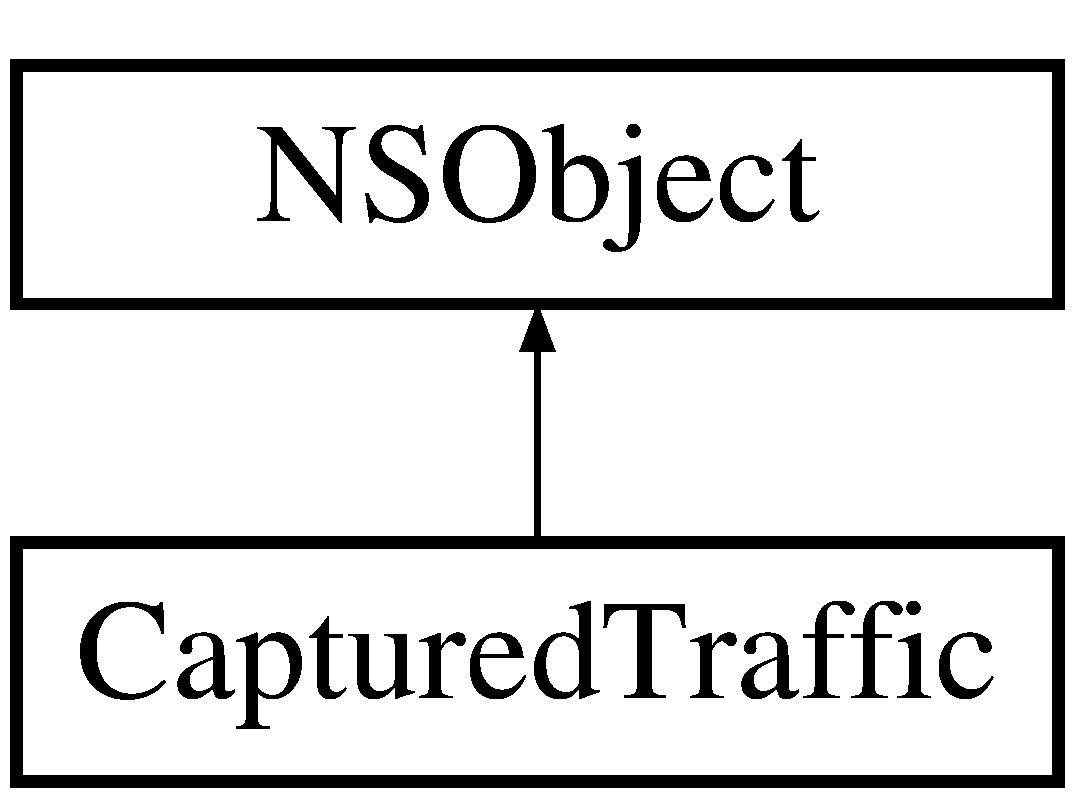
\includegraphics[height=2.000000cm]{interface_captured_traffic}
\end{center}
\end{figure}
\subsection*{Instance Methods}
\begin{DoxyCompactItemize}
\item 
\mbox{\Hypertarget{interface_captured_traffic_acdd5b72302022b9be357560878784ea9}\label{interface_captured_traffic_acdd5b72302022b9be357560878784ea9}} 
(id) -\/ {\bfseries init}
\item 
\mbox{\Hypertarget{interface_captured_traffic_a3da8260e570235ac807c02de279467f2}\label{interface_captured_traffic_a3da8260e570235ac807c02de279467f2}} 
(N\+S\+Integer) -\/ {\bfseries number\+Of\+Hosts}
\item 
\mbox{\Hypertarget{interface_captured_traffic_a1f8959e9fd8fe8815db3ed69e146ef88}\label{interface_captured_traffic_a1f8959e9fd8fe8815db3ed69e146ef88}} 
(\hyperlink{interface_traffic_for_host}{Traffic\+For\+Host} $\ast$) -\/ {\bfseries host\+At\+Index\+:}
\item 
\mbox{\Hypertarget{interface_captured_traffic_afe61d80050dddc768880b712efa5d6d1}\label{interface_captured_traffic_afe61d80050dddc768880b712efa5d6d1}} 
(N\+S\+Integer) -\/ {\bfseries index\+For\+Host\+:}
\item 
\mbox{\Hypertarget{interface_captured_traffic_aebedaa145f8a2ad119043f046d10fda1}\label{interface_captured_traffic_aebedaa145f8a2ad119043f046d10fda1}} 
(\hyperlink{interface_traffic_for_host}{Traffic\+For\+Host} $\ast$) -\/ {\bfseries for\+Host\+:}
\item 
\mbox{\Hypertarget{interface_captured_traffic_a6d2a57254bf7543f3693870027802c36}\label{interface_captured_traffic_a6d2a57254bf7543f3693870027802c36}} 
(bool) -\/ {\bfseries has\+Host\+:}
\item 
(\hyperlink{interface_traffic_for_host}{Traffic\+For\+Host} $\ast$) -\/ \hyperlink{interface_captured_traffic_a134d3585d95975a5067d01602bed36bb}{add\+Host\+:}
\item 
\mbox{\Hypertarget{interface_captured_traffic_afe6d2922f5e3b1815b3bbaaed3afdc47}\label{interface_captured_traffic_afe6d2922f5e3b1815b3bbaaed3afdc47}} 
(void) -\/ {\bfseries add\+Traffic\+For\+Host\+:transaction\+:}
\item 
\mbox{\Hypertarget{interface_captured_traffic_ad392586d3ba46d237c82bbbbc5be1f1e}\label{interface_captured_traffic_ad392586d3ba46d237c82bbbbc5be1f1e}} 
(void) -\/ {\bfseries clear}
\item 
(N\+S\+Integer) -\/ \hyperlink{interface_captured_traffic_a0acba96e0a2c8ffacfbb79fa7da8966b}{outline\+View\+:number\+Of\+Children\+Of\+Item\+:}
\begin{DoxyCompactList}\small\item\em These are data\+Source methods for N\+S\+Outline\+View. \end{DoxyCompactList}\item 
\mbox{\Hypertarget{interface_captured_traffic_a62ec426aa8a586c5c9ffabf399d964fe}\label{interface_captured_traffic_a62ec426aa8a586c5c9ffabf399d964fe}} 
(B\+O\+OL) -\/ {\bfseries outline\+View\+:is\+Item\+Expandable\+:}
\item 
\mbox{\Hypertarget{interface_captured_traffic_a0f13201fd16c07b5ebe47c7a4bb843ab}\label{interface_captured_traffic_a0f13201fd16c07b5ebe47c7a4bb843ab}} 
(id) -\/ {\bfseries outline\+View\+:child\+:of\+Item\+:}
\item 
\mbox{\Hypertarget{interface_captured_traffic_a447c2410e55e08847977062de9fcc513}\label{interface_captured_traffic_a447c2410e55e08847977062de9fcc513}} 
(id) -\/ {\bfseries outline\+View\+:object\+Value\+For\+Table\+Column\+:by\+Item\+:}
\item 
(N\+S\+View $\ast$) -\/ \hyperlink{interface_captured_traffic_a819263857354e5b56f58dbe5995aaf8c}{outline\+View\+:view\+For\+Table\+Column\+:item\+:}
\item 
\mbox{\Hypertarget{interface_captured_traffic_afb2e31d71090a37c29453ae53633c0e8}\label{interface_captured_traffic_afb2e31d71090a37c29453ae53633c0e8}} 
(N\+S\+Cell $\ast$) -\/ \hyperlink{interface_captured_traffic_afb2e31d71090a37c29453ae53633c0e8}{outline\+View\+:data\+Cell\+For\+Table\+Column\+:item\+:}
\begin{DoxyCompactList}\small\item\em returns the cell to display \end{DoxyCompactList}\item 
\mbox{\Hypertarget{interface_captured_traffic_aa8f74331f08776a7ff30a6cad7f48783}\label{interface_captured_traffic_aa8f74331f08776a7ff30a6cad7f48783}} 
(B\+O\+OL) -\/ \hyperlink{interface_captured_traffic_aa8f74331f08776a7ff30a6cad7f48783}{outline\+View\+:should\+Show\+Outline\+Cell\+For\+Item\+:}
\begin{DoxyCompactList}\small\item\em if true shows the expand triangle \end{DoxyCompactList}\item 
\mbox{\Hypertarget{interface_captured_traffic_a4615e3cad4f8a4b7443096c1180cd791}\label{interface_captured_traffic_a4615e3cad4f8a4b7443096c1180cd791}} 
(B\+O\+OL) -\/ {\bfseries outline\+View\+:should\+Expand\+Item\+:}
\item 
\mbox{\Hypertarget{interface_captured_traffic_a2a48a763f58d06e0d0f76b4fc25cbd68}\label{interface_captured_traffic_a2a48a763f58d06e0d0f76b4fc25cbd68}} 
(B\+O\+OL) -\/ {\bfseries outline\+View\+:should\+Collapse\+Item\+:}
\item 
\mbox{\Hypertarget{interface_captured_traffic_a33aecc5285a4240cfaf18f9f6fbc706e}\label{interface_captured_traffic_a33aecc5285a4240cfaf18f9f6fbc706e}} 
(B\+O\+OL) -\/ {\bfseries outline\+View\+:should\+Edit\+Table\+Column\+:item\+:}
\item 
\mbox{\Hypertarget{interface_captured_traffic_a2cf9d9ebaf56e1f0f77608b43cc3b03f}\label{interface_captured_traffic_a2cf9d9ebaf56e1f0f77608b43cc3b03f}} 
(B\+O\+OL) -\/ {\bfseries outline\+View\+:should\+Select\+Item\+:}
\item 
\mbox{\Hypertarget{interface_captured_traffic_a0ccd600588949a0b9c965e7d0fcb53ec}\label{interface_captured_traffic_a0ccd600588949a0b9c965e7d0fcb53ec}} 
(void) -\/ {\bfseries outline\+View\+Selection\+Did\+Change\+:}
\item 
\mbox{\Hypertarget{interface_captured_traffic_aa2b4f4a337e6a21450dc24664f8e6ab1}\label{interface_captured_traffic_aa2b4f4a337e6a21450dc24664f8e6ab1}} 
(void) -\/ {\bfseries outline\+View\+:will\+Display\+Outline\+Cell\+:for\+Table\+Column\+:item\+:}
\end{DoxyCompactItemize}
\subsection*{Properties}
\begin{DoxyCompactItemize}
\item 
\mbox{\Hypertarget{interface_captured_traffic_a3a7a0e2fcfbe818dff4f03fb43d8c7f9}\label{interface_captured_traffic_a3a7a0e2fcfbe818dff4f03fb43d8c7f9}} 
View\+Controller $\ast$ {\bfseries view\+Controller}
\end{DoxyCompactItemize}


\subsection{Method Documentation}
\mbox{\Hypertarget{interface_captured_traffic_a134d3585d95975a5067d01602bed36bb}\label{interface_captured_traffic_a134d3585d95975a5067d01602bed36bb}} 
\index{Captured\+Traffic@{Captured\+Traffic}!add\+Host\+:@{add\+Host\+:}}
\index{add\+Host\+:@{add\+Host\+:}!Captured\+Traffic@{Captured\+Traffic}}
\subsubsection{\texorpdfstring{add\+Host\+:()}{addHost:()}}
{\footnotesize\ttfamily -\/ (\hyperlink{interface_traffic_for_host}{Traffic\+For\+Host} $\ast$) add\+Host\+: \begin{DoxyParamCaption}\item[{(N\+S\+String$\ast$)}]{host }\end{DoxyParamCaption}}

nothing \mbox{\Hypertarget{interface_captured_traffic_a0acba96e0a2c8ffacfbb79fa7da8966b}\label{interface_captured_traffic_a0acba96e0a2c8ffacfbb79fa7da8966b}} 
\index{Captured\+Traffic@{Captured\+Traffic}!outline\+View\+:number\+Of\+Children\+Of\+Item\+:@{outline\+View\+:number\+Of\+Children\+Of\+Item\+:}}
\index{outline\+View\+:number\+Of\+Children\+Of\+Item\+:@{outline\+View\+:number\+Of\+Children\+Of\+Item\+:}!Captured\+Traffic@{Captured\+Traffic}}
\subsubsection{\texorpdfstring{outline\+View\+:number\+Of\+Children\+Of\+Item\+:()}{outlineView:numberOfChildrenOfItem:()}}
{\footnotesize\ttfamily -\/ (N\+S\+Integer) outline\+View\+: \begin{DoxyParamCaption}\item[{(N\+S\+Outline\+View $\ast$)}]{outline\+View }\item[{numberOfChildrenOfItem:(id)}]{item }\end{DoxyParamCaption}}



These are data\+Source methods for N\+S\+Outline\+View. 

N\+Outline\+View data\+Source methods 

Provided by category \hyperlink{category_captured_traffic_07_data_source_08_a0acba96e0a2c8ffacfbb79fa7da8966b}{Captured\+Traffic(\+Data\+Source)}.

\mbox{\Hypertarget{interface_captured_traffic_a819263857354e5b56f58dbe5995aaf8c}\label{interface_captured_traffic_a819263857354e5b56f58dbe5995aaf8c}} 
\index{Captured\+Traffic@{Captured\+Traffic}!outline\+View\+:view\+For\+Table\+Column\+:item\+:@{outline\+View\+:view\+For\+Table\+Column\+:item\+:}}
\index{outline\+View\+:view\+For\+Table\+Column\+:item\+:@{outline\+View\+:view\+For\+Table\+Column\+:item\+:}!Captured\+Traffic@{Captured\+Traffic}}
\subsubsection{\texorpdfstring{outline\+View\+:view\+For\+Table\+Column\+:item\+:()}{outlineView:viewForTableColumn:item:()}}
{\footnotesize\ttfamily -\/ (N\+S\+View $\ast$) outline\+View\+: \begin{DoxyParamCaption}\item[{(N\+S\+Outline\+View $\ast$)}]{outline\+View }\item[{viewForTableColumn:(N\+S\+Table\+Column $\ast$)}]{table\+Column }\item[{item:(id)}]{item }\end{DoxyParamCaption}}

N\+S\+Outline\+View delegate methods 

Provided by category \hyperlink{category_captured_traffic_07_delegate_08_a819263857354e5b56f58dbe5995aaf8c}{Captured\+Traffic(\+Delegate)}.



The documentation for this class was generated from the following files\+:\begin{DoxyCompactItemize}
\item 
marvin/objc/traffic/Captured\+Traffic.\+h\item 
marvin/objc/traffic/Captured\+Traffic.\+m\end{DoxyCompactItemize}

\hypertarget{category_captured_traffic_07_data_source_08}{}\section{Captured\+Traffic(Data\+Source) Category Reference}
\label{category_captured_traffic_07_data_source_08}\index{Captured\+Traffic(\+Data\+Source)@{Captured\+Traffic(\+Data\+Source)}}
\subsection*{Instance Methods}
\begin{DoxyCompactItemize}
\item 
(N\+S\+Integer) -\/ \hyperlink{category_captured_traffic_07_data_source_08_a0acba96e0a2c8ffacfbb79fa7da8966b}{outline\+View\+:number\+Of\+Children\+Of\+Item\+:}
\begin{DoxyCompactList}\small\item\em These are data\+Source methods for N\+S\+Outline\+View. \end{DoxyCompactList}\item 
\mbox{\Hypertarget{category_captured_traffic_07_data_source_08_a62ec426aa8a586c5c9ffabf399d964fe}\label{category_captured_traffic_07_data_source_08_a62ec426aa8a586c5c9ffabf399d964fe}} 
(B\+O\+OL) -\/ {\bfseries outline\+View\+:is\+Item\+Expandable\+:}
\item 
\mbox{\Hypertarget{category_captured_traffic_07_data_source_08_a0f13201fd16c07b5ebe47c7a4bb843ab}\label{category_captured_traffic_07_data_source_08_a0f13201fd16c07b5ebe47c7a4bb843ab}} 
(id) -\/ {\bfseries outline\+View\+:child\+:of\+Item\+:}
\item 
\mbox{\Hypertarget{category_captured_traffic_07_data_source_08_a447c2410e55e08847977062de9fcc513}\label{category_captured_traffic_07_data_source_08_a447c2410e55e08847977062de9fcc513}} 
(id) -\/ {\bfseries outline\+View\+:object\+Value\+For\+Table\+Column\+:by\+Item\+:}
\end{DoxyCompactItemize}


\subsection{Method Documentation}
\mbox{\Hypertarget{category_captured_traffic_07_data_source_08_a0acba96e0a2c8ffacfbb79fa7da8966b}\label{category_captured_traffic_07_data_source_08_a0acba96e0a2c8ffacfbb79fa7da8966b}} 
\index{Captured\+Traffic(\+Data\+Source)@{Captured\+Traffic(\+Data\+Source)}!outline\+View\+:number\+Of\+Children\+Of\+Item\+:@{outline\+View\+:number\+Of\+Children\+Of\+Item\+:}}
\index{outline\+View\+:number\+Of\+Children\+Of\+Item\+:@{outline\+View\+:number\+Of\+Children\+Of\+Item\+:}!Captured\+Traffic(\+Data\+Source)@{Captured\+Traffic(\+Data\+Source)}}
\subsubsection{\texorpdfstring{outline\+View\+:number\+Of\+Children\+Of\+Item\+:()}{outlineView:numberOfChildrenOfItem:()}}
{\footnotesize\ttfamily -\/ (N\+S\+Integer) outline\+View\+: \begin{DoxyParamCaption}\item[{(N\+S\+Outline\+View $\ast$)}]{outline\+View }\item[{numberOfChildrenOfItem:(id)}]{item }\end{DoxyParamCaption}}



These are data\+Source methods for N\+S\+Outline\+View. 

N\+Outline\+View data\+Source methods 

Extends class \hyperlink{interface_captured_traffic_a0acba96e0a2c8ffacfbb79fa7da8966b}{Captured\+Traffic}.



The documentation for this category was generated from the following files\+:\begin{DoxyCompactItemize}
\item 
marvin/objc/traffic/Captured\+Traffic-\/datasource.\+h\item 
marvin/objc/traffic/Captured\+Traffic-\/datasource.\+m\end{DoxyCompactItemize}

\hypertarget{category_captured_traffic_07_delegate_08}{}\section{Captured\+Traffic(Delegate) Category Reference}
\label{category_captured_traffic_07_delegate_08}\index{Captured\+Traffic(\+Delegate)@{Captured\+Traffic(\+Delegate)}}
\subsection*{Instance Methods}
\begin{DoxyCompactItemize}
\item 
(N\+S\+View $\ast$) -\/ \hyperlink{category_captured_traffic_07_delegate_08_a819263857354e5b56f58dbe5995aaf8c}{outline\+View\+:view\+For\+Table\+Column\+:item\+:}
\item 
\mbox{\Hypertarget{category_captured_traffic_07_delegate_08_afb2e31d71090a37c29453ae53633c0e8}\label{category_captured_traffic_07_delegate_08_afb2e31d71090a37c29453ae53633c0e8}} 
(N\+S\+Cell $\ast$) -\/ \hyperlink{category_captured_traffic_07_delegate_08_afb2e31d71090a37c29453ae53633c0e8}{outline\+View\+:data\+Cell\+For\+Table\+Column\+:item\+:}
\begin{DoxyCompactList}\small\item\em returns the cell to display \end{DoxyCompactList}\item 
\mbox{\Hypertarget{category_captured_traffic_07_delegate_08_aa8f74331f08776a7ff30a6cad7f48783}\label{category_captured_traffic_07_delegate_08_aa8f74331f08776a7ff30a6cad7f48783}} 
(B\+O\+OL) -\/ \hyperlink{category_captured_traffic_07_delegate_08_aa8f74331f08776a7ff30a6cad7f48783}{outline\+View\+:should\+Show\+Outline\+Cell\+For\+Item\+:}
\begin{DoxyCompactList}\small\item\em if true shows the expand triangle \end{DoxyCompactList}\item 
\mbox{\Hypertarget{category_captured_traffic_07_delegate_08_a4615e3cad4f8a4b7443096c1180cd791}\label{category_captured_traffic_07_delegate_08_a4615e3cad4f8a4b7443096c1180cd791}} 
(B\+O\+OL) -\/ {\bfseries outline\+View\+:should\+Expand\+Item\+:}
\item 
\mbox{\Hypertarget{category_captured_traffic_07_delegate_08_a2a48a763f58d06e0d0f76b4fc25cbd68}\label{category_captured_traffic_07_delegate_08_a2a48a763f58d06e0d0f76b4fc25cbd68}} 
(B\+O\+OL) -\/ {\bfseries outline\+View\+:should\+Collapse\+Item\+:}
\item 
\mbox{\Hypertarget{category_captured_traffic_07_delegate_08_a33aecc5285a4240cfaf18f9f6fbc706e}\label{category_captured_traffic_07_delegate_08_a33aecc5285a4240cfaf18f9f6fbc706e}} 
(B\+O\+OL) -\/ {\bfseries outline\+View\+:should\+Edit\+Table\+Column\+:item\+:}
\item 
\mbox{\Hypertarget{category_captured_traffic_07_delegate_08_a2cf9d9ebaf56e1f0f77608b43cc3b03f}\label{category_captured_traffic_07_delegate_08_a2cf9d9ebaf56e1f0f77608b43cc3b03f}} 
(B\+O\+OL) -\/ {\bfseries outline\+View\+:should\+Select\+Item\+:}
\item 
\mbox{\Hypertarget{category_captured_traffic_07_delegate_08_a0ccd600588949a0b9c965e7d0fcb53ec}\label{category_captured_traffic_07_delegate_08_a0ccd600588949a0b9c965e7d0fcb53ec}} 
(void) -\/ {\bfseries outline\+View\+Selection\+Did\+Change\+:}
\item 
\mbox{\Hypertarget{category_captured_traffic_07_delegate_08_aa2b4f4a337e6a21450dc24664f8e6ab1}\label{category_captured_traffic_07_delegate_08_aa2b4f4a337e6a21450dc24664f8e6ab1}} 
(void) -\/ {\bfseries outline\+View\+:will\+Display\+Outline\+Cell\+:for\+Table\+Column\+:item\+:}
\end{DoxyCompactItemize}


\subsection{Method Documentation}
\mbox{\Hypertarget{category_captured_traffic_07_delegate_08_a819263857354e5b56f58dbe5995aaf8c}\label{category_captured_traffic_07_delegate_08_a819263857354e5b56f58dbe5995aaf8c}} 
\index{Captured\+Traffic(\+Delegate)@{Captured\+Traffic(\+Delegate)}!outline\+View\+:view\+For\+Table\+Column\+:item\+:@{outline\+View\+:view\+For\+Table\+Column\+:item\+:}}
\index{outline\+View\+:view\+For\+Table\+Column\+:item\+:@{outline\+View\+:view\+For\+Table\+Column\+:item\+:}!Captured\+Traffic(\+Delegate)@{Captured\+Traffic(\+Delegate)}}
\subsubsection{\texorpdfstring{outline\+View\+:view\+For\+Table\+Column\+:item\+:()}{outlineView:viewForTableColumn:item:()}}
{\footnotesize\ttfamily -\/ (N\+S\+View $\ast$) outline\+View\+: \begin{DoxyParamCaption}\item[{(N\+S\+Outline\+View $\ast$)}]{outline\+View }\item[{viewForTableColumn:(N\+S\+Table\+Column $\ast$)}]{table\+Column }\item[{item:(id)}]{item }\end{DoxyParamCaption}}

N\+S\+Outline\+View delegate methods 

Extends class \hyperlink{interface_captured_traffic_a819263857354e5b56f58dbe5995aaf8c}{Captured\+Traffic}.



The documentation for this category was generated from the following files\+:\begin{DoxyCompactItemize}
\item 
marvin/objc/traffic/Captured\+Traffic-\/delegate.\+h\item 
marvin/objc/traffic/Captured\+Traffic-\/delegate.\+m\end{DoxyCompactItemize}

\hypertarget{class_marvin_1_1category}{}\section{Marvin\+:\+:category Class Reference}
\label{class_marvin_1_1category}\index{Marvin\+::category@{Marvin\+::category}}
Inheritance diagram for Marvin\+:\+:category\+:\begin{figure}[H]
\begin{center}
\leavevmode
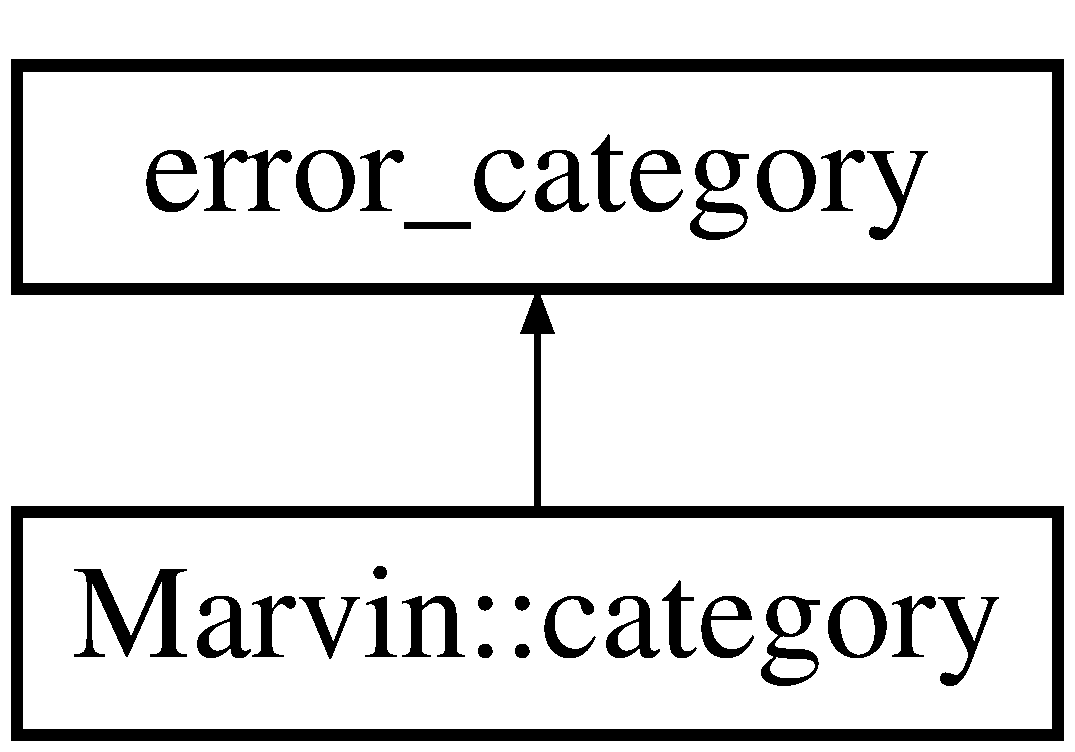
\includegraphics[height=2.000000cm]{class_marvin_1_1category}
\end{center}
\end{figure}
\subsection*{Public Member Functions}
\begin{DoxyCompactItemize}
\item 
\mbox{\Hypertarget{class_marvin_1_1category_ae34f37940b43cfc4e423549177c811e7}\label{class_marvin_1_1category_ae34f37940b43cfc4e423549177c811e7}} 
const char $\ast$ {\bfseries name} () const noexcept
\item 
\mbox{\Hypertarget{class_marvin_1_1category_a427051ac45bd66c690fd431a5e5846b7}\label{class_marvin_1_1category_a427051ac45bd66c690fd431a5e5846b7}} 
std\+::string {\bfseries message} (int ev) const
\end{DoxyCompactItemize}


The documentation for this class was generated from the following files\+:\begin{DoxyCompactItemize}
\item 
marvin/error/marvin\+\_\+error.\+hpp\item 
marvin/error/marvin\+\_\+error.\+cpp\end{DoxyCompactItemize}

\hypertarget{class_client}{}\section{Client Class Reference}
\label{class_client}\index{Client@{Client}}


{\ttfamily \#include $<$client.\+hpp$>$}

\subsection*{Public Member Functions}
\begin{DoxyCompactItemize}
\item 
\hyperlink{class_client_afdde66898aa2cbfbdace6098de0f0800}{Client} (boost\+::asio\+::io\+\_\+service \&io, Http\+Header\+::\+Scheme\+Type scheme, std\+::string server, std\+::string port)
\item 
\hyperlink{class_client_a17e2ff6c5015bea27259c47b5948c2e7}{Client} (boost\+::asio\+::io\+\_\+service \&io, std\+::string uri)
\item 
\hyperlink{class_client_a71e7eb95dbfbf747395904e04370c3b3}{Client} (boost\+::asio\+::io\+\_\+service \&io, \hyperlink{class_connection_interface}{Connection\+Interface} $\ast$conn)
\item 
\mbox{\Hypertarget{class_client_a831c9bf9b4d6907ec23a04025810693f}\label{class_client_a831c9bf9b4d6907ec23a04025810693f}} 
{\bfseries Client} (const \hyperlink{class_client}{Client} \&other)=delete
\item 
\mbox{\Hypertarget{class_client_a255f4905a3a0176a194e4a675d0a172b}\label{class_client_a255f4905a3a0176a194e4a675d0a172b}} 
\hyperlink{class_client}{Client} \& {\bfseries operator=} (const \hyperlink{class_client}{Client} \&)=delete
\item 
\mbox{\Hypertarget{class_client_a5886919756e3f0dcc4058ccb47ba44d6}\label{class_client_a5886919756e3f0dcc4058ccb47ba44d6}} 
Message\+Reader\+S\+Ptr {\bfseries get\+Response} ()
\item 
\mbox{\Hypertarget{class_client_af41106f498418bfd27f2acac18f154a5}\label{class_client_af41106f498418bfd27f2acac18f154a5}} 
void {\bfseries set\+Url} (std\+::string url)
\item 
\mbox{\Hypertarget{class_client_af1dd3726ed7b178f6adcdc97523388d3}\label{class_client_af1dd3726ed7b178f6adcdc97523388d3}} 
void {\bfseries set\+Content} (std\+::string \&content\+Str)
\item 
void \hyperlink{class_client_af87e3114d4bff798cc9f16169319b576}{set\+On\+Response} (Response\+Handler\+Callback\+Type cb)
\item 
void \hyperlink{class_client_a1d175afa24c28766e3955f7039183b6e}{set\+On\+Headers} (Response\+Handler\+Callback\+Type cb)
\item 
void \hyperlink{class_client_a73e292408e166316e14651941c92f615}{set\+On\+Data} (Client\+Data\+Handler\+Callback\+Type cb)
\item 
void \hyperlink{class_client_a7a272658b966e26a452eeaca461f8fd2}{async\+Connect} (Error\+Only\+Callback\+Type cb)
\item 
void \hyperlink{class_client_a7d9c259aa4e1262987eb3d4e909565e2}{async\+Write} (Message\+Base\+S\+Ptr request\+Message, Response\+Handler\+Callback\+Type cb)
\item 
void \hyperlink{class_client_a4cc4752e98a0466c1dcbfb6791f1e226}{async\+Write} (Message\+Base\+S\+Ptr request\+Message, std\+::string \&body\+\_\+str, Response\+Handler\+Callback\+Type cb)
\item 
\mbox{\Hypertarget{class_client_ac3481f3e23665c4a4ddabd03eec6575d}\label{class_client_ac3481f3e23665c4a4ddabd03eec6575d}} 
void {\bfseries async\+Write} (Message\+Base\+S\+Ptr request\+Message, M\+Buffer\+S\+Ptr body\+\_\+sptr, Response\+Handler\+Callback\+Type cb)
\item 
\mbox{\Hypertarget{class_client_a7048efd28cbe37f69fc9a607e2d07852}\label{class_client_a7048efd28cbe37f69fc9a607e2d07852}} 
void {\bfseries async\+Write} (Message\+Base\+S\+Ptr request\+Message, Buffer\+Chain\+S\+Ptr chain\+\_\+sptr, Response\+Handler\+Callback\+Type cb)
\item 
void \hyperlink{class_client_aecccd1b8c74dc9c0df4e211a0625391b}{async\+Write} (Message\+Base\+S\+Ptr request\+Message, F\+Buffer\+Shared\+Ptr body, Response\+Handler\+Callback\+Type cb)
\item 
void \hyperlink{class_client_a41a1654e97f9bd05ef1022076be0667c}{async\+Write\+Headers} (Message\+Base\+S\+Ptr request\+Message, Write\+Headers\+Callback\+Type cb)
\item 
void \hyperlink{class_client_a250fc2560b361f3fa3ef4a20061089d9}{async\+Write\+Body\+Data} (void $\ast$data\+Buffer, bool last, Write\+Body\+Data\+Callback\+Type cb)
\item 
void \hyperlink{class_client_ab55418abd09e5c887168d1fdf3bd9d1f}{async\+Write\+Trailers} (Message\+Base\+S\+Ptr request\+Message, Async\+Write\+Callback\+Type cb)
\item 
void \hyperlink{class_client_ae60322d424fa33d49cd88e6bee08e7af}{end} ()
\item 
void \hyperlink{class_client_a2ac4838875e743af25125d8b5c8eba09}{close} ()
\end{DoxyCompactItemize}
\subsection*{Protected Member Functions}
\begin{DoxyCompactItemize}
\item 
\mbox{\Hypertarget{class_client_a65270d4bec13972dc19c3eeab2b9c7a3}\label{class_client_a65270d4bec13972dc19c3eeab2b9c7a3}} 
void {\bfseries internal\+Connect} ()
\item 
\mbox{\Hypertarget{class_client_ab9775fe0ef908d59a5ab17e27caa8fd8}\label{class_client_ab9775fe0ef908d59a5ab17e27caa8fd8}} 
void {\bfseries internal\+Write} ()
\item 
\mbox{\Hypertarget{class_client_ab58ce4f6c733f1ecf42e4aa4007f52b2}\label{class_client_ab58ce4f6c733f1ecf42e4aa4007f52b2}} 
void {\bfseries \+\_\+async\+\_\+write} (Message\+Base\+S\+Ptr request\+Message, Response\+Handler\+Callback\+Type cb)
\item 
\mbox{\Hypertarget{class_client_a299af80ea0a0a71458a7ca4c91bc6ae7}\label{class_client_a299af80ea0a0a71458a7ca4c91bc6ae7}} 
void {\bfseries put\+Headers\+Stuff\+In\+Buffer} ()
\item 
void \hyperlink{class_client_a6d0d6b3a672370c201a24c839c5f7382}{setup\+Url} (std\+::string url)
\item 
\mbox{\Hypertarget{class_client_a2a4105d8c58e9c8e2ca1919baca31026}\label{class_client_a2a4105d8c58e9c8e2ca1919baca31026}} 
void {\bfseries default\+Headers} ()
\item 
\mbox{\Hypertarget{class_client_aedea5f9f1f9fb7a8732dc982a0e629c9}\label{class_client_aedea5f9f1f9fb7a8732dc982a0e629c9}} 
void {\bfseries set\+Content\+Length} ()
\end{DoxyCompactItemize}
\subsection*{Protected Attributes}
\begin{DoxyCompactItemize}
\item 
\mbox{\Hypertarget{class_client_a714da8195cfe69bbb8fa1f254cfa53cd}\label{class_client_a714da8195cfe69bbb8fa1f254cfa53cd}} 
std\+::string {\bfseries \+\_\+url}
\item 
\mbox{\Hypertarget{class_client_ade1bbfabad2a418db11741f9d6aef1de}\label{class_client_ade1bbfabad2a418db11741f9d6aef1de}} 
std\+::string {\bfseries \+\_\+uri}
\item 
\mbox{\Hypertarget{class_client_a9080780007752190a708d566ed3a05f0}\label{class_client_a9080780007752190a708d566ed3a05f0}} 
std\+::string {\bfseries \+\_\+scheme}
\item 
\mbox{\Hypertarget{class_client_a70d16da0e37d8395bab50d56c82d6aef}\label{class_client_a70d16da0e37d8395bab50d56c82d6aef}} 
std\+::string {\bfseries \+\_\+server}
\item 
\mbox{\Hypertarget{class_client_a9b53e47e860f4656b348654643ddb76e}\label{class_client_a9b53e47e860f4656b348654643ddb76e}} 
std\+::string {\bfseries \+\_\+host}
\item 
\mbox{\Hypertarget{class_client_a0984cf4f6e5d4a99e72b7189ab50826f}\label{class_client_a0984cf4f6e5d4a99e72b7189ab50826f}} 
std\+::string {\bfseries \+\_\+host\+\_\+with\+\_\+port}
\item 
\mbox{\Hypertarget{class_client_a4671a4ffec3179a0ba4821b0d781b901}\label{class_client_a4671a4ffec3179a0ba4821b0d781b901}} 
std\+::string {\bfseries \+\_\+port}
\item 
\mbox{\Hypertarget{class_client_a1c8113f51275dbb67633548399595ddc}\label{class_client_a1c8113f51275dbb67633548399595ddc}} 
std\+::string {\bfseries \+\_\+path}
\item 
\mbox{\Hypertarget{class_client_a4f5a6400fbe272f8212a88155cf7deb5}\label{class_client_a4f5a6400fbe272f8212a88155cf7deb5}} 
Url\+::\+Query {\bfseries \+\_\+query}
\item 
\mbox{\Hypertarget{class_client_afdcff50a83d67c071ebac089b21b16a1}\label{class_client_afdcff50a83d67c071ebac089b21b16a1}} 
std\+::string {\bfseries \+\_\+query\+Str}
\item 
\mbox{\Hypertarget{class_client_a6461a9372edd60a8aba63ae5ccc082fb}\label{class_client_a6461a9372edd60a8aba63ae5ccc082fb}} 
boost\+::asio\+::io\+\_\+service \& {\bfseries \+\_\+io}
\item 
\mbox{\Hypertarget{class_client_a4a87fac91903111214bfc059a871a5ba}\label{class_client_a4a87fac91903111214bfc059a871a5ba}} 
Message\+Base\+S\+Ptr {\bfseries \+\_\+current\+\_\+request}
\item 
\mbox{\Hypertarget{class_client_ae61b6b1b65599c17c28f8627760ea684}\label{class_client_ae61b6b1b65599c17c28f8627760ea684}} 
M\+Buffer\+S\+Ptr {\bfseries \+\_\+body\+\_\+mbuffer\+\_\+sptr}
\item 
\mbox{\Hypertarget{class_client_abc69353f4a7afea1d9a485de18350c08}\label{class_client_abc69353f4a7afea1d9a485de18350c08}} 
F\+Buffer\+Shared\+Ptr {\bfseries \+\_\+body\+\_\+fbuffer\+\_\+sptr}
\item 
\mbox{\Hypertarget{class_client_a60ba27f037924a099b13dcbace4425cc}\label{class_client_a60ba27f037924a099b13dcbace4425cc}} 
std\+::shared\+\_\+ptr$<$ \hyperlink{class_message_writer}{Message\+Writer} $>$ {\bfseries \+\_\+wrtr}
\item 
\mbox{\Hypertarget{class_client_a27fdd6a6489468f01efa06f8376bf9bb}\label{class_client_a27fdd6a6489468f01efa06f8376bf9bb}} 
std\+::shared\+\_\+ptr$<$ \hyperlink{class_message_reader}{Message\+Reader} $>$ {\bfseries \+\_\+rdr}
\item 
\mbox{\Hypertarget{class_client_a4e06284228a92f6e91b00ef170fc6ae1}\label{class_client_a4e06284228a92f6e91b00ef170fc6ae1}} 
std\+::shared\+\_\+ptr$<$ \hyperlink{class_t_c_p_connection}{T\+C\+P\+Connection} $>$ {\bfseries \+\_\+conn\+\_\+shared\+\_\+ptr}
\item 
\mbox{\Hypertarget{class_client_a3291b49a7c5c40886e31aa05a562602f}\label{class_client_a3291b49a7c5c40886e31aa05a562602f}} 
\hyperlink{class_read_socket_interface}{Read\+Socket\+Interface} $\ast$ {\bfseries \+\_\+read\+Sock}
\item 
\mbox{\Hypertarget{class_client_a02e33df170f88dbda08fe9cd0b3a0025}\label{class_client_a02e33df170f88dbda08fe9cd0b3a0025}} 
std\+::function$<$ void(Marvin\+::\+Error\+Type \&err)$>$ {\bfseries \+\_\+go\+Cb}
\item 
\mbox{\Hypertarget{class_client_a8d085507b14c836cbda0749ca2decb56}\label{class_client_a8d085507b14c836cbda0749ca2decb56}} 
Response\+Handler\+Callback\+Type {\bfseries \+\_\+response\+\_\+handler}
\item 
\mbox{\Hypertarget{class_client_ab417dd0da30a89767811a717b5c6a14f}\label{class_client_ab417dd0da30a89767811a717b5c6a14f}} 
Response\+Handler\+Callback\+Type {\bfseries \+\_\+on\+\_\+headers\+\_\+handler}
\item 
\mbox{\Hypertarget{class_client_af785f3d2d211634bf74dd35c5b523f75}\label{class_client_af785f3d2d211634bf74dd35c5b523f75}} 
Client\+Data\+Handler\+Callback\+Type {\bfseries \+\_\+on\+\_\+data\+\_\+handler}
\end{DoxyCompactItemize}
\subsection*{Friends}
\begin{DoxyCompactItemize}
\item 
\mbox{\Hypertarget{class_client_abaaeecb3bd7e6e64684e894e64752cfc}\label{class_client_abaaeecb3bd7e6e64684e894e64752cfc}} 
std\+::string {\bfseries trace\+Client} (\hyperlink{class_client}{Client} \&client)
\item 
\mbox{\Hypertarget{class_client_ad5f4b9cead705423379f0778f53e9d20}\label{class_client_ad5f4b9cead705423379f0778f53e9d20}} 
std\+::string {\bfseries trace\+Request\+Message} (\hyperlink{class_message_base}{Message\+Base} \&request)
\end{DoxyCompactItemize}


\subsection{Detailed Description}
This class implements an http client that can send a request message and wait for a response.

Two modes of transmission operation are provided for\+:


\begin{DoxyItemize}
\item send the entire request in a single call using async\+Write. This mode is best when either there is NO message body or the entire message body is available at the time the request transmission is started. In this mode the handler provided to async\+Write is passed a complete response including any body data.
\item send the request/message piecemeal -\/ headers, followed by multiple chunks of body, followed by trailers. This mode is intended to handle streaming of the body data to avoid latency or buffering large body. In this mode the handler for the incoming response message is provide by the set\+On\+Response\+Handler. The response handler should be set before any transmission is started. A complete response including body data is provided to this handler.
\end{DoxyItemize}

Two constructors are provided
\begin{DoxyItemize}
\item one will construct a non-\/connected client for which an explicit or implicit connect call will be required.
\item the other creates a client with an established connection.
\end{DoxyItemize}

Handlers or callbacks 

\subsection{Constructor \& Destructor Documentation}
\mbox{\Hypertarget{class_client_afdde66898aa2cbfbdace6098de0f0800}\label{class_client_afdde66898aa2cbfbdace6098de0f0800}} 
\index{Client@{Client}!Client@{Client}}
\index{Client@{Client}!Client@{Client}}
\subsubsection{\texorpdfstring{Client()}{Client()}\hspace{0.1cm}{\footnotesize\ttfamily [1/3]}}
{\footnotesize\ttfamily Client\+::\+Client (\begin{DoxyParamCaption}\item[{boost\+::asio\+::io\+\_\+service \&}]{io,  }\item[{Http\+Header\+::\+Scheme\+Type}]{scheme,  }\item[{std\+::string}]{server,  }\item[{std\+::string}]{port }\end{DoxyParamCaption})}

Create a client that is not connected -\/ however give it the info it needs to try and establish a connection


\begin{DoxyParams}{Parameters}
{\em io} & -\/ an io service \\
\hline
{\em scheme} & of type Http\+Header\+::\+Scheme\+Type \\
\hline
{\em server} & -\/ a string like google.\+com \\
\hline
{\em port} & -\/ a string like \char`\"{}443\char`\"{} \\
\hline
\end{DoxyParams}
\mbox{\Hypertarget{class_client_a17e2ff6c5015bea27259c47b5948c2e7}\label{class_client_a17e2ff6c5015bea27259c47b5948c2e7}} 
\index{Client@{Client}!Client@{Client}}
\index{Client@{Client}!Client@{Client}}
\subsubsection{\texorpdfstring{Client()}{Client()}\hspace{0.1cm}{\footnotesize\ttfamily [2/3]}}
{\footnotesize\ttfamily Client\+::\+Client (\begin{DoxyParamCaption}\item[{boost\+::asio\+::io\+\_\+service \&}]{io,  }\item[{std\+::string}]{uri }\end{DoxyParamCaption})}

Create a client that is not connected -\/ however give a url it needs to try and establish a connection. 
\begin{DoxyParams}{Parameters}
{\em io} & -\/ an io service \\
\hline
{\em url} & -\/ a string like \char`\"{}https\+://username\+:password@www.\+google.\+com/path1/path2\+:433?one=1111\char`\"{} \\
\hline
\end{DoxyParams}
\mbox{\Hypertarget{class_client_a71e7eb95dbfbf747395904e04370c3b3}\label{class_client_a71e7eb95dbfbf747395904e04370c3b3}} 
\index{Client@{Client}!Client@{Client}}
\index{Client@{Client}!Client@{Client}}
\subsubsection{\texorpdfstring{Client()}{Client()}\hspace{0.1cm}{\footnotesize\ttfamily [3/3]}}
{\footnotesize\ttfamily Client\+::\+Client (\begin{DoxyParamCaption}\item[{boost\+::asio\+::io\+\_\+service \&}]{io,  }\item[{\hyperlink{class_connection_interface}{Connection\+Interface} $\ast$}]{conn }\end{DoxyParamCaption})}

Create a client with an established connection. In this case a call to connect will fail with an exception -\/ as it is a logic error 

\subsection{Member Function Documentation}
\mbox{\Hypertarget{class_client_a7a272658b966e26a452eeaca461f8fd2}\label{class_client_a7a272658b966e26a452eeaca461f8fd2}} 
\index{Client@{Client}!async\+Connect@{async\+Connect}}
\index{async\+Connect@{async\+Connect}!Client@{Client}}
\subsubsection{\texorpdfstring{async\+Connect()}{asyncConnect()}}
{\footnotesize\ttfamily void Client\+::async\+Connect (\begin{DoxyParamCaption}\item[{Error\+Only\+Callback\+Type}]{cb }\end{DoxyParamCaption})}

Connects to the target host



 \subsubsection*{implement connect }\mbox{\Hypertarget{class_client_a7d9c259aa4e1262987eb3d4e909565e2}\label{class_client_a7d9c259aa4e1262987eb3d4e909565e2}} 
\index{Client@{Client}!async\+Write@{async\+Write}}
\index{async\+Write@{async\+Write}!Client@{Client}}
\subsubsection{\texorpdfstring{async\+Write()}{asyncWrite()}\hspace{0.1cm}{\footnotesize\ttfamily [1/3]}}
{\footnotesize\ttfamily void Client\+::async\+Write (\begin{DoxyParamCaption}\item[{Message\+Base\+S\+Ptr}]{request\+Message,  }\item[{Response\+Handler\+Callback\+Type}]{cb }\end{DoxyParamCaption})}

Writes the complete message to the connected host inlcuding body and trailers (if there are any).

If not connected will perform a connect before transmitting the message. Will wait for a response and call the on\+Response\+Handler CB when the response is complete.

If the request is to have a body it must be already attached to the \hyperlink{class_message_interface}{Message\+Interface}. A content\+\_\+length header will be attached by the client.

If the request is to have NO body use this method with the request\+Message.\+body == nullptr; \mbox{\Hypertarget{class_client_a4cc4752e98a0466c1dcbfb6791f1e226}\label{class_client_a4cc4752e98a0466c1dcbfb6791f1e226}} 
\index{Client@{Client}!async\+Write@{async\+Write}}
\index{async\+Write@{async\+Write}!Client@{Client}}
\subsubsection{\texorpdfstring{async\+Write()}{asyncWrite()}\hspace{0.1cm}{\footnotesize\ttfamily [2/3]}}
{\footnotesize\ttfamily void Client\+::async\+Write (\begin{DoxyParamCaption}\item[{Message\+Base\+S\+Ptr}]{request\+Message,  }\item[{std\+::string \&}]{body\+\_\+str,  }\item[{Response\+Handler\+Callback\+Type}]{cb }\end{DoxyParamCaption})}

The following are three ways to add a body to a request. The first two take a string or a shared pointer to an \hyperlink{struct_m_buffer}{M\+Buffer} -\/ these are contiguous buffers and can be sent with a single async\+Write \mbox{\Hypertarget{class_client_aecccd1b8c74dc9c0df4e211a0625391b}\label{class_client_aecccd1b8c74dc9c0df4e211a0625391b}} 
\index{Client@{Client}!async\+Write@{async\+Write}}
\index{async\+Write@{async\+Write}!Client@{Client}}
\subsubsection{\texorpdfstring{async\+Write()}{asyncWrite()}\hspace{0.1cm}{\footnotesize\ttfamily [3/3]}}
{\footnotesize\ttfamily void Client\+::async\+Write (\begin{DoxyParamCaption}\item[{Message\+Base\+S\+Ptr}]{request\+Message,  }\item[{F\+Buffer\+Shared\+Ptr}]{body,  }\item[{Response\+Handler\+Callback\+Type}]{cb }\end{DoxyParamCaption})}

The \hyperlink{class_f_buffer}{F\+Buffer} is fragmented and requires multiple async\+Write operations to send it \mbox{\Hypertarget{class_client_a250fc2560b361f3fa3ef4a20061089d9}\label{class_client_a250fc2560b361f3fa3ef4a20061089d9}} 
\index{Client@{Client}!async\+Write\+Body\+Data@{async\+Write\+Body\+Data}}
\index{async\+Write\+Body\+Data@{async\+Write\+Body\+Data}!Client@{Client}}
\subsubsection{\texorpdfstring{async\+Write\+Body\+Data()}{asyncWriteBodyData()}}
{\footnotesize\ttfamily void Client\+::async\+Write\+Body\+Data (\begin{DoxyParamCaption}\item[{void $\ast$}]{data\+Buffer,  }\item[{bool}]{last,  }\item[{Write\+Body\+Data\+Callback\+Type}]{cb }\end{DoxyParamCaption})}

Transmits a block of body data -\/ the data should N\+OT be chunk encode that will be done within the call.


\begin{DoxyParams}{Parameters}
{\em data\+Buffer} & (type T\+BD) can also be nullptr \\
\hline
{\em last} & bool -\/ signals this is the last data\+Buffer and that the chunk trailer should be generated. \\
\hline
{\em cb} & -\/ handler to be called when operation complete.\\
\hline
\end{DoxyParams}
\begin{DoxyNote}{Note}
-\/ async\+Write\+Body\+Data( nullptr, true, ....) is the normal way to
\begin{DoxyItemize}
\item signal end of data, as the caller may not know its e-\/o-\/d until after the last buffer is sent. Such a call still sends data on the connection
\begin{DoxyItemize}
\item the chunk encoding trailer. 
\end{DoxyItemize}
\end{DoxyItemize}
\end{DoxyNote}
\mbox{\Hypertarget{class_client_a41a1654e97f9bd05ef1022076be0667c}\label{class_client_a41a1654e97f9bd05ef1022076be0667c}} 
\index{Client@{Client}!async\+Write\+Headers@{async\+Write\+Headers}}
\index{async\+Write\+Headers@{async\+Write\+Headers}!Client@{Client}}
\subsubsection{\texorpdfstring{async\+Write\+Headers()}{asyncWriteHeaders()}}
{\footnotesize\ttfamily void Client\+::async\+Write\+Headers (\begin{DoxyParamCaption}\item[{Message\+Base\+S\+Ptr}]{request\+Message,  }\item[{Write\+Headers\+Callback\+Type}]{cb }\end{DoxyParamCaption})}

Sends the first line and headers of the request message only and expects any body data to be sent using async\+Write\+Body\+Data in which case the body will be \char`\"{}chunk\char`\"{} encoded and the headers will be completed to indicate this.

Dont use this method IF there is no body data, use async\+Write \mbox{\Hypertarget{class_client_ab55418abd09e5c887168d1fdf3bd9d1f}\label{class_client_ab55418abd09e5c887168d1fdf3bd9d1f}} 
\index{Client@{Client}!async\+Write\+Trailers@{async\+Write\+Trailers}}
\index{async\+Write\+Trailers@{async\+Write\+Trailers}!Client@{Client}}
\subsubsection{\texorpdfstring{async\+Write\+Trailers()}{asyncWriteTrailers()}}
{\footnotesize\ttfamily void Client\+::async\+Write\+Trailers (\begin{DoxyParamCaption}\item[{Message\+Base\+S\+Ptr}]{request\+Message,  }\item[{Async\+Write\+Callback\+Type}]{cb }\end{DoxyParamCaption})}

not yet implemented

This method should only be used if the transmission was started with a call to async\+Write\+Headers. The method async\+Write handles trailers automatically.

Sends the trailers that are present in the request\+Message -\/ trailers can be added to the message A\+F\+T\+ER transmission has started as the internals of this class do not inspect the trailers until this call nor does it keep a copy of the original request \mbox{\Hypertarget{class_client_a2ac4838875e743af25125d8b5c8eba09}\label{class_client_a2ac4838875e743af25125d8b5c8eba09}} 
\index{Client@{Client}!close@{close}}
\index{close@{close}!Client@{Client}}
\subsubsection{\texorpdfstring{close()}{close()}}
{\footnotesize\ttfamily void Client\+::close (\begin{DoxyParamCaption}{ }\end{DoxyParamCaption})}

close -\/ called to signal that connection\+::close has been received and that the net round trip should use a different connection for the next message. This invalidates \+\_\+connection, \+\_\+rdr, \+\_\+wrtr

-\/ not sure we need this -\/ just delete the client object \mbox{\Hypertarget{class_client_ae60322d424fa33d49cd88e6bee08e7af}\label{class_client_ae60322d424fa33d49cd88e6bee08e7af}} 
\index{Client@{Client}!end@{end}}
\index{end@{end}!Client@{Client}}
\subsubsection{\texorpdfstring{end()}{end()}}
{\footnotesize\ttfamily void Client\+::end (\begin{DoxyParamCaption}{ }\end{DoxyParamCaption})}

Called to signal end-\/of-\/message. This function will (if necessary) add the chunk-\/encoding trailer. \mbox{\Hypertarget{class_client_a73e292408e166316e14651941c92f615}\label{class_client_a73e292408e166316e14651941c92f615}} 
\index{Client@{Client}!set\+On\+Data@{set\+On\+Data}}
\index{set\+On\+Data@{set\+On\+Data}!Client@{Client}}
\subsubsection{\texorpdfstring{set\+On\+Data()}{setOnData()}}
{\footnotesize\ttfamily void Client\+::set\+On\+Data (\begin{DoxyParamCaption}\item[{Client\+Data\+Handler\+Callback\+Type}]{cb }\end{DoxyParamCaption})}

Sets a handler to be called when a chunk of body data is available.

optional \mbox{\Hypertarget{class_client_a1d175afa24c28766e3955f7039183b6e}\label{class_client_a1d175afa24c28766e3955f7039183b6e}} 
\index{Client@{Client}!set\+On\+Headers@{set\+On\+Headers}}
\index{set\+On\+Headers@{set\+On\+Headers}!Client@{Client}}
\subsubsection{\texorpdfstring{set\+On\+Headers()}{setOnHeaders()}}
{\footnotesize\ttfamily void Client\+::set\+On\+Headers (\begin{DoxyParamCaption}\item[{Response\+Handler\+Callback\+Type}]{cb }\end{DoxyParamCaption})}

Sets a handler to be called when all headers have been received or if an error occurs while receiving a response message headers.

optional \mbox{\Hypertarget{class_client_af87e3114d4bff798cc9f16169319b576}\label{class_client_af87e3114d4bff798cc9f16169319b576}} 
\index{Client@{Client}!set\+On\+Response@{set\+On\+Response}}
\index{set\+On\+Response@{set\+On\+Response}!Client@{Client}}
\subsubsection{\texorpdfstring{set\+On\+Response()}{setOnResponse()}}
{\footnotesize\ttfamily void Client\+::set\+On\+Response (\begin{DoxyParamCaption}\item[{Response\+Handler\+Callback\+Type}]{cb }\end{DoxyParamCaption})}

Sets a handler to be called when a complete response message is received or if an error occurs while receiving a response message. \mbox{\Hypertarget{class_client_a6d0d6b3a672370c201a24c839c5f7382}\label{class_client_a6d0d6b3a672370c201a24c839c5f7382}} 
\index{Client@{Client}!setup\+Url@{setup\+Url}}
\index{setup\+Url@{setup\+Url}!Client@{Client}}
\subsubsection{\texorpdfstring{setup\+Url()}{setupUrl()}}
{\footnotesize\ttfamily void Client\+::setup\+Url (\begin{DoxyParamCaption}\item[{std\+::string}]{url }\end{DoxyParamCaption})\hspace{0.3cm}{\ttfamily [protected]}}



 sets the url for the request, parses the url into components and saves them in particular deduces
\begin{DoxyItemize}
\item scheme
\item host -\/ both with and without port appended
\item port
\item path/uri \subsubsection*{-\/ query string }
\end{DoxyItemize}

The documentation for this class was generated from the following files\+:\begin{DoxyCompactItemize}
\item 
marvin/client/client.\+hpp\item 
marvin/client/client.\+cpp\end{DoxyCompactItemize}

\hypertarget{class_collector_base}{}\section{Collector\+Base Class Reference}
\label{class_collector_base}\index{Collector\+Base@{Collector\+Base}}
\subsection*{Public Member Functions}
\begin{DoxyCompactItemize}
\item 
\hyperlink{class_collector_base_afcc95192e8c0de4e422f615d61b28b98}{Null\+Collector} (Null\+Collector const \&)=delete
\item 
\mbox{\Hypertarget{class_collector_base_a8221d1e6914280d84fae334dfa90c011}\label{class_collector_base_a8221d1e6914280d84fae334dfa90c011}} 
void {\bfseries operator=} (\hyperlink{class_collector_base_afcc95192e8c0de4e422f615d61b28b98}{Null\+Collector} const \&)=delete
\item 
void \hyperlink{class_collector_base_a0754879d950cf3eedfaad04e9572e36c}{collect} (std\+::string \&host, Message\+Reader\+S\+Ptr req, Message\+Writer\+S\+Ptr resp)
\end{DoxyCompactItemize}
\subsection*{Static Public Member Functions}
\begin{DoxyCompactItemize}
\item 
\mbox{\Hypertarget{class_collector_base_a879b9a16e9ec5f96e69735b9ca71c9e2}\label{class_collector_base_a879b9a16e9ec5f96e69735b9ca71c9e2}} 
static \hyperlink{class_collector_base_afcc95192e8c0de4e422f615d61b28b98}{Null\+Collector} $\ast$ {\bfseries get\+Instance} (boost\+::asio\+::io\+\_\+service \&io)
\end{DoxyCompactItemize}
\subsection*{Static Public Attributes}
\begin{DoxyCompactItemize}
\item 
\mbox{\Hypertarget{class_collector_base_a7c5bda7b50244929b91a4065b88f5d6f}\label{class_collector_base_a7c5bda7b50244929b91a4065b88f5d6f}} 
static bool {\bfseries \+\_\+first\+Time}
\item 
\mbox{\Hypertarget{class_collector_base_a15463b6456436c380d18630311d1b39e}\label{class_collector_base_a15463b6456436c380d18630311d1b39e}} 
static \hyperlink{class_collector_base_afcc95192e8c0de4e422f615d61b28b98}{Null\+Collector} $\ast$ {\bfseries \+\_\+instance}
\end{DoxyCompactItemize}


\subsection{Member Function Documentation}
\mbox{\Hypertarget{class_collector_base_a0754879d950cf3eedfaad04e9572e36c}\label{class_collector_base_a0754879d950cf3eedfaad04e9572e36c}} 
\index{Collector\+Base@{Collector\+Base}!collect@{collect}}
\index{collect@{collect}!Collector\+Base@{Collector\+Base}}
\subsubsection{\texorpdfstring{collect()}{collect()}}
{\footnotesize\ttfamily void Collector\+Base\+::collect (\begin{DoxyParamCaption}\item[{std\+::string \&}]{host,  }\item[{Message\+Reader\+S\+Ptr}]{req,  }\item[{Message\+Writer\+S\+Ptr}]{resp }\end{DoxyParamCaption})}

Interface method for client code to call collect In here implement the creation the summary records but dont do any IO or sending leave that for posted\+Collect\mbox{\Hypertarget{class_collector_base_afcc95192e8c0de4e422f615d61b28b98}\label{class_collector_base_afcc95192e8c0de4e422f615d61b28b98}} 
\index{Collector\+Base@{Collector\+Base}!Null\+Collector@{Null\+Collector}}
\index{Null\+Collector@{Null\+Collector}!Collector\+Base@{Collector\+Base}}
\subsubsection{\texorpdfstring{Null\+Collector()}{NullCollector()}}
{\footnotesize\ttfamily Collector\+Base\+::\+Null\+Collector (\begin{DoxyParamCaption}\item[{Null\+Collector const \&}]{ }\end{DoxyParamCaption})\hspace{0.3cm}{\ttfamily [delete]}}

Delete copy constructors 

The documentation for this class was generated from the following files\+:\begin{DoxyCompactItemize}
\item 
marvin/collector/collector\+\_\+base.\+hpp\item 
marvin/collector/collector\+\_\+base.\+cpp\end{DoxyCompactItemize}

\hypertarget{class_connection_handler}{}\section{Connection\+Handler Class Reference}
\label{class_connection_handler}\index{Connection\+Handler@{Connection\+Handler}}
\subsection*{Public Member Functions}
\begin{DoxyCompactItemize}
\item 
\hyperlink{class_connection_handler_ad47277a5528017ca18c74c42184f506c}{Connection\+Handler} (boost\+::asio\+::io\+\_\+service \&io, \hyperlink{class_server_connection_manager}{Server\+Connection\+Manager} \&connection\+Manager, \hyperlink{class_connection_interface}{Connection\+Interface} $\ast$conn, Request\+Handler\+Factory factory)
\item 
void \hyperlink{class_connection_handler_a113fc7138a4dd5ab03fdca63091002a6}{serve} ()
\item 
long \hyperlink{class_connection_handler_a26a9c6287af17142e2497b26afd020df}{native\+Socket\+FD} ()
\item 
\mbox{\Hypertarget{class_connection_handler_a0df2d9e8522cbb736bfa3113beb6a34d}\label{class_connection_handler_a0df2d9e8522cbb736bfa3113beb6a34d}} 
std\+::string {\bfseries uuid} ()
\end{DoxyCompactItemize}


\subsection{Constructor \& Destructor Documentation}
\mbox{\Hypertarget{class_connection_handler_ad47277a5528017ca18c74c42184f506c}\label{class_connection_handler_ad47277a5528017ca18c74c42184f506c}} 
\index{Connection\+Handler@{Connection\+Handler}!Connection\+Handler@{Connection\+Handler}}
\index{Connection\+Handler@{Connection\+Handler}!Connection\+Handler@{Connection\+Handler}}
\subsubsection{\texorpdfstring{Connection\+Handler()}{ConnectionHandler()}}
{\footnotesize\ttfamily Connection\+Handler\+::\+Connection\+Handler (\begin{DoxyParamCaption}\item[{boost\+::asio\+::io\+\_\+service \&}]{io,  }\item[{\hyperlink{class_server_connection_manager}{Server\+Connection\+Manager} \&}]{connection\+Manager,  }\item[{\hyperlink{class_connection_interface}{Connection\+Interface} $\ast$}]{conn,  }\item[{Request\+Handler\+Factory}]{factory }\end{DoxyParamCaption})}

The connection and the request handler persist acrosss all messages served by a connection handler. This is required to ensure that our M\+I\+TM proxy can handle keep-\/alive

\subsection{Member Function Documentation}
\mbox{\Hypertarget{class_connection_handler_a26a9c6287af17142e2497b26afd020df}\label{class_connection_handler_a26a9c6287af17142e2497b26afd020df}} 
\index{Connection\+Handler@{Connection\+Handler}!native\+Socket\+FD@{native\+Socket\+FD}}
\index{native\+Socket\+FD@{native\+Socket\+FD}!Connection\+Handler@{Connection\+Handler}}
\subsubsection{\texorpdfstring{native\+Socket\+F\+D()}{nativeSocketFD()}}
{\footnotesize\ttfamily long Connection\+Handler\+::native\+Socket\+FD (\begin{DoxyParamCaption}{ }\end{DoxyParamCaption})}

Utility method returns the underlying FD for this connection. Used only for debug racing purposes \mbox{\Hypertarget{class_connection_handler_a113fc7138a4dd5ab03fdca63091002a6}\label{class_connection_handler_a113fc7138a4dd5ab03fdca63091002a6}} 
\index{Connection\+Handler@{Connection\+Handler}!serve@{serve}}
\index{serve@{serve}!Connection\+Handler@{Connection\+Handler}}
\subsubsection{\texorpdfstring{serve()}{serve()}}
{\footnotesize\ttfamily void Connection\+Handler\+::serve (\begin{DoxyParamCaption}{ }\end{DoxyParamCaption})}

Come here to start the read of a request message, ahdnhence start a request/response cycle 

The documentation for this class was generated from the following files\+:\begin{DoxyCompactItemize}
\item 
marvin/server/connection\+\_\+handler.\+hpp\item 
marvin/server/connection\+\_\+handler.\+cpp\end{DoxyCompactItemize}

\hypertarget{class_connection_handler_manager}{}\section{Connection\+Handler\+Manager Class Reference}
\label{class_connection_handler_manager}\index{Connection\+Handler\+Manager@{Connection\+Handler\+Manager}}
\subsection*{Public Member Functions}
\begin{DoxyCompactItemize}
\item 
\mbox{\Hypertarget{class_connection_handler_manager_a3c6a65fe45c3574fbb816224233032ae}\label{class_connection_handler_manager_a3c6a65fe45c3574fbb816224233032ae}} 
{\bfseries Connection\+Handler\+Manager} (boost\+::asio\+::io\+\_\+service \&io, boost\+::asio\+::strand \&strand)
\item 
\mbox{\Hypertarget{class_connection_handler_manager_a41e753bd06b7248fe6f4adebbe2eec05}\label{class_connection_handler_manager_a41e753bd06b7248fe6f4adebbe2eec05}} 
void {\bfseries init} (boost\+::asio\+::io\+\_\+service \&io)
\item 
\mbox{\Hypertarget{class_connection_handler_manager_a690c04e4c29cf92649148e4e03b6473e}\label{class_connection_handler_manager_a690c04e4c29cf92649148e4e03b6473e}} 
void {\bfseries async\+Acquire\+Connection\+Handler} (std\+::string scheme, std\+::string server, std\+::string port, Connect\+Callback\+Type cb)
\item 
\mbox{\Hypertarget{class_connection_handler_manager_a5931179ee0b6c4955977aa52d36f4407}\label{class_connection_handler_manager_a5931179ee0b6c4955977aa52d36f4407}} 
void {\bfseries release\+Connection\+Handler} (\hyperlink{class_connection_handler}{Connection\+Handler} $\ast$conn\+\_\+handler)
\end{DoxyCompactItemize}
\subsection*{Static Public Member Functions}
\begin{DoxyCompactItemize}
\item 
\mbox{\Hypertarget{class_connection_handler_manager_aaf3d518a261232e67ea9ff2460f67582}\label{class_connection_handler_manager_aaf3d518a261232e67ea9ff2460f67582}} 
static \hyperlink{class_connection_handler_manager}{Connection\+Handler\+Manager} $\ast$ {\bfseries get\+Instance} (boost\+::asio\+::io\+\_\+service \&io)
\end{DoxyCompactItemize}


The documentation for this class was generated from the following files\+:\begin{DoxyCompactItemize}
\item 
marvin/server/connection\+\_\+handler\+\_\+pool.\+hpp\item 
marvin/server/connection\+\_\+handler\+\_\+pool .\+cpp\end{DoxyCompactItemize}

\hypertarget{class_connection_interface}{}\section{Connection\+Interface Class Reference}
\label{class_connection_interface}\index{Connection\+Interface@{Connection\+Interface}}
Inheritance diagram for Connection\+Interface\+:\begin{figure}[H]
\begin{center}
\leavevmode
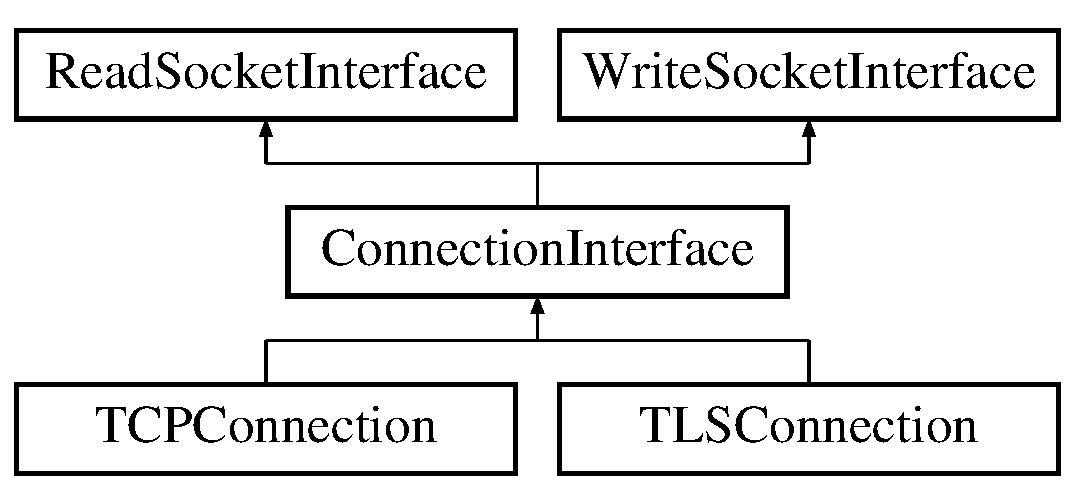
\includegraphics[height=3.000000cm]{class_connection_interface}
\end{center}
\end{figure}
\subsection*{Public Member Functions}
\begin{DoxyCompactItemize}
\item 
\mbox{\Hypertarget{class_connection_interface_a6741f1ae1b638b9bc651aafb8e0f2d3e}\label{class_connection_interface_a6741f1ae1b638b9bc651aafb8e0f2d3e}} 
virtual void {\bfseries async\+Connect} (Connect\+Callback\+Type cb)=0
\item 
\mbox{\Hypertarget{class_connection_interface_a646b195a8ca848fcc97186b48453964e}\label{class_connection_interface_a646b195a8ca848fcc97186b48453964e}} 
virtual void {\bfseries async\+Accept} (boost\+::asio\+::ip\+::tcp\+::acceptor \&acceptor, std\+::function$<$ void(const boost\+::system\+::error\+\_\+code \&err)$>$ cb)=0
\item 
\mbox{\Hypertarget{class_connection_interface_a256d0020c9bddb14c5832ff1c6278ad2}\label{class_connection_interface_a256d0020c9bddb14c5832ff1c6278ad2}} 
virtual void {\bfseries async\+Write} (\hyperlink{struct_m_buffer}{M\+Buffer} \&buffer, Async\+Write\+Callback\+Type cb)=0
\item 
\mbox{\Hypertarget{class_connection_interface_a21ea35f069518ee6489a67c27ecad1f0}\label{class_connection_interface_a21ea35f069518ee6489a67c27ecad1f0}} 
virtual void {\bfseries async\+Write} (Buffer\+Chain\+S\+Ptr buf\+\_\+chain\+\_\+sptr, Async\+Write\+Callback\+Type cb)=0
\item 
\mbox{\Hypertarget{class_connection_interface_aa8523c8458edaacc38f3e55f657f8298}\label{class_connection_interface_aa8523c8458edaacc38f3e55f657f8298}} 
virtual void {\bfseries async\+Write} (std\+::string \&str, Async\+Write\+Callback\+Type cb)=0
\item 
\mbox{\Hypertarget{class_connection_interface_a6bcdb433cfa5d6c4040d15dd64e6014b}\label{class_connection_interface_a6bcdb433cfa5d6c4040d15dd64e6014b}} 
virtual void {\bfseries async\+Write} (boost\+::asio\+::const\+\_\+buffer buf, Async\+Write\+Callback cb)=0
\item 
\mbox{\Hypertarget{class_connection_interface_a505ca3b8a542e8014b76e0a3131372ec}\label{class_connection_interface_a505ca3b8a542e8014b76e0a3131372ec}} 
virtual void {\bfseries async\+Write} (boost\+::asio\+::streambuf \&sb, Async\+Write\+Callback)=0
\item 
\mbox{\Hypertarget{class_connection_interface_a0a36ca4e4133eabbef1daeccb1f28f6c}\label{class_connection_interface_a0a36ca4e4133eabbef1daeccb1f28f6c}} 
virtual void {\bfseries shutdown} ()=0
\item 
\mbox{\Hypertarget{class_connection_interface_ab911b5babbc2321520114b302fce8df6}\label{class_connection_interface_ab911b5babbc2321520114b302fce8df6}} 
virtual void {\bfseries close} ()=0
\item 
\mbox{\Hypertarget{class_connection_interface_a5ecc247e28761248e4c5266dd871c7b6}\label{class_connection_interface_a5ecc247e28761248e4c5266dd871c7b6}} 
virtual long {\bfseries native\+Socket\+FD} ()=0
\end{DoxyCompactItemize}


The documentation for this class was generated from the following file\+:\begin{DoxyCompactItemize}
\item 
marvin/include/connection\+\_\+interface.\+hpp\end{DoxyCompactItemize}

\hypertarget{class_connection_pool}{}\section{Connection\+Pool Class Reference}
\label{class_connection_pool}\index{Connection\+Pool@{Connection\+Pool}}
\subsection*{Public Member Functions}
\begin{DoxyCompactItemize}
\item 
\mbox{\Hypertarget{class_connection_pool_a810f0b989677a5c6ec44b5d8d4f9c93f}\label{class_connection_pool_a810f0b989677a5c6ec44b5d8d4f9c93f}} 
{\bfseries Connection\+Pool} (boost\+::asio\+::io\+\_\+service \&io)
\item 
\mbox{\Hypertarget{class_connection_pool_ab8c78cedcb60144339a9e7c7426592c2}\label{class_connection_pool_ab8c78cedcb60144339a9e7c7426592c2}} 
void {\bfseries init} (boost\+::asio\+::io\+\_\+service \&io)
\item 
void \hyperlink{class_connection_pool_acc0c130e9601ab5535693a4f5618eaa1}{async\+Get\+Connection} (std\+::string scheme, std\+::string server, std\+::string port, Connect\+Callback\+Type cb)
\item 
\mbox{\Hypertarget{class_connection_pool_a5e0cc0906e72ab4e8fe553949dbe0227}\label{class_connection_pool_a5e0cc0906e72ab4e8fe553949dbe0227}} 
void {\bfseries release\+Connection} (\hyperlink{class_connection_interface}{Connection\+Interface} $\ast$conn)
\end{DoxyCompactItemize}
\subsection*{Static Public Member Functions}
\begin{DoxyCompactItemize}
\item 
\mbox{\Hypertarget{class_connection_pool_a0532d3be3aa1b46efe9d5dc4dd9d8661}\label{class_connection_pool_a0532d3be3aa1b46efe9d5dc4dd9d8661}} 
static \hyperlink{class_connection_pool}{Connection\+Pool} $\ast$ {\bfseries get\+Instance} (boost\+::asio\+::io\+\_\+service \&io)
\end{DoxyCompactItemize}


\subsection{Member Function Documentation}
\mbox{\Hypertarget{class_connection_pool_acc0c130e9601ab5535693a4f5618eaa1}\label{class_connection_pool_acc0c130e9601ab5535693a4f5618eaa1}} 
\index{Connection\+Pool@{Connection\+Pool}!async\+Get\+Connection@{async\+Get\+Connection}}
\index{async\+Get\+Connection@{async\+Get\+Connection}!Connection\+Pool@{Connection\+Pool}}
\subsubsection{\texorpdfstring{async\+Get\+Connection()}{asyncGetConnection()}}
{\footnotesize\ttfamily void Connection\+Pool\+::async\+Get\+Connection (\begin{DoxyParamCaption}\item[{std\+::string}]{scheme,  }\item[{std\+::string}]{server,  }\item[{std\+::string}]{service,  }\item[{Connect\+Callback\+Type}]{cb }\end{DoxyParamCaption})}

get a connection to the scheme\+::server 

The documentation for this class was generated from the following files\+:\begin{DoxyCompactItemize}
\item 
marvin/connection/connection\+\_\+pool.\+hpp\item 
marvin/connection/connection\+\_\+pool.\+cpp\item 
marvin/src/connection\+\_\+pool copy.\+cpp\end{DoxyCompactItemize}

\hypertarget{class_connection_request}{}\section{Connection\+Request Class Reference}
\label{class_connection_request}\index{Connection\+Request@{Connection\+Request}}
\subsection*{Public Member Functions}
\begin{DoxyCompactItemize}
\item 
\mbox{\Hypertarget{class_connection_request_a8fcda439275940ab6ce76fa11513f936}\label{class_connection_request_a8fcda439275940ab6ce76fa11513f936}} 
{\bfseries Connection\+Request} (std\+::string scheme, std\+::string server, std\+::string service, Connect\+Callback\+Type cb)
\item 
\mbox{\Hypertarget{class_connection_request_a8fcda439275940ab6ce76fa11513f936}\label{class_connection_request_a8fcda439275940ab6ce76fa11513f936}} 
{\bfseries Connection\+Request} (std\+::string scheme, std\+::string server, std\+::string service, Connect\+Callback\+Type cb)
\item 
\mbox{\Hypertarget{class_connection_request_a5db5ffeaf535b588d3d78b416395cc75}\label{class_connection_request_a5db5ffeaf535b588d3d78b416395cc75}} 
{\bfseries Connection\+Request} (std\+::string host\+Id, Connection\+Request\+Callback\+Type cb)
\end{DoxyCompactItemize}
\subsection*{Public Attributes}
\begin{DoxyCompactItemize}
\item 
\mbox{\Hypertarget{class_connection_request_ad3fb8a25086c021d65c0fa66c2e5b83c}\label{class_connection_request_ad3fb8a25086c021d65c0fa66c2e5b83c}} 
std\+::string {\bfseries \+\_\+scheme}
\item 
\mbox{\Hypertarget{class_connection_request_a76fd8c69232cb1355f14afc88ab7451e}\label{class_connection_request_a76fd8c69232cb1355f14afc88ab7451e}} 
std\+::string {\bfseries \+\_\+server}
\item 
\mbox{\Hypertarget{class_connection_request_a25c410eaa9b1890bce9bbffb2b33fc6d}\label{class_connection_request_a25c410eaa9b1890bce9bbffb2b33fc6d}} 
std\+::string {\bfseries \+\_\+service}
\item 
\mbox{\Hypertarget{class_connection_request_a849789e01011a6ac57a2adc4363a0071}\label{class_connection_request_a849789e01011a6ac57a2adc4363a0071}} 
Connect\+Callback\+Type {\bfseries \+\_\+callback}
\end{DoxyCompactItemize}


The documentation for this class was generated from the following files\+:\begin{DoxyCompactItemize}
\item 
marvin/connection/connection\+\_\+pool.\+hpp\item 
marvin/server/connection\+\_\+handler\+\_\+pool.\+hpp\item 
marvin/src/connection\+\_\+pool copy.\+cpp\item 
marvin/connection/connection\+\_\+pool.\+cpp\end{DoxyCompactItemize}

\hypertarget{class_f_buffer}{}\section{F\+Buffer Class Reference}
\label{class_f_buffer}\index{F\+Buffer@{F\+Buffer}}
\subsection*{Public Member Functions}
\begin{DoxyCompactItemize}
\item 
\hyperlink{class_f_buffer_a3aac6ae74811d7c6d3902ad5c1fdcab3}{F\+Buffer} (\hyperlink{struct_m_buffer}{M\+Buffer} $\ast$mbuf)
\item 
\hyperlink{class_f_buffer_a89680be41fb35ea1b9591ca646713f2f}{F\+Buffer} (std\+::size\+\_\+t capacity)
\item 
\hyperlink{class_f_buffer_a4e490d569edada34d24a5b16da72fafc}{$\sim$\+F\+Buffer} ()
\item 
std\+::size\+\_\+t \hyperlink{class_f_buffer_ae5f30d510287df8185bc30ecfd80840e}{size} ()
\item 
\hyperlink{struct_m_buffer}{M\+Buffer} \& \hyperlink{class_f_buffer_a0987483eef377d599dcae38a6aac5236}{get\+M\+Buffer} ()
\item 
void \hyperlink{class_f_buffer_a64064a784e0ada0957d76db6c83b22fa}{copy\+In} (void $\ast$bytes, std\+::size\+\_\+t len)
\item 
void \hyperlink{class_f_buffer_aee2d12df78293e2b3e8da359e7d0a757}{add\+Fragment} (void $\ast$bytes, std\+::size\+\_\+t len)
\end{DoxyCompactItemize}
\subsection*{Protected Attributes}
\begin{DoxyCompactItemize}
\item 
\mbox{\Hypertarget{class_f_buffer_ac9dc209989dbda81840a3cfb96de77d5}\label{class_f_buffer_ac9dc209989dbda81840a3cfb96de77d5}} 
\hyperlink{struct_m_buffer}{M\+Buffer} $\ast$ {\bfseries \+\_\+container}
\item 
\mbox{\Hypertarget{class_f_buffer_af444abbf2078dfd307692e9102a066ab}\label{class_f_buffer_af444abbf2078dfd307692e9102a066ab}} 
std\+::vector$<$ \hyperlink{class_fragment}{Fragment} $>$ \hyperlink{class_f_buffer_af444abbf2078dfd307692e9102a066ab}{\+\_\+fragments}
\begin{DoxyCompactList}\small\item\em where all the fragments reside \end{DoxyCompactList}\item 
\mbox{\Hypertarget{class_f_buffer_a5cf37f4378a3f5d778f65786a9fed276}\label{class_f_buffer_a5cf37f4378a3f5d778f65786a9fed276}} 
std\+::size\+\_\+t \hyperlink{class_f_buffer_a5cf37f4378a3f5d778f65786a9fed276}{\+\_\+size}
\begin{DoxyCompactList}\small\item\em a list of fragments \end{DoxyCompactList}\end{DoxyCompactItemize}
\subsection*{Friends}
\begin{DoxyCompactItemize}
\item 
\mbox{\Hypertarget{class_f_buffer_a2a832c78617be463503bceec23b2e773}\label{class_f_buffer_a2a832c78617be463503bceec23b2e773}} 
std\+::vector$<$ boost\+::asio\+::const\+\_\+buffer $>$ {\bfseries fb\+\_\+as\+\_\+const\+\_\+buffer\+\_\+sequence} (\hyperlink{class_f_buffer}{F\+Buffer} \&bm)
\item 
\mbox{\Hypertarget{class_f_buffer_a3e2bb2caacfd3d4795212913c14c277b}\label{class_f_buffer_a3e2bb2caacfd3d4795212913c14c277b}} 
std\+::vector$<$ boost\+::asio\+::mutable\+\_\+buffer $>$ {\bfseries fb\+\_\+as\+\_\+mutable\+\_\+buffer\+\_\+sequence} (\hyperlink{class_f_buffer}{F\+Buffer} \&bm)
\item 
\mbox{\Hypertarget{class_f_buffer_a96fce1073312fb0ff79ae8b2ae78451e}\label{class_f_buffer_a96fce1073312fb0ff79ae8b2ae78451e}} 
std\+::ostream \& {\bfseries operator$<$$<$} (std\+::ostream \&os, \hyperlink{class_f_buffer}{F\+Buffer} const \&b)
\end{DoxyCompactItemize}


\subsection{Constructor \& Destructor Documentation}
\mbox{\Hypertarget{class_f_buffer_a3aac6ae74811d7c6d3902ad5c1fdcab3}\label{class_f_buffer_a3aac6ae74811d7c6d3902ad5c1fdcab3}} 
\index{F\+Buffer@{F\+Buffer}!F\+Buffer@{F\+Buffer}}
\index{F\+Buffer@{F\+Buffer}!F\+Buffer@{F\+Buffer}}
\subsubsection{\texorpdfstring{F\+Buffer()}{FBuffer()}\hspace{0.1cm}{\footnotesize\ttfamily [1/2]}}
{\footnotesize\ttfamily F\+Buffer\+::\+F\+Buffer (\begin{DoxyParamCaption}\item[{\hyperlink{struct_m_buffer}{M\+Buffer} $\ast$}]{mbuf }\end{DoxyParamCaption})}

Constructor that wraps an \hyperlink{struct_m_buffer}{M\+Buffer} -\/ the \hyperlink{class_f_buffer}{F\+Buffer} now \char`\"{}owns\char`\"{} the \hyperlink{struct_m_buffer}{M\+Buffer} and will free/delete it in the \hyperlink{class_f_buffer}{F\+Buffer}\textquotesingle{}s destructor \mbox{\Hypertarget{class_f_buffer_a89680be41fb35ea1b9591ca646713f2f}\label{class_f_buffer_a89680be41fb35ea1b9591ca646713f2f}} 
\index{F\+Buffer@{F\+Buffer}!F\+Buffer@{F\+Buffer}}
\index{F\+Buffer@{F\+Buffer}!F\+Buffer@{F\+Buffer}}
\subsubsection{\texorpdfstring{F\+Buffer()}{FBuffer()}\hspace{0.1cm}{\footnotesize\ttfamily [2/2]}}
{\footnotesize\ttfamily F\+Buffer\+::\+F\+Buffer (\begin{DoxyParamCaption}\item[{std\+::size\+\_\+t}]{capacity }\end{DoxyParamCaption})}

Constructore that hides the underlying \hyperlink{struct_m_buffer}{M\+Buffer} \mbox{\Hypertarget{class_f_buffer_a4e490d569edada34d24a5b16da72fafc}\label{class_f_buffer_a4e490d569edada34d24a5b16da72fafc}} 
\index{F\+Buffer@{F\+Buffer}!````~F\+Buffer@{$\sim$\+F\+Buffer}}
\index{````~F\+Buffer@{$\sim$\+F\+Buffer}!F\+Buffer@{F\+Buffer}}
\subsubsection{\texorpdfstring{$\sim$\+F\+Buffer()}{~FBuffer()}}
{\footnotesize\ttfamily F\+Buffer\+::$\sim$\+F\+Buffer (\begin{DoxyParamCaption}{ }\end{DoxyParamCaption})}

Destructor -\/ will delete the managed \hyperlink{struct_m_buffer}{M\+Buffer} 

\subsection{Member Function Documentation}
\mbox{\Hypertarget{class_f_buffer_aee2d12df78293e2b3e8da359e7d0a757}\label{class_f_buffer_aee2d12df78293e2b3e8da359e7d0a757}} 
\index{F\+Buffer@{F\+Buffer}!add\+Fragment@{add\+Fragment}}
\index{add\+Fragment@{add\+Fragment}!F\+Buffer@{F\+Buffer}}
\subsubsection{\texorpdfstring{add\+Fragment()}{addFragment()}}
{\footnotesize\ttfamily void F\+Buffer\+::add\+Fragment (\begin{DoxyParamCaption}\item[{void $\ast$}]{bytes,  }\item[{std\+::size\+\_\+t}]{len }\end{DoxyParamCaption})}

add a new fragment to the \hyperlink{class_f_buffer}{F\+Buffer} check the fragment is inside address bounds of the managed \hyperlink{struct_m_buffer}{M\+Buffer} and that the new fragment is \char`\"{}past\char`\"{} (has a higher starting address) than the previously \char`\"{}last\char`\"{} fragment if this new fragment is contiguous with the \char`\"{}last\char`\"{} fragment consolidate the two if this new fragment is empty (len = 0) then do nothing \mbox{\Hypertarget{class_f_buffer_a64064a784e0ada0957d76db6c83b22fa}\label{class_f_buffer_a64064a784e0ada0957d76db6c83b22fa}} 
\index{F\+Buffer@{F\+Buffer}!copy\+In@{copy\+In}}
\index{copy\+In@{copy\+In}!F\+Buffer@{F\+Buffer}}
\subsubsection{\texorpdfstring{copy\+In()}{copyIn()}}
{\footnotesize\ttfamily void F\+Buffer\+::copy\+In (\begin{DoxyParamCaption}\item[{void $\ast$}]{bytes,  }\item[{std\+::size\+\_\+t}]{len }\end{DoxyParamCaption})}

copies these bytes into the \hyperlink{class_f_buffer}{F\+Buffer} so that they are continguous with (that is added to) the last fragement (fragment with the highest starting address) \mbox{\Hypertarget{class_f_buffer_a0987483eef377d599dcae38a6aac5236}\label{class_f_buffer_a0987483eef377d599dcae38a6aac5236}} 
\index{F\+Buffer@{F\+Buffer}!get\+M\+Buffer@{get\+M\+Buffer}}
\index{get\+M\+Buffer@{get\+M\+Buffer}!F\+Buffer@{F\+Buffer}}
\subsubsection{\texorpdfstring{get\+M\+Buffer()}{getMBuffer()}}
{\footnotesize\ttfamily \hyperlink{struct_m_buffer}{M\+Buffer}\& F\+Buffer\+::get\+M\+Buffer (\begin{DoxyParamCaption}{ }\end{DoxyParamCaption})}

Return the underlying \hyperlink{struct_m_buffer}{M\+Buffer} \mbox{\Hypertarget{class_f_buffer_ae5f30d510287df8185bc30ecfd80840e}\label{class_f_buffer_ae5f30d510287df8185bc30ecfd80840e}} 
\index{F\+Buffer@{F\+Buffer}!size@{size}}
\index{size@{size}!F\+Buffer@{F\+Buffer}}
\subsubsection{\texorpdfstring{size()}{size()}}
{\footnotesize\ttfamily std\+::size\+\_\+t F\+Buffer\+::size (\begin{DoxyParamCaption}{ }\end{DoxyParamCaption})}

Returns the total size of all fragments 

The documentation for this class was generated from the following files\+:\begin{DoxyCompactItemize}
\item 
marvin/buffer/buffer.\+hpp\item 
marvin/buffer/buffer.\+cpp\end{DoxyCompactItemize}

\hypertarget{class_forwarding_handler}{}\section{Forwarding\+Handler$<$ T\+Collector $>$ Class Template Reference}
\label{class_forwarding_handler}\index{Forwarding\+Handler$<$ T\+Collector $>$@{Forwarding\+Handler$<$ T\+Collector $>$}}


This class implements the proxy forwarding process for http/https protocols. Its a revised version to make way for future requirements of \char`\"{}replaying\char`\"{} an exchange The V2 version of this class makes the composition of functions during the forwarding process more evident.  Reads a message from the downstream client, converts that to a non-\/proxy request to the targets server, sends that request, collects the response and finally sends that response to the originating client. Along the way it captures (via template parameter T\+Capture) a summary of the original request and upstream server response and distributes that according to the rules of the particular T\+Capture object.  




{\ttfamily \#include $<$forwarding\+\_\+handler.\+hpp$>$}

Inheritance diagram for Forwarding\+Handler$<$ T\+Collector $>$\+:\begin{figure}[H]
\begin{center}
\leavevmode
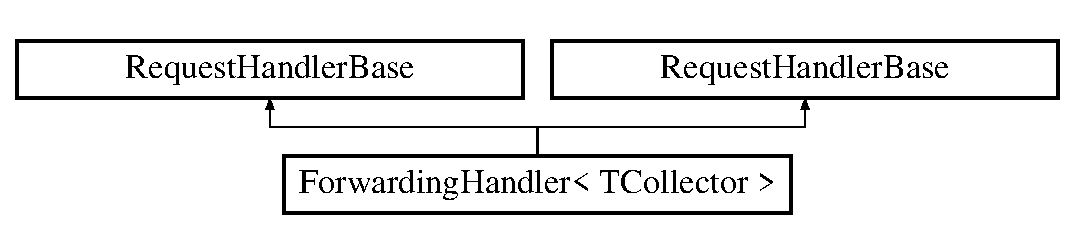
\includegraphics[height=2.000000cm]{class_forwarding_handler}
\end{center}
\end{figure}
\subsection*{Public Member Functions}
\begin{DoxyCompactItemize}
\item 
\mbox{\Hypertarget{class_forwarding_handler_a86bb59fe85fa0bc42b26715b59e34583}\label{class_forwarding_handler_a86bb59fe85fa0bc42b26715b59e34583}} 
{\bfseries Forwarding\+Handler} (boost\+::asio\+::io\+\_\+service \&io)
\item 
void \hyperlink{class_forwarding_handler_ac4f8ecec2ca1267b8fdf806c5d4cc155}{handle\+Connect} (Message\+Reader\+S\+Ptr req, Connection\+Interface\+S\+Ptr conn\+Ptr, Handler\+Done\+Callback\+Type done)
\item 
void \hyperlink{class_forwarding_handler_ab5007f621c7f0fe5a9c92b71ff6c15ef}{handle\+Request} (Message\+Reader\+S\+Ptr req, Message\+Writer\+S\+Ptr rep, Handler\+Done\+Callback\+Type done)
\item 
\mbox{\Hypertarget{class_forwarding_handler_a86bb59fe85fa0bc42b26715b59e34583}\label{class_forwarding_handler_a86bb59fe85fa0bc42b26715b59e34583}} 
{\bfseries Forwarding\+Handler} (boost\+::asio\+::io\+\_\+service \&io)
\item 
\mbox{\Hypertarget{class_forwarding_handler_ac4f8ecec2ca1267b8fdf806c5d4cc155}\label{class_forwarding_handler_ac4f8ecec2ca1267b8fdf806c5d4cc155}} 
void {\bfseries handle\+Connect} (Message\+Reader\+S\+Ptr req, Connection\+Interface\+S\+Ptr conn\+Ptr, Handler\+Done\+Callback\+Type done)
\item 
\mbox{\Hypertarget{class_forwarding_handler_ab5007f621c7f0fe5a9c92b71ff6c15ef}\label{class_forwarding_handler_ab5007f621c7f0fe5a9c92b71ff6c15ef}} 
void {\bfseries handle\+Request} (Message\+Reader\+S\+Ptr req, Message\+Writer\+S\+Ptr rep, Handler\+Done\+Callback\+Type done)
\end{DoxyCompactItemize}
\subsection*{Static Public Member Functions}
\begin{DoxyCompactItemize}
\item 
\mbox{\Hypertarget{class_forwarding_handler_adddd57d657fa1ffee84de10bf265a6b7}\label{class_forwarding_handler_adddd57d657fa1ffee84de10bf265a6b7}} 
static void {\bfseries config\+Set\+\_\+\+Https\+Hosts} (std\+::vector$<$ std\+::regex $>$ re)
\item 
\mbox{\Hypertarget{class_forwarding_handler_a6a10a3c09de0e6b78471fa6af669e2e5}\label{class_forwarding_handler_a6a10a3c09de0e6b78471fa6af669e2e5}} 
static void {\bfseries config\+Set\+\_\+\+Https\+Ports} (std\+::vector$<$ int $>$ ports)
\end{DoxyCompactItemize}
\subsection*{Additional Inherited Members}


\subsection{Detailed Description}
\subsubsection*{template$<$class T\+Collector$>$\newline
class Forwarding\+Handler$<$ T\+Collector $>$}

This class implements the proxy forwarding process for http/https protocols. Its a revised version to make way for future requirements of \char`\"{}replaying\char`\"{} an exchange The V2 version of this class makes the composition of functions during the forwarding process more evident.  Reads a message from the downstream client, converts that to a non-\/proxy request to the targets server, sends that request, collects the response and finally sends that response to the originating client. Along the way it captures (via template parameter T\+Capture) a summary of the original request and upstream server response and distributes that according to the rules of the particular T\+Capture object. 

This class implements the proxy forwarding process for http/https protocols.  Reads a message from the downstream client, converts that to a non-\/proxy request to the targets server, sends that request, collects the response and finally sends that response to the originating client. Along the way it captures (via template parameter T\+Capture) a summary of the original request and upstream server response and distributes that according to the rules of the particular T\+Capture object. 

\subsection{Member Function Documentation}
\mbox{\Hypertarget{class_forwarding_handler_ac4f8ecec2ca1267b8fdf806c5d4cc155}\label{class_forwarding_handler_ac4f8ecec2ca1267b8fdf806c5d4cc155}} 
\index{Forwarding\+Handler@{Forwarding\+Handler}!handle\+Connect@{handle\+Connect}}
\index{handle\+Connect@{handle\+Connect}!Forwarding\+Handler@{Forwarding\+Handler}}
\subsubsection{\texorpdfstring{handle\+Connect()}{handleConnect()}}
{\footnotesize\ttfamily template$<$class T\+Collector $>$ \\
void \hyperlink{class_forwarding_handler}{Forwarding\+Handler}$<$ T\+Collector $>$\+::handle\+Connect (\begin{DoxyParamCaption}\item[{Message\+Reader\+S\+Ptr}]{req,  }\item[{Connection\+Interface\+S\+Ptr}]{conn\+Ptr,  }\item[{Handler\+Done\+Callback\+Type}]{done }\end{DoxyParamCaption})}

Handles a C\+O\+N\+N\+E\+CT request.

If the request is a H\+T\+T\+PS tunnel request then test to see if this is a host of interest and in that case try for a mitm/https link (more on this elsewhere).

Other wise try to establish a tunnel. First try to establish a connection with the intended destination host, if successful reply to client with a 200 else reply with a
\begin{DoxyEnumerate}
\item If target host is connected that hand off to a tunnel class.
\end{DoxyEnumerate}

N\+O\+TE !!! If it looks like a tunnel will be established M\+U\+ST call done(true)

B\+E\+F\+O\+RE this method returns so that the server does not close the client connection.

done(true) signals to the server that this method is \char`\"{}hijacking\char`\"{} the connection \mbox{\Hypertarget{class_forwarding_handler_ab5007f621c7f0fe5a9c92b71ff6c15ef}\label{class_forwarding_handler_ab5007f621c7f0fe5a9c92b71ff6c15ef}} 
\index{Forwarding\+Handler@{Forwarding\+Handler}!handle\+Request@{handle\+Request}}
\index{handle\+Request@{handle\+Request}!Forwarding\+Handler@{Forwarding\+Handler}}
\subsubsection{\texorpdfstring{handle\+Request()}{handleRequest()}}
{\footnotesize\ttfamily template$<$class T\+Collector $>$ \\
void \hyperlink{class_forwarding_handler}{Forwarding\+Handler}$<$ T\+Collector $>$\+::handle\+Request (\begin{DoxyParamCaption}\item[{Message\+Reader\+S\+Ptr}]{req,  }\item[{Message\+Writer\+S\+Ptr}]{resp,  }\item[{Handler\+Done\+Callback\+Type}]{done }\end{DoxyParamCaption})}

Handles a normal (not C\+O\+N\+N\+E\+CT) http request contained in req of type Message\+Reader\+S\+Ptr (a shared\+\_\+ptr to a message\+Reader). Sends the ulimate response back to the origninal client via a \hyperlink{class_message_writer}{Message\+Writer} pointed to by the shared\+\_\+ptr resp After all is over call done(true) to signal that the server shell can destroy the connection and the reader and writer 
\begin{DoxyParams}{Parameters}
{\em req} & \\
\hline
\end{DoxyParams}


The documentation for this class was generated from the following files\+:\begin{DoxyCompactItemize}
\item 
marvin/forwarding/forwarding\+\_\+handler.\+hpp\item 
marvin/forwarding/forwarding\+\_\+handler.\+ipp\end{DoxyCompactItemize}

\hypertarget{class_fragment}{}\section{Fragment Class Reference}
\label{class_fragment}\index{Fragment@{Fragment}}


{\ttfamily \#include $<$buffer.\+hpp$>$}

\subsection*{Public Member Functions}
\begin{DoxyCompactItemize}
\item 
\mbox{\Hypertarget{class_fragment_abde216ca67e496e9c38dddc8628f50d1}\label{class_fragment_abde216ca67e496e9c38dddc8628f50d1}} 
{\bfseries Fragment} (void $\ast$ptr, std\+::size\+\_\+t \hyperlink{class_fragment_a02d9e89fe1680cc9e4b341b046e5b404}{size})
\item 
std\+::size\+\_\+t \hyperlink{class_fragment_a02d9e89fe1680cc9e4b341b046e5b404}{size} ()
\item 
void $\ast$ \hyperlink{class_fragment_a38a4c128d64a67316e1eda8f9c266eaf}{start} ()
\item 
\mbox{\Hypertarget{class_fragment_abece0eeb1db72035f9eb576a894b28d4}\label{class_fragment_abece0eeb1db72035f9eb576a894b28d4}} 
void $\ast$ {\bfseries start\+Pointer} ()
\item 
void $\ast$ \hyperlink{class_fragment_ab3bdf2bc0dc50407a572f48eced6b3f6}{end\+Pointer} ()
\item 
void \hyperlink{class_fragment_adabfe8ce7f415878540ded507c0e23cd}{add\+To\+End} (void $\ast$p, std\+::size\+\_\+t len)
\end{DoxyCompactItemize}
\subsection*{Protected Attributes}
\begin{DoxyCompactItemize}
\item 
\mbox{\Hypertarget{class_fragment_a92f8306f6c46005e89a22acb3d313f31}\label{class_fragment_a92f8306f6c46005e89a22acb3d313f31}} 
boost\+::asio\+::mutable\+\_\+buffer {\bfseries \+\_\+asio\+\_\+buf}
\item 
\mbox{\Hypertarget{class_fragment_af35b9df30afda2df1228687e61a3ae74}\label{class_fragment_af35b9df30afda2df1228687e61a3ae74}} 
void $\ast$ {\bfseries \+\_\+ptr}
\item 
\mbox{\Hypertarget{class_fragment_aa95c39ccc982e1f64bcd62a28e71c5ff}\label{class_fragment_aa95c39ccc982e1f64bcd62a28e71c5ff}} 
char $\ast$ {\bfseries \+\_\+c\+Ptr}
\item 
\mbox{\Hypertarget{class_fragment_a3e61ffb6aeef93ac860874b2e27120f0}\label{class_fragment_a3e61ffb6aeef93ac860874b2e27120f0}} 
std\+::size\+\_\+t {\bfseries \+\_\+size}
\end{DoxyCompactItemize}


\subsection{Detailed Description}
A \hyperlink{class_fragment}{Fragment} is conceptually a sub buffer of an \hyperlink{struct_m_buffer}{M\+Buffer}, it consists of a pointer that lies within the address range of the memory managed by an \hyperlink{struct_m_buffer}{M\+Buffer} and a size which keeps within the M\+Buffers memory slab.

But the \hyperlink{class_fragment}{Fragment} class itself does not know about the underlying \hyperlink{struct_m_buffer}{M\+Buffer}. That is reserved for the \hyperlink{class_f_buffer}{F\+Buffer} class 

\subsection{Member Function Documentation}
\mbox{\Hypertarget{class_fragment_adabfe8ce7f415878540ded507c0e23cd}\label{class_fragment_adabfe8ce7f415878540ded507c0e23cd}} 
\index{Fragment@{Fragment}!add\+To\+End@{add\+To\+End}}
\index{add\+To\+End@{add\+To\+End}!Fragment@{Fragment}}
\subsubsection{\texorpdfstring{add\+To\+End()}{addToEnd()}}
{\footnotesize\ttfamily void Fragment\+::add\+To\+End (\begin{DoxyParamCaption}\item[{void $\ast$}]{p,  }\item[{std\+::size\+\_\+t}]{len }\end{DoxyParamCaption})}

add\+To\+End -\/ adds the block of memory p to p + len -\/ 1 to the end of the current fragment.

Throws error if \hyperlink{class_fragment_ab3bdf2bc0dc50407a572f48eced6b3f6}{end\+Pointer()} + 1 != p \+: that is if the new memory is not contiguous with the existing memory.

The caller must ensure that the full address range of the new piece is within the address range of the underlying \hyperlink{struct_m_buffer}{M\+Buffer}. \mbox{\Hypertarget{class_fragment_ab3bdf2bc0dc50407a572f48eced6b3f6}\label{class_fragment_ab3bdf2bc0dc50407a572f48eced6b3f6}} 
\index{Fragment@{Fragment}!end\+Pointer@{end\+Pointer}}
\index{end\+Pointer@{end\+Pointer}!Fragment@{Fragment}}
\subsubsection{\texorpdfstring{end\+Pointer()}{endPointer()}}
{\footnotesize\ttfamily void $\ast$ Fragment\+::end\+Pointer (\begin{DoxyParamCaption}{ }\end{DoxyParamCaption})}

returns the address of the end of the fragment = start + len -\/ 1 \mbox{\Hypertarget{class_fragment_a02d9e89fe1680cc9e4b341b046e5b404}\label{class_fragment_a02d9e89fe1680cc9e4b341b046e5b404}} 
\index{Fragment@{Fragment}!size@{size}}
\index{size@{size}!Fragment@{Fragment}}
\subsubsection{\texorpdfstring{size()}{size()}}
{\footnotesize\ttfamily std\+::size\+\_\+t Fragment\+::size (\begin{DoxyParamCaption}{ }\end{DoxyParamCaption})}

Returns the length of the data contained in all fragments \mbox{\Hypertarget{class_fragment_a38a4c128d64a67316e1eda8f9c266eaf}\label{class_fragment_a38a4c128d64a67316e1eda8f9c266eaf}} 
\index{Fragment@{Fragment}!start@{start}}
\index{start@{start}!Fragment@{Fragment}}
\subsubsection{\texorpdfstring{start()}{start()}}
{\footnotesize\ttfamily void $\ast$ Fragment\+::start (\begin{DoxyParamCaption}{ }\end{DoxyParamCaption})}

returns the address of the start of the fragment 

The documentation for this class was generated from the following files\+:\begin{DoxyCompactItemize}
\item 
marvin/buffer/buffer.\+hpp\item 
marvin/buffer/buffer.\+cpp\end{DoxyCompactItemize}

\hypertarget{class_half_tunnel}{}\section{Half\+Tunnel Class Reference}
\label{class_half_tunnel}\index{Half\+Tunnel@{Half\+Tunnel}}
\subsection*{Public Member Functions}
\begin{DoxyCompactItemize}
\item 
\mbox{\Hypertarget{class_half_tunnel_a9c35eea93d40ca527eff75df00436ca4}\label{class_half_tunnel_a9c35eea93d40ca527eff75df00436ca4}} 
{\bfseries Half\+Tunnel} (Connection\+Interface\+S\+Ptr read\+End, Connection\+Interface\+S\+Ptr write\+End)
\item 
\mbox{\Hypertarget{class_half_tunnel_a2023d6a71fa1e47873e254b6a1825594}\label{class_half_tunnel_a2023d6a71fa1e47873e254b6a1825594}} 
void {\bfseries start} (std\+::function$<$ void(Marvin\+::\+Error\+Type \&err)$>$ cb)
\end{DoxyCompactItemize}


The documentation for this class was generated from the following files\+:\begin{DoxyCompactItemize}
\item 
marvin/connection/half\+\_\+tunnel.\+hpp\item 
marvin/connection/half\+\_\+tunnel.\+cpp\end{DoxyCompactItemize}

\hypertarget{class_hosts_counter_type}{}\section{Hosts\+Counter\+Type Class Reference}
\label{class_hosts_counter_type}\index{Hosts\+Counter\+Type@{Hosts\+Counter\+Type}}
\subsection*{Public Member Functions}
\begin{DoxyCompactItemize}
\item 
\mbox{\Hypertarget{class_hosts_counter_type_aebc05d68804f01a81b856983252e0d0a}\label{class_hosts_counter_type_aebc05d68804f01a81b856983252e0d0a}} 
void {\bfseries add\+Host} (std\+::string host\+Id)
\item 
\mbox{\Hypertarget{class_hosts_counter_type_a08b1b26166abd277b8c148ad97358b58}\label{class_hosts_counter_type_a08b1b26166abd277b8c148ad97358b58}} 
void {\bfseries remove\+Host} (std\+::string host\+Id)
\item 
\mbox{\Hypertarget{class_hosts_counter_type_a573a6477d8fd2212c8a06fed98d5d87d}\label{class_hosts_counter_type_a573a6477d8fd2212c8a06fed98d5d87d}} 
void {\bfseries increment\+Host} (std\+::string host\+Id)
\item 
\mbox{\Hypertarget{class_hosts_counter_type_a34a04f7dbd943573cd9dcc023b817962}\label{class_hosts_counter_type_a34a04f7dbd943573cd9dcc023b817962}} 
void {\bfseries decrement\+Host} (std\+::string host\+Id)
\item 
\mbox{\Hypertarget{class_hosts_counter_type_a3c3cd7358d7768d983701b27d2b47d08}\label{class_hosts_counter_type_a3c3cd7358d7768d983701b27d2b47d08}} 
std\+::size\+\_\+t {\bfseries count\+For} (std\+::string host\+Id)
\end{DoxyCompactItemize}


The documentation for this class was generated from the following file\+:\begin{DoxyCompactItemize}
\item 
marvin/src/connection\+\_\+pool copy.\+cpp\end{DoxyCompactItemize}

\hypertarget{class_h_t_t_p_message}{}\section{H\+T\+T\+P\+Message Class Reference}
\label{class_h_t_t_p_message}\index{H\+T\+T\+P\+Message@{H\+T\+T\+P\+Message}}
\subsection*{Public Member Functions}
\begin{DoxyCompactItemize}
\item 
\mbox{\Hypertarget{class_h_t_t_p_message_ae8804eb7182c8c01462df47d5a248cd0}\label{class_h_t_t_p_message_ae8804eb7182c8c01462df47d5a248cd0}} 
void {\bfseries set\+Method} (enum http\+\_\+method m)
\item 
\mbox{\Hypertarget{class_h_t_t_p_message_ac515a64b1e95e7bdef0b3608a5adc85a}\label{class_h_t_t_p_message_ac515a64b1e95e7bdef0b3608a5adc85a}} 
void {\bfseries set\+Url} (std\+::string u)
\item 
\mbox{\Hypertarget{class_h_t_t_p_message_a1f470d042302e20cf4aa1fca5ee2e878}\label{class_h_t_t_p_message_a1f470d042302e20cf4aa1fca5ee2e878}} 
void {\bfseries set\+Status\+Code} (int sc)
\item 
\mbox{\Hypertarget{class_h_t_t_p_message_a1e140a748558131a3b4187f5ab5c94ac}\label{class_h_t_t_p_message_a1e140a748558131a3b4187f5ab5c94ac}} 
void {\bfseries set\+Status} (std\+::string st)
\item 
\mbox{\Hypertarget{class_h_t_t_p_message_a1b5625121d89688592a90a144f5c39ad}\label{class_h_t_t_p_message_a1b5625121d89688592a90a144f5c39ad}} 
void {\bfseries set\+Http\+Vers\+Major} (int major)
\item 
\mbox{\Hypertarget{class_h_t_t_p_message_a33999aa1884e27169e04e83529bd82bb}\label{class_h_t_t_p_message_a33999aa1884e27169e04e83529bd82bb}} 
void {\bfseries set\+Http\+Vers\+Minor} (int minor)
\item 
\mbox{\Hypertarget{class_h_t_t_p_message_ac6a780636e29af6fba0eec1b3d91cc46}\label{class_h_t_t_p_message_ac6a780636e29af6fba0eec1b3d91cc46}} 
std\+::string {\bfseries method\+As\+String} ()
\item 
std\+::string \hyperlink{class_h_t_t_p_message_ae34ca512eaaa6ab18b65dd558ec0e860}{headers\+As\+String} ()
\item 
\mbox{\Hypertarget{class_h_t_t_p_message_a22099d67bf0793173ef289b0a4307865}\label{class_h_t_t_p_message_a22099d67bf0793173ef289b0a4307865}} 
bool {\bfseries has\+Header} (std\+::string key)
\item 
\mbox{\Hypertarget{class_h_t_t_p_message_a94f155575932df912de696fcc7f79878}\label{class_h_t_t_p_message_a94f155575932df912de696fcc7f79878}} 
void {\bfseries remove\+Header} (std\+::string key)
\item 
\mbox{\Hypertarget{class_h_t_t_p_message_a6aa9622aadc7c566679dab92753d8d8e}\label{class_h_t_t_p_message_a6aa9622aadc7c566679dab92753d8d8e}} 
void {\bfseries set\+Header} (std\+::string key, std\+::string value)
\item 
\mbox{\Hypertarget{class_h_t_t_p_message_a3fe0f2653dcf17b15c329b9a6122522d}\label{class_h_t_t_p_message_a3fe0f2653dcf17b15c329b9a6122522d}} 
std\+::string {\bfseries get\+Header} (std\+::string key)
\item 
\mbox{\Hypertarget{class_h_t_t_p_message_a7443fe3d7b3715f5cfca39f00ac749c5}\label{class_h_t_t_p_message_a7443fe3d7b3715f5cfca39f00ac749c5}} 
void {\bfseries dump\+Headers} (std\+::ostream \&os)
\item 
std\+::string \hyperlink{class_h_t_t_p_message_aae482763d5174a29c53d4dc65f7ed6c9}{get\+Connect\+Host} ()
\item 
\mbox{\Hypertarget{class_h_t_t_p_message_a6f5effea63eeb315dddc96fc2dc4efa9}\label{class_h_t_t_p_message_a6f5effea63eeb315dddc96fc2dc4efa9}} 
int {\bfseries get\+Connect\+Port} ()
\item 
bool \hyperlink{class_h_t_t_p_message_a245bb3c5c6a546ff3229ff293b2e509c}{is\+Request} ()
\item 
\mbox{\Hypertarget{class_h_t_t_p_message_aecb6441d414a78a625f54e0c0ef522d6}\label{class_h_t_t_p_message_aecb6441d414a78a625f54e0c0ef522d6}} 
bool {\bfseries is\+H\+T\+T\+PS} ()
\item 
\mbox{\Hypertarget{class_h_t_t_p_message_abebfbbc1c2cb401f9c2dce6991254ff9}\label{class_h_t_t_p_message_abebfbbc1c2cb401f9c2dce6991254ff9}} 
bool {\bfseries is\+H\+T\+TP} ()
\item 
std\+::string \hyperlink{class_h_t_t_p_message_a22626a364089ee0e10eaceaac9838d02}{first\+Line\+As\+String} ()
\item 
\mbox{\Hypertarget{class_h_t_t_p_message_a66ff05142bb59be146912cc715d95a58}\label{class_h_t_t_p_message_a66ff05142bb59be146912cc715d95a58}} 
std\+::string {\bfseries body\+As\+String} ()
\item 
\mbox{\Hypertarget{class_h_t_t_p_message_afabfb5a1ba1e15dd73273286c7807822}\label{class_h_t_t_p_message_afabfb5a1ba1e15dd73273286c7807822}} 
std\+::string {\bfseries message\+As\+String} ()
\item 
\mbox{\Hypertarget{class_h_t_t_p_message_a131462f398cdd667a743390879909bfa}\label{class_h_t_t_p_message_a131462f398cdd667a743390879909bfa}} 
Buffer\+Ptr {\bfseries serialize} ()
\item 
\mbox{\Hypertarget{class_h_t_t_p_message_a17f5abdbbef25c6ea975a4ddce52e39e}\label{class_h_t_t_p_message_a17f5abdbbef25c6ea975a4ddce52e39e}} 
void {\bfseries parse\+Url\+For\+Connect\+Request} ()
\end{DoxyCompactItemize}
\subsection*{Static Public Member Functions}
\begin{DoxyCompactItemize}
\item 
static \hyperlink{class_h_t_t_p_message}{H\+T\+T\+P\+Message} \hyperlink{class_h_t_t_p_message_af0ceacfc73f35fe05767205dce0e2a83}{Connect\+O\+K\+Message} ()
\item 
\mbox{\Hypertarget{class_h_t_t_p_message_ae1eb6e84f448fdf85fda695e0b6b630b}\label{class_h_t_t_p_message_ae1eb6e84f448fdf85fda695e0b6b630b}} 
static \hyperlink{class_h_t_t_p_message}{H\+T\+T\+P\+Message} {\bfseries Connect\+Failed\+Message} ()
\end{DoxyCompactItemize}
\subsection*{Public Attributes}
\begin{DoxyCompactItemize}
\item 
\mbox{\Hypertarget{class_h_t_t_p_message_adadaa62e7320300c7057a2981d961b21}\label{class_h_t_t_p_message_adadaa62e7320300c7057a2981d961b21}} 
enum http\+\_\+method {\bfseries method}
\item 
\mbox{\Hypertarget{class_h_t_t_p_message_aadb94b719433d792bcaceb83475dc84a}\label{class_h_t_t_p_message_aadb94b719433d792bcaceb83475dc84a}} 
std\+::string {\bfseries url}
\item 
\mbox{\Hypertarget{class_h_t_t_p_message_a44f70655bc6bbaed93d76d62afefd089}\label{class_h_t_t_p_message_a44f70655bc6bbaed93d76d62afefd089}} 
int {\bfseries status\+\_\+code}
\item 
\mbox{\Hypertarget{class_h_t_t_p_message_ad36d08677d93aa4571754964db4126a6}\label{class_h_t_t_p_message_ad36d08677d93aa4571754964db4126a6}} 
std\+::string {\bfseries status}
\item 
\mbox{\Hypertarget{class_h_t_t_p_message_a5fe38fef11c64cec42f6b3bb07092c90}\label{class_h_t_t_p_message_a5fe38fef11c64cec42f6b3bb07092c90}} 
int {\bfseries http\+\_\+major}
\item 
\mbox{\Hypertarget{class_h_t_t_p_message_ab8aaf988b5630122f1ebdc8641bd6496}\label{class_h_t_t_p_message_ab8aaf988b5630122f1ebdc8641bd6496}} 
int {\bfseries http\+\_\+minor}
\item 
\mbox{\Hypertarget{class_h_t_t_p_message_a5af413527c237e8e91d6a6bd1395eae9}\label{class_h_t_t_p_message_a5af413527c237e8e91d6a6bd1395eae9}} 
Message\+Headers {\bfseries headers}
\item 
Buffer\+Ptr \hyperlink{class_h_t_t_p_message_a829d9bbdf115fdf2ade51fd83b3df289}{body}
\item 
std\+::string \hyperlink{class_h_t_t_p_message_ae2b74f937ddf8b95e786b481d63cd9d4}{connect\+\_\+host}
\item 
\mbox{\Hypertarget{class_h_t_t_p_message_aa49fb8fdbc6560d00846d6ac29e97434}\label{class_h_t_t_p_message_aa49fb8fdbc6560d00846d6ac29e97434}} 
int {\bfseries connect\+\_\+port}
\end{DoxyCompactItemize}
\subsection*{Static Public Attributes}
\begin{DoxyCompactItemize}
\item 
static const std\+::string \hyperlink{class_h_t_t_p_message_a838b1a3df96db9e01deb4241de335777}{C\+O\+N\+T\+E\+N\+T\+\_\+\+L\+E\+N\+G\+TH} = \char`\"{}Content-\/Length\char`\"{}
\item 
\mbox{\Hypertarget{class_h_t_t_p_message_ae2de06c4f65c963a1a0812aaafbe3a15}\label{class_h_t_t_p_message_ae2de06c4f65c963a1a0812aaafbe3a15}} 
static const std\+::string {\bfseries C\+O\+N\+N\+E\+C\+T\+I\+ON} = \char`\"{}Connection\char`\"{}
\end{DoxyCompactItemize}


\subsection{Member Function Documentation}
\mbox{\Hypertarget{class_h_t_t_p_message_af0ceacfc73f35fe05767205dce0e2a83}\label{class_h_t_t_p_message_af0ceacfc73f35fe05767205dce0e2a83}} 
\index{H\+T\+T\+P\+Message@{H\+T\+T\+P\+Message}!Connect\+O\+K\+Message@{Connect\+O\+K\+Message}}
\index{Connect\+O\+K\+Message@{Connect\+O\+K\+Message}!H\+T\+T\+P\+Message@{H\+T\+T\+P\+Message}}
\subsubsection{\texorpdfstring{Connect\+O\+K\+Message()}{ConnectOKMessage()}}
{\footnotesize\ttfamily \hyperlink{class_h_t_t_p_message}{H\+T\+T\+P\+Message} H\+T\+T\+P\+Message\+::\+Connect\+O\+K\+Message (\begin{DoxyParamCaption}{ }\end{DoxyParamCaption})\hspace{0.3cm}{\ttfamily [static]}}

factory methods to create some special response messages \mbox{\Hypertarget{class_h_t_t_p_message_a22626a364089ee0e10eaceaac9838d02}\label{class_h_t_t_p_message_a22626a364089ee0e10eaceaac9838d02}} 
\index{H\+T\+T\+P\+Message@{H\+T\+T\+P\+Message}!first\+Line\+As\+String@{first\+Line\+As\+String}}
\index{first\+Line\+As\+String@{first\+Line\+As\+String}!H\+T\+T\+P\+Message@{H\+T\+T\+P\+Message}}
\subsubsection{\texorpdfstring{first\+Line\+As\+String()}{firstLineAsString()}}
{\footnotesize\ttfamily std\+::string H\+T\+T\+P\+Message\+::first\+Line\+As\+String (\begin{DoxyParamCaption}{ }\end{DoxyParamCaption})}

Various serialization methods \mbox{\Hypertarget{class_h_t_t_p_message_aae482763d5174a29c53d4dc65f7ed6c9}\label{class_h_t_t_p_message_aae482763d5174a29c53d4dc65f7ed6c9}} 
\index{H\+T\+T\+P\+Message@{H\+T\+T\+P\+Message}!get\+Connect\+Host@{get\+Connect\+Host}}
\index{get\+Connect\+Host@{get\+Connect\+Host}!H\+T\+T\+P\+Message@{H\+T\+T\+P\+Message}}
\subsubsection{\texorpdfstring{get\+Connect\+Host()}{getConnectHost()}}
{\footnotesize\ttfamily std\+::string H\+T\+T\+P\+Message\+::get\+Connect\+Host (\begin{DoxyParamCaption}{ }\end{DoxyParamCaption})}

Special or convenience methods for accesing header/url information.

Specifically -\/ get the host and port for a H\+T\+TP \char`\"{}\+C\+O\+N\+N\+E\+C\+T\char`\"{} request that would be typically sent when a browser knows a proxy is operating \mbox{\Hypertarget{class_h_t_t_p_message_ae34ca512eaaa6ab18b65dd558ec0e860}\label{class_h_t_t_p_message_ae34ca512eaaa6ab18b65dd558ec0e860}} 
\index{H\+T\+T\+P\+Message@{H\+T\+T\+P\+Message}!headers\+As\+String@{headers\+As\+String}}
\index{headers\+As\+String@{headers\+As\+String}!H\+T\+T\+P\+Message@{H\+T\+T\+P\+Message}}
\subsubsection{\texorpdfstring{headers\+As\+String()}{headersAsString()}}
{\footnotesize\ttfamily std\+::string H\+T\+T\+P\+Message\+::headers\+As\+String (\begin{DoxyParamCaption}{ }\end{DoxyParamCaption})}

General purpose header management methods \mbox{\Hypertarget{class_h_t_t_p_message_a245bb3c5c6a546ff3229ff293b2e509c}\label{class_h_t_t_p_message_a245bb3c5c6a546ff3229ff293b2e509c}} 
\index{H\+T\+T\+P\+Message@{H\+T\+T\+P\+Message}!is\+Request@{is\+Request}}
\index{is\+Request@{is\+Request}!H\+T\+T\+P\+Message@{H\+T\+T\+P\+Message}}
\subsubsection{\texorpdfstring{is\+Request()}{isRequest()}}
{\footnotesize\ttfamily bool H\+T\+T\+P\+Message\+::is\+Request (\begin{DoxyParamCaption}{ }\end{DoxyParamCaption})}

Other convenience methods for determining features of the message 

\subsection{Member Data Documentation}
\mbox{\Hypertarget{class_h_t_t_p_message_a829d9bbdf115fdf2ade51fd83b3df289}\label{class_h_t_t_p_message_a829d9bbdf115fdf2ade51fd83b3df289}} 
\index{H\+T\+T\+P\+Message@{H\+T\+T\+P\+Message}!body@{body}}
\index{body@{body}!H\+T\+T\+P\+Message@{H\+T\+T\+P\+Message}}
\subsubsection{\texorpdfstring{body}{body}}
{\footnotesize\ttfamily Buffer\+Ptr H\+T\+T\+P\+Message\+::body}

A pointer to a buffer holding the message body as an octet stream \mbox{\Hypertarget{class_h_t_t_p_message_ae2b74f937ddf8b95e786b481d63cd9d4}\label{class_h_t_t_p_message_ae2b74f937ddf8b95e786b481d63cd9d4}} 
\index{H\+T\+T\+P\+Message@{H\+T\+T\+P\+Message}!connect\+\_\+host@{connect\+\_\+host}}
\index{connect\+\_\+host@{connect\+\_\+host}!H\+T\+T\+P\+Message@{H\+T\+T\+P\+Message}}
\subsubsection{\texorpdfstring{connect\+\_\+host}{connect\_host}}
{\footnotesize\ttfamily std\+::string H\+T\+T\+P\+Message\+::connect\+\_\+host}

meta fields -\/ not part of the physical message but derived from the message \mbox{\Hypertarget{class_h_t_t_p_message_a838b1a3df96db9e01deb4241de335777}\label{class_h_t_t_p_message_a838b1a3df96db9e01deb4241de335777}} 
\index{H\+T\+T\+P\+Message@{H\+T\+T\+P\+Message}!C\+O\+N\+T\+E\+N\+T\+\_\+\+L\+E\+N\+G\+TH@{C\+O\+N\+T\+E\+N\+T\+\_\+\+L\+E\+N\+G\+TH}}
\index{C\+O\+N\+T\+E\+N\+T\+\_\+\+L\+E\+N\+G\+TH@{C\+O\+N\+T\+E\+N\+T\+\_\+\+L\+E\+N\+G\+TH}!H\+T\+T\+P\+Message@{H\+T\+T\+P\+Message}}
\subsubsection{\texorpdfstring{C\+O\+N\+T\+E\+N\+T\+\_\+\+L\+E\+N\+G\+TH}{CONTENT\_LENGTH}}
{\footnotesize\ttfamily const std\+::string H\+T\+T\+P\+Message\+::\+C\+O\+N\+T\+E\+N\+T\+\_\+\+L\+E\+N\+G\+TH = \char`\"{}Content-\/Length\char`\"{}\hspace{0.3cm}{\ttfamily [static]}}

The message headers (not the first line), they are key value pairs. Currently no text transform is applied but probably at some point will convert everything to camel-\/case 

The documentation for this class was generated from the following files\+:\begin{DoxyCompactItemize}
\item 
marvin/src/H\+T\+T\+P\+Message.\+hpp\item 
marvin/src/H\+T\+T\+P\+Message.\+cpp\end{DoxyCompactItemize}

\hypertarget{interface_http_notification}{}\section{Http\+Notification Class Reference}
\label{interface_http_notification}\index{Http\+Notification@{Http\+Notification}}
Inheritance diagram for Http\+Notification\+:\begin{figure}[H]
\begin{center}
\leavevmode
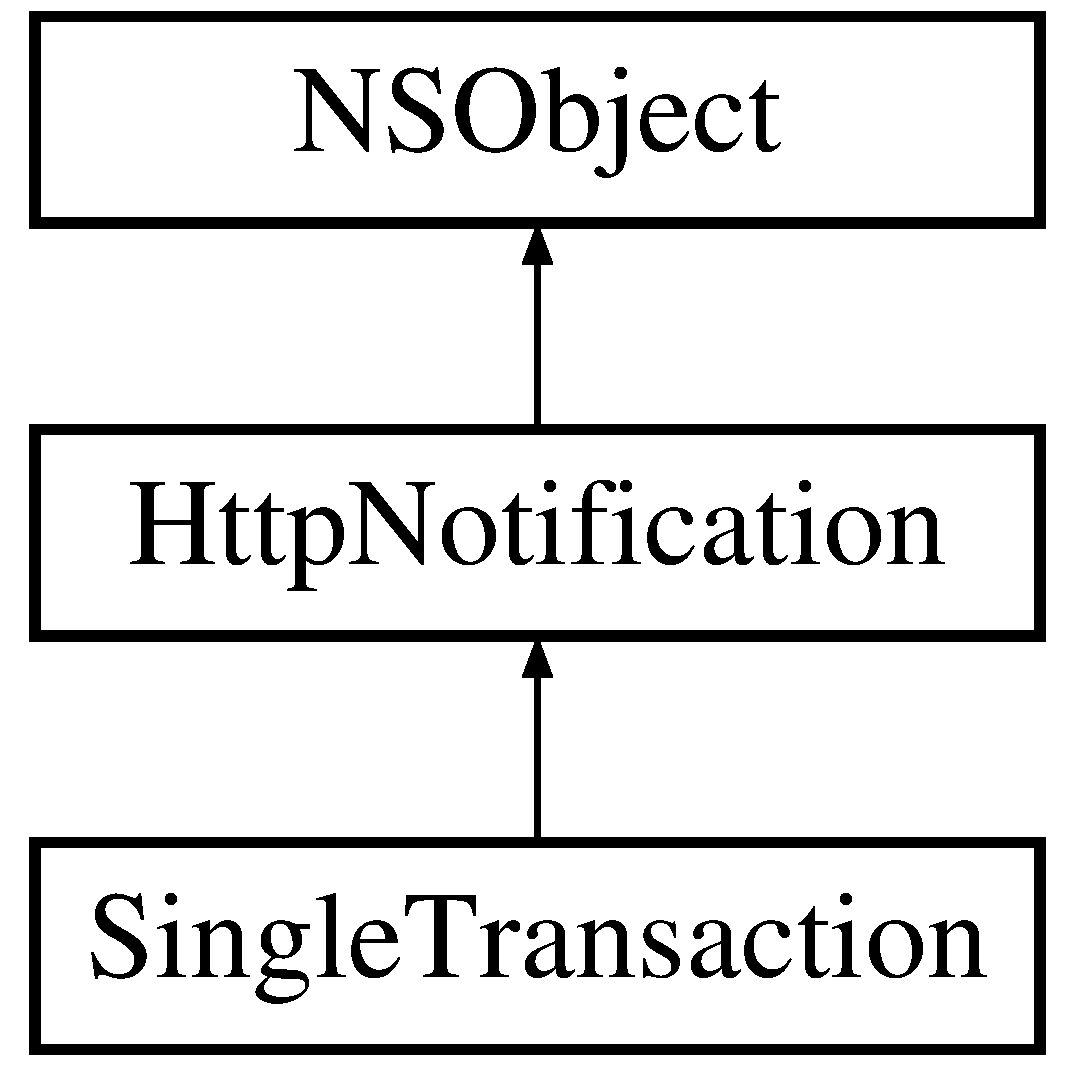
\includegraphics[height=3.000000cm]{interface_http_notification}
\end{center}
\end{figure}
\subsection*{Instance Methods}
\begin{DoxyCompactItemize}
\item 
\mbox{\Hypertarget{interface_http_notification_a19afbd02c594100357d5fba77f15171c}\label{interface_http_notification_a19afbd02c594100357d5fba77f15171c}} 
(id) -\/ {\bfseries init}
\item 
\mbox{\Hypertarget{interface_http_notification_a1988f3ada0558d7b2c61723675694382}\label{interface_http_notification_a1988f3ada0558d7b2c61723675694382}} 
(void) -\/ {\bfseries dealloc}
\end{DoxyCompactItemize}
\subsection*{Properties}
\begin{DoxyCompactItemize}
\item 
\mbox{\Hypertarget{interface_http_notification_a43218997491261c7346634cff04722cc}\label{interface_http_notification_a43218997491261c7346634cff04722cc}} 
N\+S\+String $\ast$ {\bfseries request\+Id}
\item 
\mbox{\Hypertarget{interface_http_notification_a46b15249aea6cbfc738d9e710d75a115}\label{interface_http_notification_a46b15249aea6cbfc738d9e710d75a115}} 
N\+S\+String $\ast$ {\bfseries host}
\item 
\mbox{\Hypertarget{interface_http_notification_ab13994fda2459c0e7c1921897e0e6eca}\label{interface_http_notification_ab13994fda2459c0e7c1921897e0e6eca}} 
N\+S\+String $\ast$ {\bfseries scheme}
\item 
\mbox{\Hypertarget{interface_http_notification_a8d1cd130ec125944e62267419b2d3fe7}\label{interface_http_notification_a8d1cd130ec125944e62267419b2d3fe7}} 
\hyperlink{interface_http_request_model}{Http\+Request\+Model} $\ast$ {\bfseries request}
\item 
\mbox{\Hypertarget{interface_http_notification_affc5114b35502c34dc92b9a21308eb33}\label{interface_http_notification_affc5114b35502c34dc92b9a21308eb33}} 
\hyperlink{interface_http_response_model}{Http\+Response\+Model} $\ast$ {\bfseries response}
\end{DoxyCompactItemize}


The documentation for this class was generated from the following files\+:\begin{DoxyCompactItemize}
\item 
marvin/objc/http\+\_\+notification.\+h\item 
marvin/objc/http\+\_\+notification.\+mm\end{DoxyCompactItemize}

\hypertarget{interface_http_request_model}{}\section{Http\+Request\+Model Class Reference}
\label{interface_http_request_model}\index{Http\+Request\+Model@{Http\+Request\+Model}}
Inheritance diagram for Http\+Request\+Model\+:\begin{figure}[H]
\begin{center}
\leavevmode
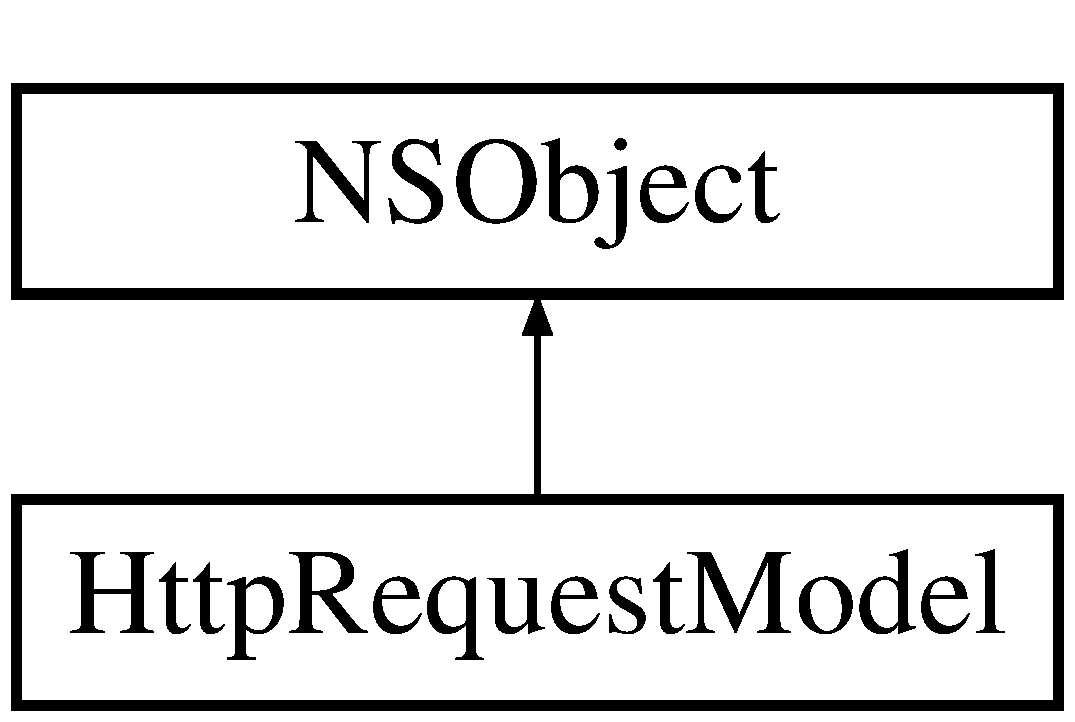
\includegraphics[height=2.000000cm]{interface_http_request_model}
\end{center}
\end{figure}
\subsection*{Instance Methods}
\begin{DoxyCompactItemize}
\item 
\mbox{\Hypertarget{interface_http_request_model_a467c64d1c09b7a114cf88878cadf2dc9}\label{interface_http_request_model_a467c64d1c09b7a114cf88878cadf2dc9}} 
(id) -\/ {\bfseries init}
\item 
\mbox{\Hypertarget{interface_http_request_model_aedbaf1e4759d2bd4f835ce28e5ae84f3}\label{interface_http_request_model_aedbaf1e4759d2bd4f835ce28e5ae84f3}} 
(void) -\/ {\bfseries dealloc}
\end{DoxyCompactItemize}
\subsection*{Properties}
\begin{DoxyCompactItemize}
\item 
\mbox{\Hypertarget{interface_http_request_model_acdb84a5d51dc3ac247b78c9092d9d391}\label{interface_http_request_model_acdb84a5d51dc3ac247b78c9092d9d391}} 
N\+S\+Number $\ast$ {\bfseries minor\+Version}
\item 
\mbox{\Hypertarget{interface_http_request_model_af33b88fdfa37408c34e6bcd645322c8b}\label{interface_http_request_model_af33b88fdfa37408c34e6bcd645322c8b}} 
N\+S\+Number $\ast$ {\bfseries method}
\item 
\mbox{\Hypertarget{interface_http_request_model_afcf7ec9a72dbfe5ff47a695a02252cf9}\label{interface_http_request_model_afcf7ec9a72dbfe5ff47a695a02252cf9}} 
N\+S\+String $\ast$ {\bfseries method\+Str}
\item 
\mbox{\Hypertarget{interface_http_request_model_add189cd0330b0b619a959c44cf642351}\label{interface_http_request_model_add189cd0330b0b619a959c44cf642351}} 
N\+S\+String $\ast$ {\bfseries uri}
\item 
\mbox{\Hypertarget{interface_http_request_model_a39993585a1bb2a4f150f3fb05bc8707b}\label{interface_http_request_model_a39993585a1bb2a4f150f3fb05bc8707b}} 
N\+S\+String $\ast$ {\bfseries headers}
\item 
\mbox{\Hypertarget{interface_http_request_model_aa2ef33396ca26ceef8655f73d3e4ab53}\label{interface_http_request_model_aa2ef33396ca26ceef8655f73d3e4ab53}} 
N\+S\+String $\ast$ {\bfseries body}
\end{DoxyCompactItemize}


The documentation for this class was generated from the following files\+:\begin{DoxyCompactItemize}
\item 
marvin/objc/http\+\_\+request\+\_\+model.\+h\item 
marvin/objc/http\+\_\+request\+\_\+model.\+mm\end{DoxyCompactItemize}

\hypertarget{interface_http_response_model}{}\section{Http\+Response\+Model Class Reference}
\label{interface_http_response_model}\index{Http\+Response\+Model@{Http\+Response\+Model}}
Inheritance diagram for Http\+Response\+Model\+:\begin{figure}[H]
\begin{center}
\leavevmode
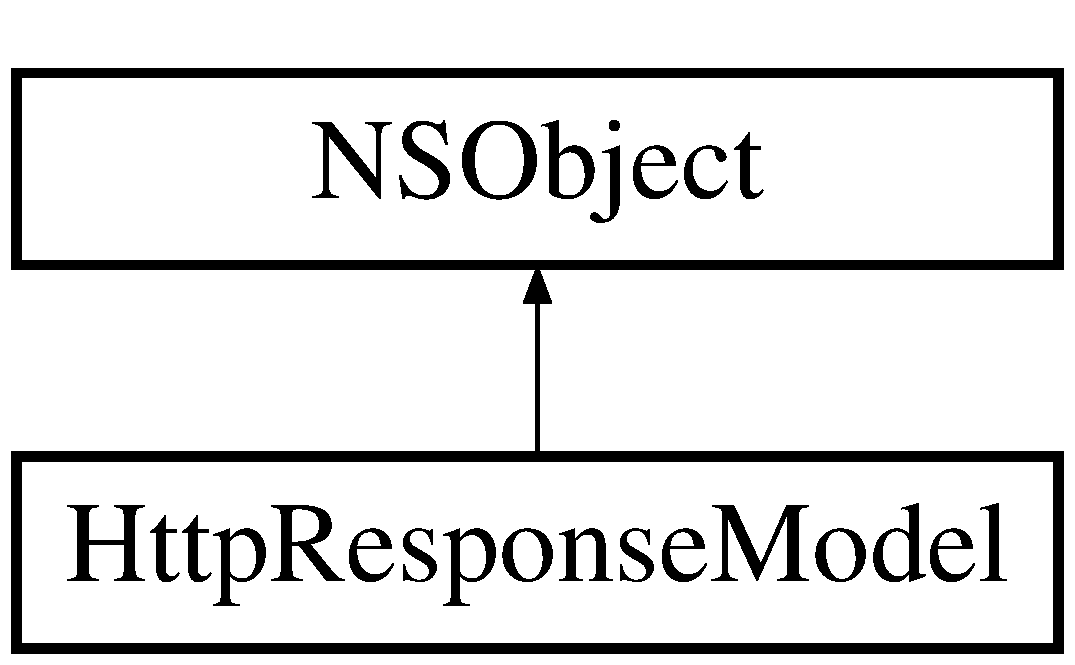
\includegraphics[height=2.000000cm]{interface_http_response_model}
\end{center}
\end{figure}
\subsection*{Instance Methods}
\begin{DoxyCompactItemize}
\item 
\mbox{\Hypertarget{interface_http_response_model_a1a6f6c00d479c20577c40bdb0c216cd3}\label{interface_http_response_model_a1a6f6c00d479c20577c40bdb0c216cd3}} 
(id) -\/ {\bfseries init}
\item 
\mbox{\Hypertarget{interface_http_response_model_a3b049ae6a70dce98f47c8662639a4048}\label{interface_http_response_model_a3b049ae6a70dce98f47c8662639a4048}} 
(void) -\/ {\bfseries dealloc}
\end{DoxyCompactItemize}
\subsection*{Properties}
\begin{DoxyCompactItemize}
\item 
\mbox{\Hypertarget{interface_http_response_model_adea16f6b694f3a367a9092e6aad5d715}\label{interface_http_response_model_adea16f6b694f3a367a9092e6aad5d715}} 
N\+S\+Number $\ast$ {\bfseries minor\+Version}
\item 
\mbox{\Hypertarget{interface_http_response_model_ac7afa813b63b28639461532b5e374caf}\label{interface_http_response_model_ac7afa813b63b28639461532b5e374caf}} 
N\+S\+Number $\ast$ {\bfseries status\+Code}
\item 
\mbox{\Hypertarget{interface_http_response_model_a79213ed7274523c0377c136e726f1536}\label{interface_http_response_model_a79213ed7274523c0377c136e726f1536}} 
N\+S\+String $\ast$ {\bfseries status}
\item 
\mbox{\Hypertarget{interface_http_response_model_a14f455063378dcf126ae1be299634e90}\label{interface_http_response_model_a14f455063378dcf126ae1be299634e90}} 
N\+S\+String $\ast$ {\bfseries headers}
\item 
\mbox{\Hypertarget{interface_http_response_model_ad30b96c99f691733c69a13fa01dd06d3}\label{interface_http_response_model_ad30b96c99f691733c69a13fa01dd06d3}} 
N\+S\+String $\ast$ {\bfseries body}
\end{DoxyCompactItemize}


The documentation for this class was generated from the following files\+:\begin{DoxyCompactItemize}
\item 
marvin/objc/http\+\_\+response\+\_\+model.\+h\item 
marvin/objc/http\+\_\+response\+\_\+model.\+mm\end{DoxyCompactItemize}

\hypertarget{class_h_t_t_p_server}{}\section{H\+T\+T\+P\+Server Class Reference}
\label{class_h_t_t_p_server}\index{H\+T\+T\+P\+Server@{H\+T\+T\+P\+Server}}


H\+T\+TP server class.  T\+Request\+Handler is a template argument that must conform to \hyperlink{class_request_handler_base}{Request\+Handler\+Base} for a class that will handle an http request and send the necessary response.  




{\ttfamily \#include $<$http\+\_\+server.\+hpp$>$}

\subsection*{Public Member Functions}
\begin{DoxyCompactItemize}
\item 
\mbox{\Hypertarget{class_h_t_t_p_server_a3ccc2f74d6b566df84a08155a81dbf33}\label{class_h_t_t_p_server_a3ccc2f74d6b566df84a08155a81dbf33}} 
{\bfseries H\+T\+T\+P\+Server} (const \hyperlink{class_h_t_t_p_server}{H\+T\+T\+P\+Server} \&)=delete
\item 
\mbox{\Hypertarget{class_h_t_t_p_server_af0ff3249ee7308563225f0470f449ead}\label{class_h_t_t_p_server_af0ff3249ee7308563225f0470f449ead}} 
\hyperlink{class_h_t_t_p_server}{H\+T\+T\+P\+Server} \& {\bfseries operator=} (const \hyperlink{class_h_t_t_p_server}{H\+T\+T\+P\+Server} \&)=delete
\item 
\hyperlink{class_h_t_t_p_server_a5a5f52fff7b98136607a692aa06d8ba4}{H\+T\+T\+P\+Server} (Request\+Handler\+Factory factory)
\begin{DoxyCompactList}\small\item\em Construct the server to listen on the specified T\+CP address and port. \end{DoxyCompactList}\item 
\mbox{\Hypertarget{class_h_t_t_p_server_aece3ed957213b41813b5eafff259ad9d}\label{class_h_t_t_p_server_aece3ed957213b41813b5eafff259ad9d}} 
void \hyperlink{class_h_t_t_p_server_aece3ed957213b41813b5eafff259ad9d}{listen} (long port=9991)
\begin{DoxyCompactList}\small\item\em starts the listen process on the servers port, and from there dispatches instances of T\+Request\+Handler to service the connection \end{DoxyCompactList}\item 
\mbox{\Hypertarget{class_h_t_t_p_server_a263a0e7cedafc3def65be6278e894dbc}\label{class_h_t_t_p_server_a263a0e7cedafc3def65be6278e894dbc}} 
void {\bfseries terminate} ()
\end{DoxyCompactItemize}
\subsection*{Static Public Member Functions}
\begin{DoxyCompactItemize}
\item 
static bool \hyperlink{class_h_t_t_p_server_a903d110951861510bd885333ee22fb6c}{verify} ()
\item 
\mbox{\Hypertarget{class_h_t_t_p_server_acd4c031485802323ff872b76860413bf}\label{class_h_t_t_p_server_acd4c031485802323ff872b76860413bf}} 
static void {\bfseries config\+Set\+\_\+\+Number\+Of\+Connections} (int num)
\item 
\mbox{\Hypertarget{class_h_t_t_p_server_adcf739f3cd5e055c0155ec6bc3cd9cc6}\label{class_h_t_t_p_server_adcf739f3cd5e055c0155ec6bc3cd9cc6}} 
static void {\bfseries config\+Set\+\_\+\+Number\+Of\+Threads} (int num)
\item 
\mbox{\Hypertarget{class_h_t_t_p_server_ab9f39cb7b348bb1bcd3a671bd2706b57}\label{class_h_t_t_p_server_ab9f39cb7b348bb1bcd3a671bd2706b57}} 
static void {\bfseries config\+Set\+\_\+\+Heartbeat\+Interval} (int millisecs)
\item 
\mbox{\Hypertarget{class_h_t_t_p_server_a77afcf8dc54df4a24cdf7a1bd2d29aaf}\label{class_h_t_t_p_server_a77afcf8dc54df4a24cdf7a1bd2d29aaf}} 
static \hyperlink{class_h_t_t_p_server}{H\+T\+T\+P\+Server} $\ast$ {\bfseries get\+\_\+instance} ()
\end{DoxyCompactItemize}


\subsection{Detailed Description}
H\+T\+TP server class.  T\+Request\+Handler is a template argument that must conform to \hyperlink{class_request_handler_base}{Request\+Handler\+Base} for a class that will handle an http request and send the necessary response. 

Discussion of structure

T\+Request\+Handler is a \char`\"{}user\char`\"{} provided class instance that actually handles a one or more request on a single connection.

connection\+\_\+handler (\hyperlink{class_connection_handler}{Connection\+Handler}) wraps a single instance of T\+Request\+Handler and manages the life cycle of that T\+Request\+Handler instance, and thus represents the life time of a single client connection.

server\+\_\+connection\+\_\+manager (\hyperlink{class_server_connection_manager}{Server\+Connection\+Manager})
\begin{DoxyItemize}
\item only one of these exists. That instance
\item keeps track of a smart pointer to every active instane of \hyperlink{class_connection_handler}{Connection\+Handler} thereby ensures they stay in existence while active and can be deleted en-\/mass if/when the server needs to close down
\item limits the number of active \hyperlink{class_connection_handler}{Connection\+Handler} instances at any point in time to ensure that the server does not get overloaded. 
\end{DoxyItemize}

\subsection{Constructor \& Destructor Documentation}
\mbox{\Hypertarget{class_h_t_t_p_server_a5a5f52fff7b98136607a692aa06d8ba4}\label{class_h_t_t_p_server_a5a5f52fff7b98136607a692aa06d8ba4}} 
\index{H\+T\+T\+P\+Server@{H\+T\+T\+P\+Server}!H\+T\+T\+P\+Server@{H\+T\+T\+P\+Server}}
\index{H\+T\+T\+P\+Server@{H\+T\+T\+P\+Server}!H\+T\+T\+P\+Server@{H\+T\+T\+P\+Server}}
\subsubsection{\texorpdfstring{H\+T\+T\+P\+Server()}{HTTPServer()}}
{\footnotesize\ttfamily H\+T\+T\+P\+Server\+::\+H\+T\+T\+P\+Server (\begin{DoxyParamCaption}\item[{Request\+Handler\+Factory}]{factory }\end{DoxyParamCaption})\hspace{0.3cm}{\ttfamily [explicit]}}



Construct the server to listen on the specified T\+CP address and port. 


\begin{DoxyParams}{Parameters}
{\em long} & port defaults to 9991 \\
\hline
\end{DoxyParams}


\subsection{Member Function Documentation}
\mbox{\Hypertarget{class_h_t_t_p_server_a903d110951861510bd885333ee22fb6c}\label{class_h_t_t_p_server_a903d110951861510bd885333ee22fb6c}} 
\index{H\+T\+T\+P\+Server@{H\+T\+T\+P\+Server}!verify@{verify}}
\index{verify@{verify}!H\+T\+T\+P\+Server@{H\+T\+T\+P\+Server}}
\subsubsection{\texorpdfstring{verify()}{verify()}}
{\footnotesize\ttfamily bool H\+T\+T\+P\+Server\+::verify (\begin{DoxyParamCaption}{ }\end{DoxyParamCaption})\hspace{0.3cm}{\ttfamily [static]}}

This is for testing only and should be called after all clients have finished to verify that all connections are closed, all connection handlers have been deleted and all sockets are freed up 

The documentation for this class was generated from the following files\+:\begin{DoxyCompactItemize}
\item 
marvin/server/http\+\_\+server.\+hpp\item 
marvin/server/http\+\_\+server.\+cpp\end{DoxyCompactItemize}

\hypertarget{class_in_use_connections_type}{}\section{In\+Use\+Connections\+Type Class Reference}
\label{class_in_use_connections_type}\index{In\+Use\+Connections\+Type@{In\+Use\+Connections\+Type}}
\subsection*{Public Member Functions}
\begin{DoxyCompactItemize}
\item 
\mbox{\Hypertarget{class_in_use_connections_type_a0dc7ed043e59287fac24b3828dcd5ec6}\label{class_in_use_connections_type_a0dc7ed043e59287fac24b3828dcd5ec6}} 
std\+::size\+\_\+t {\bfseries size} ()
\item 
\mbox{\Hypertarget{class_in_use_connections_type_a70a45d1639a736696231e44cb60df098}\label{class_in_use_connections_type_a70a45d1639a736696231e44cb60df098}} 
void {\bfseries remove} (\hyperlink{class_connection_interface}{Connection\+Interface} $\ast$a\+Conn)
\item 
\mbox{\Hypertarget{class_in_use_connections_type_a357a86a5de5b8c606f25870d636b0027}\label{class_in_use_connections_type_a357a86a5de5b8c606f25870d636b0027}} 
void {\bfseries add} (\hyperlink{class_connection_interface}{Connection\+Interface} $\ast$conn)
\item 
\mbox{\Hypertarget{class_in_use_connections_type_a0dc7ed043e59287fac24b3828dcd5ec6}\label{class_in_use_connections_type_a0dc7ed043e59287fac24b3828dcd5ec6}} 
std\+::size\+\_\+t {\bfseries size} ()
\item 
\mbox{\Hypertarget{class_in_use_connections_type_a70a45d1639a736696231e44cb60df098}\label{class_in_use_connections_type_a70a45d1639a736696231e44cb60df098}} 
void {\bfseries remove} (\hyperlink{class_connection_interface}{Connection\+Interface} $\ast$a\+Conn)
\item 
\mbox{\Hypertarget{class_in_use_connections_type_a357a86a5de5b8c606f25870d636b0027}\label{class_in_use_connections_type_a357a86a5de5b8c606f25870d636b0027}} 
void {\bfseries add} (\hyperlink{class_connection_interface}{Connection\+Interface} $\ast$conn)
\item 
\mbox{\Hypertarget{class_in_use_connections_type_a62e83cf6e070093e56e1fe1c3bd21fda}\label{class_in_use_connections_type_a62e83cf6e070093e56e1fe1c3bd21fda}} 
{\bfseries In\+Use\+Connections} (boost\+::asio\+::io\+\_\+service \&io)
\item 
\mbox{\Hypertarget{class_in_use_connections_type_a0dc7ed043e59287fac24b3828dcd5ec6}\label{class_in_use_connections_type_a0dc7ed043e59287fac24b3828dcd5ec6}} 
std\+::size\+\_\+t {\bfseries size} ()
\item 
\mbox{\Hypertarget{class_in_use_connections_type_a3a12406ec1666fe7d0c53391b2cba2b3}\label{class_in_use_connections_type_a3a12406ec1666fe7d0c53391b2cba2b3}} 
void {\bfseries remove} (\hyperlink{class_assigned_connection}{Assigned\+Connection} $\ast$a\+Conn)
\item 
\mbox{\Hypertarget{class_in_use_connections_type_a36211f9768a4d78a1cd1f9fa4d861420}\label{class_in_use_connections_type_a36211f9768a4d78a1cd1f9fa4d861420}} 
void {\bfseries add} (\hyperlink{class_assigned_connection}{Assigned\+Connection} $\ast$conn)
\end{DoxyCompactItemize}


The documentation for this class was generated from the following files\+:\begin{DoxyCompactItemize}
\item 
marvin/connection/connection\+\_\+pool.\+hpp\item 
marvin/server/connection\+\_\+handler\+\_\+pool.\+hpp\item 
marvin/src/connection\+\_\+pool copy.\+cpp\item 
marvin/connection/connection\+\_\+pool.\+cpp\item 
marvin/server/connection\+\_\+handler\+\_\+pool .\+cpp\end{DoxyCompactItemize}

\hypertarget{structboost_1_1system_1_1is__error__code__enum_3_01_marvin_1_1errc_01_4}{}\section{boost\+:\+:system\+:\+:is\+\_\+error\+\_\+code\+\_\+enum$<$ Marvin\+:\+:errc $>$ Struct Template Reference}
\label{structboost_1_1system_1_1is__error__code__enum_3_01_marvin_1_1errc_01_4}\index{boost\+::system\+::is\+\_\+error\+\_\+code\+\_\+enum$<$ Marvin\+::errc $>$@{boost\+::system\+::is\+\_\+error\+\_\+code\+\_\+enum$<$ Marvin\+::errc $>$}}
Inheritance diagram for boost\+:\+:system\+:\+:is\+\_\+error\+\_\+code\+\_\+enum$<$ Marvin\+:\+:errc $>$\+:\begin{figure}[H]
\begin{center}
\leavevmode
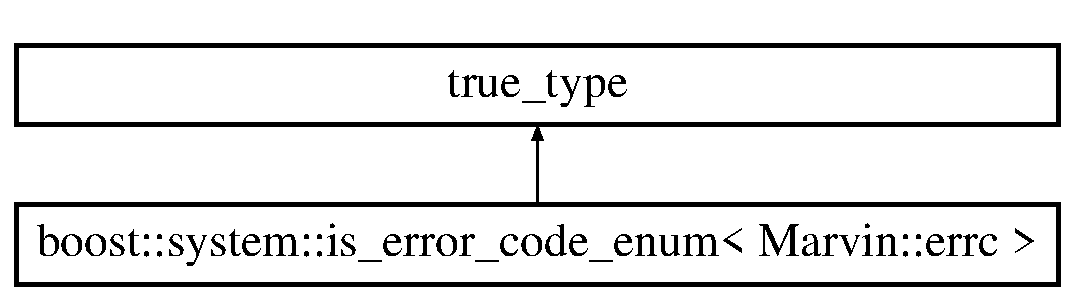
\includegraphics[height=2.000000cm]{structboost_1_1system_1_1is__error__code__enum_3_01_marvin_1_1errc_01_4}
\end{center}
\end{figure}


The documentation for this struct was generated from the following file\+:\begin{DoxyCompactItemize}
\item 
marvin/error/marvin\+\_\+error.\+hpp\end{DoxyCompactItemize}

\hypertarget{protocol_marvin_delegate-p}{}\section{$<$Marvin\+Delegate$>$ Protocol Reference}
\label{protocol_marvin_delegate-p}\index{$<$\+Marvin\+Delegate$>$@{$<$\+Marvin\+Delegate$>$}}


{\ttfamily \#import $<$marvin\+\_\+objc.\+h$>$}

\subsection*{Instance Methods}
\begin{DoxyCompactItemize}
\item 
\mbox{\Hypertarget{protocol_marvin_delegate-p_a0d53e9f0e09747b53ecbde78e3effac3}\label{protocol_marvin_delegate-p_a0d53e9f0e09747b53ecbde78e3effac3}} 
(void) -\/ {\bfseries notify\+:}
\end{DoxyCompactItemize}


\subsection{Detailed Description}
This class is a wrapper around the c/c++ implementation of the marvin proxy 

The documentation for this protocol was generated from the following file\+:\begin{DoxyCompactItemize}
\item 
marvin/objc/marvin\+\_\+objc.\+h\end{DoxyCompactItemize}

\hypertarget{interface_marvin_delegate_objc}{}\section{Marvin\+Delegate\+Objc Class Reference}
\label{interface_marvin_delegate_objc}\index{Marvin\+Delegate\+Objc@{Marvin\+Delegate\+Objc}}


{\ttfamily \#import $<$marvin\+\_\+delegate\+\_\+objc.\+h$>$}

Inheritance diagram for Marvin\+Delegate\+Objc\+:\begin{figure}[H]
\begin{center}
\leavevmode
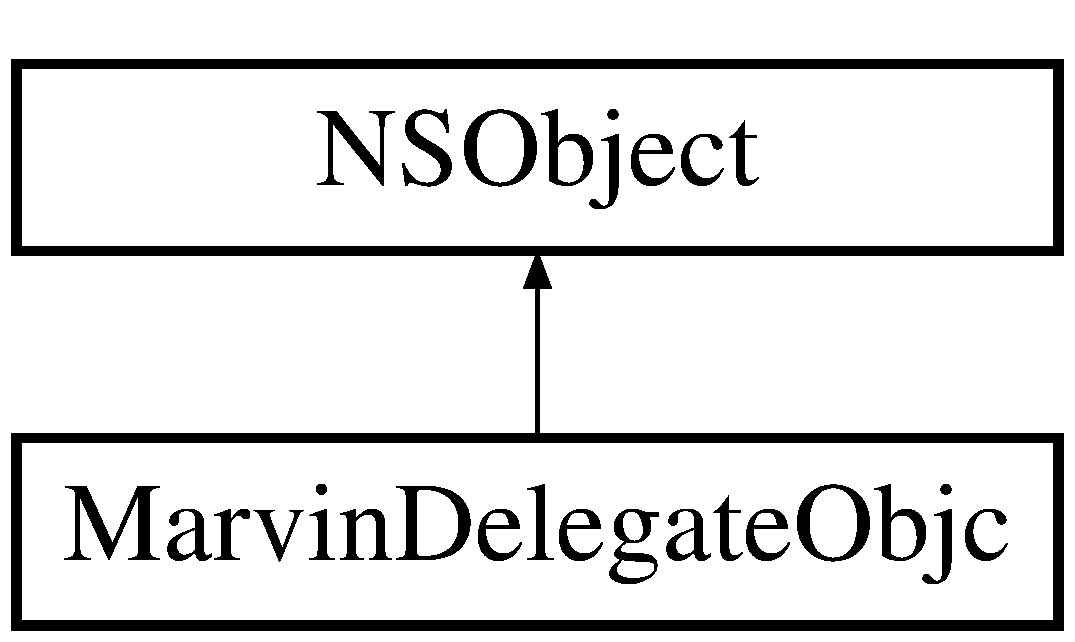
\includegraphics[height=2.000000cm]{interface_marvin_delegate_objc}
\end{center}
\end{figure}
\subsection*{Instance Methods}
\begin{DoxyCompactItemize}
\item 
(id) -\/ {\bfseries init}
\item 
\mbox{\Hypertarget{interface_marvin_delegate_objc_a4cc278c4868c917f1cc99d050bfad22e}\label{interface_marvin_delegate_objc_a4cc278c4868c917f1cc99d050bfad22e}} 
(void) -\/ {\bfseries set\+Captured\+Traffic\+:}
\item 
\mbox{\Hypertarget{interface_marvin_delegate_objc_a24f5f03152b92b30ed617b8552c26933}\label{interface_marvin_delegate_objc_a24f5f03152b92b30ed617b8552c26933}} 
(void) -\/ {\bfseries notify\+:}
\end{DoxyCompactItemize}


\subsection{Detailed Description}
This is an example class, that shows how to get notification of http transactions from the \hyperlink{namespace_marvin}{Marvin} proxy 

\subsection{Method Documentation}
\mbox{\Hypertarget{interface_marvin_delegate_objc_a6e02c2ba9e32968e72046c6f538d310f}\label{interface_marvin_delegate_objc_a6e02c2ba9e32968e72046c6f538d310f}} 
\index{Marvin\+Delegate\+Objc@{Marvin\+Delegate\+Objc}!init@{init}}
\index{init@{init}!Marvin\+Delegate\+Objc@{Marvin\+Delegate\+Objc}}
\subsubsection{\texorpdfstring{init()}{init()}}
{\footnotesize\ttfamily -\/ (id) init \begin{DoxyParamCaption}{ }\end{DoxyParamCaption}}

{\bfseries Initial value\+:}
\begin{DoxyCode}
\{
    \hyperlink{interface_captured_traffic}{CapturedTraffic}* \_capturedTraffic
\end{DoxyCode}


The documentation for this class was generated from the following files\+:\begin{DoxyCompactItemize}
\item 
marvin/objc/marvin\+\_\+delegate\+\_\+objc.\+h\item 
marvin/objc/marvin\+\_\+delegate\+\_\+objc.\+mm\end{DoxyCompactItemize}

\hypertarget{interface_marvin_obj}{}\section{Marvin\+Obj Class Reference}
\label{interface_marvin_obj}\index{Marvin\+Obj@{Marvin\+Obj}}
Inheritance diagram for Marvin\+Obj\+:\begin{figure}[H]
\begin{center}
\leavevmode
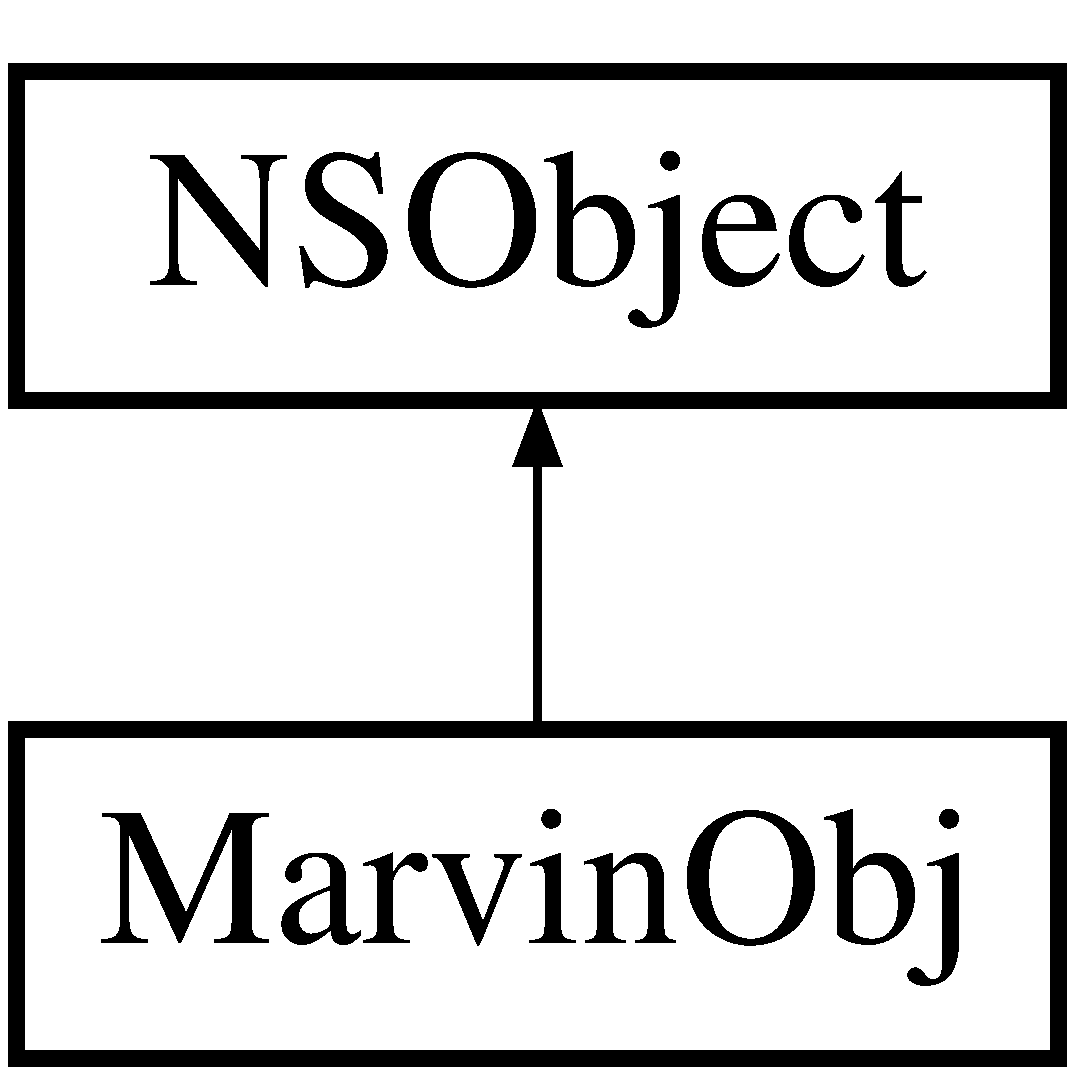
\includegraphics[height=2.000000cm]{interface_marvin_obj}
\end{center}
\end{figure}
\subsection*{Instance Methods}
\begin{DoxyCompactItemize}
\item 
\mbox{\Hypertarget{interface_marvin_obj_a7b93b5ebbd36b83ac6264f5b024ed5cc}\label{interface_marvin_obj_a7b93b5ebbd36b83ac6264f5b024ed5cc}} 
(void) -\/ {\bfseries run}
\end{DoxyCompactItemize}


The documentation for this class was generated from the following file\+:\begin{DoxyCompactItemize}
\item 
marvin/objc/marvin\+\_\+objc.\+mm\end{DoxyCompactItemize}

\hypertarget{interface_marvin_objc}{}\section{Marvin\+Objc Class Reference}
\label{interface_marvin_objc}\index{Marvin\+Objc@{Marvin\+Objc}}
Inheritance diagram for Marvin\+Objc\+:\begin{figure}[H]
\begin{center}
\leavevmode
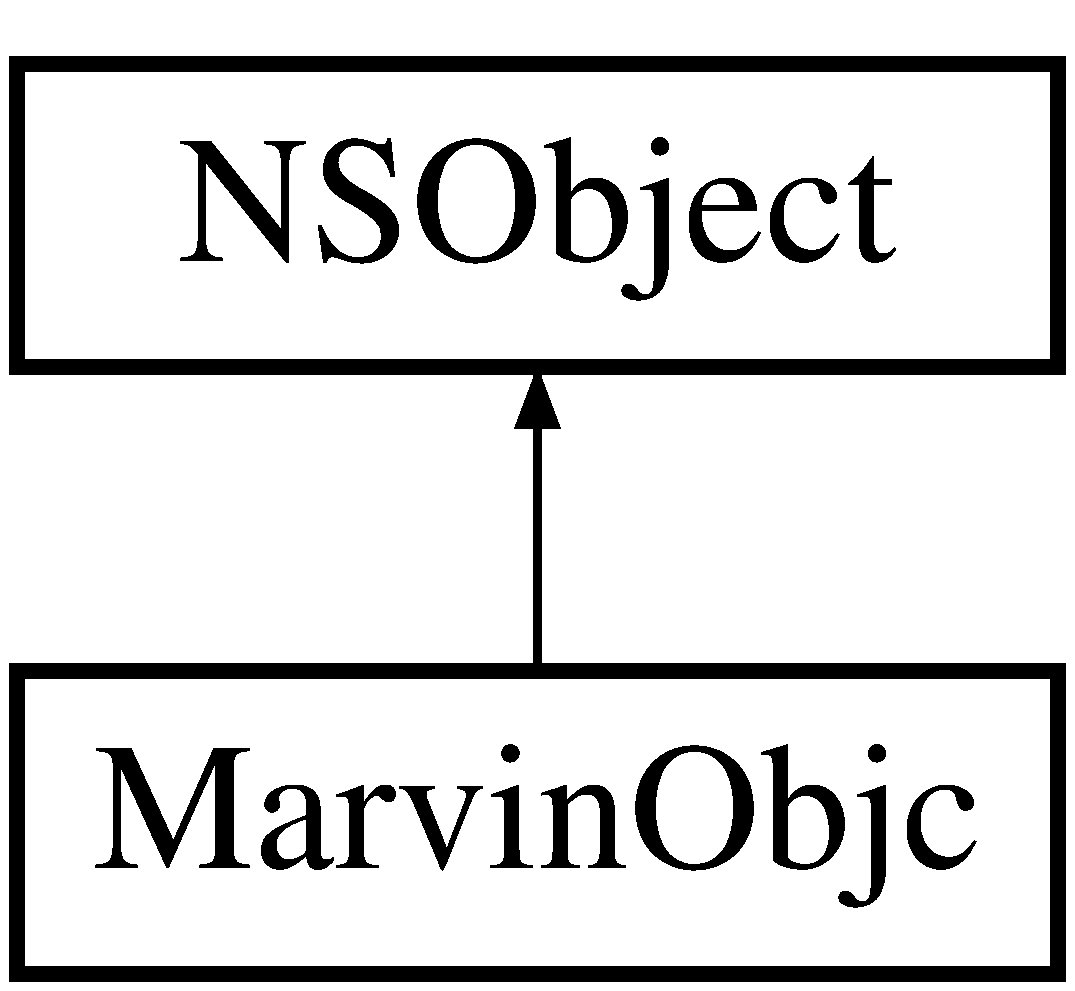
\includegraphics[height=2.000000cm]{interface_marvin_objc}
\end{center}
\end{figure}
\subsection*{Instance Methods}
\begin{DoxyCompactItemize}
\item 
(void) -\/ \hyperlink{interface_marvin_objc_a5f10e6ef563d08e6a7ef1fcb9495b36f}{start}
\item 
\mbox{\Hypertarget{interface_marvin_objc_aa0525a6aed868a4821768b9131ae5412}\label{interface_marvin_objc_aa0525a6aed868a4821768b9131ae5412}} 
(void) -\/ {\bfseries set\+Delegate\+:}
\item 
\mbox{\Hypertarget{interface_marvin_objc_a49d1fa6327a38fa34e35566499e6058f}\label{interface_marvin_objc_a49d1fa6327a38fa34e35566499e6058f}} 
(void) -\/ {\bfseries set\+Port\+:}
\end{DoxyCompactItemize}


\subsection{Method Documentation}
\mbox{\Hypertarget{interface_marvin_objc_a5f10e6ef563d08e6a7ef1fcb9495b36f}\label{interface_marvin_objc_a5f10e6ef563d08e6a7ef1fcb9495b36f}} 
\index{Marvin\+Objc@{Marvin\+Objc}!start@{start}}
\index{start@{start}!Marvin\+Objc@{Marvin\+Objc}}
\subsubsection{\texorpdfstring{start()}{start()}}
{\footnotesize\ttfamily -\/ (void) start \begin{DoxyParamCaption}{ }\end{DoxyParamCaption}}

Starts the \hyperlink{namespace_marvin}{Marvin} proxy on a background thread so that boost can manage its own run loop 

The documentation for this class was generated from the following files\+:\begin{DoxyCompactItemize}
\item 
marvin/objc/marvin\+\_\+objc.\+h\item 
marvin/objc/marvin\+\_\+objc.\+mm\end{DoxyCompactItemize}

\hypertarget{struct_m_buffer}{}\section{M\+Buffer Struct Reference}
\label{struct_m_buffer}\index{M\+Buffer@{M\+Buffer}}


\hyperlink{struct_m_buffer}{M\+Buffer} a contiguous buffer.  




{\ttfamily \#include $<$buffer.\+hpp$>$}

\subsection*{Public Member Functions}
\begin{DoxyCompactItemize}
\item 
\hyperlink{struct_m_buffer_a4f12e1ae3dc9acf4739f4cb8df49cb98}{M\+Buffer} (const std\+::size\+\_\+t cap)
\item 
\hyperlink{struct_m_buffer_a7afd94b5e8b2a26ffab8ede1aef06f07}{$\sim$\+M\+Buffer} ()
\item 
void $\ast$ \hyperlink{struct_m_buffer_a76fda1089c0abb54ac72977228245725}{data} ()
\item 
std\+::size\+\_\+t \hyperlink{struct_m_buffer_a9b3db2bdbcadcb68478cc5edc6164432}{size} ()
\item 
std\+::size\+\_\+t \hyperlink{struct_m_buffer_acadde0f7cb85b05602a61aa8e3277369}{capacity} ()
\item 
void $\ast$ \hyperlink{struct_m_buffer_a3a520754e8335f75136135caea741960}{next\+Available} ()
\item 
\hyperlink{struct_m_buffer}{M\+Buffer} \& \hyperlink{struct_m_buffer_a6b1a469848174ab1925e964034408c07}{empty} ()
\item 
\hyperlink{struct_m_buffer}{M\+Buffer} \& \hyperlink{struct_m_buffer_abb2765e8b761bbd0c17fdd7bdaada053}{append} (void $\ast$\hyperlink{struct_m_buffer_a76fda1089c0abb54ac72977228245725}{data}, std\+::size\+\_\+t len)
\item 
\mbox{\Hypertarget{struct_m_buffer_a29b005cac5a7d2a7690145e8c3121e6f}\label{struct_m_buffer_a29b005cac5a7d2a7690145e8c3121e6f}} 
\hyperlink{struct_m_buffer}{M\+Buffer} \& {\bfseries set\+Size} (std\+::size\+\_\+t n)
\item 
std\+::string \hyperlink{struct_m_buffer_af3600a4125123ee2b0e62fb84fd758a0}{to\+String} ()
\item 
bool \hyperlink{struct_m_buffer_a629f84798448ae301df28d3d54520135}{contains} (void $\ast$ptr)
\item 
\mbox{\Hypertarget{struct_m_buffer_ae84bf1ea3e993bef7967ea4685fd8adc}\label{struct_m_buffer_ae84bf1ea3e993bef7967ea4685fd8adc}} 
bool {\bfseries contains} (char $\ast$ptr)
\end{DoxyCompactItemize}
\subsection*{Protected Attributes}
\begin{DoxyCompactItemize}
\item 
\mbox{\Hypertarget{struct_m_buffer_ae9f75c8701f5cae42b8384ae4edb1ad1}\label{struct_m_buffer_ae9f75c8701f5cae42b8384ae4edb1ad1}} 
void $\ast$ {\bfseries mem\+Ptr}
\item 
\mbox{\Hypertarget{struct_m_buffer_a508d55df27bae34cd8ed486c0b226ab1}\label{struct_m_buffer_a508d55df27bae34cd8ed486c0b226ab1}} 
char $\ast$ \hyperlink{struct_m_buffer_a508d55df27bae34cd8ed486c0b226ab1}{c\+Ptr}
\begin{DoxyCompactList}\small\item\em points to the start of the memory slab managed by the instance \end{DoxyCompactList}\item 
\mbox{\Hypertarget{struct_m_buffer_a98d22bf882aa625b6cf24cfc2f34be5e}\label{struct_m_buffer_a98d22bf882aa625b6cf24cfc2f34be5e}} 
std\+::size\+\_\+t \hyperlink{struct_m_buffer_a98d22bf882aa625b6cf24cfc2f34be5e}{length\+\_\+}
\begin{DoxyCompactList}\small\item\em same as mem\+Ptr but makes it easier in debugger to see whats in the buffer \end{DoxyCompactList}\item 
\mbox{\Hypertarget{struct_m_buffer_a69e539d29403f2c50eec2cf75819549e}\label{struct_m_buffer_a69e539d29403f2c50eec2cf75819549e}} 
std\+::size\+\_\+t {\bfseries capacity\+\_\+}
\item 
\mbox{\Hypertarget{struct_m_buffer_a6e6bea091fb15983fd4f36a51150cabf}\label{struct_m_buffer_a6e6bea091fb15983fd4f36a51150cabf}} 
std\+::size\+\_\+t \hyperlink{struct_m_buffer_a6e6bea091fb15983fd4f36a51150cabf}{size\+\_\+}
\begin{DoxyCompactList}\small\item\em the capacity of the buffer, the value used for the malloc call \end{DoxyCompactList}\end{DoxyCompactItemize}
\subsection*{Friends}
\begin{DoxyCompactItemize}
\item 
boost\+::asio\+::const\+\_\+buffer \hyperlink{struct_m_buffer_a7c4fdebaff03d8d95c7915a9da1f8490}{mb\+\_\+as\+\_\+const\+\_\+buffer} (\hyperlink{struct_m_buffer}{M\+Buffer} \&bm)
\item 
boost\+::asio\+::mutable\+\_\+buffer \hyperlink{struct_m_buffer_a13c4f6e4208776d422e20509d873404d}{mb\+\_\+as\+\_\+mutable\+\_\+buffer} (\hyperlink{struct_m_buffer}{M\+Buffer} \&bm)
\item 
std\+::ostream \& \hyperlink{struct_m_buffer_abdaf184bb8d819d10f4676a9782e7bec}{operator$<$$<$} (std\+::ostream \&os, \hyperlink{struct_m_buffer}{M\+Buffer} \&b)
\end{DoxyCompactItemize}


\subsection{Detailed Description}
\hyperlink{struct_m_buffer}{M\+Buffer} a contiguous buffer. 

\hyperlink{struct_m_buffer}{M\+Buffer} class wraps a contigous buffer an provides manipulation methods. Once constructed the Mbuffer iinstance \char`\"{}own\char`\"{} the raw memory. \hyperlink{struct_m_buffer}{M\+Buffer} destructor releases the raw memory. 

\subsection{Constructor \& Destructor Documentation}
\mbox{\Hypertarget{struct_m_buffer_a4f12e1ae3dc9acf4739f4cb8df49cb98}\label{struct_m_buffer_a4f12e1ae3dc9acf4739f4cb8df49cb98}} 
\index{M\+Buffer@{M\+Buffer}!M\+Buffer@{M\+Buffer}}
\index{M\+Buffer@{M\+Buffer}!M\+Buffer@{M\+Buffer}}
\subsubsection{\texorpdfstring{M\+Buffer()}{MBuffer()}}
{\footnotesize\ttfamily M\+Buffer\+::\+M\+Buffer (\begin{DoxyParamCaption}\item[{const std\+::size\+\_\+t}]{cap }\end{DoxyParamCaption})}

Constructor -\/ give it a slab of memory to manage Let the \hyperlink{struct_m_buffer}{M\+Buffer} constructor allocate the memory -\/ but tell it howmuch \mbox{\Hypertarget{struct_m_buffer_a7afd94b5e8b2a26ffab8ede1aef06f07}\label{struct_m_buffer_a7afd94b5e8b2a26ffab8ede1aef06f07}} 
\index{M\+Buffer@{M\+Buffer}!````~M\+Buffer@{$\sim$\+M\+Buffer}}
\index{````~M\+Buffer@{$\sim$\+M\+Buffer}!M\+Buffer@{M\+Buffer}}
\subsubsection{\texorpdfstring{$\sim$\+M\+Buffer()}{~MBuffer()}}
{\footnotesize\ttfamily M\+Buffer\+::$\sim$\+M\+Buffer (\begin{DoxyParamCaption}{ }\end{DoxyParamCaption})}

destrtuctor -\/ frees the memory the instance is managing 

\subsection{Member Function Documentation}
\mbox{\Hypertarget{struct_m_buffer_abb2765e8b761bbd0c17fdd7bdaada053}\label{struct_m_buffer_abb2765e8b761bbd0c17fdd7bdaada053}} 
\index{M\+Buffer@{M\+Buffer}!append@{append}}
\index{append@{append}!M\+Buffer@{M\+Buffer}}
\subsubsection{\texorpdfstring{append()}{append()}}
{\footnotesize\ttfamily \hyperlink{struct_m_buffer}{M\+Buffer} \& M\+Buffer\+::append (\begin{DoxyParamCaption}\item[{void $\ast$}]{data,  }\item[{std\+::size\+\_\+t}]{len }\end{DoxyParamCaption})}

adds (by copying) data to the buffer starting at the first unsed byte \mbox{\Hypertarget{struct_m_buffer_acadde0f7cb85b05602a61aa8e3277369}\label{struct_m_buffer_acadde0f7cb85b05602a61aa8e3277369}} 
\index{M\+Buffer@{M\+Buffer}!capacity@{capacity}}
\index{capacity@{capacity}!M\+Buffer@{M\+Buffer}}
\subsubsection{\texorpdfstring{capacity()}{capacity()}}
{\footnotesize\ttfamily std\+::size\+\_\+t M\+Buffer\+::capacity (\begin{DoxyParamCaption}{ }\end{DoxyParamCaption})}

capacity of the buffer -\/ max value of size \mbox{\Hypertarget{struct_m_buffer_a629f84798448ae301df28d3d54520135}\label{struct_m_buffer_a629f84798448ae301df28d3d54520135}} 
\index{M\+Buffer@{M\+Buffer}!contains@{contains}}
\index{contains@{contains}!M\+Buffer@{M\+Buffer}}
\subsubsection{\texorpdfstring{contains()}{contains()}}
{\footnotesize\ttfamily bool M\+Buffer\+::contains (\begin{DoxyParamCaption}\item[{void $\ast$}]{ptr }\end{DoxyParamCaption})}

Detremines if an address value (pointer) is within the address range of the the buffer ie buffer.\+dada() $<$ = ptr $<$ buffer.\+data() + buffer.\+capacity(); or, should it be buffer.\+dada() $<$ = ptr $<$ buffer.\+data() + buffer.\+size(); \mbox{\Hypertarget{struct_m_buffer_a76fda1089c0abb54ac72977228245725}\label{struct_m_buffer_a76fda1089c0abb54ac72977228245725}} 
\index{M\+Buffer@{M\+Buffer}!data@{data}}
\index{data@{data}!M\+Buffer@{M\+Buffer}}
\subsubsection{\texorpdfstring{data()}{data()}}
{\footnotesize\ttfamily void $\ast$ M\+Buffer\+::data (\begin{DoxyParamCaption}{ }\end{DoxyParamCaption})}

gets a pointer to the start of the memory slab being managed by the instance \mbox{\Hypertarget{struct_m_buffer_a6b1a469848174ab1925e964034408c07}\label{struct_m_buffer_a6b1a469848174ab1925e964034408c07}} 
\index{M\+Buffer@{M\+Buffer}!empty@{empty}}
\index{empty@{empty}!M\+Buffer@{M\+Buffer}}
\subsubsection{\texorpdfstring{empty()}{empty()}}
{\footnotesize\ttfamily \hyperlink{struct_m_buffer}{M\+Buffer} \& M\+Buffer\+::empty (\begin{DoxyParamCaption}{ }\end{DoxyParamCaption})}

Resets the buffer so that it is again an empty buffer \mbox{\Hypertarget{struct_m_buffer_a3a520754e8335f75136135caea741960}\label{struct_m_buffer_a3a520754e8335f75136135caea741960}} 
\index{M\+Buffer@{M\+Buffer}!next\+Available@{next\+Available}}
\index{next\+Available@{next\+Available}!M\+Buffer@{M\+Buffer}}
\subsubsection{\texorpdfstring{next\+Available()}{nextAvailable()}}
{\footnotesize\ttfamily void $\ast$ M\+Buffer\+::next\+Available (\begin{DoxyParamCaption}{ }\end{DoxyParamCaption})}

returns a pointer to the next available unused position in the buffer \mbox{\Hypertarget{struct_m_buffer_a9b3db2bdbcadcb68478cc5edc6164432}\label{struct_m_buffer_a9b3db2bdbcadcb68478cc5edc6164432}} 
\index{M\+Buffer@{M\+Buffer}!size@{size}}
\index{size@{size}!M\+Buffer@{M\+Buffer}}
\subsubsection{\texorpdfstring{size()}{size()}}
{\footnotesize\ttfamily std\+::size\+\_\+t M\+Buffer\+::size (\begin{DoxyParamCaption}{ }\end{DoxyParamCaption})}

gets the size of used portion of the buffer \mbox{\Hypertarget{struct_m_buffer_af3600a4125123ee2b0e62fb84fd758a0}\label{struct_m_buffer_af3600a4125123ee2b0e62fb84fd758a0}} 
\index{M\+Buffer@{M\+Buffer}!to\+String@{to\+String}}
\index{to\+String@{to\+String}!M\+Buffer@{M\+Buffer}}
\subsubsection{\texorpdfstring{to\+String()}{toString()}}
{\footnotesize\ttfamily std\+::string M\+Buffer\+::to\+String (\begin{DoxyParamCaption}{ }\end{DoxyParamCaption})}

Returns a string that has the same value as the used portion of the buffer 

\subsection{Friends And Related Function Documentation}
\mbox{\Hypertarget{struct_m_buffer_a7c4fdebaff03d8d95c7915a9da1f8490}\label{struct_m_buffer_a7c4fdebaff03d8d95c7915a9da1f8490}} 
\index{M\+Buffer@{M\+Buffer}!mb\+\_\+as\+\_\+const\+\_\+buffer@{mb\+\_\+as\+\_\+const\+\_\+buffer}}
\index{mb\+\_\+as\+\_\+const\+\_\+buffer@{mb\+\_\+as\+\_\+const\+\_\+buffer}!M\+Buffer@{M\+Buffer}}
\subsubsection{\texorpdfstring{mb\+\_\+as\+\_\+const\+\_\+buffer}{mb\_as\_const\_buffer}}
{\footnotesize\ttfamily boost\+::asio\+::const\+\_\+buffer mb\+\_\+as\+\_\+const\+\_\+buffer (\begin{DoxyParamCaption}\item[{\hyperlink{struct_m_buffer}{M\+Buffer} \&}]{bm }\end{DoxyParamCaption})\hspace{0.3cm}{\ttfamily [friend]}}

converts an \hyperlink{struct_m_buffer}{M\+Buffer} to a boost\+::asio\+::const\+\_\+buffer \mbox{\Hypertarget{struct_m_buffer_a13c4f6e4208776d422e20509d873404d}\label{struct_m_buffer_a13c4f6e4208776d422e20509d873404d}} 
\index{M\+Buffer@{M\+Buffer}!mb\+\_\+as\+\_\+mutable\+\_\+buffer@{mb\+\_\+as\+\_\+mutable\+\_\+buffer}}
\index{mb\+\_\+as\+\_\+mutable\+\_\+buffer@{mb\+\_\+as\+\_\+mutable\+\_\+buffer}!M\+Buffer@{M\+Buffer}}
\subsubsection{\texorpdfstring{mb\+\_\+as\+\_\+mutable\+\_\+buffer}{mb\_as\_mutable\_buffer}}
{\footnotesize\ttfamily boost\+::asio\+::mutable\+\_\+buffer mb\+\_\+as\+\_\+mutable\+\_\+buffer (\begin{DoxyParamCaption}\item[{\hyperlink{struct_m_buffer}{M\+Buffer} \&}]{bm }\end{DoxyParamCaption})\hspace{0.3cm}{\ttfamily [friend]}}

converts an \hyperlink{struct_m_buffer}{M\+Buffer} to a boost\+::asio\+::mutable\+\_\+buffer \mbox{\Hypertarget{struct_m_buffer_abdaf184bb8d819d10f4676a9782e7bec}\label{struct_m_buffer_abdaf184bb8d819d10f4676a9782e7bec}} 
\index{M\+Buffer@{M\+Buffer}!operator$<$$<$@{operator$<$$<$}}
\index{operator$<$$<$@{operator$<$$<$}!M\+Buffer@{M\+Buffer}}
\subsubsection{\texorpdfstring{operator$<$$<$}{operator<<}}
{\footnotesize\ttfamily std\+::ostream\& operator$<$$<$ (\begin{DoxyParamCaption}\item[{std\+::ostream \&}]{os,  }\item[{\hyperlink{struct_m_buffer}{M\+Buffer} \&}]{b }\end{DoxyParamCaption})\hspace{0.3cm}{\ttfamily [friend]}}

outputs the content to a stream 

The documentation for this struct was generated from the following files\+:\begin{DoxyCompactItemize}
\item 
marvin/buffer/buffer.\+hpp\item 
marvin/buffer/buffer.\+cpp\end{DoxyCompactItemize}

\hypertarget{class_message_base}{}\section{Message\+Base Class Reference}
\label{class_message_base}\index{Message\+Base@{Message\+Base}}
Inheritance diagram for Message\+Base\+:\begin{figure}[H]
\begin{center}
\leavevmode
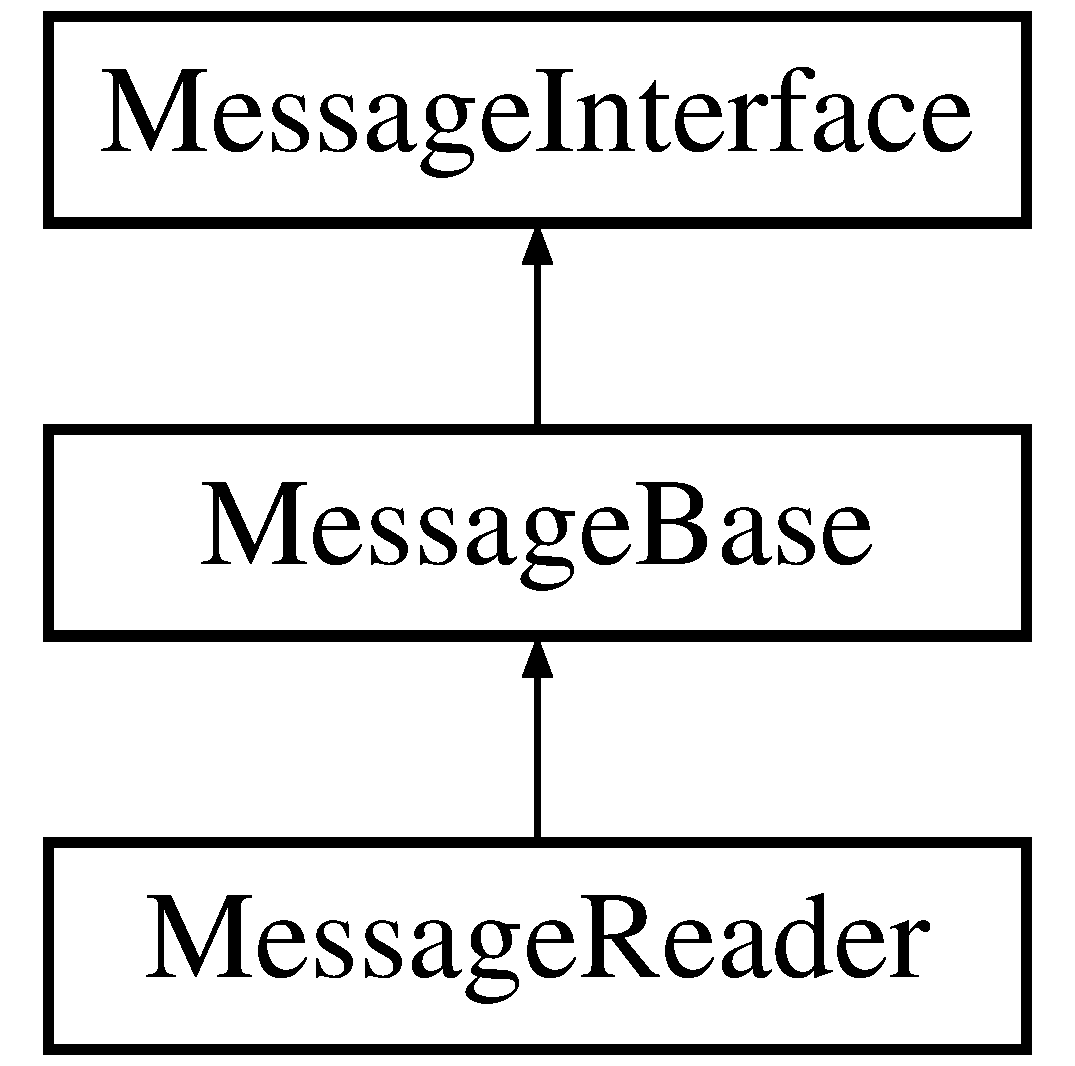
\includegraphics[height=3.000000cm]{class_message_base}
\end{center}
\end{figure}
\subsection*{Public Member Functions}
\begin{DoxyCompactItemize}
\item 
\mbox{\Hypertarget{class_message_base_ab750b4a7967fcd3e129d28a3ae1d4e86}\label{class_message_base_ab750b4a7967fcd3e129d28a3ae1d4e86}} 
void {\bfseries set\+Status\+Code} (int sc)
\item 
\mbox{\Hypertarget{class_message_base_a1340e12d07b6a0bbaff5221c3683c242}\label{class_message_base_a1340e12d07b6a0bbaff5221c3683c242}} 
void {\bfseries set\+Status} (std\+::string st)
\item 
\mbox{\Hypertarget{class_message_base_a030bbf498c20f1c2a2ce281ac69a1e61}\label{class_message_base_a030bbf498c20f1c2a2ce281ac69a1e61}} 
int {\bfseries status\+Code} ()
\item 
\mbox{\Hypertarget{class_message_base_a730462343be26eae0b3b56941c837c61}\label{class_message_base_a730462343be26eae0b3b56941c837c61}} 
std\+::string {\bfseries status} ()
\item 
\mbox{\Hypertarget{class_message_base_ac12869ed519facbe12e9fa9ee71e5d9b}\label{class_message_base_ac12869ed519facbe12e9fa9ee71e5d9b}} 
void {\bfseries set\+Method} (Http\+Method m)
\item 
\mbox{\Hypertarget{class_message_base_a917ec916c37524ff7a8c9b27c3d0bb98}\label{class_message_base_a917ec916c37524ff7a8c9b27c3d0bb98}} 
void {\bfseries set\+Method} (enum http\+\_\+method m)
\item 
\mbox{\Hypertarget{class_message_base_acfc91d36bdd4dd1b3828a03f5d427b54}\label{class_message_base_acfc91d36bdd4dd1b3828a03f5d427b54}} 
virtual void {\bfseries set\+Method} (std\+::string m\+\_\+str)
\item 
\mbox{\Hypertarget{class_message_base_a124e822086bf08600f83aa834ede9fce}\label{class_message_base_a124e822086bf08600f83aa834ede9fce}} 
std\+::string {\bfseries get\+Method\+As\+String} ()
\item 
\mbox{\Hypertarget{class_message_base_a21720424f7a3a95b0ee150cedf047789}\label{class_message_base_a21720424f7a3a95b0ee150cedf047789}} 
Http\+Method {\bfseries method} ()
\item 
\mbox{\Hypertarget{class_message_base_a23d29f983dd8ea011e21a974bdaa90b4}\label{class_message_base_a23d29f983dd8ea011e21a974bdaa90b4}} 
void {\bfseries set\+Uri} (std\+::string u)
\item 
\mbox{\Hypertarget{class_message_base_a71811fa2215104e4aaf504f0e51c377e}\label{class_message_base_a71811fa2215104e4aaf504f0e51c377e}} 
std\+::string {\bfseries uri} ()
\item 
\mbox{\Hypertarget{class_message_base_af56fe4e5b5a2857e7a2c95a1869c616b}\label{class_message_base_af56fe4e5b5a2857e7a2c95a1869c616b}} 
void {\bfseries set\+Http\+Vers\+Major} (int major)
\item 
\mbox{\Hypertarget{class_message_base_aefe31e700e9ed8af32229e24fddd8663}\label{class_message_base_aefe31e700e9ed8af32229e24fddd8663}} 
int {\bfseries http\+Vers\+Major} ()
\item 
\mbox{\Hypertarget{class_message_base_a3d0ed46204dbf8357cce7106906a139d}\label{class_message_base_a3d0ed46204dbf8357cce7106906a139d}} 
void {\bfseries set\+Http\+Vers\+Minor} (int minor)
\item 
\mbox{\Hypertarget{class_message_base_ae876fd4350b0413030a0c5385086bcc8}\label{class_message_base_ae876fd4350b0413030a0c5385086bcc8}} 
int {\bfseries http\+Vers\+Minor} ()
\item 
\mbox{\Hypertarget{class_message_base_aac4e29eb8556be7359c5d3259e09005e}\label{class_message_base_aac4e29eb8556be7359c5d3259e09005e}} 
void {\bfseries set\+Header} (std\+::string key, std\+::string value)
\item 
\mbox{\Hypertarget{class_message_base_a5d74045a5918ebb0b6a337e35d26993e}\label{class_message_base_a5d74045a5918ebb0b6a337e35d26993e}} 
bool {\bfseries has\+Header} (std\+::string key)
\item 
\mbox{\Hypertarget{class_message_base_a789c4f9ca6f44823daa8a1059f311590}\label{class_message_base_a789c4f9ca6f44823daa8a1059f311590}} 
std\+::string {\bfseries header} (std\+::string key)
\item 
\mbox{\Hypertarget{class_message_base_a98645e19e2b6722d581459bdd6c146dd}\label{class_message_base_a98645e19e2b6722d581459bdd6c146dd}} 
void {\bfseries remove\+Header} (std\+::string key)
\item 
\mbox{\Hypertarget{class_message_base_acf5d8a221c5c9a7d1a02c9c55798dda9}\label{class_message_base_acf5d8a221c5c9a7d1a02c9c55798dda9}} 
std\+::string {\bfseries get\+Header} (std\+::string key)
\item 
\mbox{\Hypertarget{class_message_base_a69869f3d0a88514d8254c583c707a3ec}\label{class_message_base_a69869f3d0a88514d8254c583c707a3ec}} 
std\+::map$<$ std\+::string, std\+::string $>$ \& {\bfseries get\+Headers} ()
\item 
\mbox{\Hypertarget{class_message_base_a2a6e0f2ebd74554871c2d1ceb13ad8a4}\label{class_message_base_a2a6e0f2ebd74554871c2d1ceb13ad8a4}} 
std\+::string {\bfseries str} ()
\item 
\mbox{\Hypertarget{class_message_base_a51e1e421b8938dc569ee5c6dea432ff7}\label{class_message_base_a51e1e421b8938dc569ee5c6dea432ff7}} 
void {\bfseries dump\+Headers} (std\+::ostream \&os)
\item 
\mbox{\Hypertarget{class_message_base_aa94bd648691d59a9848716bd9bd244ee}\label{class_message_base_aa94bd648691d59a9848716bd9bd244ee}} 
void {\bfseries set\+Trailer} (std\+::string key, std\+::string value)
\item 
\mbox{\Hypertarget{class_message_base_af8c76e1d4d2e6fcb2250ed7f32f3538b}\label{class_message_base_af8c76e1d4d2e6fcb2250ed7f32f3538b}} 
bool {\bfseries has\+Trailer} (std\+::string key)
\item 
\mbox{\Hypertarget{class_message_base_a8c80bb7c6504c19c78741fb92d97ef72}\label{class_message_base_a8c80bb7c6504c19c78741fb92d97ef72}} 
std\+::string {\bfseries trailer} (std\+::string key)
\item 
\mbox{\Hypertarget{class_message_base_acb033494a6cd68256589232ceea2ab09}\label{class_message_base_acb033494a6cd68256589232ceea2ab09}} 
void {\bfseries set\+Is\+Request} (bool flag)
\item 
\mbox{\Hypertarget{class_message_base_aed6742887d171862fd53d747d813491d}\label{class_message_base_aed6742887d171862fd53d747d813491d}} 
bool {\bfseries is\+Request} ()
\end{DoxyCompactItemize}
\subsection*{Protected Attributes}
\begin{DoxyCompactItemize}
\item 
\mbox{\Hypertarget{class_message_base_a647ba386ca25d115d68f9f3c86beebe8}\label{class_message_base_a647ba386ca25d115d68f9f3c86beebe8}} 
bool {\bfseries \+\_\+is\+\_\+request}
\item 
\mbox{\Hypertarget{class_message_base_a093ad4697fd2f03b394085fec74f2054}\label{class_message_base_a093ad4697fd2f03b394085fec74f2054}} 
enum http\+\_\+method {\bfseries \+\_\+method}
\item 
\mbox{\Hypertarget{class_message_base_a3c5d42001f69414a3bd627b0d1e5606e}\label{class_message_base_a3c5d42001f69414a3bd627b0d1e5606e}} 
std\+::string {\bfseries \+\_\+method\+Str}
\item 
\mbox{\Hypertarget{class_message_base_a7a830e02b75d652d4602b77ed8afd772}\label{class_message_base_a7a830e02b75d652d4602b77ed8afd772}} 
std\+::string {\bfseries \+\_\+uri}
\item 
\mbox{\Hypertarget{class_message_base_aa967b2e5fcf381851ca4b43aa42fdff6}\label{class_message_base_aa967b2e5fcf381851ca4b43aa42fdff6}} 
int {\bfseries \+\_\+status\+\_\+code}
\item 
\mbox{\Hypertarget{class_message_base_a9f697453b5e4c3d566bf929d7f1f67b3}\label{class_message_base_a9f697453b5e4c3d566bf929d7f1f67b3}} 
std\+::string {\bfseries \+\_\+status}
\item 
\mbox{\Hypertarget{class_message_base_aca700db308fc5b1708e08f40c9fbf2ec}\label{class_message_base_aca700db308fc5b1708e08f40c9fbf2ec}} 
int {\bfseries \+\_\+http\+\_\+major}
\item 
\mbox{\Hypertarget{class_message_base_a1507173e297eed53eb53c45f52d09054}\label{class_message_base_a1507173e297eed53eb53c45f52d09054}} 
int {\bfseries \+\_\+http\+\_\+minor}
\item 
\mbox{\Hypertarget{class_message_base_abc90275b70204447de92d1f20dd755c5}\label{class_message_base_abc90275b70204447de92d1f20dd755c5}} 
std\+::map$<$ std\+::string, std\+::string $>$ {\bfseries \+\_\+headers}
\item 
\mbox{\Hypertarget{class_message_base_a322ec7701cd03545071561600050aa5d}\label{class_message_base_a322ec7701cd03545071561600050aa5d}} 
std\+::map$<$ std\+::string, std\+::string $>$ {\bfseries \+\_\+trailers}
\end{DoxyCompactItemize}
\subsection*{Friends}
\begin{DoxyCompactItemize}
\item 
\mbox{\Hypertarget{class_message_base_acb21b1e7f1d029519af4fec437c4791b}\label{class_message_base_acb21b1e7f1d029519af4fec437c4791b}} 
std\+::string {\bfseries trace\+Message} (\hyperlink{class_message_base}{Message\+Base} \&msg)
\item 
\mbox{\Hypertarget{class_message_base_a2eab8867f8d6105bb286295df101bcb4}\label{class_message_base_a2eab8867f8d6105bb286295df101bcb4}} 
void {\bfseries serialize\+Headers} (\hyperlink{class_message_base}{Message\+Base} \&msg, \hyperlink{struct_m_buffer}{M\+Buffer} \&buf)
\end{DoxyCompactItemize}


The documentation for this class was generated from the following files\+:\begin{DoxyCompactItemize}
\item 
marvin/message/message.\+hpp\item 
marvin/message/message.\+cpp\end{DoxyCompactItemize}

\hypertarget{class_message_interface}{}\section{Message\+Interface Class Reference}
\label{class_message_interface}\index{Message\+Interface@{Message\+Interface}}
Inheritance diagram for Message\+Interface\+:\begin{figure}[H]
\begin{center}
\leavevmode
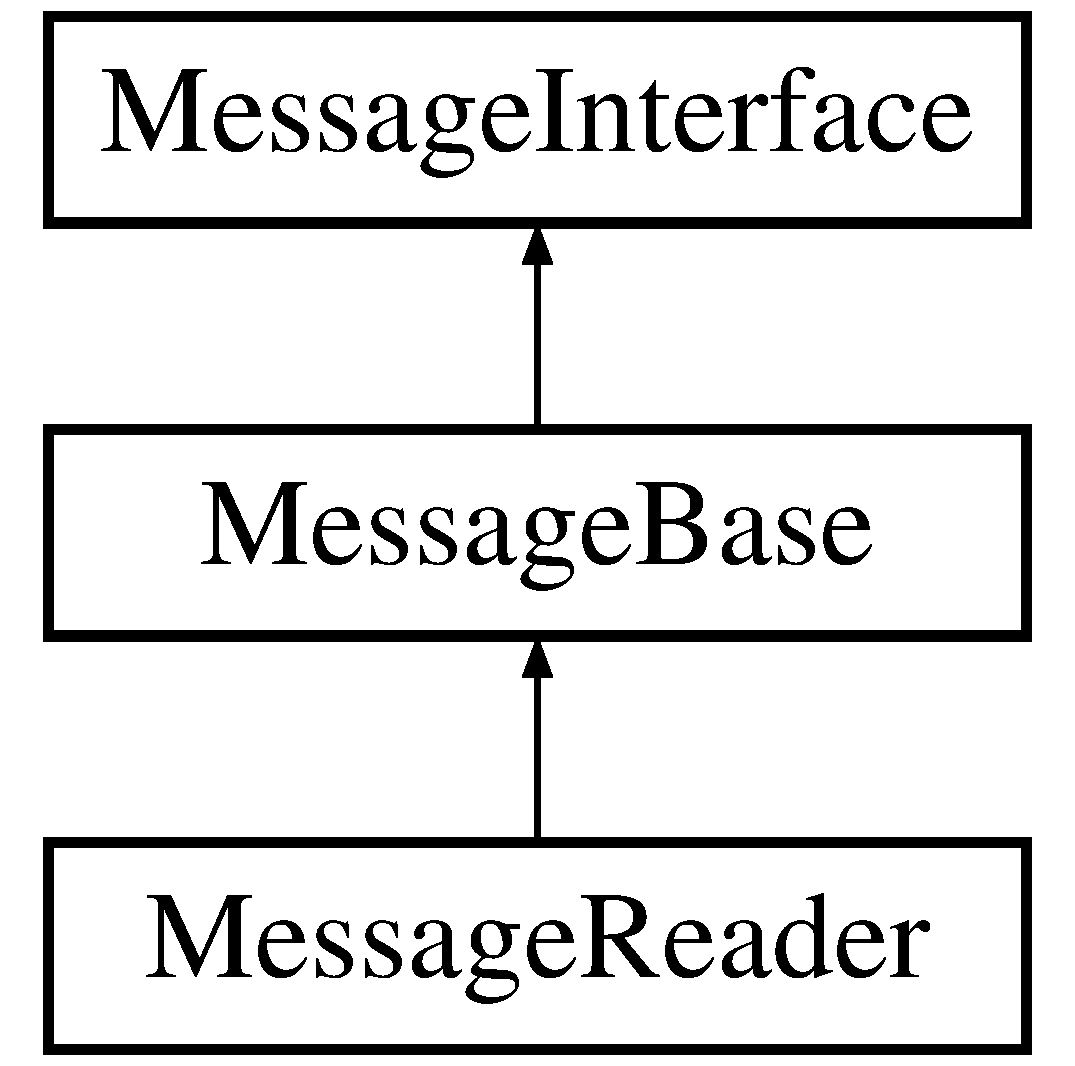
\includegraphics[height=3.000000cm]{class_message_interface}
\end{center}
\end{figure}
\subsection*{Public Member Functions}
\begin{DoxyCompactItemize}
\item 
\mbox{\Hypertarget{class_message_interface_aac5de86a7423b061331f4477cdb65e45}\label{class_message_interface_aac5de86a7423b061331f4477cdb65e45}} 
virtual void {\bfseries set\+Method} (Http\+Method m)=0
\item 
\mbox{\Hypertarget{class_message_interface_ac22f61b2a5fbc003b84b135549719101}\label{class_message_interface_ac22f61b2a5fbc003b84b135549719101}} 
virtual void {\bfseries set\+Method} (enum http\+\_\+method m)=0
\item 
\mbox{\Hypertarget{class_message_interface_a7c81d00f403337a3064881db3b9716e6}\label{class_message_interface_a7c81d00f403337a3064881db3b9716e6}} 
virtual void {\bfseries set\+Method} (std\+::string m\+\_\+str)=0
\item 
\mbox{\Hypertarget{class_message_interface_a06a16fde4d02ffdbf217ef010751bc66}\label{class_message_interface_a06a16fde4d02ffdbf217ef010751bc66}} 
virtual void {\bfseries set\+Uri} (std\+::string u)=0
\item 
\mbox{\Hypertarget{class_message_interface_a5f0e88434038d9af88e7a58ea31c9890}\label{class_message_interface_a5f0e88434038d9af88e7a58ea31c9890}} 
virtual std\+::string {\bfseries uri} ()=0
\item 
\mbox{\Hypertarget{class_message_interface_a378747430b897ae346c278c321c3a9c3}\label{class_message_interface_a378747430b897ae346c278c321c3a9c3}} 
virtual void {\bfseries set\+Status\+Code} (int sc)=0
\item 
\mbox{\Hypertarget{class_message_interface_ab3e8305b0795bfc372ad4767f46dce58}\label{class_message_interface_ab3e8305b0795bfc372ad4767f46dce58}} 
virtual int {\bfseries status\+Code} ()=0
\item 
\mbox{\Hypertarget{class_message_interface_accb5e2e87727e18ca3f244de4bf32f75}\label{class_message_interface_accb5e2e87727e18ca3f244de4bf32f75}} 
virtual void {\bfseries set\+Status} (std\+::string st)=0
\item 
\mbox{\Hypertarget{class_message_interface_a9497e1e1eb81cd527fb546a3dc5f2e30}\label{class_message_interface_a9497e1e1eb81cd527fb546a3dc5f2e30}} 
virtual std\+::string {\bfseries status} ()=0
\item 
\mbox{\Hypertarget{class_message_interface_a5926ad8da3b7b2613ea186e2e1e2cbf7}\label{class_message_interface_a5926ad8da3b7b2613ea186e2e1e2cbf7}} 
virtual void {\bfseries set\+Http\+Vers\+Major} (int major)=0
\item 
\mbox{\Hypertarget{class_message_interface_ad15146b7e0fc816acaa59e5a8c021b5e}\label{class_message_interface_ad15146b7e0fc816acaa59e5a8c021b5e}} 
virtual int {\bfseries http\+Vers\+Major} ()=0
\item 
\mbox{\Hypertarget{class_message_interface_a11180731a20ccf6ecffcf412520bd25b}\label{class_message_interface_a11180731a20ccf6ecffcf412520bd25b}} 
virtual void {\bfseries set\+Http\+Vers\+Minor} (int minor)=0
\item 
\mbox{\Hypertarget{class_message_interface_a85a71b2c6917d95ee0028271af7b2f84}\label{class_message_interface_a85a71b2c6917d95ee0028271af7b2f84}} 
virtual int {\bfseries http\+Vers\+Minor} ()=0
\item 
\mbox{\Hypertarget{class_message_interface_af5978ed2686bef1f14099cc13d268e59}\label{class_message_interface_af5978ed2686bef1f14099cc13d268e59}} 
virtual void {\bfseries set\+Header} (std\+::string key, std\+::string value)=0
\item 
\mbox{\Hypertarget{class_message_interface_a946396d0fbafb81ebce2a1e56f8f6251}\label{class_message_interface_a946396d0fbafb81ebce2a1e56f8f6251}} 
virtual std\+::string {\bfseries header} (std\+::string key)=0
\item 
\mbox{\Hypertarget{class_message_interface_a4633f3841d16d96b4885274c540c96c4}\label{class_message_interface_a4633f3841d16d96b4885274c540c96c4}} 
virtual void {\bfseries set\+Trailer} (std\+::string key, std\+::string value)=0
\item 
\mbox{\Hypertarget{class_message_interface_a18ad2751bb72126df4d7556482fc463c}\label{class_message_interface_a18ad2751bb72126df4d7556482fc463c}} 
virtual std\+::string {\bfseries trailer} (std\+::string key)=0
\item 
\mbox{\Hypertarget{class_message_interface_ac4f20cd49960e39c308aca5b525d2387}\label{class_message_interface_ac4f20cd49960e39c308aca5b525d2387}} 
virtual void {\bfseries set\+Is\+Request} (bool isrreq)=0
\item 
\mbox{\Hypertarget{class_message_interface_a370d5f87a452cfa7db19e61aa9585e95}\label{class_message_interface_a370d5f87a452cfa7db19e61aa9585e95}} 
virtual bool {\bfseries is\+Request} ()=0
\end{DoxyCompactItemize}


The documentation for this class was generated from the following file\+:\begin{DoxyCompactItemize}
\item 
marvin/message/message.\+hpp\end{DoxyCompactItemize}

\hypertarget{class_message_reader}{}\section{Message\+Reader Class Reference}
\label{class_message_reader}\index{Message\+Reader@{Message\+Reader}}
Inheritance diagram for Message\+Reader\+:\begin{figure}[H]
\begin{center}
\leavevmode
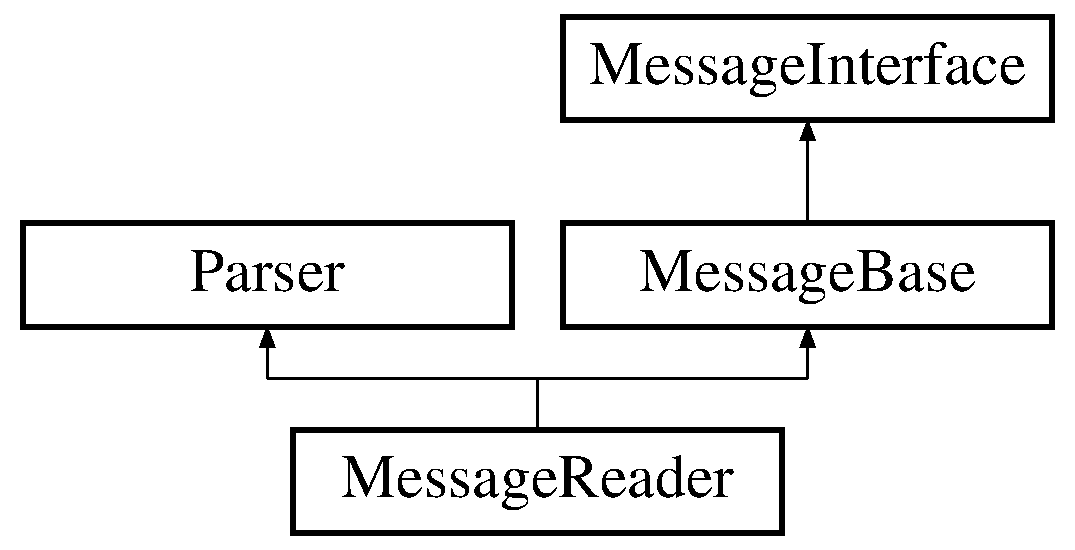
\includegraphics[height=3.000000cm]{class_message_reader}
\end{center}
\end{figure}
\subsection*{Public Member Functions}
\begin{DoxyCompactItemize}
\item 
\mbox{\Hypertarget{class_message_reader_a782500be6ba3210d3afc1cec4c68bd62}\label{class_message_reader_a782500be6ba3210d3afc1cec4c68bd62}} 
{\bfseries Message\+Reader} (boost\+::asio\+::io\+\_\+service \&io, Read\+Socket\+Interface\+S\+Ptr read\+Sock)
\item 
\hyperlink{class_message_reader_ab5a1832a8447dd11d8d57d8aed44d3a9}{$\sim$\+Message\+Reader} ()
\item 
void \hyperlink{class_message_reader_ab63fcdf1b67d82ce259d1e82775149a5}{read\+Headers} (std\+::function$<$ void(Marvin\+::\+Error\+Type err)$>$ cb)
\item 
void \hyperlink{class_message_reader_a811c0c6620e4bc7af99d5f519552846f}{read\+Body} (std\+::function$<$ void(Marvin\+::\+Error\+Type err, \hyperlink{class_buffer_chain}{Buffer\+Chain} chunk)$>$)
\item 
void \hyperlink{class_message_reader_a16e0cec435a29862c95cdccf61b3099b}{read\+Message} (std\+::function$<$ void(Marvin\+::\+Error\+Type err)$>$ cb)
\item 
\hyperlink{class_buffer_chain}{Buffer\+Chain} \hyperlink{class_message_reader_ac480fcf3e6f5b1bb89b467d372a4e435}{get\+\_\+body\+\_\+chain} ()
\item 
\hyperlink{class_buffer_chain}{Buffer\+Chain} \hyperlink{class_message_reader_a93a38a06b77aea962b76fab6f9ba77e2}{get\+\_\+raw\+\_\+body\+\_\+chain} ()
\end{DoxyCompactItemize}
\subsection*{Static Public Member Functions}
\begin{DoxyCompactItemize}
\item 
static void \hyperlink{class_message_reader_ab80bdac9cbb3d446a6d8b5e944ba3bfe}{config\+Set\+\_\+\+Header\+Buffer\+Size} (long bsize)
\item 
static void \hyperlink{class_message_reader_a83e245590821f3c60de01f698febac25}{config\+Set\+\_\+\+Body\+Buffer\+Size} (long bsize)
\end{DoxyCompactItemize}
\subsection*{Protected Member Functions}
\begin{DoxyCompactItemize}
\item 
void \hyperlink{class_message_reader_a9109576c1fd18d70e9187744164c390c}{read\+\_\+headers} (std\+::function$<$ void(Marvin\+::\+Error\+Type err)$>$ cb)
\item 
void \hyperlink{class_message_reader_a71a8b0ca7cc3aab28ee5fd9353f1b843}{read\+\_\+message} (std\+::function$<$ void(Marvin\+::\+Error\+Type err)$>$ cb)
\item 
void \hyperlink{class_message_reader_a73def02a6454f8c90df358790d798718}{\+\_\+read\+\_\+some\+\_\+headers} ()
\item 
void \hyperlink{class_message_reader_a545048a118c1d77940886544742dd9c0}{\+\_\+handle\+\_\+header\+\_\+read} (Marvin\+::\+Error\+Type er, std\+::size\+\_\+t bytes\+\_\+transfered)
\item 
\mbox{\Hypertarget{class_message_reader_a2f4c0d98a480e64f8d769c64f713b5c1}\label{class_message_reader_a2f4c0d98a480e64f8d769c64f713b5c1}} 
void {\bfseries read\+\_\+body} (std\+::function$<$ void(Marvin\+::\+Error\+Type err)$>$ cb)
\item 
void \hyperlink{class_message_reader_a5d38bae22274c77c8bf7b704aef2bccc}{\+\_\+read\+\_\+all\+\_\+body} ()
\item 
void \hyperlink{class_message_reader_acc54adf0f70b46dfcd73d017b1bb422c}{\+\_\+read\+\_\+some\+\_\+body} ()
\item 
void \hyperlink{class_message_reader_a366ff67eab28c15869657c436babf31e}{\+\_\+handle\+\_\+body\+\_\+read} (Marvin\+::\+Error\+Type er, std\+::size\+\_\+t bytes\+\_\+transfered)
\item 
void \hyperlink{class_message_reader_a10d3092b2b3200eaf9b69e49d36d1d69}{\+\_\+read\+\_\+body\+\_\+chunk} ()
\item 
void \hyperlink{class_message_reader_af174bd59d03d7e462f76d137b22863f2}{\+\_\+handle\+\_\+body\+\_\+chunk} (Marvin\+::\+Error\+Type er, std\+::size\+\_\+t bytes\+\_\+transfered)
\item 
void \hyperlink{class_message_reader_a4272b25b74e5b46f37754751da8689c5}{\+\_\+make\+\_\+new\+\_\+body\+\_\+buffer} ()
\item 
void \hyperlink{class_message_reader_a8df7f104650383e80e69a3d212b1e049}{post\+\_\+message\+\_\+cb} (Marvin\+::\+Error\+Type er)
\item 
void \hyperlink{class_message_reader_a82f75653a713d3b947ff3dee82a34d1f}{post\+\_\+body\+\_\+chunk\+\_\+cb} (Marvin\+::\+Error\+Type er, \hyperlink{class_buffer_chain}{Buffer\+Chain} chain)
\item 
bool \hyperlink{class_message_reader_a378b9c5f8136ac24865b5fac3c22694c}{parser\+\_\+ok} (int nparsed, \hyperlink{struct_m_buffer}{M\+Buffer} \&mb)
\item 
\hyperlink{class_message_interface}{Message\+Interface} $\ast$ \hyperlink{class_message_reader_a06ec9e561ff5cde8f4e1ffb0ff17cb1f}{current\+Message} ()
\item 
void \hyperlink{class_message_reader_a813dbc29f75b43f36ef3f770cc39c3e7}{On\+Headers\+Complete} (\hyperlink{class_message_interface}{Message\+Interface} $\ast$msg, void $\ast$body\+\_\+start\+\_\+ptr, std\+::size\+\_\+t remainder)
\item 
\mbox{\Hypertarget{class_message_reader_a5fb4fce3af6faf9ae8460d9d1bbede31}\label{class_message_reader_a5fb4fce3af6faf9ae8460d9d1bbede31}} 
void {\bfseries On\+Message\+Complete} (\hyperlink{class_message_interface}{Message\+Interface} $\ast$msg)
\item 
void \hyperlink{class_message_reader_a4f01917ce0c7c84159f81f797a7d13ec}{On\+Body\+Data} (void $\ast$buf, int len)
\item 
\mbox{\Hypertarget{class_message_reader_a3778ee11c827974e72d5c0e41abba654}\label{class_message_reader_a3778ee11c827974e72d5c0e41abba654}} 
void {\bfseries On\+Chunk\+Begin} (int chunk\+Length)
\item 
\mbox{\Hypertarget{class_message_reader_a193a61f82564385cc94520351c8c9608}\label{class_message_reader_a193a61f82564385cc94520351c8c9608}} 
void {\bfseries On\+Chunk\+Data} (void $\ast$buf, int len)
\item 
\mbox{\Hypertarget{class_message_reader_a3c64d95036ec88f48d87711512e3418c}\label{class_message_reader_a3c64d95036ec88f48d87711512e3418c}} 
void {\bfseries On\+Chunk\+End} ()
\end{DoxyCompactItemize}
\subsection*{Protected Attributes}
\begin{DoxyCompactItemize}
\item 
\mbox{\Hypertarget{class_message_reader_abb038487edc35f1ab52dda94905f12bf}\label{class_message_reader_abb038487edc35f1ab52dda94905f12bf}} 
bool {\bfseries \+\_\+reading\+\_\+full\+\_\+message}
\item 
\mbox{\Hypertarget{class_message_reader_a4f8033980198ae323904b1da61e04018}\label{class_message_reader_a4f8033980198ae323904b1da61e04018}} 
bool {\bfseries \+\_\+reading\+\_\+body}
\item 
\mbox{\Hypertarget{class_message_reader_a163ab2d455cc0309604eba34d98899fd}\label{class_message_reader_a163ab2d455cc0309604eba34d98899fd}} 
std\+::function$<$ void(Marvin\+::\+Error\+Type err)$>$ {\bfseries \+\_\+read\+\_\+message\+\_\+cb}
\item 
\mbox{\Hypertarget{class_message_reader_aafcafdb0a110e408fded627d6adb0437}\label{class_message_reader_aafcafdb0a110e408fded627d6adb0437}} 
std\+::function$<$ void(Marvin\+::\+Error\+Type err, \hyperlink{class_buffer_chain}{Buffer\+Chain} chunk)$>$ {\bfseries \+\_\+read\+\_\+body\+\_\+cb}
\item 
\mbox{\Hypertarget{class_message_reader_a2143042814a1309829b81b6e291c515a}\label{class_message_reader_a2143042814a1309829b81b6e291c515a}} 
int {\bfseries \+\_\+total\+\_\+bytes\+\_\+read}
\item 
\mbox{\Hypertarget{class_message_reader_a98f9607368a080b35b7d30659dfe69fa}\label{class_message_reader_a98f9607368a080b35b7d30659dfe69fa}} 
M\+Buffer\+S\+Ptr {\bfseries \+\_\+header\+\_\+buffer\+\_\+sptr}
\item 
\mbox{\Hypertarget{class_message_reader_a6b71ff33548f957df6c314802af2fcd9}\label{class_message_reader_a6b71ff33548f957df6c314802af2fcd9}} 
M\+Buffer\+S\+Ptr {\bfseries \+\_\+body\+\_\+buffer\+\_\+sptr}
\item 
\mbox{\Hypertarget{class_message_reader_a3411525f143e9e0ed3a072db10734f08}\label{class_message_reader_a3411525f143e9e0ed3a072db10734f08}} 
F\+Buffer\+Shared\+Ptr {\bfseries \+\_\+body\+\_\+fragments\+\_\+sptr}
\item 
\mbox{\Hypertarget{class_message_reader_ad12c7c3612b1bc785b36a3640ac1b859}\label{class_message_reader_ad12c7c3612b1bc785b36a3640ac1b859}} 
\hyperlink{class_buffer_chain}{Buffer\+Chain} {\bfseries \+\_\+raw\+\_\+body\+\_\+buffer\+\_\+chain}
\item 
\mbox{\Hypertarget{class_message_reader_a6e6d5c1c4ab54e7313c68742d0a8d4a7}\label{class_message_reader_a6e6d5c1c4ab54e7313c68742d0a8d4a7}} 
\hyperlink{class_buffer_chain}{Buffer\+Chain} {\bfseries \+\_\+body\+\_\+buffer\+\_\+chain}
\item 
\mbox{\Hypertarget{class_message_reader_aa678e062266320bfb530386be56b9c38}\label{class_message_reader_aa678e062266320bfb530386be56b9c38}} 
std\+::vector$<$ F\+Buffer\+Shared\+Ptr $>$ {\bfseries \+\_\+body\+\_\+fragments\+\_\+chain}
\item 
\mbox{\Hypertarget{class_message_reader_a8c59f3b342647abae8ad4693082fcc31}\label{class_message_reader_a8c59f3b342647abae8ad4693082fcc31}} 
Read\+Socket\+Interface\+S\+Ptr {\bfseries \+\_\+read\+Sock}
\item 
\mbox{\Hypertarget{class_message_reader_af95447697277c9ef993844b57c643591}\label{class_message_reader_af95447697277c9ef993844b57c643591}} 
boost\+::asio\+::io\+\_\+service \& {\bfseries \+\_\+io}
\item 
\mbox{\Hypertarget{class_message_reader_a12621c4803e1dff5d27e237ead132e08}\label{class_message_reader_a12621c4803e1dff5d27e237ead132e08}} 
std\+::size\+\_\+t {\bfseries \+\_\+body\+\_\+buffer\+\_\+size}
\item 
\mbox{\Hypertarget{class_message_reader_a6c2b39003410b82a8fb1fc8807c68bad}\label{class_message_reader_a6c2b39003410b82a8fb1fc8807c68bad}} 
std\+::size\+\_\+t {\bfseries \+\_\+header\+\_\+buffer\+\_\+size}
\item 
\mbox{\Hypertarget{class_message_reader_aa566ebe170a434558fa281037c7535d0}\label{class_message_reader_aa566ebe170a434558fa281037c7535d0}} 
bool {\bfseries \+\_\+read\+Body\+Started}
\item 
\mbox{\Hypertarget{class_message_reader_a39dc9d4c6c5b16c73a55f1f89ed22b16}\label{class_message_reader_a39dc9d4c6c5b16c73a55f1f89ed22b16}} 
\hyperlink{struct_m_buffer}{M\+Buffer} $\ast$ {\bfseries \+\_\+body\+M\+Buffer\+Ptr}
\item 
\mbox{\Hypertarget{class_message_reader_a5e48aeb6d413b756ae8a6a84d830e25d}\label{class_message_reader_a5e48aeb6d413b756ae8a6a84d830e25d}} 
\hyperlink{class_f_buffer}{F\+Buffer} $\ast$ {\bfseries \+\_\+body\+F\+Buffer\+Ptr}
\item 
\mbox{\Hypertarget{class_message_reader_a2ce5dc510e084fa7dc3cc94d5d699277}\label{class_message_reader_a2ce5dc510e084fa7dc3cc94d5d699277}} 
\hyperlink{struct_m_buffer}{M\+Buffer} $\ast$ {\bfseries \+\_\+read\+Buffer}
\item 
\mbox{\Hypertarget{class_message_reader_a47692db94154e8ba7efda892403df476}\label{class_message_reader_a47692db94154e8ba7efda892403df476}} 
std\+::string \hyperlink{class_message_reader_a47692db94154e8ba7efda892403df476}{body}
\begin{DoxyCompactList}\small\item\em used for full message read -\/ body collection \end{DoxyCompactList}\item 
\mbox{\Hypertarget{class_message_reader_a37fd89ff6258ad48b915e625558e1bbc}\label{class_message_reader_a37fd89ff6258ad48b915e625558e1bbc}} 
std\+::ostringstream {\bfseries body\+Stream}
\item 
\mbox{\Hypertarget{class_message_reader_aeb3d223497993154acca83dc6ec9eaa2}\label{class_message_reader_aeb3d223497993154acca83dc6ec9eaa2}} 
Read\+Body\+Data\+Callback\+Type {\bfseries \+\_\+body\+Callback}
\item 
\mbox{\Hypertarget{class_message_reader_a146a65cba204e9aa401484adc230be32}\label{class_message_reader_a146a65cba204e9aa401484adc230be32}} 
Read\+Headers\+Callback\+Type {\bfseries \+\_\+response\+Cb}
\item 
\mbox{\Hypertarget{class_message_reader_a7ad01d613200dec83fb0d0a6a71edb77}\label{class_message_reader_a7ad01d613200dec83fb0d0a6a71edb77}} 
Read\+Message\+Callback\+Type {\bfseries \+\_\+message\+Cb}
\end{DoxyCompactItemize}
\subsection*{Static Protected Attributes}
\begin{DoxyCompactItemize}
\item 
\mbox{\Hypertarget{class_message_reader_a99feadce4d7a038210448aec87a44d90}\label{class_message_reader_a99feadce4d7a038210448aec87a44d90}} 
static std\+::size\+\_\+t {\bfseries \+\_\+\+\_\+header\+Buffer\+Size} = 10000
\item 
\mbox{\Hypertarget{class_message_reader_a7881cc09f4b6f7e45aa21c5a613d7d2c}\label{class_message_reader_a7881cc09f4b6f7e45aa21c5a613d7d2c}} 
static std\+::size\+\_\+t {\bfseries \+\_\+\+\_\+body\+Buffer\+Size} = 20000
\end{DoxyCompactItemize}
\subsection*{Friends}
\begin{DoxyCompactItemize}
\item 
\mbox{\Hypertarget{class_message_reader_a15c731cddafc776dccca9000ad701b43}\label{class_message_reader_a15c731cddafc776dccca9000ad701b43}} 
std\+::string {\bfseries trace\+Reader} (\hyperlink{class_message_reader}{Message\+Reader} \&rdr)
\end{DoxyCompactItemize}


\subsection{Constructor \& Destructor Documentation}
\mbox{\Hypertarget{class_message_reader_ab5a1832a8447dd11d8d57d8aed44d3a9}\label{class_message_reader_ab5a1832a8447dd11d8d57d8aed44d3a9}} 
\index{Message\+Reader@{Message\+Reader}!````~Message\+Reader@{$\sim$\+Message\+Reader}}
\index{````~Message\+Reader@{$\sim$\+Message\+Reader}!Message\+Reader@{Message\+Reader}}
\subsubsection{\texorpdfstring{$\sim$\+Message\+Reader()}{~MessageReader()}}
{\footnotesize\ttfamily Message\+Reader\+::$\sim$\+Message\+Reader (\begin{DoxyParamCaption}{ }\end{DoxyParamCaption})}

Destructor -\/ nothing to do. All pointers held by an instance are smart pointers. 

\subsection{Member Function Documentation}
\mbox{\Hypertarget{class_message_reader_af174bd59d03d7e462f76d137b22863f2}\label{class_message_reader_af174bd59d03d7e462f76d137b22863f2}} 
\index{Message\+Reader@{Message\+Reader}!\+\_\+handle\+\_\+body\+\_\+chunk@{\+\_\+handle\+\_\+body\+\_\+chunk}}
\index{\+\_\+handle\+\_\+body\+\_\+chunk@{\+\_\+handle\+\_\+body\+\_\+chunk}!Message\+Reader@{Message\+Reader}}
\subsubsection{\texorpdfstring{\+\_\+handle\+\_\+body\+\_\+chunk()}{\_handle\_body\_chunk()}}
{\footnotesize\ttfamily void Message\+Reader\+::\+\_\+handle\+\_\+body\+\_\+chunk (\begin{DoxyParamCaption}\item[{Marvin\+::\+Error\+Type}]{er,  }\item[{std\+::size\+\_\+t}]{bytes\+\_\+transfered }\end{DoxyParamCaption})\hspace{0.3cm}{\ttfamily [protected]}}

Completion handler for reading a single chunk of body data. an io error with bytes\+\_\+transfered == 0 is probably E\+OF -\/ let the parser handle it otherwise (err \&\& (bytes\+\_\+transfered $>$ 0)) return with error\mbox{\Hypertarget{class_message_reader_a366ff67eab28c15869657c436babf31e}\label{class_message_reader_a366ff67eab28c15869657c436babf31e}} 
\index{Message\+Reader@{Message\+Reader}!\+\_\+handle\+\_\+body\+\_\+read@{\+\_\+handle\+\_\+body\+\_\+read}}
\index{\+\_\+handle\+\_\+body\+\_\+read@{\+\_\+handle\+\_\+body\+\_\+read}!Message\+Reader@{Message\+Reader}}
\subsubsection{\texorpdfstring{\+\_\+handle\+\_\+body\+\_\+read()}{\_handle\_body\_read()}}
{\footnotesize\ttfamily void Message\+Reader\+::\+\_\+handle\+\_\+body\+\_\+read (\begin{DoxyParamCaption}\item[{Marvin\+::\+Error\+Type}]{er,  }\item[{std\+::size\+\_\+t}]{bytes\+\_\+transfered }\end{DoxyParamCaption})\hspace{0.3cm}{\ttfamily [protected]}}

Step two of the async loop that reads all body data. This is the async completion handler. an io error with bytes\+\_\+transfered == 0 is probably E\+OF -\/ let the parser handle it otherwise (err \&\& (bytes\+\_\+transfered $>$ 0)) return with error\mbox{\Hypertarget{class_message_reader_a545048a118c1d77940886544742dd9c0}\label{class_message_reader_a545048a118c1d77940886544742dd9c0}} 
\index{Message\+Reader@{Message\+Reader}!\+\_\+handle\+\_\+header\+\_\+read@{\+\_\+handle\+\_\+header\+\_\+read}}
\index{\+\_\+handle\+\_\+header\+\_\+read@{\+\_\+handle\+\_\+header\+\_\+read}!Message\+Reader@{Message\+Reader}}
\subsubsection{\texorpdfstring{\+\_\+handle\+\_\+header\+\_\+read()}{\_handle\_header\_read()}}
{\footnotesize\ttfamily void Message\+Reader\+::\+\_\+handle\+\_\+header\+\_\+read (\begin{DoxyParamCaption}\item[{Marvin\+::\+Error\+Type}]{er,  }\item[{std\+::size\+\_\+t}]{bytes\+\_\+transfered }\end{DoxyParamCaption})\hspace{0.3cm}{\ttfamily [protected]}}

Step two in an async loop to read all headers. This is the async completion handler for reading headers Error processing here is a bit tricky
\begin{DoxyItemize}
\item if we are in the middle of processing a messages and we get an io error with bytes\+\_\+transfered == 0, it is probably the other end sending an E\+OF to signal E\+OM so let the parser handle it
\item if this is the first result for a new message and bytes\+\_\+transfered ==0 this is probably the other end signalling socket closed and a new message is not being sent. In this case we dont want the parse to see the E\+OF as it wont treat it as an error and will keep trying to read. want to pass it to the callback as E\+OF
\item otherwise (err \&\& (bytes\+\_\+transfered $>$ 0)) return with error. For testing purposes we have to differentiate between ending a message with E\+OF and signalling connection closed with E\+OF
\end{DoxyItemize}\mbox{\Hypertarget{class_message_reader_a4272b25b74e5b46f37754751da8689c5}\label{class_message_reader_a4272b25b74e5b46f37754751da8689c5}} 
\index{Message\+Reader@{Message\+Reader}!\+\_\+make\+\_\+new\+\_\+body\+\_\+buffer@{\+\_\+make\+\_\+new\+\_\+body\+\_\+buffer}}
\index{\+\_\+make\+\_\+new\+\_\+body\+\_\+buffer@{\+\_\+make\+\_\+new\+\_\+body\+\_\+buffer}!Message\+Reader@{Message\+Reader}}
\subsubsection{\texorpdfstring{\+\_\+make\+\_\+new\+\_\+body\+\_\+buffer()}{\_make\_new\_body\_buffer()}}
{\footnotesize\ttfamily void Message\+Reader\+::\+\_\+make\+\_\+new\+\_\+body\+\_\+buffer (\begin{DoxyParamCaption}{ }\end{DoxyParamCaption})\hspace{0.3cm}{\ttfamily [protected]}}

Creates a shared pointer to a single new buffer for reading body data. \mbox{\Hypertarget{class_message_reader_a5d38bae22274c77c8bf7b704aef2bccc}\label{class_message_reader_a5d38bae22274c77c8bf7b704aef2bccc}} 
\index{Message\+Reader@{Message\+Reader}!\+\_\+read\+\_\+all\+\_\+body@{\+\_\+read\+\_\+all\+\_\+body}}
\index{\+\_\+read\+\_\+all\+\_\+body@{\+\_\+read\+\_\+all\+\_\+body}!Message\+Reader@{Message\+Reader}}
\subsubsection{\texorpdfstring{\+\_\+read\+\_\+all\+\_\+body()}{\_read\_all\_body()}}
{\footnotesize\ttfamily void Message\+Reader\+::\+\_\+read\+\_\+all\+\_\+body (\begin{DoxyParamCaption}{ }\end{DoxyParamCaption})\hspace{0.3cm}{\ttfamily [protected]}}

Kicks off the process of reading all body data. \mbox{\Hypertarget{class_message_reader_a10d3092b2b3200eaf9b69e49d36d1d69}\label{class_message_reader_a10d3092b2b3200eaf9b69e49d36d1d69}} 
\index{Message\+Reader@{Message\+Reader}!\+\_\+read\+\_\+body\+\_\+chunk@{\+\_\+read\+\_\+body\+\_\+chunk}}
\index{\+\_\+read\+\_\+body\+\_\+chunk@{\+\_\+read\+\_\+body\+\_\+chunk}!Message\+Reader@{Message\+Reader}}
\subsubsection{\texorpdfstring{\+\_\+read\+\_\+body\+\_\+chunk()}{\_read\_body\_chunk()}}
{\footnotesize\ttfamily void Message\+Reader\+::\+\_\+read\+\_\+body\+\_\+chunk (\begin{DoxyParamCaption}{ }\end{DoxyParamCaption})\hspace{0.3cm}{\ttfamily [protected]}}

Called by interface method \hyperlink{class_message_reader_a811c0c6620e4bc7af99d5f519552846f}{read\+Body()} Initiates the process of reading O\+NE chunk of body data. Sets up a read and completion handler. No looping for this \mbox{\Hypertarget{class_message_reader_acc54adf0f70b46dfcd73d017b1bb422c}\label{class_message_reader_acc54adf0f70b46dfcd73d017b1bb422c}} 
\index{Message\+Reader@{Message\+Reader}!\+\_\+read\+\_\+some\+\_\+body@{\+\_\+read\+\_\+some\+\_\+body}}
\index{\+\_\+read\+\_\+some\+\_\+body@{\+\_\+read\+\_\+some\+\_\+body}!Message\+Reader@{Message\+Reader}}
\subsubsection{\texorpdfstring{\+\_\+read\+\_\+some\+\_\+body()}{\_read\_some\_body()}}
{\footnotesize\ttfamily void Message\+Reader\+::\+\_\+read\+\_\+some\+\_\+body (\begin{DoxyParamCaption}{ }\end{DoxyParamCaption})\hspace{0.3cm}{\ttfamily [protected]}}

First part of an async loop that reads all body data. This method sets up and initiates an async read \mbox{\Hypertarget{class_message_reader_a73def02a6454f8c90df358790d798718}\label{class_message_reader_a73def02a6454f8c90df358790d798718}} 
\index{Message\+Reader@{Message\+Reader}!\+\_\+read\+\_\+some\+\_\+headers@{\+\_\+read\+\_\+some\+\_\+headers}}
\index{\+\_\+read\+\_\+some\+\_\+headers@{\+\_\+read\+\_\+some\+\_\+headers}!Message\+Reader@{Message\+Reader}}
\subsubsection{\texorpdfstring{\+\_\+read\+\_\+some\+\_\+headers()}{\_read\_some\_headers()}}
{\footnotesize\ttfamily void Message\+Reader\+::\+\_\+read\+\_\+some\+\_\+headers (\begin{DoxyParamCaption}{ }\end{DoxyParamCaption})\hspace{0.3cm}{\ttfamily [protected]}}

The first step in a two part async loop that reads all headers (until headers\+Complete) This function sets up and initiates a read. \mbox{\Hypertarget{class_message_reader_a83e245590821f3c60de01f698febac25}\label{class_message_reader_a83e245590821f3c60de01f698febac25}} 
\index{Message\+Reader@{Message\+Reader}!config\+Set\+\_\+\+Body\+Buffer\+Size@{config\+Set\+\_\+\+Body\+Buffer\+Size}}
\index{config\+Set\+\_\+\+Body\+Buffer\+Size@{config\+Set\+\_\+\+Body\+Buffer\+Size}!Message\+Reader@{Message\+Reader}}
\subsubsection{\texorpdfstring{config\+Set\+\_\+\+Body\+Buffer\+Size()}{configSet\_BodyBufferSize()}}
{\footnotesize\ttfamily void Message\+Reader\+::config\+Set\+\_\+\+Body\+Buffer\+Size (\begin{DoxyParamCaption}\item[{long}]{bsize }\end{DoxyParamCaption})\hspace{0.3cm}{\ttfamily [static]}}

Called at program startup to override the default value for the body buffer \mbox{\Hypertarget{class_message_reader_ab80bdac9cbb3d446a6d8b5e944ba3bfe}\label{class_message_reader_ab80bdac9cbb3d446a6d8b5e944ba3bfe}} 
\index{Message\+Reader@{Message\+Reader}!config\+Set\+\_\+\+Header\+Buffer\+Size@{config\+Set\+\_\+\+Header\+Buffer\+Size}}
\index{config\+Set\+\_\+\+Header\+Buffer\+Size@{config\+Set\+\_\+\+Header\+Buffer\+Size}!Message\+Reader@{Message\+Reader}}
\subsubsection{\texorpdfstring{config\+Set\+\_\+\+Header\+Buffer\+Size()}{configSet\_HeaderBufferSize()}}
{\footnotesize\ttfamily void Message\+Reader\+::config\+Set\+\_\+\+Header\+Buffer\+Size (\begin{DoxyParamCaption}\item[{long}]{bsize }\end{DoxyParamCaption})\hspace{0.3cm}{\ttfamily [static]}}

Called at program startup to override the default value for the haeder buffer \mbox{\Hypertarget{class_message_reader_a06ec9e561ff5cde8f4e1ffb0ff17cb1f}\label{class_message_reader_a06ec9e561ff5cde8f4e1ffb0ff17cb1f}} 
\index{Message\+Reader@{Message\+Reader}!current\+Message@{current\+Message}}
\index{current\+Message@{current\+Message}!Message\+Reader@{Message\+Reader}}
\subsubsection{\texorpdfstring{current\+Message()}{currentMessage()}}
{\footnotesize\ttfamily \hyperlink{class_message_interface}{Message\+Interface} $\ast$ Message\+Reader\+::current\+Message (\begin{DoxyParamCaption}{ }\end{DoxyParamCaption})\hspace{0.3cm}{\ttfamily [protected]}, {\ttfamily [virtual]}}

These methods are overridesa for virtual methods in Paser 

Implements \hyperlink{class_parser_a7b3c3ac1cf86a5f9fdda1ecf06dcd4dc}{Parser}.

\mbox{\Hypertarget{class_message_reader_ac480fcf3e6f5b1bb89b467d372a4e435}\label{class_message_reader_ac480fcf3e6f5b1bb89b467d372a4e435}} 
\index{Message\+Reader@{Message\+Reader}!get\+\_\+body\+\_\+chain@{get\+\_\+body\+\_\+chain}}
\index{get\+\_\+body\+\_\+chain@{get\+\_\+body\+\_\+chain}!Message\+Reader@{Message\+Reader}}
\subsubsection{\texorpdfstring{get\+\_\+body\+\_\+chain()}{get\_body\_chain()}}
{\footnotesize\ttfamily \hyperlink{class_buffer_chain}{Buffer\+Chain} Message\+Reader\+::get\+\_\+body\+\_\+chain (\begin{DoxyParamCaption}{ }\end{DoxyParamCaption})}

Gets the message body as a std\+::string !!! need to do better

accesses the \hyperlink{class_buffer_chain}{Buffer\+Chain} containing the de-\/chunked body data \mbox{\Hypertarget{class_message_reader_a93a38a06b77aea962b76fab6f9ba77e2}\label{class_message_reader_a93a38a06b77aea962b76fab6f9ba77e2}} 
\index{Message\+Reader@{Message\+Reader}!get\+\_\+raw\+\_\+body\+\_\+chain@{get\+\_\+raw\+\_\+body\+\_\+chain}}
\index{get\+\_\+raw\+\_\+body\+\_\+chain@{get\+\_\+raw\+\_\+body\+\_\+chain}!Message\+Reader@{Message\+Reader}}
\subsubsection{\texorpdfstring{get\+\_\+raw\+\_\+body\+\_\+chain()}{get\_raw\_body\_chain()}}
{\footnotesize\ttfamily \hyperlink{class_buffer_chain}{Buffer\+Chain} Message\+Reader\+::get\+\_\+raw\+\_\+body\+\_\+chain (\begin{DoxyParamCaption}{ }\end{DoxyParamCaption})}

accesses the \hyperlink{class_buffer_chain}{Buffer\+Chain} containing the raw (not de-\/chunked) body data \mbox{\Hypertarget{class_message_reader_a4f01917ce0c7c84159f81f797a7d13ec}\label{class_message_reader_a4f01917ce0c7c84159f81f797a7d13ec}} 
\index{Message\+Reader@{Message\+Reader}!On\+Body\+Data@{On\+Body\+Data}}
\index{On\+Body\+Data@{On\+Body\+Data}!Message\+Reader@{Message\+Reader}}
\subsubsection{\texorpdfstring{On\+Body\+Data()}{OnBodyData()}}
{\footnotesize\ttfamily void Message\+Reader\+::\+On\+Body\+Data (\begin{DoxyParamCaption}\item[{void $\ast$}]{buf,  }\item[{int}]{len }\end{DoxyParamCaption})\hspace{0.3cm}{\ttfamily [protected]}, {\ttfamily [virtual]}}

Overrides a \hyperlink{class_parser}{Parser} virtual method. Called whenever the http\+\_\+parser sees a piece of body data

This function is the only place where each piece of body data whether chunked or not is seen. Hence the only place to catch body data reliably. 

Reimplemented from \hyperlink{class_parser}{Parser}.

\mbox{\Hypertarget{class_message_reader_a813dbc29f75b43f36ef3f770cc39c3e7}\label{class_message_reader_a813dbc29f75b43f36ef3f770cc39c3e7}} 
\index{Message\+Reader@{Message\+Reader}!On\+Headers\+Complete@{On\+Headers\+Complete}}
\index{On\+Headers\+Complete@{On\+Headers\+Complete}!Message\+Reader@{Message\+Reader}}
\subsubsection{\texorpdfstring{On\+Headers\+Complete()}{OnHeadersComplete()}}
{\footnotesize\ttfamily void Message\+Reader\+::\+On\+Headers\+Complete (\begin{DoxyParamCaption}\item[{\hyperlink{class_message_interface}{Message\+Interface} $\ast$}]{msg,  }\item[{void $\ast$}]{body\+\_\+start\+\_\+ptr,  }\item[{std\+::size\+\_\+t}]{remainder }\end{DoxyParamCaption})\hspace{0.3cm}{\ttfamily [protected]}, {\ttfamily [virtual]}}

\begin{DoxyNote}{Note}
W\+A\+R\+N\+I\+NG -\/ http\+\_\+parser has been modified. The interface to this function and that of headers\+\_\+complete\+\_\+cb required by http\+\_\+parser have been modified (and that required a few lines of change in http\+\_\+parser) to provide the address in the current buffer of the first byte of body data in that same buffer, together with the length of the unparsed buffer at the time of headers complete. This is the only way of capturing a chunk header that happened to be in the same buffer as the last of the header data. If remander is N\+OT zero then some body data (maybe only chunk header) was in the buffer with the last of the header data. 
\end{DoxyNote}


Reimplemented from \hyperlink{class_parser}{Parser}.

\mbox{\Hypertarget{class_message_reader_a378b9c5f8136ac24865b5fac3c22694c}\label{class_message_reader_a378b9c5f8136ac24865b5fac3c22694c}} 
\index{Message\+Reader@{Message\+Reader}!parser\+\_\+ok@{parser\+\_\+ok}}
\index{parser\+\_\+ok@{parser\+\_\+ok}!Message\+Reader@{Message\+Reader}}
\subsubsection{\texorpdfstring{parser\+\_\+ok()}{parser\_ok()}}
{\footnotesize\ttfamily bool Message\+Reader\+::parser\+\_\+ok (\begin{DoxyParamCaption}\item[{int}]{nparsed,  }\item[{\hyperlink{struct_m_buffer}{M\+Buffer} \&}]{mb }\end{DoxyParamCaption})\hspace{0.3cm}{\ttfamily [protected]}}

if parser status is OK or if (http\+\_\+parser-\/$>$errno == H\+P\+E\+\_\+\+P\+A\+U\+S\+ED \&\& \hyperlink{class_parser_ad9d6c98af922409a78ff65083b1983e3}{is\+Finished\+Message()}) then we are OK with this message -\/ parsing is paused on E\+OM otherwise parser errors should be returned as errors\mbox{\Hypertarget{class_message_reader_a82f75653a713d3b947ff3dee82a34d1f}\label{class_message_reader_a82f75653a713d3b947ff3dee82a34d1f}} 
\index{Message\+Reader@{Message\+Reader}!post\+\_\+body\+\_\+chunk\+\_\+cb@{post\+\_\+body\+\_\+chunk\+\_\+cb}}
\index{post\+\_\+body\+\_\+chunk\+\_\+cb@{post\+\_\+body\+\_\+chunk\+\_\+cb}!Message\+Reader@{Message\+Reader}}
\subsubsection{\texorpdfstring{post\+\_\+body\+\_\+chunk\+\_\+cb()}{post\_body\_chunk\_cb()}}
{\footnotesize\ttfamily void Message\+Reader\+::post\+\_\+body\+\_\+chunk\+\_\+cb (\begin{DoxyParamCaption}\item[{Marvin\+::\+Error\+Type}]{er,  }\item[{\hyperlink{class_buffer_chain}{Buffer\+Chain}}]{chain }\end{DoxyParamCaption})\hspace{0.3cm}{\ttfamily [protected]}}

Schedules the execution of the \+\_\+read\+\_\+message\+\_\+cb in the future on this instances io\+\_\+service or runloop. \+\_\+read\+\_\+body\+\_\+cb is a property that stores the address of the callback provided to \hyperlink{class_message_reader_a811c0c6620e4bc7af99d5f519552846f}{read\+Body()}; \mbox{\Hypertarget{class_message_reader_a8df7f104650383e80e69a3d212b1e049}\label{class_message_reader_a8df7f104650383e80e69a3d212b1e049}} 
\index{Message\+Reader@{Message\+Reader}!post\+\_\+message\+\_\+cb@{post\+\_\+message\+\_\+cb}}
\index{post\+\_\+message\+\_\+cb@{post\+\_\+message\+\_\+cb}!Message\+Reader@{Message\+Reader}}
\subsubsection{\texorpdfstring{post\+\_\+message\+\_\+cb()}{post\_message\_cb()}}
{\footnotesize\ttfamily void Message\+Reader\+::post\+\_\+message\+\_\+cb (\begin{DoxyParamCaption}\item[{Marvin\+::\+Error\+Type}]{er }\end{DoxyParamCaption})\hspace{0.3cm}{\ttfamily [protected]}}

Schedules the execution of the \+\_\+read\+\_\+message\+\_\+cb in the future on this instances io\+\_\+service or runloop. \+\_\+read\+\_\+message\+\_\+cb is a property that stores the address of the callback provided to \hyperlink{class_message_reader_a16e0cec435a29862c95cdccf61b3099b}{read\+Message()} and \hyperlink{class_message_reader_ab63fcdf1b67d82ce259d1e82775149a5}{read\+Headers()} interface methods. \mbox{\Hypertarget{class_message_reader_a9109576c1fd18d70e9187744164c390c}\label{class_message_reader_a9109576c1fd18d70e9187744164c390c}} 
\index{Message\+Reader@{Message\+Reader}!read\+\_\+headers@{read\+\_\+headers}}
\index{read\+\_\+headers@{read\+\_\+headers}!Message\+Reader@{Message\+Reader}}
\subsubsection{\texorpdfstring{read\+\_\+headers()}{read\_headers()}}
{\footnotesize\ttfamily void Message\+Reader\+::read\+\_\+headers (\begin{DoxyParamCaption}\item[{std\+::function$<$ void(Marvin\+::\+Error\+Type err)$>$}]{cb }\end{DoxyParamCaption})\hspace{0.3cm}{\ttfamily [protected]}}

called by interface method read\+Headers to start the reading of headers without reading body data. Note the setting of \+\_\+reading\+\_\+full\+\_\+message = false \mbox{\Hypertarget{class_message_reader_a71a8b0ca7cc3aab28ee5fd9353f1b843}\label{class_message_reader_a71a8b0ca7cc3aab28ee5fd9353f1b843}} 
\index{Message\+Reader@{Message\+Reader}!read\+\_\+message@{read\+\_\+message}}
\index{read\+\_\+message@{read\+\_\+message}!Message\+Reader@{Message\+Reader}}
\subsubsection{\texorpdfstring{read\+\_\+message()}{read\_message()}}
{\footnotesize\ttfamily void Message\+Reader\+::read\+\_\+message (\begin{DoxyParamCaption}\item[{std\+::function$<$ void(Marvin\+::\+Error\+Type err)$>$}]{cb }\end{DoxyParamCaption})\hspace{0.3cm}{\ttfamily [protected]}}

Called interface method read\+Message to start the reading of headers and followed by the reading of all body data. Note the setting of \+\_\+reading\+\_\+full\+\_\+message = true \mbox{\Hypertarget{class_message_reader_a811c0c6620e4bc7af99d5f519552846f}\label{class_message_reader_a811c0c6620e4bc7af99d5f519552846f}} 
\index{Message\+Reader@{Message\+Reader}!read\+Body@{read\+Body}}
\index{read\+Body@{read\+Body}!Message\+Reader@{Message\+Reader}}
\subsubsection{\texorpdfstring{read\+Body()}{readBody()}}
{\footnotesize\ttfamily void Message\+Reader\+::read\+Body (\begin{DoxyParamCaption}\item[{std\+::function$<$ void(Marvin\+::\+Error\+Type err, \hyperlink{class_buffer_chain}{Buffer\+Chain} chunk)$>$}]{cb }\end{DoxyParamCaption})}

This methods read the body data. Should be called multiple times until the end of message body is signalled by the returned error code being equal to Marvin\+::make\+\_\+error\+\_\+eob() or or Marvin\+::make\+\_\+error\+\_\+eom()

The callback to read\+Body receives an error code and an instance (by value) of a \hyperlink{class_buffer_chain}{Buffer\+Chain} This is because the body data returned in that buffer is \char`\"{}de-\/chunked\char`\"{} and the buffer M\+AY contain multiple chunk bodies. It was done this way to prevent copying the body data to eliminate the chunk headers. the callback is responsible for handling the buffer and delete-\/ing it when appropriate

The \hyperlink{class_buffer_chain}{Buffer\+Chain} will release all the embedded buffers when the value goes out of scope.

An interface method that is called to initiate an async read of some body data. Result is returned via the callback \mbox{\Hypertarget{class_message_reader_ab63fcdf1b67d82ce259d1e82775149a5}\label{class_message_reader_ab63fcdf1b67d82ce259d1e82775149a5}} 
\index{Message\+Reader@{Message\+Reader}!read\+Headers@{read\+Headers}}
\index{read\+Headers@{read\+Headers}!Message\+Reader@{Message\+Reader}}
\subsubsection{\texorpdfstring{read\+Headers()}{readHeaders()}}
{\footnotesize\ttfamily void Message\+Reader\+::read\+Headers (\begin{DoxyParamCaption}\item[{std\+::function$<$ void(Marvin\+::\+Error\+Type err)$>$}]{cb }\end{DoxyParamCaption})}

N\+O\+TE \+: current implementation binds the message to the reader so a reader can only read one message and then needs to be discarded

Starts the reading process and invokes cb when all headers have been received Passes back an error code to indicate success/failure or maybe even E\+OM. The headers can be obtained from the the \hyperlink{class_message_reader}{Message\+Reader} object as it is an instance of \hyperlink{class_message_base}{Message\+Base}.

This method should only be called O\+N\+CE

An interface method called to initiate the reading of message first line and headers Completion signalled through the callback \mbox{\Hypertarget{class_message_reader_a16e0cec435a29862c95cdccf61b3099b}\label{class_message_reader_a16e0cec435a29862c95cdccf61b3099b}} 
\index{Message\+Reader@{Message\+Reader}!read\+Message@{read\+Message}}
\index{read\+Message@{read\+Message}!Message\+Reader@{Message\+Reader}}
\subsubsection{\texorpdfstring{read\+Message()}{readMessage()}}
{\footnotesize\ttfamily void Message\+Reader\+::read\+Message (\begin{DoxyParamCaption}\item[{std\+::function$<$ void(Marvin\+::\+Error\+Type err)$>$}]{cb }\end{DoxyParamCaption})}

This method starts the read of a full message including the body of the message. Use of this method requires the buffering of the full message body.

The message prefix (first line and headers) for the message can be obtained by remebering that a \hyperlink{class_message_reader}{Message\+Reader} is an instance of \hyperlink{class_message_base}{Message\+Base}.

The (de-\/chunked) body data can be obtained (as a \hyperlink{class_buffer_chain}{Buffer\+Chain}) by calling get\+\_\+body\+\_\+chain.

The raw not-\/de-\/chunked body data can be obtained (as a \hyperlink{class_buffer_chain}{Buffer\+Chain}) by calling get\+\_\+raw\+\_\+body\+\_\+chain

An interface method that is called to initiate the read of an entire message 

The documentation for this class was generated from the following files\+:\begin{DoxyCompactItemize}
\item 
marvin/message/message\+\_\+reader.\+hpp\item 
marvin/message/message\+\_\+reader.\+cpp\end{DoxyCompactItemize}

\hypertarget{class_message_writer}{}\section{Message\+Writer Class Reference}
\label{class_message_writer}\index{Message\+Writer@{Message\+Writer}}
Inheritance diagram for Message\+Writer\+:\begin{figure}[H]
\begin{center}
\leavevmode
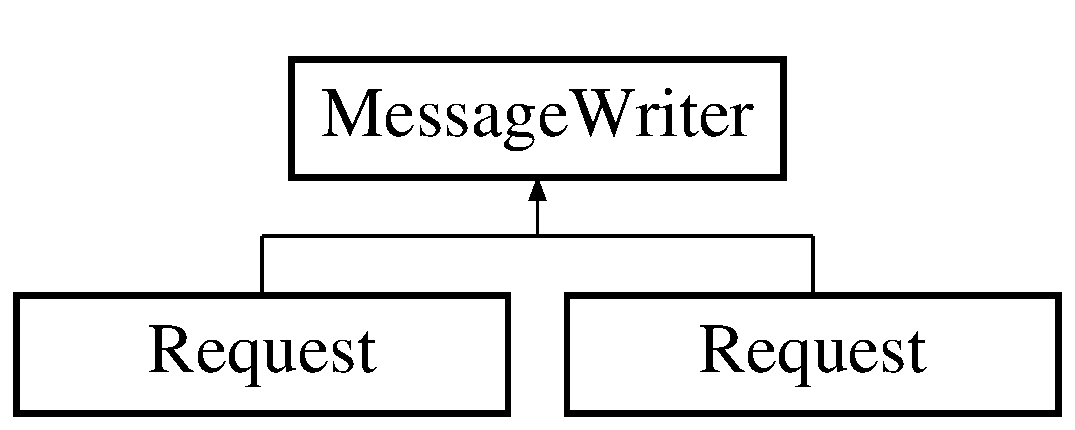
\includegraphics[height=2.000000cm]{class_message_writer}
\end{center}
\end{figure}
\subsection*{Public Member Functions}
\begin{DoxyCompactItemize}
\item 
\hyperlink{class_message_writer_a92f4d619f9ef47dee6237d2826ab6b18}{Message\+Writer} (boost\+::asio\+::io\+\_\+service \&io, Connection\+Interface\+S\+Ptr conn)
\item 
\mbox{\Hypertarget{class_message_writer_a23d55794db33f0d677505190b65943e8}\label{class_message_writer_a23d55794db33f0d677505190b65943e8}} 
void {\bfseries async\+Write} (Message\+Base\+S\+Ptr msg, Write\+Message\+Callback\+Type cb)
\item 
\mbox{\Hypertarget{class_message_writer_a64ef95415e3dc628ac4033675285511c}\label{class_message_writer_a64ef95415e3dc628ac4033675285511c}} 
void {\bfseries async\+Write} (Message\+Base\+S\+Ptr msg, std\+::string \&body\+\_\+string, Write\+Message\+Callback\+Type cb)
\item 
\mbox{\Hypertarget{class_message_writer_a64f2202b6058d2817de987fa1bab056b}\label{class_message_writer_a64f2202b6058d2817de987fa1bab056b}} 
void {\bfseries async\+Write} (Message\+Base\+S\+Ptr msg, M\+Buffer\+S\+Ptr body\+\_\+mb\+\_\+sptr, Write\+Message\+Callback\+Type cb)
\item 
\mbox{\Hypertarget{class_message_writer_a00aa34b356034fc0c49303c7cac5498e}\label{class_message_writer_a00aa34b356034fc0c49303c7cac5498e}} 
void {\bfseries async\+Write} (Message\+Base\+S\+Ptr msg, Buffer\+Chain\+S\+Ptr body\+\_\+chain\+\_\+sptr, Write\+Message\+Callback\+Type cb)
\item 
\mbox{\Hypertarget{class_message_writer_ae4c41c55e28ed99c5535f859fdae7abf}\label{class_message_writer_ae4c41c55e28ed99c5535f859fdae7abf}} 
void {\bfseries async\+Write\+Headers} (Message\+Base\+S\+Ptr msg, Write\+Headers\+Callback\+Type cb)
\item 
\mbox{\Hypertarget{class_message_writer_a4cab5e912c1cb51d23fa76792b3e6eda}\label{class_message_writer_a4cab5e912c1cb51d23fa76792b3e6eda}} 
void {\bfseries async\+Write\+Body\+Data} (std\+::string \&data, Write\+Body\+Data\+Callback\+Type cb)
\item 
\mbox{\Hypertarget{class_message_writer_ab86abed828afa7fbd30e300c585d1d31}\label{class_message_writer_ab86abed828afa7fbd30e300c585d1d31}} 
void {\bfseries async\+Write\+Body\+Data} (\hyperlink{struct_m_buffer}{M\+Buffer} \&data, Write\+Body\+Data\+Callback\+Type cb)
\item 
\mbox{\Hypertarget{class_message_writer_aaf63ccacfe7b7134e75687ef7d19b48c}\label{class_message_writer_aaf63ccacfe7b7134e75687ef7d19b48c}} 
void {\bfseries async\+Write\+Body\+Data} (Buffer\+Chain\+S\+Ptr chain\+\_\+ptr, Write\+Body\+Data\+Callback\+Type cb)
\item 
\mbox{\Hypertarget{class_message_writer_af7ebe407465a33f2f343fe504bb02642}\label{class_message_writer_af7ebe407465a33f2f343fe504bb02642}} 
void {\bfseries async\+Write\+Body\+Data} (boost\+::asio\+::const\+\_\+buffer data, Write\+Body\+Data\+Callback\+Type cb)
\item 
\mbox{\Hypertarget{class_message_writer_a861b118a4ff445b27e09c43f4cac6bda}\label{class_message_writer_a861b118a4ff445b27e09c43f4cac6bda}} 
void {\bfseries async\+Write\+Trailers} (Message\+Base\+S\+Ptr msg, Async\+Write\+Callback\+Type cb)
\item 
\mbox{\Hypertarget{class_message_writer_ac74abc89b3ad3f2b778e7dbfe60e6a72}\label{class_message_writer_ac74abc89b3ad3f2b778e7dbfe60e6a72}} 
void {\bfseries end} ()
\end{DoxyCompactItemize}
\subsection*{Protected Member Functions}
\begin{DoxyCompactItemize}
\item 
\mbox{\Hypertarget{class_message_writer_adf2d412ea99f1a9a9ae198e98013f0b9}\label{class_message_writer_adf2d412ea99f1a9a9ae198e98013f0b9}} 
void {\bfseries async\+Write\+Full\+Body} (Write\+Message\+Callback\+Type cb)
\item 
\mbox{\Hypertarget{class_message_writer_aa6551bbb8ac0808823df8960a36b87bf}\label{class_message_writer_aa6551bbb8ac0808823df8960a36b87bf}} 
void {\bfseries on\+Write\+Headers} (Marvin\+::\+Error\+Type \&ec)
\item 
\mbox{\Hypertarget{class_message_writer_a5a0e7a5a62a95929e5a832bd48200412}\label{class_message_writer_a5a0e7a5a62a95929e5a832bd48200412}} 
void {\bfseries put\+Headers\+Stuff\+In\+Buffer} ()
\end{DoxyCompactItemize}
\subsection*{Protected Attributes}
\begin{DoxyCompactItemize}
\item 
\mbox{\Hypertarget{class_message_writer_aaf28fbb61f0fc9783fab731d12f06aed}\label{class_message_writer_aaf28fbb61f0fc9783fab731d12f06aed}} 
boost\+::asio\+::io\+\_\+service \& {\bfseries \+\_\+io}
\item 
\mbox{\Hypertarget{class_message_writer_a2fa38a10a98a06bec22a59489f582965}\label{class_message_writer_a2fa38a10a98a06bec22a59489f582965}} 
Connection\+Interface\+S\+Ptr {\bfseries \+\_\+conn}
\item 
\mbox{\Hypertarget{class_message_writer_a6b04facc589bab6acca0c85ba5e481ef}\label{class_message_writer_a6b04facc589bab6acca0c85ba5e481ef}} 
Message\+Base\+S\+Ptr {\bfseries \+\_\+current\+Message}
\item 
\hyperlink{struct_m_buffer}{M\+Buffer} \hyperlink{class_message_writer_a77fcbd1fa4556cb745536c5a1eee6d70}{\+\_\+m\+\_\+header\+\_\+buf}
\item 
\mbox{\Hypertarget{class_message_writer_a8a3c2444eb3fd4634a8d1e286fce272d}\label{class_message_writer_a8a3c2444eb3fd4634a8d1e286fce272d}} 
bool {\bfseries \+\_\+have\+Content}
\item 
\mbox{\Hypertarget{class_message_writer_af0bccbe32eecf55f98461ffdd795aac3}\label{class_message_writer_af0bccbe32eecf55f98461ffdd795aac3}} 
boost\+::asio\+::streambuf {\bfseries \+\_\+body\+Buf}
\item 
\mbox{\Hypertarget{class_message_writer_a9a5a72be97d50ee812d04394e138f628}\label{class_message_writer_a9a5a72be97d50ee812d04394e138f628}} 
M\+Buffer\+S\+Ptr {\bfseries \+\_\+body\+\_\+mbuffer\+\_\+sptr}
\item 
\mbox{\Hypertarget{class_message_writer_a3ef2348f35aeeb1d95c5aeb0d037976e}\label{class_message_writer_a3ef2348f35aeeb1d95c5aeb0d037976e}} 
std\+::string {\bfseries \+\_\+body\+\_\+buffer\+\_\+string}
\item 
\mbox{\Hypertarget{class_message_writer_a151a30d9725e35d4c25dcc000a247570}\label{class_message_writer_a151a30d9725e35d4c25dcc000a247570}} 
Buffer\+Chain\+S\+Ptr {\bfseries \+\_\+body\+\_\+buffer\+\_\+chain\+\_\+sptr}
\end{DoxyCompactItemize}
\subsection*{Friends}
\begin{DoxyCompactItemize}
\item 
\mbox{\Hypertarget{class_message_writer_a3740b08ba1b836dbf6a6ca2d3e4fadf7}\label{class_message_writer_a3740b08ba1b836dbf6a6ca2d3e4fadf7}} 
std\+::string {\bfseries trace\+Writer} (\hyperlink{class_message_writer}{Message\+Writer} \&wrtr)
\end{DoxyCompactItemize}


\subsection{Constructor \& Destructor Documentation}
\mbox{\Hypertarget{class_message_writer_a92f4d619f9ef47dee6237d2826ab6b18}\label{class_message_writer_a92f4d619f9ef47dee6237d2826ab6b18}} 
\index{Message\+Writer@{Message\+Writer}!Message\+Writer@{Message\+Writer}}
\index{Message\+Writer@{Message\+Writer}!Message\+Writer@{Message\+Writer}}
\subsubsection{\texorpdfstring{Message\+Writer()}{MessageWriter()}}
{\footnotesize\ttfamily Message\+Writer\+::\+Message\+Writer (\begin{DoxyParamCaption}\item[{boost\+::asio\+::io\+\_\+service \&}]{io,  }\item[{Connection\+Interface\+S\+Ptr}]{conn }\end{DoxyParamCaption})}

The message writer has the logic to output \hyperlink{class_message_base}{Message\+Base} objects to an allready open connection. This is a one-\/shot object -\/ once it has written a single message it should be discarded and a new one used for the next message on the same connection 

\subsection{Member Data Documentation}
\mbox{\Hypertarget{class_message_writer_a77fcbd1fa4556cb745536c5a1eee6d70}\label{class_message_writer_a77fcbd1fa4556cb745536c5a1eee6d70}} 
\index{Message\+Writer@{Message\+Writer}!\+\_\+m\+\_\+header\+\_\+buf@{\+\_\+m\+\_\+header\+\_\+buf}}
\index{\+\_\+m\+\_\+header\+\_\+buf@{\+\_\+m\+\_\+header\+\_\+buf}!Message\+Writer@{Message\+Writer}}
\subsubsection{\texorpdfstring{\+\_\+m\+\_\+header\+\_\+buf}{\_m\_header\_buf}}
{\footnotesize\ttfamily \hyperlink{struct_m_buffer}{M\+Buffer} Message\+Writer\+::\+\_\+m\+\_\+header\+\_\+buf\hspace{0.3cm}{\ttfamily [protected]}}

\begin{DoxyRefDesc}{Todo}
\item[\hyperlink{todo__todo000001}{Todo}]
\begin{DoxyItemize}
\item raw pointers for \hyperlink{struct_m_buffer}{M\+Buffer} and \hyperlink{class_f_buffer}{F\+Buffer} are a problem 
\end{DoxyItemize}\end{DoxyRefDesc}


The documentation for this class was generated from the following files\+:\begin{DoxyCompactItemize}
\item 
marvin/message/message\+\_\+writer.\+hpp\item 
marvin/message/message\+\_\+writer.\+cpp\end{DoxyCompactItemize}

\hypertarget{class_objc_collector}{}\section{Objc\+Collector Class Reference}
\label{class_objc_collector}\index{Objc\+Collector@{Objc\+Collector}}


{\ttfamily \#include $<$objc\+\_\+collector.\+hpp$>$}

\subsection*{Public Member Functions}
\begin{DoxyCompactItemize}
\item 
\hyperlink{class_objc_collector_a8648b6ea89441339da4f8386b3132fdf}{Objc\+Collector} (\hyperlink{class_objc_collector}{Objc\+Collector} const \&)=delete
\item 
\mbox{\Hypertarget{class_objc_collector_aa4b5f226cb4ae0af76a5e86e235add12}\label{class_objc_collector_aa4b5f226cb4ae0af76a5e86e235add12}} 
void {\bfseries operator=} (\hyperlink{class_objc_collector}{Objc\+Collector} const \&)=delete
\item 
void \hyperlink{class_objc_collector_a9518ac372bd2ef1d765bb715730c1f6c}{collect} (std\+::string \&scheme, std\+::string \&host, Message\+Reader\+S\+Ptr req, Message\+Writer\+S\+Ptr resp)
\end{DoxyCompactItemize}
\subsection*{Static Public Member Functions}
\begin{DoxyCompactItemize}
\item 
\mbox{\Hypertarget{class_objc_collector_a95ca99de538f642d4eb4fb01a8dee3b4}\label{class_objc_collector_a95ca99de538f642d4eb4fb01a8dee3b4}} 
static \hyperlink{class_objc_collector}{Objc\+Collector} $\ast$ {\bfseries get\+Instance} (boost\+::asio\+::io\+\_\+service \&io)
\item 
\mbox{\Hypertarget{class_objc_collector_afe187c7f7caebabcd3b6faebbdab71e9}\label{class_objc_collector_afe187c7f7caebabcd3b6faebbdab71e9}} 
static void {\bfseries set\+Delegate} (void $\ast$delegate)
\end{DoxyCompactItemize}
\subsection*{Static Public Attributes}
\begin{DoxyCompactItemize}
\item 
\mbox{\Hypertarget{class_objc_collector_a3b76feca4dba6fa500115a8731e5bbdf}\label{class_objc_collector_a3b76feca4dba6fa500115a8731e5bbdf}} 
static bool {\bfseries \+\_\+first\+Time} = true
\item 
\mbox{\Hypertarget{class_objc_collector_af04ba5a0277f3b48b7fb7c2f0a56f684}\label{class_objc_collector_af04ba5a0277f3b48b7fb7c2f0a56f684}} 
static \hyperlink{class_objc_collector}{Objc\+Collector} $\ast$ {\bfseries \+\_\+instance} = N\+U\+LL
\item 
\mbox{\Hypertarget{class_objc_collector_a31d2f9e91e62e9346e6a496a95dce8ee}\label{class_objc_collector_a31d2f9e91e62e9346e6a496a95dce8ee}} 
static void $\ast$ {\bfseries \+\_\+anon\+Delegate} = N\+U\+LL
\end{DoxyCompactItemize}


\subsection{Detailed Description}
This class is a singleton, but it must be given a reference to the servers io\+\_\+service object so that it can schedule callbacks. Have decided to pass the io\+\_\+service in the static get\+Instance method so that this cannot be forgotten 

\subsection{Constructor \& Destructor Documentation}
\mbox{\Hypertarget{class_objc_collector_a8648b6ea89441339da4f8386b3132fdf}\label{class_objc_collector_a8648b6ea89441339da4f8386b3132fdf}} 
\index{Objc\+Collector@{Objc\+Collector}!Objc\+Collector@{Objc\+Collector}}
\index{Objc\+Collector@{Objc\+Collector}!Objc\+Collector@{Objc\+Collector}}
\subsubsection{\texorpdfstring{Objc\+Collector()}{ObjcCollector()}}
{\footnotesize\ttfamily Objc\+Collector\+::\+Objc\+Collector (\begin{DoxyParamCaption}\item[{\hyperlink{class_objc_collector}{Objc\+Collector} const \&}]{ }\end{DoxyParamCaption})\hspace{0.3cm}{\ttfamily [delete]}}

Delete copy constructors 

\subsection{Member Function Documentation}
\mbox{\Hypertarget{class_objc_collector_a9518ac372bd2ef1d765bb715730c1f6c}\label{class_objc_collector_a9518ac372bd2ef1d765bb715730c1f6c}} 
\index{Objc\+Collector@{Objc\+Collector}!collect@{collect}}
\index{collect@{collect}!Objc\+Collector@{Objc\+Collector}}
\subsubsection{\texorpdfstring{collect()}{collect()}}
{\footnotesize\ttfamily void Objc\+Collector\+::collect (\begin{DoxyParamCaption}\item[{std\+::string \&}]{scheme,  }\item[{std\+::string \&}]{host,  }\item[{Message\+Reader\+S\+Ptr}]{req,  }\item[{Message\+Writer\+S\+Ptr}]{resp }\end{DoxyParamCaption})}

Interface method for client code to call collect In here implement the creation the summary records but dont do any IO or sending leave that for posted\+Collect

The documentation for this class was generated from the following files\+:\begin{DoxyCompactItemize}
\item 
marvin/objc/objc\+\_\+collector.\+hpp\item 
marvin/objc/objc\+\_\+\+\_\+collector.\+mm\end{DoxyCompactItemize}

\hypertarget{class_parser}{}\section{Parser Class Reference}
\label{class_parser}\index{Parser@{Parser}}
Inheritance diagram for Parser\+:\begin{figure}[H]
\begin{center}
\leavevmode
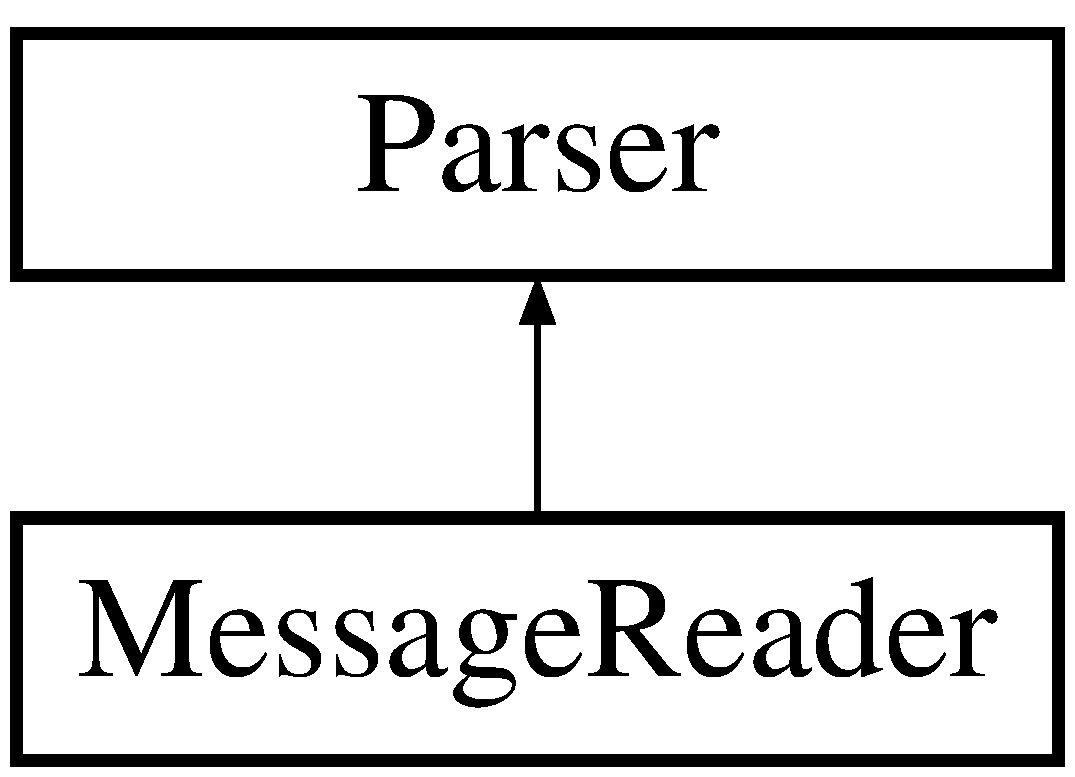
\includegraphics[height=2.000000cm]{class_parser}
\end{center}
\end{figure}
\subsection*{Public Member Functions}
\begin{DoxyCompactItemize}
\item 
void \hyperlink{class_parser_ac6eba4f77cd89023b2940e46ed449df3}{set\+Streaming\+Option} (bool streaming\+Option)
\item 
int \hyperlink{class_parser_a72709d4b733b6ad615669726f77ca52a}{append\+Bytes} (void $\ast$buffer, unsigned length)
\item 
void \hyperlink{class_parser_ac569347a4bdd7a04ede0c0a4c6efe215}{append\+E\+OF} ()
\item 
void \hyperlink{class_parser_a534e9326567306cdf50a7bb980292c37}{pause} ()
\item 
\mbox{\Hypertarget{class_parser_a4872223c0f89b4f6f01eb2af4ab61849}\label{class_parser_a4872223c0f89b4f6f01eb2af4ab61849}} 
void {\bfseries un\+Pause} ()
\item 
\mbox{\Hypertarget{class_parser_af5678187dc7ea87e789b137b65719775}\label{class_parser_af5678187dc7ea87e789b137b65719775}} 
bool {\bfseries is\+Paused} ()
\item 
bool \hyperlink{class_parser_aae7788cc722b8455e691a14dded5d726}{is\+Finished\+Headers} ()
\item 
bool \hyperlink{class_parser_ad9d6c98af922409a78ff65083b1983e3}{is\+Finished\+Message} ()
\item 
\mbox{\Hypertarget{class_parser_a22a7239a764b6f9bd34c044ce1f6bbe2}\label{class_parser_a22a7239a764b6f9bd34c044ce1f6bbe2}} 
bool {\bfseries is\+Error} ()
\item 
\mbox{\Hypertarget{class_parser_ab1701b88c2232d03e1dfc77a7e4b1563}\label{class_parser_ab1701b88c2232d03e1dfc77a7e4b1563}} 
enum http\+\_\+errno {\bfseries get\+Errno} ()
\item 
\mbox{\Hypertarget{class_parser_a293570156f767bf0050fc7889b65f356}\label{class_parser_a293570156f767bf0050fc7889b65f356}} 
\hyperlink{struct_parser_error}{Parser\+Error} {\bfseries get\+Error} ()
\item 
virtual \hyperlink{class_message_interface}{Message\+Interface} $\ast$ \hyperlink{class_parser_a7b3c3ac1cf86a5f9fdda1ecf06dcd4dc}{current\+Message} ()=0
\item 
\mbox{\Hypertarget{class_parser_a543fbd3286c6ca53ed364f4be75473ff}\label{class_parser_a543fbd3286c6ca53ed364f4be75473ff}} 
virtual void {\bfseries On\+Parse\+Begin} ()
\item 
\mbox{\Hypertarget{class_parser_ae1c3a1139dbf03130e4a8c6232bc0f1c}\label{class_parser_ae1c3a1139dbf03130e4a8c6232bc0f1c}} 
virtual void {\bfseries On\+Headers\+Complete} (\hyperlink{class_message_interface}{Message\+Interface} $\ast$msg, void $\ast$body\+\_\+start\+\_\+ptr, std\+::size\+\_\+t remainder)
\item 
\mbox{\Hypertarget{class_parser_a8cd09a2975183aeabc46f492291d10ba}\label{class_parser_a8cd09a2975183aeabc46f492291d10ba}} 
virtual void {\bfseries On\+Message\+Complete} (\hyperlink{class_message_interface}{Message\+Interface} $\ast$msg)
\item 
\mbox{\Hypertarget{class_parser_a721ea9e9c80070e4b41e664329f0c4a4}\label{class_parser_a721ea9e9c80070e4b41e664329f0c4a4}} 
virtual void {\bfseries On\+Parse\+Error} ()
\item 
\mbox{\Hypertarget{class_parser_ab8c3d57fb793c4a5799020e474b7f6f7}\label{class_parser_ab8c3d57fb793c4a5799020e474b7f6f7}} 
virtual void {\bfseries On\+Body\+Data} (void $\ast$buf, int len)
\item 
\mbox{\Hypertarget{class_parser_aba88a1d565dffa2c4845bb74e4e8b09e}\label{class_parser_aba88a1d565dffa2c4845bb74e4e8b09e}} 
virtual void {\bfseries On\+Chunk\+Begin} (int chunk\+Length)
\item 
\mbox{\Hypertarget{class_parser_ab6b2ca1970700b5d1ac9a87cb2bf2776}\label{class_parser_ab6b2ca1970700b5d1ac9a87cb2bf2776}} 
virtual void {\bfseries On\+Chunk\+Data} (void $\ast$buf, int len)
\item 
\mbox{\Hypertarget{class_parser_af755405a007c893d17f2179b06152eda}\label{class_parser_af755405a007c893d17f2179b06152eda}} 
virtual void {\bfseries On\+Chunk\+End} ()
\item 
\mbox{\Hypertarget{class_parser_af14d6a9a94ce9c59690a432571dbc371}\label{class_parser_af14d6a9a94ce9c59690a432571dbc371}} 
void {\bfseries set\+Up\+Parser\+Callbacks} ()
\item 
\mbox{\Hypertarget{class_parser_a34cc536f1137eeadca5ab67c681355aa}\label{class_parser_a34cc536f1137eeadca5ab67c681355aa}} 
void {\bfseries set\+Up\+Next\+Message} ()
\end{DoxyCompactItemize}
\subsection*{Protected Attributes}
\begin{DoxyCompactItemize}
\item 
\mbox{\Hypertarget{class_parser_ad4e7e322f9a17b8339d83186f74a694c}\label{class_parser_ad4e7e322f9a17b8339d83186f74a694c}} 
http\+\_\+parser $\ast$ {\bfseries parser}
\item 
\mbox{\Hypertarget{class_parser_abcf9c5ff429254103942871e829930f5}\label{class_parser_abcf9c5ff429254103942871e829930f5}} 
http\+\_\+parser\+\_\+settings $\ast$ {\bfseries parser\+Settings}
\item 
\mbox{\Hypertarget{class_parser_aadbd6809527f07a8a54a7d9b2520e9ed}\label{class_parser_aadbd6809527f07a8a54a7d9b2520e9ed}} 
bool {\bfseries headers\+Complete\+Flag}
\item 
\mbox{\Hypertarget{class_parser_a1caf934e3135f3c608c7a461ade4db8b}\label{class_parser_a1caf934e3135f3c608c7a461ade4db8b}} 
bool {\bfseries message\+Complete\+Flag}
\item 
\mbox{\Hypertarget{class_parser_a1bdfdb9108621ff22ebe8d6a3f297d2d}\label{class_parser_a1bdfdb9108621ff22ebe8d6a3f297d2d}} 
std\+::string {\bfseries message\+Data}
\item 
\mbox{\Hypertarget{class_parser_aa111be7074c6a7e23475b18329f31b1d}\label{class_parser_aa111be7074c6a7e23475b18329f31b1d}} 
int {\bfseries header\+\_\+state}
\item 
\mbox{\Hypertarget{class_parser_a2a07f1e555ffed364d2e8e9db57cd423}\label{class_parser_a2a07f1e555ffed364d2e8e9db57cd423}} 
simple\+\_\+buffer\+\_\+t $\ast$ {\bfseries url\+\_\+buf}
\item 
\mbox{\Hypertarget{class_parser_a49632afe07eeaf50e025ec7e3a3066d6}\label{class_parser_a49632afe07eeaf50e025ec7e3a3066d6}} 
simple\+\_\+buffer\+\_\+t $\ast$ {\bfseries status\+\_\+buf}
\item 
\mbox{\Hypertarget{class_parser_a9bffeb646e67684de79189570a3d9bd6}\label{class_parser_a9bffeb646e67684de79189570a3d9bd6}} 
simple\+\_\+buffer\+\_\+t $\ast$ {\bfseries name\+\_\+buf}
\item 
\mbox{\Hypertarget{class_parser_abaf2ea297ca47df80116d24c94acd9a2}\label{class_parser_abaf2ea297ca47df80116d24c94acd9a2}} 
simple\+\_\+buffer\+\_\+t $\ast$ {\bfseries value\+\_\+buf}
\item 
\mbox{\Hypertarget{class_parser_a673a3369ac06cbc967394cdd2c441c90}\label{class_parser_a673a3369ac06cbc967394cdd2c441c90}} 
std\+::map$<$ std\+::string, std\+::string $>$ {\bfseries headers}
\end{DoxyCompactItemize}
\subsection*{Friends}
\begin{DoxyCompactItemize}
\item 
\mbox{\Hypertarget{class_parser_a9726af2e5828a3562c0fd11b5ac26c44}\label{class_parser_a9726af2e5828a3562c0fd11b5ac26c44}} 
void {\bfseries save\+Name\+Value\+Pair} (http\+\_\+parser $\ast$parser, simple\+\_\+buffer\+\_\+t $\ast$name, simple\+\_\+buffer\+\_\+t $\ast$value)
\item 
\mbox{\Hypertarget{class_parser_af30ac5f51242b2b1799be52420bac286}\label{class_parser_af30ac5f51242b2b1799be52420bac286}} 
\hyperlink{class_parser}{Parser} $\ast$ {\bfseries get\+Parser} (http\+\_\+parser $\ast$parser)
\item 
\mbox{\Hypertarget{class_parser_a553cdbecb83388bcb98eccddac9af8fa}\label{class_parser_a553cdbecb83388bcb98eccddac9af8fa}} 
void {\bfseries set\+Parser} (http\+\_\+parser $\ast$c\+\_\+parser, \hyperlink{class_parser}{Parser} $\ast$cpp\+\_\+parser)
\item 
\mbox{\Hypertarget{class_parser_a4d73dd1c39e6ea25e3d0ca7eca36b241}\label{class_parser_a4d73dd1c39e6ea25e3d0ca7eca36b241}} 
int {\bfseries message\+\_\+begin\+\_\+cb} (http\+\_\+parser $\ast$parser)
\item 
\mbox{\Hypertarget{class_parser_a30193b3f5c1dc5af2675d6d31e343e8a}\label{class_parser_a30193b3f5c1dc5af2675d6d31e343e8a}} 
int {\bfseries url\+\_\+data\+\_\+cb} (http\+\_\+parser $\ast$parser, const char $\ast$at, size\+\_\+t length)
\item 
\mbox{\Hypertarget{class_parser_a62661f27c58fe69011a1016bf29138ce}\label{class_parser_a62661f27c58fe69011a1016bf29138ce}} 
int {\bfseries status\+\_\+data\+\_\+cb} (http\+\_\+parser $\ast$parser, const char $\ast$at, size\+\_\+t length)
\item 
\mbox{\Hypertarget{class_parser_aaae17943dd3f7db938ec5a1f8c9c8d9b}\label{class_parser_aaae17943dd3f7db938ec5a1f8c9c8d9b}} 
int {\bfseries header\+\_\+field\+\_\+data\+\_\+cb} (http\+\_\+parser $\ast$parser, const char $\ast$at, size\+\_\+t length)
\item 
\mbox{\Hypertarget{class_parser_aa28d460926c10a8f055916842c8eef23}\label{class_parser_aa28d460926c10a8f055916842c8eef23}} 
int {\bfseries header\+\_\+value\+\_\+data\+\_\+cb} (http\+\_\+parser $\ast$parser, const char $\ast$at, size\+\_\+t length)
\item 
\mbox{\Hypertarget{class_parser_afaf8bbeac4baa4f0d275635735f3ed8b}\label{class_parser_afaf8bbeac4baa4f0d275635735f3ed8b}} 
int {\bfseries headers\+\_\+complete\+\_\+cb} (http\+\_\+parser $\ast$parser, const char $\ast$aptr, size\+\_\+t remainder)
\item 
\mbox{\Hypertarget{class_parser_a6a11778033c82b51021c9f7af6796d49}\label{class_parser_a6a11778033c82b51021c9f7af6796d49}} 
int {\bfseries chunk\+\_\+size\+\_\+start} (http\+\_\+parser $\ast$parser, const char $\ast$at, size\+\_\+t length)
\item 
\mbox{\Hypertarget{class_parser_ac54638bfd9ba21a338f3ed6decd587c9}\label{class_parser_ac54638bfd9ba21a338f3ed6decd587c9}} 
int {\bfseries chunk\+\_\+header\+\_\+cb} (http\+\_\+parser $\ast$parser)
\item 
\mbox{\Hypertarget{class_parser_a63771c42c64eca8eb6ebaba249a241de}\label{class_parser_a63771c42c64eca8eb6ebaba249a241de}} 
int {\bfseries body\+\_\+data\+\_\+cb} (http\+\_\+parser $\ast$parser, const char $\ast$at, size\+\_\+t length)
\item 
\mbox{\Hypertarget{class_parser_a9944899a787daa6ff1a03c3c8db106ac}\label{class_parser_a9944899a787daa6ff1a03c3c8db106ac}} 
int {\bfseries chunk\+\_\+complete\+\_\+cb} (http\+\_\+parser $\ast$parser)
\item 
\mbox{\Hypertarget{class_parser_a74c8ba05a16748266ea355b8fe4d1626}\label{class_parser_a74c8ba05a16748266ea355b8fe4d1626}} 
int {\bfseries message\+\_\+complete\+\_\+cb} (http\+\_\+parser $\ast$parser)
\end{DoxyCompactItemize}


\subsection{Member Function Documentation}
\mbox{\Hypertarget{class_parser_a72709d4b733b6ad615669726f77ca52a}\label{class_parser_a72709d4b733b6ad615669726f77ca52a}} 
\index{Parser@{Parser}!append\+Bytes@{append\+Bytes}}
\index{append\+Bytes@{append\+Bytes}!Parser@{Parser}}
\subsubsection{\texorpdfstring{append\+Bytes()}{appendBytes()}}
{\footnotesize\ttfamily int Parser\+::append\+Bytes (\begin{DoxyParamCaption}\item[{void $\ast$}]{buffer,  }\item[{unsigned}]{length }\end{DoxyParamCaption})}

send data to the parser for consumption \mbox{\Hypertarget{class_parser_ac569347a4bdd7a04ede0c0a4c6efe215}\label{class_parser_ac569347a4bdd7a04ede0c0a4c6efe215}} 
\index{Parser@{Parser}!append\+E\+OF@{append\+E\+OF}}
\index{append\+E\+OF@{append\+E\+OF}!Parser@{Parser}}
\subsubsection{\texorpdfstring{append\+E\+O\+F()}{appendEOF()}}
{\footnotesize\ttfamily void Parser\+::append\+E\+OF (\begin{DoxyParamCaption}{ }\end{DoxyParamCaption})}

Signal end of data to the parser. Required in some cases as there are message formats that do not contain message length information. \mbox{\Hypertarget{class_parser_a7b3c3ac1cf86a5f9fdda1ecf06dcd4dc}\label{class_parser_a7b3c3ac1cf86a5f9fdda1ecf06dcd4dc}} 
\index{Parser@{Parser}!current\+Message@{current\+Message}}
\index{current\+Message@{current\+Message}!Parser@{Parser}}
\subsubsection{\texorpdfstring{current\+Message()}{currentMessage()}}
{\footnotesize\ttfamily virtual \hyperlink{class_message_interface}{Message\+Interface}$\ast$ Parser\+::current\+Message (\begin{DoxyParamCaption}{ }\end{DoxyParamCaption})\hspace{0.3cm}{\ttfamily [pure virtual]}}

Returns the the Message currently being parsed. When operating in non streaming mode this also returns the most recently parsed message. 

Implemented in \hyperlink{class_message_reader_a06ec9e561ff5cde8f4e1ffb0ff17cb1f}{Message\+Reader}.

\mbox{\Hypertarget{class_parser_aae7788cc722b8455e691a14dded5d726}\label{class_parser_aae7788cc722b8455e691a14dded5d726}} 
\index{Parser@{Parser}!is\+Finished\+Headers@{is\+Finished\+Headers}}
\index{is\+Finished\+Headers@{is\+Finished\+Headers}!Parser@{Parser}}
\subsubsection{\texorpdfstring{is\+Finished\+Headers()}{isFinishedHeaders()}}
{\footnotesize\ttfamily bool Parser\+::is\+Finished\+Headers (\begin{DoxyParamCaption}{ }\end{DoxyParamCaption})}

return true if parsing of the header fields of the current message is finished. In which case the header fields can be obtained thru the headers property of the \hyperlink{class_h_t_t_p_message}{H\+T\+T\+P\+Message} returned from $\ast$ get\+Current\+Message \mbox{\Hypertarget{class_parser_ad9d6c98af922409a78ff65083b1983e3}\label{class_parser_ad9d6c98af922409a78ff65083b1983e3}} 
\index{Parser@{Parser}!is\+Finished\+Message@{is\+Finished\+Message}}
\index{is\+Finished\+Message@{is\+Finished\+Message}!Parser@{Parser}}
\subsubsection{\texorpdfstring{is\+Finished\+Message()}{isFinishedMessage()}}
{\footnotesize\ttfamily bool Parser\+::is\+Finished\+Message (\begin{DoxyParamCaption}{ }\end{DoxyParamCaption})}

return true if parsing of current message is finished, in which case the message can be obtained via the get\+Current\+Message method \mbox{\Hypertarget{class_parser_a534e9326567306cdf50a7bb980292c37}\label{class_parser_a534e9326567306cdf50a7bb980292c37}} 
\index{Parser@{Parser}!pause@{pause}}
\index{pause@{pause}!Parser@{Parser}}
\subsubsection{\texorpdfstring{pause()}{pause()}}
{\footnotesize\ttfamily void Parser\+::pause (\begin{DoxyParamCaption}{ }\end{DoxyParamCaption})}

Pause and/or unpause the parser \mbox{\Hypertarget{class_parser_ac6eba4f77cd89023b2940e46ed449df3}\label{class_parser_ac6eba4f77cd89023b2940e46ed449df3}} 
\index{Parser@{Parser}!set\+Streaming\+Option@{set\+Streaming\+Option}}
\index{set\+Streaming\+Option@{set\+Streaming\+Option}!Parser@{Parser}}
\subsubsection{\texorpdfstring{set\+Streaming\+Option()}{setStreamingOption()}}
{\footnotesize\ttfamily void Parser\+::set\+Streaming\+Option (\begin{DoxyParamCaption}\item[{bool}]{streaming\+Option }\end{DoxyParamCaption})}

Sets the message streaming option -\/ to the value of stream\+Option 

The documentation for this class was generated from the following files\+:\begin{DoxyCompactItemize}
\item 
marvin/message/parser.\+hpp\item 
marvin/message/parser.\+cpp\end{DoxyCompactItemize}

\hypertarget{struct_parser_error}{}\section{Parser\+Error Struct Reference}
\label{struct_parser_error}\index{Parser\+Error@{Parser\+Error}}
\subsection*{Public Attributes}
\begin{DoxyCompactItemize}
\item 
\mbox{\Hypertarget{struct_parser_error_ade2aea99ef35e168080b364b44669d8a}\label{struct_parser_error_ade2aea99ef35e168080b364b44669d8a}} 
std\+::string {\bfseries name}
\item 
\mbox{\Hypertarget{struct_parser_error_a98c65694d3655ecef0626e6f57322646}\label{struct_parser_error_a98c65694d3655ecef0626e6f57322646}} 
std\+::string {\bfseries description}
\item 
\mbox{\Hypertarget{struct_parser_error_a2f4e2b18fb1f7097ca4751875e589fa7}\label{struct_parser_error_a2f4e2b18fb1f7097ca4751875e589fa7}} 
enum http\+\_\+errno {\bfseries err\+\_\+number}
\end{DoxyCompactItemize}


The documentation for this struct was generated from the following file\+:\begin{DoxyCompactItemize}
\item 
marvin/message/parser.\+hpp\end{DoxyCompactItemize}

\hypertarget{class_pipe_collector}{}\section{Pipe\+Collector Class Reference}
\label{class_pipe_collector}\index{Pipe\+Collector@{Pipe\+Collector}}


{\ttfamily \#include $<$pipe\+\_\+collector.\+hpp$>$}

\subsection*{Public Member Functions}
\begin{DoxyCompactItemize}
\item 
\hyperlink{class_pipe_collector_ad2a04b5f8e95e204cfe1d85bded0c92d}{Pipe\+Collector} (\hyperlink{class_pipe_collector}{Pipe\+Collector} const \&)=delete
\item 
\mbox{\Hypertarget{class_pipe_collector_ae286d157a61dbef510e1903ad245e96e}\label{class_pipe_collector_ae286d157a61dbef510e1903ad245e96e}} 
void {\bfseries operator=} (\hyperlink{class_pipe_collector}{Pipe\+Collector} const \&)=delete
\item 
void \hyperlink{class_pipe_collector_a4deab58d1636c9af54146df61f4d244c}{collect} (std\+::string \&scheme, std\+::string \&host, Message\+Reader\+S\+Ptr req, Message\+Writer\+S\+Ptr resp)
\end{DoxyCompactItemize}
\subsection*{Static Public Member Functions}
\begin{DoxyCompactItemize}
\item 
\mbox{\Hypertarget{class_pipe_collector_ad5f10086bc650dc13a1b620c2c425edb}\label{class_pipe_collector_ad5f10086bc650dc13a1b620c2c425edb}} 
static \hyperlink{class_pipe_collector}{Pipe\+Collector} $\ast$ {\bfseries get\+Instance} (boost\+::asio\+::io\+\_\+service \&io)
\item 
\mbox{\Hypertarget{class_pipe_collector_ab2b95b11b4910616abff4846fe291064}\label{class_pipe_collector_ab2b95b11b4910616abff4846fe291064}} 
static void {\bfseries config\+Set\+\_\+\+Pipe\+Path} (std\+::string path)
\end{DoxyCompactItemize}
\subsection*{Static Public Attributes}
\begin{DoxyCompactItemize}
\item 
\mbox{\Hypertarget{class_pipe_collector_ab599c19550e7b7d2534231c9e9d61375}\label{class_pipe_collector_ab599c19550e7b7d2534231c9e9d61375}} 
static bool {\bfseries \+\_\+first\+Time} = true
\item 
\mbox{\Hypertarget{class_pipe_collector_af8c74d185ce54c2193ec8f42ef099698}\label{class_pipe_collector_af8c74d185ce54c2193ec8f42ef099698}} 
static \hyperlink{class_pipe_collector}{Pipe\+Collector} $\ast$ {\bfseries \+\_\+instance} = N\+U\+LL
\item 
\mbox{\Hypertarget{class_pipe_collector_a1bbb1d5bd4d23738cc0e90e0a8644f55}\label{class_pipe_collector_a1bbb1d5bd4d23738cc0e90e0a8644f55}} 
static std\+::string {\bfseries \+\_\+pipe\+Path} = \char`\"{}\char`\"{}
\end{DoxyCompactItemize}


\subsection{Detailed Description}
This class is a singleton that requires to be primed with the servers io\+\_\+service object so that it (this class) can schedule callbacks. I chose to have the io\+\_\+service passed in the get\+Instance static method, that way cannot forget

In addition it needs the path name of the pipe to which it will write. That should be set via the static method config\+Set\+\_\+\+Pipe\+Path during the startup phase of the server.

This class also has a boost strand to protect against mutiple access to critical sections of code. B\+UT, this class also does synchronous stream IO which will delay whatever thread the strand is running on to prevent this delaying the entire proxy process the server should start an additional thread and connect it to the geneal io\+\_\+service to aleviate this issue. 

\subsection{Constructor \& Destructor Documentation}
\mbox{\Hypertarget{class_pipe_collector_ad2a04b5f8e95e204cfe1d85bded0c92d}\label{class_pipe_collector_ad2a04b5f8e95e204cfe1d85bded0c92d}} 
\index{Pipe\+Collector@{Pipe\+Collector}!Pipe\+Collector@{Pipe\+Collector}}
\index{Pipe\+Collector@{Pipe\+Collector}!Pipe\+Collector@{Pipe\+Collector}}
\subsubsection{\texorpdfstring{Pipe\+Collector()}{PipeCollector()}}
{\footnotesize\ttfamily Pipe\+Collector\+::\+Pipe\+Collector (\begin{DoxyParamCaption}\item[{\hyperlink{class_pipe_collector}{Pipe\+Collector} const \&}]{ }\end{DoxyParamCaption})\hspace{0.3cm}{\ttfamily [delete]}}

Delete copy constructors 

\subsection{Member Function Documentation}
\mbox{\Hypertarget{class_pipe_collector_a4deab58d1636c9af54146df61f4d244c}\label{class_pipe_collector_a4deab58d1636c9af54146df61f4d244c}} 
\index{Pipe\+Collector@{Pipe\+Collector}!collect@{collect}}
\index{collect@{collect}!Pipe\+Collector@{Pipe\+Collector}}
\subsubsection{\texorpdfstring{collect()}{collect()}}
{\footnotesize\ttfamily void Pipe\+Collector\+::collect (\begin{DoxyParamCaption}\item[{std\+::string \&}]{scheme,  }\item[{std\+::string \&}]{host,  }\item[{Message\+Reader\+S\+Ptr}]{req,  }\item[{Message\+Writer\+S\+Ptr}]{resp }\end{DoxyParamCaption})}

Interface method for client code to call collect In here implement the creation the summary records but dont do any IO or sending leave that for posted\+Collect

The documentation for this class was generated from the following files\+:\begin{DoxyCompactItemize}
\item 
marvin/collector/pipe\+\_\+collector.\+hpp\item 
marvin/collector/pipe\+\_\+collector.\+cpp\end{DoxyCompactItemize}

\hypertarget{class_read_socket_interface}{}\section{Read\+Socket\+Interface Class Reference}
\label{class_read_socket_interface}\index{Read\+Socket\+Interface@{Read\+Socket\+Interface}}
Inheritance diagram for Read\+Socket\+Interface\+:\begin{figure}[H]
\begin{center}
\leavevmode
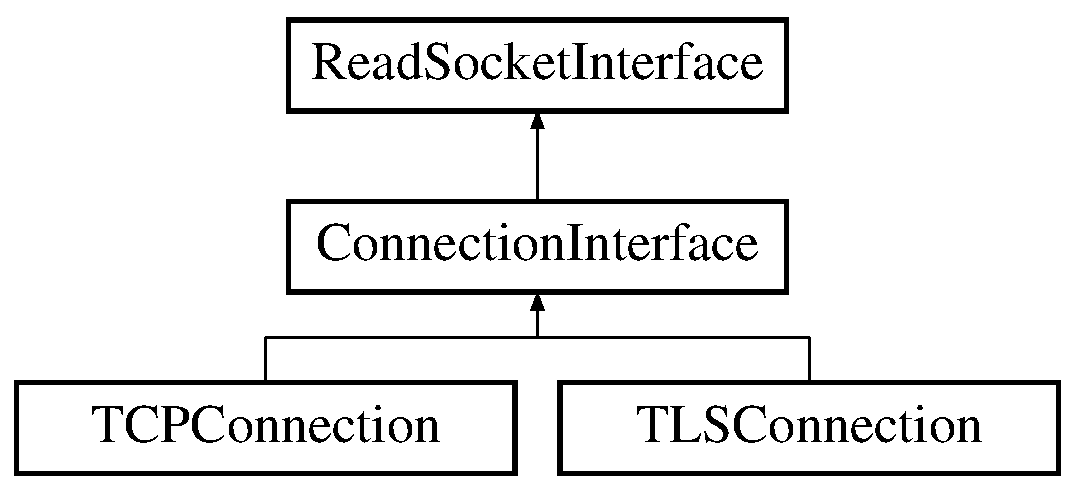
\includegraphics[height=3.000000cm]{class_read_socket_interface}
\end{center}
\end{figure}
\subsection*{Public Member Functions}
\begin{DoxyCompactItemize}
\item 
\mbox{\Hypertarget{class_read_socket_interface_a012ec2a7ec7b6b1142e8e1a808e27442}\label{class_read_socket_interface_a012ec2a7ec7b6b1142e8e1a808e27442}} 
virtual void {\bfseries async\+Read} (\hyperlink{struct_m_buffer}{M\+Buffer} \&mb, Async\+Read\+Callback cb)=0
\item 
\mbox{\Hypertarget{class_read_socket_interface_a51b24e615ebc0d887585affcc9d269af}\label{class_read_socket_interface_a51b24e615ebc0d887585affcc9d269af}} 
virtual long {\bfseries native\+Socket\+FD} ()=0
\end{DoxyCompactItemize}


The documentation for this class was generated from the following file\+:\begin{DoxyCompactItemize}
\item 
marvin/include/read\+\_\+socket\+\_\+interface.\+hpp\end{DoxyCompactItemize}

\hypertarget{class_request}{}\section{Request Class Reference}
\label{class_request}\index{Request@{Request}}
Inheritance diagram for Request\+:\begin{figure}[H]
\begin{center}
\leavevmode
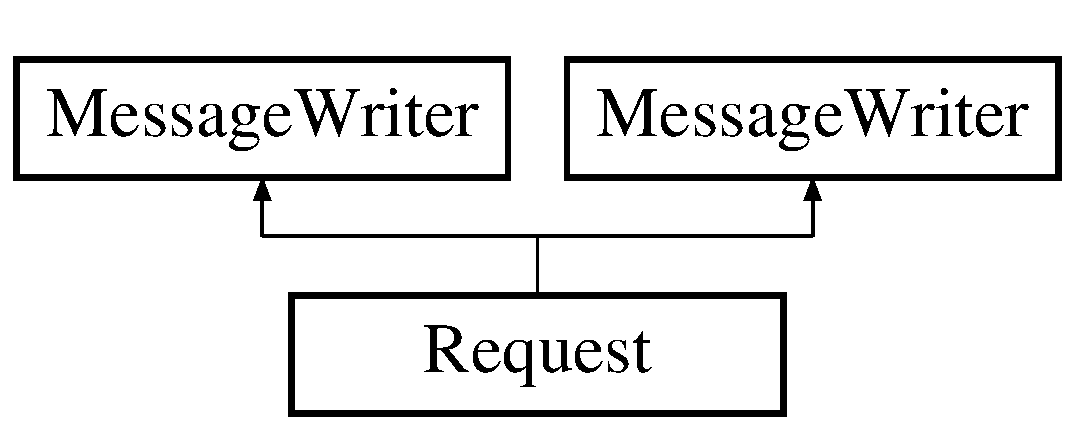
\includegraphics[height=2.000000cm]{class_request}
\end{center}
\end{figure}
\subsection*{Public Member Functions}
\begin{DoxyCompactItemize}
\item 
\mbox{\Hypertarget{class_request_a94f71ef02d2d80f134e3a83064b66589}\label{class_request_a94f71ef02d2d80f134e3a83064b66589}} 
{\bfseries Request} (boost\+::asio\+::io\+\_\+service \&io)
\item 
\mbox{\Hypertarget{class_request_aaea4c25d9eef0985a1e5dd57a5b29633}\label{class_request_aaea4c25d9eef0985a1e5dd57a5b29633}} 
{\bfseries Request} (const \hyperlink{class_request}{Request} \&other)=delete
\item 
\mbox{\Hypertarget{class_request_ad7fb0a96230a4f6f778d636a1a0b0335}\label{class_request_ad7fb0a96230a4f6f778d636a1a0b0335}} 
\hyperlink{class_request}{Request} \& {\bfseries operator=} (const \hyperlink{class_request}{Request} \&)=delete
\item 
\mbox{\Hypertarget{class_request_a181c57295b0a5e2f28b1845f9d605260}\label{class_request_a181c57295b0a5e2f28b1845f9d605260}} 
void {\bfseries go} (std\+::function$<$ void(Marvin\+::\+Error\+Type \&err)$>$ cb)
\item 
\hyperlink{class_message_reader}{Message\+Reader} \& \hyperlink{class_request_ac9e91894d06fac3bcb657ba64693da22}{get\+Response} ()
\item 
void \hyperlink{class_request_a0a0cc1ae66771dd92c1ad78e9e6df59a}{set\+Url} (std\+::string url)
\item 
\mbox{\Hypertarget{class_request_a34a6c9ee0d9789a98950e3146c42db14}\label{class_request_a34a6c9ee0d9789a98950e3146c42db14}} 
void {\bfseries end} ()
\item 
\mbox{\Hypertarget{class_request_a94f71ef02d2d80f134e3a83064b66589}\label{class_request_a94f71ef02d2d80f134e3a83064b66589}} 
{\bfseries Request} (boost\+::asio\+::io\+\_\+service \&io)
\item 
\mbox{\Hypertarget{class_request_aaea4c25d9eef0985a1e5dd57a5b29633}\label{class_request_aaea4c25d9eef0985a1e5dd57a5b29633}} 
{\bfseries Request} (const \hyperlink{class_request}{Request} \&other)=delete
\item 
\mbox{\Hypertarget{class_request_ad7fb0a96230a4f6f778d636a1a0b0335}\label{class_request_ad7fb0a96230a4f6f778d636a1a0b0335}} 
\hyperlink{class_request}{Request} \& {\bfseries operator=} (const \hyperlink{class_request}{Request} \&)=delete
\item 
\mbox{\Hypertarget{class_request_a181c57295b0a5e2f28b1845f9d605260}\label{class_request_a181c57295b0a5e2f28b1845f9d605260}} 
void {\bfseries go} (std\+::function$<$ void(Marvin\+::\+Error\+Type \&err)$>$ cb)
\item 
\mbox{\Hypertarget{class_request_a367164dedd048b63c542ad028bade31b}\label{class_request_a367164dedd048b63c542ad028bade31b}} 
\hyperlink{class_message_reader}{Message\+Reader} \& {\bfseries get\+Response} ()
\item 
\mbox{\Hypertarget{class_request_a0a0cc1ae66771dd92c1ad78e9e6df59a}\label{class_request_a0a0cc1ae66771dd92c1ad78e9e6df59a}} 
void {\bfseries set\+Url} (std\+::string url)
\item 
\mbox{\Hypertarget{class_request_a34a6c9ee0d9789a98950e3146c42db14}\label{class_request_a34a6c9ee0d9789a98950e3146c42db14}} 
void {\bfseries end} ()
\end{DoxyCompactItemize}
\subsection*{Protected Member Functions}
\begin{DoxyCompactItemize}
\item 
\mbox{\Hypertarget{class_request_ad6d505e24ef5b1038d5820d3541df091}\label{class_request_ad6d505e24ef5b1038d5820d3541df091}} 
void {\bfseries async\+Get\+Write\+Socket} (Connect\+Callback\+Type connect\+Cb)
\item 
\mbox{\Hypertarget{class_request_a79a3f10ae291bd48c7b7664d7a7c5419}\label{class_request_a79a3f10ae291bd48c7b7664d7a7c5419}} 
void {\bfseries have\+Connection} (Marvin\+::\+Error\+Type \&err, \hyperlink{class_connection_interface}{Connection\+Interface} $\ast$conn)
\item 
\mbox{\Hypertarget{class_request_a03ba174751dad7a36ce9706f9a067aa0}\label{class_request_a03ba174751dad7a36ce9706f9a067aa0}} 
void {\bfseries full\+Write\+Handler} (Marvin\+::\+Error\+Type \&err)
\item 
\mbox{\Hypertarget{class_request_aff1b5c9d9b7760186179ec5cb911d2a4}\label{class_request_aff1b5c9d9b7760186179ec5cb911d2a4}} 
void {\bfseries read\+Complete} (Marvin\+::\+Error\+Type \&err)
\item 
\mbox{\Hypertarget{class_request_abebb155c39c86a63113f1998a7cb28d6}\label{class_request_abebb155c39c86a63113f1998a7cb28d6}} 
void {\bfseries default\+Headers} ()
\end{DoxyCompactItemize}
\subsection*{Protected Attributes}
\begin{DoxyCompactItemize}
\item 
\mbox{\Hypertarget{class_request_a281495472bc533384d273ad2e9c747b7}\label{class_request_a281495472bc533384d273ad2e9c747b7}} 
boost\+::asio\+::io\+\_\+service \& {\bfseries \+\_\+io}
\item 
\mbox{\Hypertarget{class_request_a384fc425224362988597830b21d9a48e}\label{class_request_a384fc425224362988597830b21d9a48e}} 
Message\+Reader\+S\+Ptr {\bfseries \+\_\+rdr}
\item 
\mbox{\Hypertarget{class_request_a1fc82297ae22708d0c405c422c66807f}\label{class_request_a1fc82297ae22708d0c405c422c66807f}} 
Connection\+Interface\+S\+Ptr {\bfseries \+\_\+connection}
\item 
\mbox{\Hypertarget{class_request_aa9852adbf9fba98ba7bdecb6e8d5a30e}\label{class_request_aa9852adbf9fba98ba7bdecb6e8d5a30e}} 
Read\+Socket\+Interface\+S\+Ptr {\bfseries \+\_\+read\+Sock}
\item 
\mbox{\Hypertarget{class_request_a1a605eca637460576d0f56d3c8c7b936}\label{class_request_a1a605eca637460576d0f56d3c8c7b936}} 
std\+::function$<$ void(Marvin\+::\+Error\+Type \&err)$>$ {\bfseries \+\_\+go\+Cb}
\item 
\mbox{\Hypertarget{class_request_ae6cf259304098272c26655851aa482cd}\label{class_request_ae6cf259304098272c26655851aa482cd}} 
bool {\bfseries \+\_\+one\+Trip\+Only}
\item 
\mbox{\Hypertarget{class_request_a6e689919d384805d52ebfd2f8fec71db}\label{class_request_a6e689919d384805d52ebfd2f8fec71db}} 
std\+::string {\bfseries \+\_\+service}
\item 
\mbox{\Hypertarget{class_request_acaef6cea153579e81bad5bd5da7922f8}\label{class_request_acaef6cea153579e81bad5bd5da7922f8}} 
std\+::string {\bfseries \+\_\+server}
\item 
\mbox{\Hypertarget{class_request_a967d7538ddd207dfb720881f2258566a}\label{class_request_a967d7538ddd207dfb720881f2258566a}} 
std\+::string {\bfseries \+\_\+scheme}
\item 
\mbox{\Hypertarget{class_request_ad2eaec63a9e7259713435c6c07f2f2a1}\label{class_request_ad2eaec63a9e7259713435c6c07f2f2a1}} 
std\+::string {\bfseries \+\_\+host}
\item 
\mbox{\Hypertarget{class_request_a921b319801626a6de3efcd7105449c2b}\label{class_request_a921b319801626a6de3efcd7105449c2b}} 
std\+::string {\bfseries \+\_\+port}
\item 
\mbox{\Hypertarget{class_request_a0cbbe7e1f72e983934815780bffd679a}\label{class_request_a0cbbe7e1f72e983934815780bffd679a}} 
std\+::string {\bfseries \+\_\+path}
\item 
\mbox{\Hypertarget{class_request_ac087de88773edb3045709a5a5a480fa0}\label{class_request_ac087de88773edb3045709a5a5a480fa0}} 
Url\+::\+Query {\bfseries \+\_\+query}
\item 
\mbox{\Hypertarget{class_request_ad5911146df93fe3b6ea57b0ca5280880}\label{class_request_ad5911146df93fe3b6ea57b0ca5280880}} 
std\+::string {\bfseries \+\_\+query\+Str}
\end{DoxyCompactItemize}
\subsection*{Friends}
\begin{DoxyCompactItemize}
\item 
\mbox{\Hypertarget{class_request_aafeb39491c604dd3ba954b382d31f56f}\label{class_request_aafeb39491c604dd3ba954b382d31f56f}} 
std\+::string {\bfseries trace\+Request} (\hyperlink{class_request}{Request} \&request)
\end{DoxyCompactItemize}


\subsection{Member Function Documentation}
\mbox{\Hypertarget{class_request_ac9e91894d06fac3bcb657ba64693da22}\label{class_request_ac9e91894d06fac3bcb657ba64693da22}} 
\index{Request@{Request}!get\+Response@{get\+Response}}
\index{get\+Response@{get\+Response}!Request@{Request}}
\subsubsection{\texorpdfstring{get\+Response()}{getResponse()}}
{\footnotesize\ttfamily \hyperlink{class_message_reader}{Message\+Reader} \& Request\+::get\+Response (\begin{DoxyParamCaption}{ }\end{DoxyParamCaption})}



 \subsubsection*{getter for the response message inside this request }\mbox{\Hypertarget{class_request_a0a0cc1ae66771dd92c1ad78e9e6df59a}\label{class_request_a0a0cc1ae66771dd92c1ad78e9e6df59a}} 
\index{Request@{Request}!set\+Url@{set\+Url}}
\index{set\+Url@{set\+Url}!Request@{Request}}
\subsubsection{\texorpdfstring{set\+Url()}{setUrl()}}
{\footnotesize\ttfamily void Request\+::set\+Url (\begin{DoxyParamCaption}\item[{std\+::string}]{url }\end{DoxyParamCaption})}



 sets the url for the request, parses the url into components and saves them in particular deduces
\begin{DoxyItemize}
\item scheme
\item host -\/ both with and without port appended
\item port
\item path/uri \subsubsection*{-\/ query string }
\end{DoxyItemize}

The documentation for this class was generated from the following files\+:\begin{DoxyCompactItemize}
\item 
marvin/client/request.\+hpp\item 
marvin/src/request copy.\+hpp\item 
marvin/client/request.\+cpp\item 
marvin/src/request copy.\+cpp\end{DoxyCompactItemize}

\hypertarget{class_request_handler}{}\section{Request\+Handler Class Reference}
\label{class_request_handler}\index{Request\+Handler@{Request\+Handler}}


The common handler for all incoming requests.  




{\ttfamily \#include $<$request\+\_\+handler.\+hpp$>$}

Inheritance diagram for Request\+Handler\+:\begin{figure}[H]
\begin{center}
\leavevmode
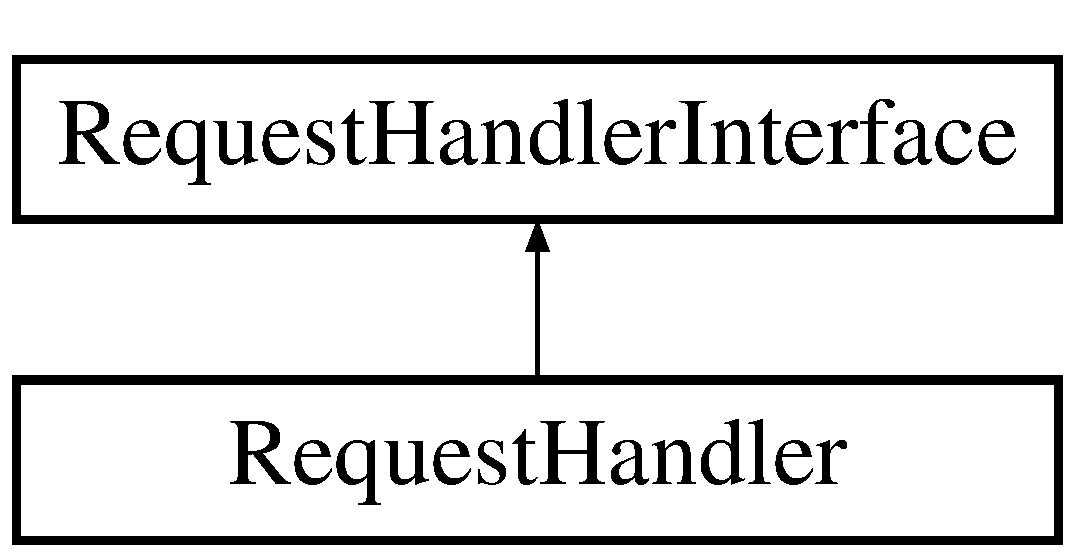
\includegraphics[height=2.000000cm]{class_request_handler}
\end{center}
\end{figure}
\subsection*{Public Member Functions}
\begin{DoxyCompactItemize}
\item 
\mbox{\Hypertarget{class_request_handler_a7dc4f72ed63d826b58e8d5702a552287}\label{class_request_handler_a7dc4f72ed63d826b58e8d5702a552287}} 
{\bfseries Request\+Handler} (const \hyperlink{class_request_handler}{Request\+Handler} \&)=delete
\item 
\mbox{\Hypertarget{class_request_handler_a72a2ff62932e8ac74a5fe55415eff602}\label{class_request_handler_a72a2ff62932e8ac74a5fe55415eff602}} 
\hyperlink{class_request_handler}{Request\+Handler} \& {\bfseries operator=} (const \hyperlink{class_request_handler}{Request\+Handler} \&)=delete
\item 
\mbox{\Hypertarget{class_request_handler_ad8326a61b01339812eb11f2905f2407c}\label{class_request_handler_ad8326a61b01339812eb11f2905f2407c}} 
\hyperlink{class_request_handler_ad8326a61b01339812eb11f2905f2407c}{Request\+Handler} (const std\+::string \&doc\+\_\+root)
\begin{DoxyCompactList}\small\item\em Construct with a directory containing files to be served. \end{DoxyCompactList}\item 
\mbox{\Hypertarget{class_request_handler_ae7870b58bbff92ebab452e715a1f0121}\label{class_request_handler_ae7870b58bbff92ebab452e715a1f0121}} 
void \hyperlink{class_request_handler_ae7870b58bbff92ebab452e715a1f0121}{handle\+\_\+request} (const request \&req, reply \&rep)
\begin{DoxyCompactList}\small\item\em Handle a request and produce a reply. \end{DoxyCompactList}\end{DoxyCompactItemize}


\subsection{Detailed Description}
The common handler for all incoming requests. 

The documentation for this class was generated from the following files\+:\begin{DoxyCompactItemize}
\item 
marvin/src/request\+\_\+handler.\+hpp\item 
marvin/src/request\+\_\+handler.\+cpp\end{DoxyCompactItemize}

\hypertarget{class_request_handler_base}{}\section{Request\+Handler\+Base Class Reference}
\label{class_request_handler_base}\index{Request\+Handler\+Base@{Request\+Handler\+Base}}
Inheritance diagram for Request\+Handler\+Base\+:\begin{figure}[H]
\begin{center}
\leavevmode
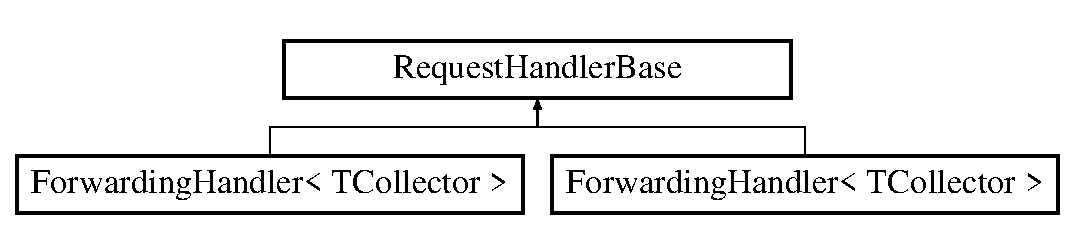
\includegraphics[height=2.000000cm]{class_request_handler_base}
\end{center}
\end{figure}
\subsection*{Public Member Functions}
\begin{DoxyCompactItemize}
\item 
\mbox{\Hypertarget{class_request_handler_base_af49294d2f3435b9618738e3f9d62e34d}\label{class_request_handler_base_af49294d2f3435b9618738e3f9d62e34d}} 
{\bfseries Request\+Handler\+Base} (boost\+::asio\+::io\+\_\+service \&io)
\item 
\mbox{\Hypertarget{class_request_handler_base_a0864015433e1c4001bd820b3f9127c65}\label{class_request_handler_base_a0864015433e1c4001bd820b3f9127c65}} 
virtual void {\bfseries handle\+Connect} (\hyperlink{struct_server_context}{Server\+Context} \&server\+\_\+context, Message\+Reader\+S\+Ptr req, Connection\+Interface\+S\+Ptr conn\+Ptr, Handler\+Done\+Callback\+Type done)
\item 
\mbox{\Hypertarget{class_request_handler_base_a4aafaf3189fd47439d4636dbf830f3e6}\label{class_request_handler_base_a4aafaf3189fd47439d4636dbf830f3e6}} 
virtual void {\bfseries handle\+Request} (\hyperlink{struct_server_context}{Server\+Context} \&server\+\_\+context, Message\+Reader\+S\+Ptr req, Message\+Writer\+S\+Ptr rep, Handler\+Done\+Callback\+Type done)=0
\end{DoxyCompactItemize}
\subsection*{Protected Attributes}
\begin{DoxyCompactItemize}
\item 
\mbox{\Hypertarget{class_request_handler_base_a7dc27fb1e0097c2bdc3dc4060e9d9c87}\label{class_request_handler_base_a7dc27fb1e0097c2bdc3dc4060e9d9c87}} 
boost\+::asio\+::io\+\_\+service \& {\bfseries \+\_\+io}
\end{DoxyCompactItemize}


The documentation for this class was generated from the following files\+:\begin{DoxyCompactItemize}
\item 
marvin/server/request\+\_\+handler\+\_\+base.\+hpp\item 
marvin/server/request\+\_\+handler\+\_\+base.\+cpp\end{DoxyCompactItemize}

\hypertarget{class_server_connection_manager}{}\section{Server\+Connection\+Manager Class Reference}
\label{class_server_connection_manager}\index{Server\+Connection\+Manager@{Server\+Connection\+Manager}}
\subsection*{Public Types}
\begin{DoxyCompactItemize}
\item 
\mbox{\Hypertarget{class_server_connection_manager_a28eaf417682341e6f8c733b30c59bbd8}\label{class_server_connection_manager_a28eaf417682341e6f8c733b30c59bbd8}} 
typedef std\+::function$<$ void()$>$ {\bfseries Allow\+Another\+Callback}
\end{DoxyCompactItemize}
\subsection*{Public Member Functions}
\begin{DoxyCompactItemize}
\item 
\mbox{\Hypertarget{class_server_connection_manager_a8f20818d0fd29612ce09f694aaad0271}\label{class_server_connection_manager_a8f20818d0fd29612ce09f694aaad0271}} 
{\bfseries Server\+Connection\+Manager} (const \hyperlink{class_server_connection_manager}{Server\+Connection\+Manager} \&)=delete
\item 
\mbox{\Hypertarget{class_server_connection_manager_a3193017398278086cb7d79820987c5e2}\label{class_server_connection_manager_a3193017398278086cb7d79820987c5e2}} 
\hyperlink{class_server_connection_manager}{Server\+Connection\+Manager} \& {\bfseries operator=} (const \hyperlink{class_server_connection_manager}{Server\+Connection\+Manager} \&)=delete
\item 
\hyperlink{class_server_connection_manager_a0b2c91c8c5f07706cbec0bb08de8039d}{Server\+Connection\+Manager} (boost\+::asio\+::io\+\_\+service \&io, boost\+::asio\+::strand \&server\+Strand, int max\+\_\+connections)
\item 
void \hyperlink{class_server_connection_manager_a9661756cbecdbec901860ffec5cf6e47}{allow\+Another\+Connection} (Allow\+Another\+Callback cb)
\item 
void \hyperlink{class_server_connection_manager_aa2c03c50b5154af1424ed92a35cd6389}{register\+Connection\+Handler} (\hyperlink{class_connection_handler}{Connection\+Handler} $\ast$conn\+Handler)
\item 
void \hyperlink{class_server_connection_manager_a61073d71f21045b5202fa035e9da282f}{deregister} (\hyperlink{class_connection_handler}{Connection\+Handler} $\ast$ch)
\item 
void \hyperlink{class_server_connection_manager_a83a3b22ce780b4762ad06e7f2ffbb611}{stop\+\_\+all} ()
\end{DoxyCompactItemize}
\subsection*{Static Public Member Functions}
\begin{DoxyCompactItemize}
\item 
\mbox{\Hypertarget{class_server_connection_manager_a548c5d053584a2a0bf18a1422a802b95}\label{class_server_connection_manager_a548c5d053584a2a0bf18a1422a802b95}} 
static \hyperlink{class_server_connection_manager}{Server\+Connection\+Manager} $\ast$ {\bfseries get\+\_\+instance} ()
\item 
\mbox{\Hypertarget{class_server_connection_manager_a2aabc84134814ff480b8214bda06cb26}\label{class_server_connection_manager_a2aabc84134814ff480b8214bda06cb26}} 
static bool {\bfseries verify} ()
\end{DoxyCompactItemize}
\subsection*{Static Public Attributes}
\begin{DoxyCompactItemize}
\item 
\mbox{\Hypertarget{class_server_connection_manager_a79204557e4949379c3197dd476d74ccb}\label{class_server_connection_manager_a79204557e4949379c3197dd476d74ccb}} 
static \hyperlink{class_server_connection_manager}{Server\+Connection\+Manager} $\ast$ {\bfseries instance}
\end{DoxyCompactItemize}


\subsection{Constructor \& Destructor Documentation}
\mbox{\Hypertarget{class_server_connection_manager_a0b2c91c8c5f07706cbec0bb08de8039d}\label{class_server_connection_manager_a0b2c91c8c5f07706cbec0bb08de8039d}} 
\index{Server\+Connection\+Manager@{Server\+Connection\+Manager}!Server\+Connection\+Manager@{Server\+Connection\+Manager}}
\index{Server\+Connection\+Manager@{Server\+Connection\+Manager}!Server\+Connection\+Manager@{Server\+Connection\+Manager}}
\subsubsection{\texorpdfstring{Server\+Connection\+Manager()}{ServerConnectionManager()}}
{\footnotesize\ttfamily Server\+Connection\+Manager\+::\+Server\+Connection\+Manager (\begin{DoxyParamCaption}\item[{boost\+::asio\+::io\+\_\+service \&}]{io,  }\item[{boost\+::asio\+::strand \&}]{server\+Strand,  }\item[{int}]{max\+\_\+connections }\end{DoxyParamCaption})}

Construct a connection manager. The connection handler must operate in a single threaded manner. That is achieved by requiring it to always execute on the server strand. 

\subsection{Member Function Documentation}
\mbox{\Hypertarget{class_server_connection_manager_a9661756cbecdbec901860ffec5cf6e47}\label{class_server_connection_manager_a9661756cbecdbec901860ffec5cf6e47}} 
\index{Server\+Connection\+Manager@{Server\+Connection\+Manager}!allow\+Another\+Connection@{allow\+Another\+Connection}}
\index{allow\+Another\+Connection@{allow\+Another\+Connection}!Server\+Connection\+Manager@{Server\+Connection\+Manager}}
\subsubsection{\texorpdfstring{allow\+Another\+Connection()}{allowAnotherConnection()}}
{\footnotesize\ttfamily void Server\+Connection\+Manager\+::allow\+Another\+Connection (\begin{DoxyParamCaption}\item[{Server\+Connection\+Manager\+::\+Allow\+Another\+Callback}]{cb }\end{DoxyParamCaption})}

called by server to verify that another accept is permitted within the context of the Connection\+Manager\textquotesingle{}s rescource allocation scheme. If not the Connection\+Manager will wait till there is enough resource and invoke the cb to signal the server to continue. Did it this was so that the Connection\+Manager does not need to know how to create \hyperlink{class_connection_handler}{Connection\+Handler}, \hyperlink{class_request_handler}{Request\+Handler} \mbox{\Hypertarget{class_server_connection_manager_a61073d71f21045b5202fa035e9da282f}\label{class_server_connection_manager_a61073d71f21045b5202fa035e9da282f}} 
\index{Server\+Connection\+Manager@{Server\+Connection\+Manager}!deregister@{deregister}}
\index{deregister@{deregister}!Server\+Connection\+Manager@{Server\+Connection\+Manager}}
\subsubsection{\texorpdfstring{deregister()}{deregister()}}
{\footnotesize\ttfamily void Server\+Connection\+Manager\+::deregister (\begin{DoxyParamCaption}\item[{\hyperlink{class_connection_handler}{Connection\+Handler} $\ast$}]{ch }\end{DoxyParamCaption})}

deregister the specified connection, removes from the table and decrements the count of active connection handlers. If the there is a \char`\"{}allow another callback\char`\"{} set invoke this callback if the number of active connection handlers is below the max allowed

This is called from a \hyperlink{class_connection_handler}{Connection\+Handler} running on an arbitary io\+\_\+service. need to post the real action on the server strand. \mbox{\Hypertarget{class_server_connection_manager_aa2c03c50b5154af1424ed92a35cd6389}\label{class_server_connection_manager_aa2c03c50b5154af1424ed92a35cd6389}} 
\index{Server\+Connection\+Manager@{Server\+Connection\+Manager}!register\+Connection\+Handler@{register\+Connection\+Handler}}
\index{register\+Connection\+Handler@{register\+Connection\+Handler}!Server\+Connection\+Manager@{Server\+Connection\+Manager}}
\subsubsection{\texorpdfstring{register\+Connection\+Handler()}{registerConnectionHandler()}}
{\footnotesize\ttfamily void Server\+Connection\+Manager\+::register\+Connection\+Handler (\begin{DoxyParamCaption}\item[{\hyperlink{class_connection_handler}{Connection\+Handler} $\ast$}]{conn\+Handler }\end{DoxyParamCaption})}

Register a connection handler in a table so that it stays around to process request/response and increments the count of connection handler active

This method is A\+L\+W\+A\+YS called from the server strand so do not have to post it on that strand. \mbox{\Hypertarget{class_server_connection_manager_a83a3b22ce780b4762ad06e7f2ffbb611}\label{class_server_connection_manager_a83a3b22ce780b4762ad06e7f2ffbb611}} 
\index{Server\+Connection\+Manager@{Server\+Connection\+Manager}!stop\+\_\+all@{stop\+\_\+all}}
\index{stop\+\_\+all@{stop\+\_\+all}!Server\+Connection\+Manager@{Server\+Connection\+Manager}}
\subsubsection{\texorpdfstring{stop\+\_\+all()}{stop\_all()}}
{\footnotesize\ttfamily void Server\+Connection\+Manager\+::stop\+\_\+all (\begin{DoxyParamCaption}{ }\end{DoxyParamCaption})}

Stop all connections. 

The documentation for this class was generated from the following files\+:\begin{DoxyCompactItemize}
\item 
marvin/server/server\+\_\+connection\+\_\+manager.\+hpp\item 
marvin/server/server\+\_\+connection\+\_\+manager.\+cpp\end{DoxyCompactItemize}

\hypertarget{struct_server_context}{}\section{Server\+Context Struct Reference}
\label{struct_server_context}\index{Server\+Context@{Server\+Context}}
\subsection*{Public Attributes}
\begin{DoxyCompactItemize}
\item 
\mbox{\Hypertarget{struct_server_context_ae750155d467495cd07eb5abc04010ffc}\label{struct_server_context_ae750155d467495cd07eb5abc04010ffc}} 
\hyperlink{class_h_t_t_p_server}{H\+T\+T\+P\+Server} $\ast$ {\bfseries server\+\_\+ptr}
\item 
\mbox{\Hypertarget{struct_server_context_ae9559a8d8279579e8fa8d74149bf9afd}\label{struct_server_context_ae9559a8d8279579e8fa8d74149bf9afd}} 
\hyperlink{class_server_connection_manager}{Server\+Connection\+Manager} $\ast$ {\bfseries server\+\_\+connection\+\_\+manager\+\_\+ptr}
\item 
\mbox{\Hypertarget{struct_server_context_a3a9fc04b2e2d874fbfe3582064a1f67d}\label{struct_server_context_a3a9fc04b2e2d874fbfe3582064a1f67d}} 
\hyperlink{class_connection_handler}{Connection\+Handler} $\ast$ {\bfseries connection\+\_\+handler\+\_\+ptr}
\item 
\mbox{\Hypertarget{struct_server_context_ac94fa33cf25884ec14bb1ab887bfe973}\label{struct_server_context_ac94fa33cf25884ec14bb1ab887bfe973}} 
\hyperlink{class_connection_interface}{Connection\+Interface} $\ast$ {\bfseries connection\+\_\+ptr}
\end{DoxyCompactItemize}


The documentation for this struct was generated from the following file\+:\begin{DoxyCompactItemize}
\item 
marvin/server/server\+\_\+context.\+hpp\end{DoxyCompactItemize}

\hypertarget{interface_single_transaction}{}\section{Single\+Transaction Class Reference}
\label{interface_single_transaction}\index{Single\+Transaction@{Single\+Transaction}}
Inheritance diagram for Single\+Transaction\+:\begin{figure}[H]
\begin{center}
\leavevmode
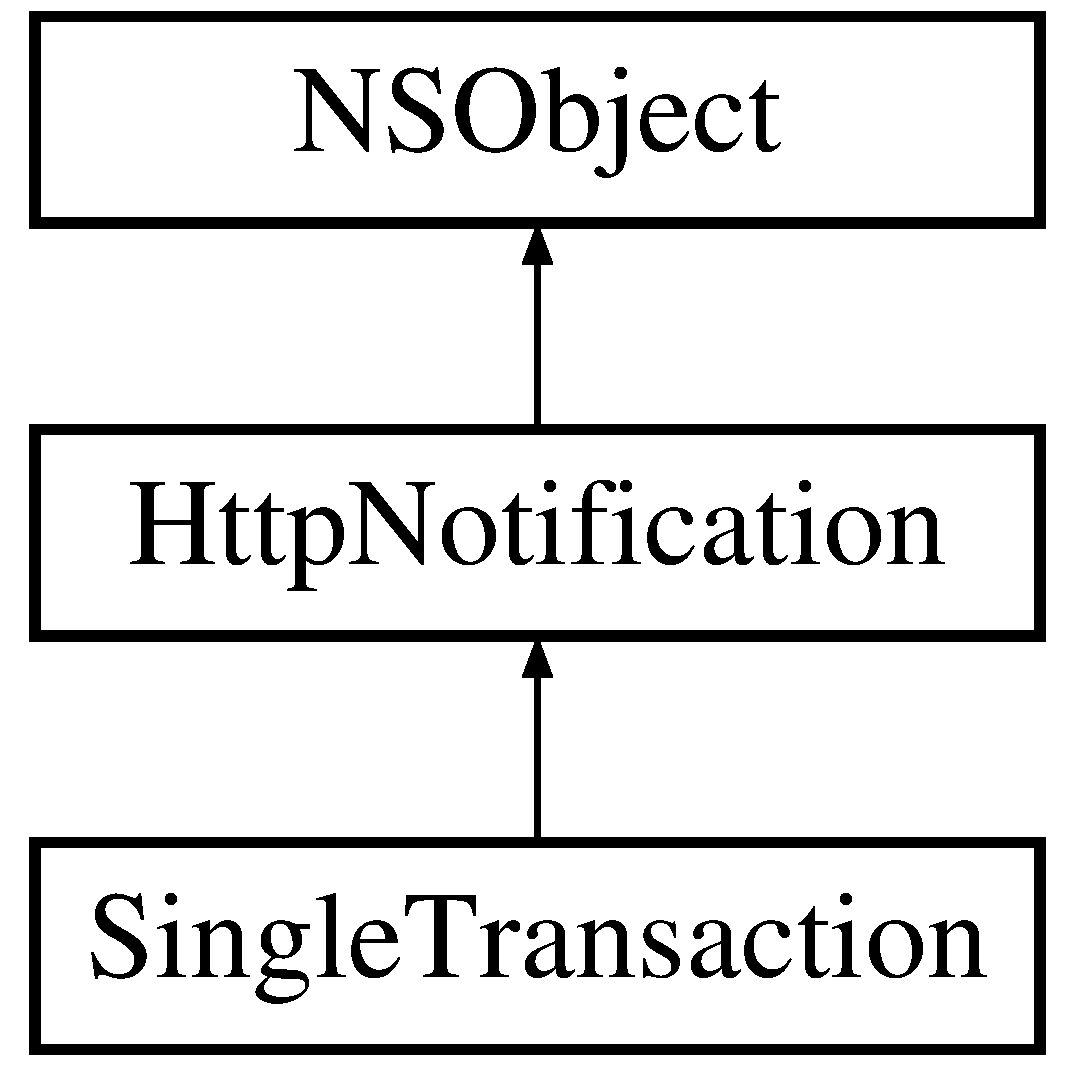
\includegraphics[height=3.000000cm]{interface_single_transaction}
\end{center}
\end{figure}
\subsection*{Additional Inherited Members}


The documentation for this class was generated from the following file\+:\begin{DoxyCompactItemize}
\item 
marvin/objc/traffic/Single\+Transaction.\+h\end{DoxyCompactItemize}

\hypertarget{class_t_c_p_connection}{}\section{T\+C\+P\+Connection Class Reference}
\label{class_t_c_p_connection}\index{T\+C\+P\+Connection@{T\+C\+P\+Connection}}
Inheritance diagram for T\+C\+P\+Connection\+:\begin{figure}[H]
\begin{center}
\leavevmode
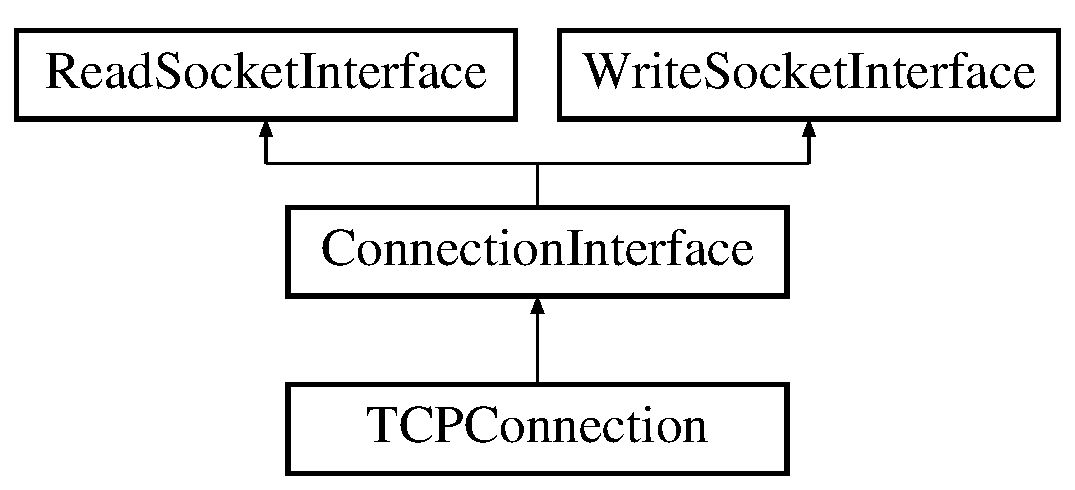
\includegraphics[height=3.000000cm]{class_t_c_p_connection}
\end{center}
\end{figure}
\subsection*{Public Member Functions}
\begin{DoxyCompactItemize}
\item 
\hyperlink{class_t_c_p_connection_a1786a9f9ea84d1e504dee290d0425ce8}{T\+C\+P\+Connection} (boost\+::asio\+::io\+\_\+service \&io\+\_\+service, const std\+::string scheme, const std\+::string server, const std\+::string port)
\item 
\hyperlink{class_t_c_p_connection_af66a3430e661be59609f5cdbd2f19317}{T\+C\+P\+Connection} (boost\+::asio\+::io\+\_\+service \&io\+\_\+service)
\item 
void \hyperlink{class_t_c_p_connection_a4984a896404d02c9dc1135e788a71a4d}{async\+Connect} (Connect\+Callback\+Type cb)
\item 
\mbox{\Hypertarget{class_t_c_p_connection_ab49c7b4120490daec460c9b0bd06dfbd}\label{class_t_c_p_connection_ab49c7b4120490daec460c9b0bd06dfbd}} 
void {\bfseries async\+Accept} (boost\+::asio\+::ip\+::tcp\+::acceptor \&acceptor, std\+::function$<$ void(const boost\+::system\+::error\+\_\+code \&err)$>$ cb)
\item 
void \hyperlink{class_t_c_p_connection_af45c4a0d2feb5faefd2d82505460bf15}{async\+Write} (\hyperlink{struct_m_buffer}{M\+Buffer} \&buffer, Async\+Write\+Callback\+Type cb)
\item 
\mbox{\Hypertarget{class_t_c_p_connection_a39f657137386c99671e5b0bb660ac1ef}\label{class_t_c_p_connection_a39f657137386c99671e5b0bb660ac1ef}} 
void {\bfseries async\+Write} (std\+::string \&str, Async\+Write\+Callback\+Type cb)
\item 
void \hyperlink{class_t_c_p_connection_ad4b619a97387b39d107abfa4c3d9efe5}{async\+Write} (Buffer\+Chain\+S\+Ptr buf\+\_\+chain\+\_\+sptr, Async\+Write\+Callback cb)
\item 
\mbox{\Hypertarget{class_t_c_p_connection_a99e5f8c52d41a365cb8a99cdf7b2e96d}\label{class_t_c_p_connection_a99e5f8c52d41a365cb8a99cdf7b2e96d}} 
void {\bfseries async\+Write} (boost\+::asio\+::const\+\_\+buffer buf, Async\+Write\+Callback cb)
\item 
\mbox{\Hypertarget{class_t_c_p_connection_a2bd787d3f088dcea9d48b993fa043a1c}\label{class_t_c_p_connection_a2bd787d3f088dcea9d48b993fa043a1c}} 
void {\bfseries async\+Write} (boost\+::asio\+::streambuf \&sb, Async\+Write\+Callback)
\item 
void \hyperlink{class_t_c_p_connection_a32fb26d3c6d30c59a5b8c5c7a056b1b9}{async\+Read} (\hyperlink{struct_m_buffer}{M\+Buffer} \&mb, Async\+Read\+Callback\+Type cb)
\item 
\mbox{\Hypertarget{class_t_c_p_connection_afdd912efe436e41d99a60ef1bb16ec73}\label{class_t_c_p_connection_afdd912efe436e41d99a60ef1bb16ec73}} 
void {\bfseries shutdown} ()
\item 
\mbox{\Hypertarget{class_t_c_p_connection_ab9d37f9ec45ee1c1bfb4164aed8b7135}\label{class_t_c_p_connection_ab9d37f9ec45ee1c1bfb4164aed8b7135}} 
void {\bfseries close} ()
\item 
long \hyperlink{class_t_c_p_connection_a76fd32d49d1875e8e4a0f9f503a92bcd}{native\+Socket\+FD} ()
\item 
\mbox{\Hypertarget{class_t_c_p_connection_ac270233abe1610585bcaa86e654cf6ad}\label{class_t_c_p_connection_ac270233abe1610585bcaa86e654cf6ad}} 
std\+::string {\bfseries scheme} ()
\item 
\mbox{\Hypertarget{class_t_c_p_connection_a3dc68d736ab41b8550696f1bdedaf40a}\label{class_t_c_p_connection_a3dc68d736ab41b8550696f1bdedaf40a}} 
std\+::string {\bfseries server} ()
\item 
\mbox{\Hypertarget{class_t_c_p_connection_ac8ed90aa1225fe1f534e736a438ac8bd}\label{class_t_c_p_connection_ac8ed90aa1225fe1f534e736a438ac8bd}} 
std\+::string {\bfseries service} ()
\end{DoxyCompactItemize}
\subsection*{Static Public Member Functions}
\begin{DoxyCompactItemize}
\item 
\mbox{\Hypertarget{class_t_c_p_connection_a55d72a606e2ec9be8e145606001c9790}\label{class_t_c_p_connection_a55d72a606e2ec9be8e145606001c9790}} 
static void {\bfseries set\+Config\+\_\+connect\+Time\+Out} (long millisecs)
\item 
\mbox{\Hypertarget{class_t_c_p_connection_acbf6e8d1866906ce7b1a269c0df35f20}\label{class_t_c_p_connection_acbf6e8d1866906ce7b1a269c0df35f20}} 
static void {\bfseries set\+Config\+\_\+read\+Time\+Out} (long millisecs)
\item 
\mbox{\Hypertarget{class_t_c_p_connection_a1a53971c6eeadf5dd1be0aa45b654694}\label{class_t_c_p_connection_a1a53971c6eeadf5dd1be0aa45b654694}} 
static void {\bfseries set\+Config\+\_\+write\+Time\+Out} (long millisecs)
\item 
\mbox{\Hypertarget{class_t_c_p_connection_a22bdfdfecfdf97f4b8024e28e2ed6eb0}\label{class_t_c_p_connection_a22bdfdfecfdf97f4b8024e28e2ed6eb0}} 
static void {\bfseries fd\+\_\+inuse} (int fd)
\item 
\mbox{\Hypertarget{class_t_c_p_connection_ac0077ddd447c155402fa00348ec8635d}\label{class_t_c_p_connection_ac0077ddd447c155402fa00348ec8635d}} 
static void {\bfseries fd\+\_\+free} (int fd)
\end{DoxyCompactItemize}
\subsection*{Static Public Attributes}
\begin{DoxyCompactItemize}
\item 
static long \hyperlink{class_t_c_p_connection_a20685b25079d961a7a9bf1f35b9e80c9}{\+\_\+\+\_\+connect\+\_\+timeout\+\_\+interval\+\_\+ms} = 5000
\item 
\mbox{\Hypertarget{class_t_c_p_connection_ab556118dc22a172990f22306047eb4f0}\label{class_t_c_p_connection_ab556118dc22a172990f22306047eb4f0}} 
static long {\bfseries \+\_\+\+\_\+read\+\_\+timeout\+\_\+interval\+\_\+ms} = 5000
\item 
\mbox{\Hypertarget{class_t_c_p_connection_adb05ef40de90512600fea00ce229b9ed}\label{class_t_c_p_connection_adb05ef40de90512600fea00ce229b9ed}} 
static long {\bfseries \+\_\+\+\_\+write\+\_\+timeout\+\_\+interval\+\_\+ms} = 5000
\item 
static std\+::map$<$ int, int $>$ \hyperlink{class_t_c_p_connection_a257b53aea1460ce87ca0d5f269d1326f}{socket\+\_\+fds\+\_\+inuse}
\end{DoxyCompactItemize}


\subsection{Constructor \& Destructor Documentation}
\mbox{\Hypertarget{class_t_c_p_connection_a1786a9f9ea84d1e504dee290d0425ce8}\label{class_t_c_p_connection_a1786a9f9ea84d1e504dee290d0425ce8}} 
\index{T\+C\+P\+Connection@{T\+C\+P\+Connection}!T\+C\+P\+Connection@{T\+C\+P\+Connection}}
\index{T\+C\+P\+Connection@{T\+C\+P\+Connection}!T\+C\+P\+Connection@{T\+C\+P\+Connection}}
\subsubsection{\texorpdfstring{T\+C\+P\+Connection()}{TCPConnection()}\hspace{0.1cm}{\footnotesize\ttfamily [1/2]}}
{\footnotesize\ttfamily T\+C\+P\+Connection\+::\+T\+C\+P\+Connection (\begin{DoxyParamCaption}\item[{boost\+::asio\+::io\+\_\+service \&}]{io\+\_\+service,  }\item[{const std\+::string}]{scheme,  }\item[{const std\+::string}]{server,  }\item[{const std\+::string}]{port }\end{DoxyParamCaption})}

client socket needs to know who to connect to 
\begin{DoxyParams}{Parameters}
{\em io\+\_\+service} & io\+\_\+service\& the runloop on which this connection will run \\
\hline
{\em scheme} & std\+::string -\/ values are \char`\"{}http\char`\"{} or \char`\"{}https\char`\"{} \\
\hline
{\em server} & std\+::string -\/ a name such as www.\+google.\+com, N\+O\+TE no port number on the end \\
\hline
{\em port} & std\+::string\\
\hline
\end{DoxyParams}
Constructor 
\begin{DoxyParams}{Parameters}
{\em \{io\+\_\+service\}} & io\+\_\+service -\/ to use for running \\
\hline
{\em \{string\}} & scheme -\/ \char`\"{}http\char`\"{} or \char`\"{}https\char`\"{} \\
\hline
{\em \{string\}} & server -\/ domain string \\
\hline
\end{DoxyParams}
\mbox{\Hypertarget{class_t_c_p_connection_af66a3430e661be59609f5cdbd2f19317}\label{class_t_c_p_connection_af66a3430e661be59609f5cdbd2f19317}} 
\index{T\+C\+P\+Connection@{T\+C\+P\+Connection}!T\+C\+P\+Connection@{T\+C\+P\+Connection}}
\index{T\+C\+P\+Connection@{T\+C\+P\+Connection}!T\+C\+P\+Connection@{T\+C\+P\+Connection}}
\subsubsection{\texorpdfstring{T\+C\+P\+Connection()}{TCPConnection()}\hspace{0.1cm}{\footnotesize\ttfamily [2/2]}}
{\footnotesize\ttfamily T\+C\+P\+Connection\+::\+T\+C\+P\+Connection (\begin{DoxyParamCaption}\item[{boost\+::asio\+::io\+\_\+service \&}]{io\+\_\+service }\end{DoxyParamCaption})}

server socket will be connected via listen/accept 

\subsection{Member Function Documentation}
\mbox{\Hypertarget{class_t_c_p_connection_a4984a896404d02c9dc1135e788a71a4d}\label{class_t_c_p_connection_a4984a896404d02c9dc1135e788a71a4d}} 
\index{T\+C\+P\+Connection@{T\+C\+P\+Connection}!async\+Connect@{async\+Connect}}
\index{async\+Connect@{async\+Connect}!T\+C\+P\+Connection@{T\+C\+P\+Connection}}
\subsubsection{\texorpdfstring{async\+Connect()}{asyncConnect()}}
{\footnotesize\ttfamily void T\+C\+P\+Connection\+::async\+Connect (\begin{DoxyParamCaption}\item[{Connect\+Callback\+Type}]{cb }\end{DoxyParamCaption})\hspace{0.3cm}{\ttfamily [virtual]}}

A Note on timeouts, the use of a boost\+::asio\+::strand by this class, and concurrent calls to the async io methods defined below.


\begin{DoxyEnumerate}
\item Only one async I/O operation should be outstanding at any time.
\item Internally this class applies timeouts to the operations\+:
\begin{DoxyItemize}
\item async\+Connect
\item async\+Read
\item async\+Write in all its forms to accomodate this an instance of boost\+::asio\+::strand is used to ensure that internal io handlers coordinate correctly and do not run concurrently.
\end{DoxyItemize}

H\+Owever all callbacks provided to async\+Connect, async\+Read, async\+Write are scheduled (using \+\_\+io.\+post())on the instance of io\+\_\+service being used by the \hyperlink{class_t_c_p_connection}{T\+C\+P\+Connection} instance and A\+RE N\+OT running on the internal strand. These callbacks should N\+OT be wrapped by another strand as that could cause deadlocks.

Notice that async\+Accept was N\+OT included in the list of io ops subject to timeout. \begin{DoxyVerb}-   asyncAccept is intended to be used by a server and could be outstanding for a very long time,
    and hence a timeout seems inappropriate
-   because of no timeout there is no need for internal handlers associated with asyncAccept
    to be run on the internal asio::strand.
-   it is likely that asyncAccept callback will be wrapped by a strand within a server as part
    of a servers management of its own concurrency issues.\end{DoxyVerb}
 
\end{DoxyEnumerate}

Implements \hyperlink{class_connection_interface}{Connection\+Interface}.

\mbox{\Hypertarget{class_t_c_p_connection_a32fb26d3c6d30c59a5b8c5c7a056b1b9}\label{class_t_c_p_connection_a32fb26d3c6d30c59a5b8c5c7a056b1b9}} 
\index{T\+C\+P\+Connection@{T\+C\+P\+Connection}!async\+Read@{async\+Read}}
\index{async\+Read@{async\+Read}!T\+C\+P\+Connection@{T\+C\+P\+Connection}}
\subsubsection{\texorpdfstring{async\+Read()}{asyncRead()}}
{\footnotesize\ttfamily void T\+C\+P\+Connection\+::async\+Read (\begin{DoxyParamCaption}\item[{\hyperlink{struct_m_buffer}{M\+Buffer} \&}]{buffer,  }\item[{Async\+Read\+Callback\+Type}]{cb }\end{DoxyParamCaption})\hspace{0.3cm}{\ttfamily [virtual]}}

read 

Implements \hyperlink{class_read_socket_interface}{Read\+Socket\+Interface}.

\mbox{\Hypertarget{class_t_c_p_connection_af45c4a0d2feb5faefd2d82505460bf15}\label{class_t_c_p_connection_af45c4a0d2feb5faefd2d82505460bf15}} 
\index{T\+C\+P\+Connection@{T\+C\+P\+Connection}!async\+Write@{async\+Write}}
\index{async\+Write@{async\+Write}!T\+C\+P\+Connection@{T\+C\+P\+Connection}}
\subsubsection{\texorpdfstring{async\+Write()}{asyncWrite()}\hspace{0.1cm}{\footnotesize\ttfamily [1/2]}}
{\footnotesize\ttfamily void T\+C\+P\+Connection\+::async\+Write (\begin{DoxyParamCaption}\item[{\hyperlink{struct_m_buffer}{M\+Buffer} \&}]{buf,  }\item[{Async\+Write\+Callback\+Type}]{cb }\end{DoxyParamCaption})\hspace{0.3cm}{\ttfamily [virtual]}}

write 

Implements \hyperlink{class_connection_interface}{Connection\+Interface}.

\mbox{\Hypertarget{class_t_c_p_connection_ad4b619a97387b39d107abfa4c3d9efe5}\label{class_t_c_p_connection_ad4b619a97387b39d107abfa4c3d9efe5}} 
\index{T\+C\+P\+Connection@{T\+C\+P\+Connection}!async\+Write@{async\+Write}}
\index{async\+Write@{async\+Write}!T\+C\+P\+Connection@{T\+C\+P\+Connection}}
\subsubsection{\texorpdfstring{async\+Write()}{asyncWrite()}\hspace{0.1cm}{\footnotesize\ttfamily [2/2]}}
{\footnotesize\ttfamily void T\+C\+P\+Connection\+::async\+Write (\begin{DoxyParamCaption}\item[{Buffer\+Chain\+S\+Ptr}]{buf\+\_\+chain\+\_\+sptr,  }\item[{Async\+Write\+Callback}]{cb }\end{DoxyParamCaption})\hspace{0.3cm}{\ttfamily [virtual]}}

this took a while to work out -\/ change buffer code at your peril 

Implements \hyperlink{class_connection_interface}{Connection\+Interface}.

\mbox{\Hypertarget{class_t_c_p_connection_a76fd32d49d1875e8e4a0f9f503a92bcd}\label{class_t_c_p_connection_a76fd32d49d1875e8e4a0f9f503a92bcd}} 
\index{T\+C\+P\+Connection@{T\+C\+P\+Connection}!native\+Socket\+FD@{native\+Socket\+FD}}
\index{native\+Socket\+FD@{native\+Socket\+FD}!T\+C\+P\+Connection@{T\+C\+P\+Connection}}
\subsubsection{\texorpdfstring{native\+Socket\+F\+D()}{nativeSocketFD()}}
{\footnotesize\ttfamily long T\+C\+P\+Connection\+::native\+Socket\+FD (\begin{DoxyParamCaption}{ }\end{DoxyParamCaption})\hspace{0.3cm}{\ttfamily [virtual]}}

Utility getter functions® 

Implements \hyperlink{class_connection_interface}{Connection\+Interface}.



\subsection{Member Data Documentation}
\mbox{\Hypertarget{class_t_c_p_connection_a20685b25079d961a7a9bf1f35b9e80c9}\label{class_t_c_p_connection_a20685b25079d961a7a9bf1f35b9e80c9}} 
\index{T\+C\+P\+Connection@{T\+C\+P\+Connection}!\+\_\+\+\_\+connect\+\_\+timeout\+\_\+interval\+\_\+ms@{\+\_\+\+\_\+connect\+\_\+timeout\+\_\+interval\+\_\+ms}}
\index{\+\_\+\+\_\+connect\+\_\+timeout\+\_\+interval\+\_\+ms@{\+\_\+\+\_\+connect\+\_\+timeout\+\_\+interval\+\_\+ms}!T\+C\+P\+Connection@{T\+C\+P\+Connection}}
\subsubsection{\texorpdfstring{\+\_\+\+\_\+connect\+\_\+timeout\+\_\+interval\+\_\+ms}{\_\_connect\_timeout\_interval\_ms}}
{\footnotesize\ttfamily long T\+C\+P\+Connection\+::\+\_\+\+\_\+connect\+\_\+timeout\+\_\+interval\+\_\+ms = 5000\hspace{0.3cm}{\ttfamily [static]}}

Configuration -\/ static methods are provided for configuriing the time out values to be used by connections. The one set of config values apply to all connections. These should be set (if needed) at startup \mbox{\Hypertarget{class_t_c_p_connection_a257b53aea1460ce87ca0d5f269d1326f}\label{class_t_c_p_connection_a257b53aea1460ce87ca0d5f269d1326f}} 
\index{T\+C\+P\+Connection@{T\+C\+P\+Connection}!socket\+\_\+fds\+\_\+inuse@{socket\+\_\+fds\+\_\+inuse}}
\index{socket\+\_\+fds\+\_\+inuse@{socket\+\_\+fds\+\_\+inuse}!T\+C\+P\+Connection@{T\+C\+P\+Connection}}
\subsubsection{\texorpdfstring{socket\+\_\+fds\+\_\+inuse}{socket\_fds\_inuse}}
{\footnotesize\ttfamily std\+::map$<$ int, int $>$ T\+C\+P\+Connection\+::socket\+\_\+fds\+\_\+inuse\hspace{0.3cm}{\ttfamily [static]}}

static properties and methods as test and monitor probes so that correct allocation/deallocation of file descriptors can be monitored

What about multiple access 

The documentation for this class was generated from the following files\+:\begin{DoxyCompactItemize}
\item 
marvin/connection/tcp\+\_\+connection.\+hpp\item 
marvin/connection/tcp\+\_\+connection.\+cpp\item 
marvin/connection/time\+\_\+out.\+cpp\end{DoxyCompactItemize}

\hypertarget{class_time_out}{}\section{Time\+Out Class Reference}
\label{class_time_out}\index{Time\+Out@{Time\+Out}}
\subsection*{Protected Member Functions}
\begin{DoxyCompactItemize}
\item 
\mbox{\Hypertarget{class_time_out_ae5f0cd1426fe1ac9ba40183ba3082705}\label{class_time_out_ae5f0cd1426fe1ac9ba40183ba3082705}} 
void {\bfseries post\+\_\+accept\+\_\+cb} (std\+::function$<$ void(boost\+::system\+::error\+\_\+code \&err)$>$ cb, Marvin\+::\+Error\+Type err)
\item 
\mbox{\Hypertarget{class_time_out_aeec4b12819e3444fbd1c02a7febaddfb}\label{class_time_out_aeec4b12819e3444fbd1c02a7febaddfb}} 
void {\bfseries post\+\_\+connect\+\_\+cb} (Connect\+Callback\+Type cb, Marvin\+::\+Error\+Type err, \hyperlink{class_connection_interface}{Connection\+Interface} $\ast$conn)
\item 
\mbox{\Hypertarget{class_time_out_a3a34768add85d71eb325c034e6b1607a}\label{class_time_out_a3a34768add85d71eb325c034e6b1607a}} 
void {\bfseries post\+\_\+read\+\_\+cb} (Async\+Read\+Callback\+Type cb, Marvin\+::\+Error\+Type err, std\+::size\+\_\+t bytes\+\_\+transfered)
\item 
\mbox{\Hypertarget{class_time_out_ad1da52dc325acfb62dfe4e601c5778e7}\label{class_time_out_ad1da52dc325acfb62dfe4e601c5778e7}} 
void {\bfseries post\+\_\+write\+\_\+cb} (Async\+Write\+Callback\+Type cb, Marvin\+::\+Error\+Type err, std\+::size\+\_\+t bytes\+\_\+transfered)
\item 
\mbox{\Hypertarget{class_time_out_ad41f3f6ca33f4ab63524c29701f5ec9a}\label{class_time_out_ad41f3f6ca33f4ab63524c29701f5ec9a}} 
void {\bfseries resolve\+Complete\+With\+Success} ()
\item 
\mbox{\Hypertarget{class_time_out_a58783f20a862ab5da3adc924041c0c26}\label{class_time_out_a58783f20a862ab5da3adc924041c0c26}} 
void {\bfseries connection\+Complete\+With\+Success} ()
\item 
\mbox{\Hypertarget{class_time_out_ae679c067151526552649a808ed49bc02}\label{class_time_out_ae679c067151526552649a808ed49bc02}} 
void {\bfseries io\+\_\+post} (std\+::function$<$ void()$>$ no\+Param\+\_\+cb)
\item 
\mbox{\Hypertarget{class_time_out_a3b839e403e972b9caf870175a6e55922}\label{class_time_out_a3b839e403e972b9caf870175a6e55922}} 
void {\bfseries handle\+\_\+timeout} (const boost\+::system\+::error\+\_\+code \&err)
\item 
\mbox{\Hypertarget{class_time_out_afdb132b97df4cf2fc925ef5e7fa6ce64}\label{class_time_out_afdb132b97df4cf2fc925ef5e7fa6ce64}} 
void {\bfseries cancel\+\_\+timeout} ()
\item 
\mbox{\Hypertarget{class_time_out_a3472c813f33f2bdf656624b9b7911ecb}\label{class_time_out_a3472c813f33f2bdf656624b9b7911ecb}} 
void {\bfseries set\+\_\+timeout} (long interval\+\_\+millisecs)
\end{DoxyCompactItemize}
\subsection*{Protected Attributes}
\begin{DoxyCompactItemize}
\item 
\mbox{\Hypertarget{class_time_out_a98d77ddb4baccce6f97b551728d878d0}\label{class_time_out_a98d77ddb4baccce6f97b551728d878d0}} 
std\+::string {\bfseries \+\_\+scheme}
\item 
\mbox{\Hypertarget{class_time_out_a52ba43e052d79097be967cde9d08e470}\label{class_time_out_a52ba43e052d79097be967cde9d08e470}} 
std\+::string {\bfseries \+\_\+server}
\item 
\mbox{\Hypertarget{class_time_out_ac2a42f7a616be4d6ac97bf545673e5e8}\label{class_time_out_ac2a42f7a616be4d6ac97bf545673e5e8}} 
std\+::string {\bfseries \+\_\+port}
\item 
\mbox{\Hypertarget{class_time_out_a61a4a59319e24729c914c0e5f3ede3af}\label{class_time_out_a61a4a59319e24729c914c0e5f3ede3af}} 
boost\+::asio\+::io\+\_\+service \& {\bfseries \+\_\+io}
\item 
\mbox{\Hypertarget{class_time_out_a68303d584480d7e6fd6a401d259aa46c}\label{class_time_out_a68303d584480d7e6fd6a401d259aa46c}} 
boost\+::asio\+::strand {\bfseries \+\_\+strand}
\item 
\mbox{\Hypertarget{class_time_out_acb19631d495983094e5b5b02dae18e85}\label{class_time_out_acb19631d495983094e5b5b02dae18e85}} 
boost\+::asio\+::ip\+::tcp\+::resolver {\bfseries \+\_\+resolver}
\item 
\mbox{\Hypertarget{class_time_out_a94da88a3e2bf5c7d3b8bdb45a8e4760f}\label{class_time_out_a94da88a3e2bf5c7d3b8bdb45a8e4760f}} 
boost\+::asio\+::ip\+::tcp\+::socket {\bfseries \+\_\+boost\+\_\+socket}
\item 
\mbox{\Hypertarget{class_time_out_a3f3b6d27b8ec15bd22b42f17361957ce}\label{class_time_out_a3f3b6d27b8ec15bd22b42f17361957ce}} 
Connect\+Callback\+Type {\bfseries \+\_\+final\+Cb}
\item 
\mbox{\Hypertarget{class_time_out_af46e605603cc4db3fd93484248b0c924}\label{class_time_out_af46e605603cc4db3fd93484248b0c924}} 
bool {\bfseries \+\_\+closed\+\_\+already}
\item 
\mbox{\Hypertarget{class_time_out_a7254c5e68178b6acc2a2a7bc705e68d7}\label{class_time_out_a7254c5e68178b6acc2a2a7bc705e68d7}} 
boost\+::asio\+::deadline\+\_\+timer {\bfseries \+\_\+timer}
\end{DoxyCompactItemize}


The documentation for this class was generated from the following file\+:\begin{DoxyCompactItemize}
\item 
marvin/connection/time\+\_\+out.\+hpp\end{DoxyCompactItemize}

\hypertarget{class_t_l_s_connection}{}\section{T\+L\+S\+Connection Class Reference}
\label{class_t_l_s_connection}\index{T\+L\+S\+Connection@{T\+L\+S\+Connection}}
Inheritance diagram for T\+L\+S\+Connection\+:\begin{figure}[H]
\begin{center}
\leavevmode
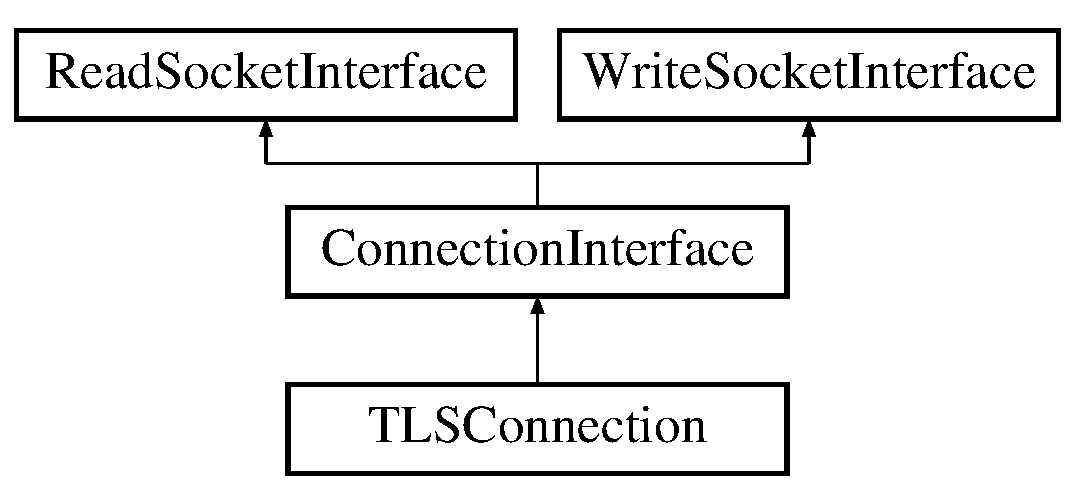
\includegraphics[height=3.000000cm]{class_t_l_s_connection}
\end{center}
\end{figure}
\subsection*{Public Member Functions}
\begin{DoxyCompactItemize}
\item 
\hyperlink{class_t_l_s_connection_ac9ad86b89b6a327277962f43a11b542e}{T\+L\+S\+Connection} (boost\+::asio\+::io\+\_\+service \&io\+\_\+service, const std\+::string \&scheme, const std\+::string \&server, const std\+::string \&port)
\item 
\mbox{\Hypertarget{class_t_l_s_connection_a3ee6b831efcf2674dc60ff29d9c5429d}\label{class_t_l_s_connection_a3ee6b831efcf2674dc60ff29d9c5429d}} 
{\bfseries T\+L\+S\+Connection} (boost\+::asio\+::io\+\_\+service \&io\+\_\+service)
\item 
\mbox{\Hypertarget{class_t_l_s_connection_a9fb660429140b86b36877afdbed4c1c0}\label{class_t_l_s_connection_a9fb660429140b86b36877afdbed4c1c0}} 
void {\bfseries async\+Connect} (Connect\+Callback\+Type cb)
\item 
\mbox{\Hypertarget{class_t_l_s_connection_a18acf6d17737221d72ad83ad9ec12bc9}\label{class_t_l_s_connection_a18acf6d17737221d72ad83ad9ec12bc9}} 
void {\bfseries async\+Accept} (boost\+::asio\+::ip\+::tcp\+::acceptor \&acceptor, std\+::function$<$ void(const boost\+::system\+::error\+\_\+code \&err)$>$ cb)
\item 
void \hyperlink{class_t_l_s_connection_abcca8739e56387ddceeefd15f8ea0967}{async\+Write} (\hyperlink{struct_m_buffer}{M\+Buffer} \&fb, Async\+Write\+Callback\+Type cb)
\item 
void \hyperlink{class_t_l_s_connection_a986b8ea40c6708966dc5a499e18b39ae}{async\+Write} (\hyperlink{class_f_buffer}{F\+Buffer} \&fb, Async\+Write\+Callback\+Type cb)
\item 
\mbox{\Hypertarget{class_t_l_s_connection_a5d7a765878b0087d3146cdc8fa97a5f5}\label{class_t_l_s_connection_a5d7a765878b0087d3146cdc8fa97a5f5}} 
void {\bfseries async\+Write\+Stream\+Buf} (boost\+::asio\+::streambuf \&sb, Async\+Write\+Callback)
\item 
void \hyperlink{class_t_l_s_connection_a37ef49d562cad83c9cdb130f7196f0b5}{async\+Read} (\hyperlink{struct_m_buffer}{M\+Buffer} \&mb, Async\+Read\+Callback\+Type cb)
\item 
\mbox{\Hypertarget{class_t_l_s_connection_aa8cac88c4c5108ab12c3f5399a3b630c}\label{class_t_l_s_connection_aa8cac88c4c5108ab12c3f5399a3b630c}} 
void {\bfseries shutdown} ()
\item 
\mbox{\Hypertarget{class_t_l_s_connection_acb98e7da74c8946ee1eb3dc29d60241a}\label{class_t_l_s_connection_acb98e7da74c8946ee1eb3dc29d60241a}} 
void {\bfseries close} ()
\item 
\mbox{\Hypertarget{class_t_l_s_connection_a871fe43f125797293bb7761268f94fe3}\label{class_t_l_s_connection_a871fe43f125797293bb7761268f94fe3}} 
long {\bfseries native\+Socket\+FD} ()
\item 
\mbox{\Hypertarget{class_t_l_s_connection_a20a96cc4b58864147634dba4236fdf94}\label{class_t_l_s_connection_a20a96cc4b58864147634dba4236fdf94}} 
std\+::string {\bfseries scheme} ()
\item 
\mbox{\Hypertarget{class_t_l_s_connection_a410ec7fcd5f42090531387893692f7e9}\label{class_t_l_s_connection_a410ec7fcd5f42090531387893692f7e9}} 
std\+::string {\bfseries server} ()
\item 
\mbox{\Hypertarget{class_t_l_s_connection_aa9f44a7552dfc1b04cb4056cefffb68d}\label{class_t_l_s_connection_aa9f44a7552dfc1b04cb4056cefffb68d}} 
std\+::string {\bfseries service} ()
\end{DoxyCompactItemize}


\subsection{Constructor \& Destructor Documentation}
\mbox{\Hypertarget{class_t_l_s_connection_ac9ad86b89b6a327277962f43a11b542e}\label{class_t_l_s_connection_ac9ad86b89b6a327277962f43a11b542e}} 
\index{T\+L\+S\+Connection@{T\+L\+S\+Connection}!T\+L\+S\+Connection@{T\+L\+S\+Connection}}
\index{T\+L\+S\+Connection@{T\+L\+S\+Connection}!T\+L\+S\+Connection@{T\+L\+S\+Connection}}
\subsubsection{\texorpdfstring{T\+L\+S\+Connection()}{TLSConnection()}}
{\footnotesize\ttfamily T\+L\+S\+Connection\+::\+T\+L\+S\+Connection (\begin{DoxyParamCaption}\item[{boost\+::asio\+::io\+\_\+service \&}]{io\+\_\+service,  }\item[{const std\+::string \&}]{scheme,  }\item[{const std\+::string \&}]{server,  }\item[{const std\+::string \&}]{port }\end{DoxyParamCaption})}

Constructor 
\begin{DoxyParams}{Parameters}
{\em \{io\+\_\+service\}} & io\+\_\+service -\/ to use for running \\
\hline
{\em \{string\}} & scheme -\/ \char`\"{}http\char`\"{} or \char`\"{}https\char`\"{} \\
\hline
{\em \{string\}} & server -\/ domain string \\
\hline
\end{DoxyParams}


\subsection{Member Function Documentation}
\mbox{\Hypertarget{class_t_l_s_connection_a37ef49d562cad83c9cdb130f7196f0b5}\label{class_t_l_s_connection_a37ef49d562cad83c9cdb130f7196f0b5}} 
\index{T\+L\+S\+Connection@{T\+L\+S\+Connection}!async\+Read@{async\+Read}}
\index{async\+Read@{async\+Read}!T\+L\+S\+Connection@{T\+L\+S\+Connection}}
\subsubsection{\texorpdfstring{async\+Read()}{asyncRead()}}
{\footnotesize\ttfamily void T\+L\+S\+Connection\+::async\+Read (\begin{DoxyParamCaption}\item[{\hyperlink{struct_m_buffer}{M\+Buffer} \&}]{buffer,  }\item[{Async\+Read\+Callback\+Type}]{cb }\end{DoxyParamCaption})\hspace{0.3cm}{\ttfamily [virtual]}}

read 

Implements \hyperlink{class_read_socket_interface}{Read\+Socket\+Interface}.

\mbox{\Hypertarget{class_t_l_s_connection_abcca8739e56387ddceeefd15f8ea0967}\label{class_t_l_s_connection_abcca8739e56387ddceeefd15f8ea0967}} 
\index{T\+L\+S\+Connection@{T\+L\+S\+Connection}!async\+Write@{async\+Write}}
\index{async\+Write@{async\+Write}!T\+L\+S\+Connection@{T\+L\+S\+Connection}}
\subsubsection{\texorpdfstring{async\+Write()}{asyncWrite()}\hspace{0.1cm}{\footnotesize\ttfamily [1/2]}}
{\footnotesize\ttfamily void T\+L\+S\+Connection\+::async\+Write (\begin{DoxyParamCaption}\item[{\hyperlink{struct_m_buffer}{M\+Buffer} \&}]{buffer,  }\item[{Async\+Write\+Callback\+Type}]{cb }\end{DoxyParamCaption})\hspace{0.3cm}{\ttfamily [virtual]}}

write 

Implements \hyperlink{class_connection_interface}{Connection\+Interface}.

\mbox{\Hypertarget{class_t_l_s_connection_a986b8ea40c6708966dc5a499e18b39ae}\label{class_t_l_s_connection_a986b8ea40c6708966dc5a499e18b39ae}} 
\index{T\+L\+S\+Connection@{T\+L\+S\+Connection}!async\+Write@{async\+Write}}
\index{async\+Write@{async\+Write}!T\+L\+S\+Connection@{T\+L\+S\+Connection}}
\subsubsection{\texorpdfstring{async\+Write()}{asyncWrite()}\hspace{0.1cm}{\footnotesize\ttfamily [2/2]}}
{\footnotesize\ttfamily void T\+L\+S\+Connection\+::async\+Write (\begin{DoxyParamCaption}\item[{\hyperlink{class_f_buffer}{F\+Buffer} \&}]{fb,  }\item[{Async\+Write\+Callback\+Type}]{cb }\end{DoxyParamCaption})}

use the boost function that O\+N\+LY returns when the write is D\+O\+NE 

The documentation for this class was generated from the following files\+:\begin{DoxyCompactItemize}
\item 
marvin/connection/tls\+\_\+connection.\+hpp\item 
marvin/connection/tls\+\_\+connection.\+cpp\end{DoxyCompactItemize}

\hypertarget{interface_traffic_for_host}{}\section{Traffic\+For\+Host Class Reference}
\label{interface_traffic_for_host}\index{Traffic\+For\+Host@{Traffic\+For\+Host}}
Inheritance diagram for Traffic\+For\+Host\+:\begin{figure}[H]
\begin{center}
\leavevmode
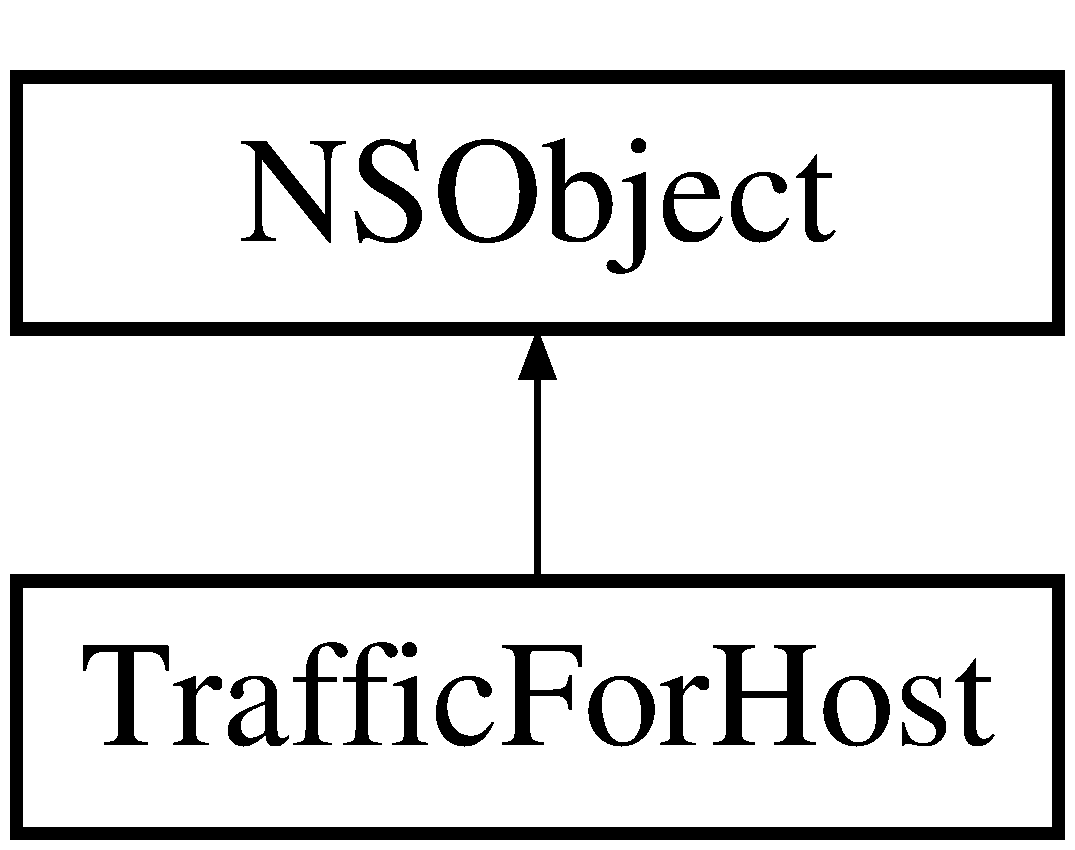
\includegraphics[height=2.000000cm]{interface_traffic_for_host}
\end{center}
\end{figure}
\subsection*{Instance Methods}
\begin{DoxyCompactItemize}
\item 
(id) -\/ {\bfseries init\+For\+Host\+:}
\item 
\mbox{\Hypertarget{interface_traffic_for_host_ae7df7efdaca12650330fc328a070da69}\label{interface_traffic_for_host_ae7df7efdaca12650330fc328a070da69}} 
(N\+S\+Array $\ast$) -\/ {\bfseries transactions}
\item 
\mbox{\Hypertarget{interface_traffic_for_host_aca1f0c56a9eec3fb20e5f4fe95383f10}\label{interface_traffic_for_host_aca1f0c56a9eec3fb20e5f4fe95383f10}} 
(void) -\/ {\bfseries add\+:}
\end{DoxyCompactItemize}
\subsection*{Properties}
\begin{DoxyCompactItemize}
\item 
\mbox{\Hypertarget{interface_traffic_for_host_a6d43931e2c34fa49aaf7597673a84860}\label{interface_traffic_for_host_a6d43931e2c34fa49aaf7597673a84860}} 
N\+S\+String $\ast$ {\bfseries host\+Name}
\end{DoxyCompactItemize}


\subsection{Method Documentation}
\mbox{\Hypertarget{interface_traffic_for_host_acf637083d9d1ae97550a6aa5ef73546d}\label{interface_traffic_for_host_acf637083d9d1ae97550a6aa5ef73546d}} 
\index{Traffic\+For\+Host@{Traffic\+For\+Host}!init\+For\+Host\+:@{init\+For\+Host\+:}}
\index{init\+For\+Host\+:@{init\+For\+Host\+:}!Traffic\+For\+Host@{Traffic\+For\+Host}}
\subsubsection{\texorpdfstring{init\+For\+Host\+:()}{initForHost:()}}
{\footnotesize\ttfamily -\/ (id) init\+For\+Host\+: \begin{DoxyParamCaption}\item[{(N\+S\+String$\ast$)}]{a\+Host }\end{DoxyParamCaption}}

{\bfseries Initial value\+:}
\begin{DoxyCode}
\{
    NSMutableArray* \_traffic
\end{DoxyCode}


The documentation for this class was generated from the following files\+:\begin{DoxyCompactItemize}
\item 
marvin/objc/traffic/Traffic\+For\+Host.\+h\item 
marvin/objc/traffic/Traffic\+For\+Host.\+m\end{DoxyCompactItemize}

\hypertarget{class_tunnel_handler}{}\section{Tunnel\+Handler Class Reference}
\label{class_tunnel_handler}\index{Tunnel\+Handler@{Tunnel\+Handler}}
\subsection*{Public Member Functions}
\begin{DoxyCompactItemize}
\item 
\mbox{\Hypertarget{class_tunnel_handler_a5168e90a221524fb993659159fa458e1}\label{class_tunnel_handler_a5168e90a221524fb993659159fa458e1}} 
{\bfseries Tunnel\+Handler} (Connection\+Interface\+S\+Ptr down\+Stream\+Connection, T\+C\+P\+Connection\+S\+Ptr upstream\+Connection)
\item 
void \hyperlink{class_tunnel_handler_aa734d9765344680b8c48bb0c2b870f72}{start} (std\+::function$<$ void(Marvin\+::\+Error\+Type \&err)$>$ cb)
\end{DoxyCompactItemize}


\subsection{Member Function Documentation}
\mbox{\Hypertarget{class_tunnel_handler_aa734d9765344680b8c48bb0c2b870f72}\label{class_tunnel_handler_aa734d9765344680b8c48bb0c2b870f72}} 
\index{Tunnel\+Handler@{Tunnel\+Handler}!start@{start}}
\index{start@{start}!Tunnel\+Handler@{Tunnel\+Handler}}
\subsubsection{\texorpdfstring{start()}{start()}}
{\footnotesize\ttfamily void Tunnel\+Handler\+::start (\begin{DoxyParamCaption}\item[{std\+::function$<$ void(Marvin\+::\+Error\+Type \&err)$>$}]{cb }\end{DoxyParamCaption})}

start both halves, downstream first as there is not likely to be traffic that way until the upstream starts we are done when they are both done the error to record is the one that strikes first. we done need to force close anything as the servers ro client should eventually close their end and we will ehar about it 

The documentation for this class was generated from the following files\+:\begin{DoxyCompactItemize}
\item 
marvin/connection/tunnel\+\_\+handler.\+hpp\item 
marvin/connection/tunnel\+\_\+handler.\+cpp\end{DoxyCompactItemize}

\hypertarget{class_uri_query}{}\section{Uri\+Query Class Reference}
\label{class_uri_query}\index{Uri\+Query@{Uri\+Query}}
\subsection*{Public Member Functions}
\begin{DoxyCompactItemize}
\item 
\mbox{\Hypertarget{class_uri_query_a312cab0b9f2e254524ebe10e1c8e4315}\label{class_uri_query_a312cab0b9f2e254524ebe10e1c8e4315}} 
{\bfseries Uri\+Query} (std\+::string q\+\_\+str)
\item 
\mbox{\Hypertarget{class_uri_query_a8256a0db97478d0573c01ba42f0a47f4}\label{class_uri_query_a8256a0db97478d0573c01ba42f0a47f4}} 
void {\bfseries parse} (std\+::string s)
\item 
\mbox{\Hypertarget{class_uri_query_ac865497506e613143548d7d4c1a6f49e}\label{class_uri_query_ac865497506e613143548d7d4c1a6f49e}} 
std\+::string \& {\bfseries str} ()
\item 
\mbox{\Hypertarget{class_uri_query_a60c9ffd3f4336b57ca7aae3242c59157}\label{class_uri_query_a60c9ffd3f4336b57ca7aae3242c59157}} 
std\+::map$<$ std\+::string, std\+::string $>$ \& {\bfseries key\+Values} ()
\end{DoxyCompactItemize}


The documentation for this class was generated from the following files\+:\begin{DoxyCompactItemize}
\item 
marvin/message/uri\+\_\+query.\+hpp\item 
marvin/message/uri\+\_\+query.\+cpp\end{DoxyCompactItemize}

\hypertarget{class_waiting_requests_type}{}\section{Waiting\+Requests\+Type Class Reference}
\label{class_waiting_requests_type}\index{Waiting\+Requests\+Type@{Waiting\+Requests\+Type}}
\subsection*{Public Member Functions}
\begin{DoxyCompactItemize}
\item 
\mbox{\Hypertarget{class_waiting_requests_type_a790ddd29bf0e552abf72ce25b45bc922}\label{class_waiting_requests_type_a790ddd29bf0e552abf72ce25b45bc922}} 
std\+::size\+\_\+t {\bfseries size} ()
\item 
\mbox{\Hypertarget{class_waiting_requests_type_a03b3e374d7bfdf7dbd5090e304098120}\label{class_waiting_requests_type_a03b3e374d7bfdf7dbd5090e304098120}} 
\hyperlink{class_connection_request}{Connection\+Request} $\ast$ {\bfseries find} (std\+::string scheme, std\+::string server, std\+::string service)
\item 
\mbox{\Hypertarget{class_waiting_requests_type_a629d54b7847918da2e7343d24cf5e11d}\label{class_waiting_requests_type_a629d54b7847918da2e7343d24cf5e11d}} 
\hyperlink{class_connection_request}{Connection\+Request} $\ast$ {\bfseries remove\+Oldest} ()
\item 
\mbox{\Hypertarget{class_waiting_requests_type_afb37d267af782b4e03525bd785a6be98}\label{class_waiting_requests_type_afb37d267af782b4e03525bd785a6be98}} 
void {\bfseries add} (\hyperlink{class_connection_request}{Connection\+Request} $\ast$conn\+Req)
\item 
\mbox{\Hypertarget{class_waiting_requests_type_a790ddd29bf0e552abf72ce25b45bc922}\label{class_waiting_requests_type_a790ddd29bf0e552abf72ce25b45bc922}} 
std\+::size\+\_\+t {\bfseries size} ()
\item 
\mbox{\Hypertarget{class_waiting_requests_type_a1891f7c90dc587d550491db111c53c90}\label{class_waiting_requests_type_a1891f7c90dc587d550491db111c53c90}} 
\hyperlink{class_connection_request}{Connection\+Request} $\ast$ {\bfseries find} (std\+::string scheme, std\+::string server, std\+::string service)
\item 
\mbox{\Hypertarget{class_waiting_requests_type_a46aee62e2e9ca030c5c13243cc2d88da}\label{class_waiting_requests_type_a46aee62e2e9ca030c5c13243cc2d88da}} 
\hyperlink{class_connection_request}{Connection\+Request} $\ast$ {\bfseries remove\+Oldest} ()
\item 
\mbox{\Hypertarget{class_waiting_requests_type_afb37d267af782b4e03525bd785a6be98}\label{class_waiting_requests_type_afb37d267af782b4e03525bd785a6be98}} 
void {\bfseries add} (\hyperlink{class_connection_request}{Connection\+Request} $\ast$conn\+Req)
\end{DoxyCompactItemize}


The documentation for this class was generated from the following files\+:\begin{DoxyCompactItemize}
\item 
marvin/connection/connection\+\_\+pool.\+hpp\item 
marvin/server/connection\+\_\+handler\+\_\+pool.\+hpp\item 
marvin/connection/connection\+\_\+pool.\+cpp\item 
marvin/server/connection\+\_\+handler\+\_\+pool .\+cpp\end{DoxyCompactItemize}

\hypertarget{class_write_socket_interface}{}\section{Write\+Socket\+Interface Class Reference}
\label{class_write_socket_interface}\index{Write\+Socket\+Interface@{Write\+Socket\+Interface}}
Inheritance diagram for Write\+Socket\+Interface\+:\begin{figure}[H]
\begin{center}
\leavevmode
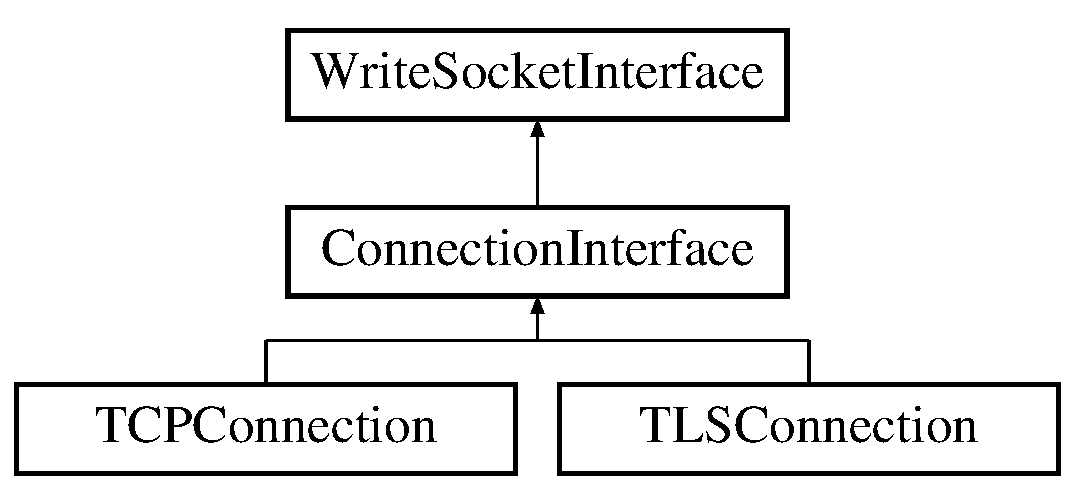
\includegraphics[height=3.000000cm]{class_write_socket_interface}
\end{center}
\end{figure}
\subsection*{Public Member Functions}
\begin{DoxyCompactItemize}
\item 
\mbox{\Hypertarget{class_write_socket_interface_a3eccd4e4d2ba0f5ca8528114f53dc178}\label{class_write_socket_interface_a3eccd4e4d2ba0f5ca8528114f53dc178}} 
virtual long {\bfseries native\+Socket\+FD} ()=0
\item 
\mbox{\Hypertarget{class_write_socket_interface_abe92a0daa62bf30872c3655f4c1ce17b}\label{class_write_socket_interface_abe92a0daa62bf30872c3655f4c1ce17b}} 
virtual void {\bfseries async\+Write} (\hyperlink{struct_m_buffer}{M\+Buffer} \&fb, Async\+Write\+Callback)=0
\item 
\mbox{\Hypertarget{class_write_socket_interface_a00e0406455f67da23061ec429e56528d}\label{class_write_socket_interface_a00e0406455f67da23061ec429e56528d}} 
virtual void {\bfseries async\+Write} (Buffer\+Chain\+S\+Ptr chain\+\_\+sptr, Async\+Write\+Callback)=0
\item 
\mbox{\Hypertarget{class_write_socket_interface_a7e8ef6da94a56889a7ad6d7490fc1ebb}\label{class_write_socket_interface_a7e8ef6da94a56889a7ad6d7490fc1ebb}} 
virtual void {\bfseries async\+Write} (boost\+::asio\+::const\+\_\+buffer buf, Async\+Write\+Callback cb)=0
\item 
\mbox{\Hypertarget{class_write_socket_interface_af38fe8608053b52b086f6a063cef8b4a}\label{class_write_socket_interface_af38fe8608053b52b086f6a063cef8b4a}} 
virtual void {\bfseries async\+Write} (boost\+::asio\+::streambuf \&sb, Async\+Write\+Callback)=0
\end{DoxyCompactItemize}


The documentation for this class was generated from the following file\+:\begin{DoxyCompactItemize}
\item 
marvin/include/read\+\_\+socket\+\_\+interface.\+hpp\end{DoxyCompactItemize}

%--- End generated contents ---

% Index
\backmatter
\newpage
\phantomsection
\clearemptydoublepage
\addcontentsline{toc}{chapter}{Index}
\printindex

\end{document}
